\documentclass[article]{jss}
%% -- LaTeX packages and custom commands ---------------------------------------

\usepackage[usenames,dvipsnames]{xcolor}

%% recommended packages
\usepackage{thumbpdf,lmodern}
\usepackage{orcidlink}
\usepackage{amsmath,amssymb,bbold, xfrac}

\usepackage{multirow}
\usepackage{caption}
\usepackage{subcaption} % for subfigure
\usepackage{float}

%% TikZ packages
\usepackage{tikz}
\usetikzlibrary{shapes.geometric, arrows, backgrounds, scopes}
\usepackage{pgfplots}
\pgfplotsset{width=6.75cm, compat=newest}
\usepackage[utf8]{inputenc}
\DeclareUnicodeCharacter{2212}{−}
\usepgfplotslibrary{groupplots,dateplot}
\usetikzlibrary{patterns,shapes.arrows}

%% for algorithms
\usepackage{algorithm}
\usepackage{algpseudocode} % algorithmicx package

%% another package (only for this demo article)
\usepackage{framed}
\usepackage{marginnote}

%% new custom commands
\newcommand{\class}[1]{`\code{#1}'}
\newcommand{\fct}[1]{\code{#1()}}

%% Vasilis' custom commands
\newcommand{\bigO}{\mathcal{O}}
\newcommand{\X}{\mathbf{x}}
\newcommand{\Z}{\mathbf{z}}
\newcommand{\V}{\mathbf{V}}
\newcommand{\Y}{\mathbf{Y}}
\newcommand{\hess}{\mathbf{H}}
\newcommand{\Thetab}{\mathbf{\Theta}}

\newcommand{\vb}{\mathbf{v}}
\newcommand{\ub}{\mathbf{u}}
\newcommand{\yb}{\mathbf{y}}
\newcommand{\xb}{\mathbf{x}}

\newcommand{\jac}{\mathbf{J}}
\newcommand{\hessian}{\mathbf{H}}
\newcommand{\thetab}{\boldsymbol{\theta}}
\newcommand{\thetabij}{\thetab_{ij}}
\newcommand{\thetabi}{\thetab_i}

\newcommand{\simulator}{g}
\newcommand{\region}{B_{d,\epsilon}}
\newcommand{\indicator}[1]{\mathbb{1}_{#1}}
\newcommand{\regioni}{B_{d,\epsilon}^i}
\newcommand{\data}{\mathbf{y_0}}
\newcommand{\accregioni}{C^i_{\epsilon}}
\newcommand{\accregionihat}{\hat{C}^i_{\epsilon}}

\newcommand{\danger}{\fontencoding{U}\fontfamily{futs}\selectfont\char 66\relax}
\newcommand{\TODO}[1]{\textcolor{red}{TODO #1}\marginpar{\textcolor{red}{\Large \danger}}}


\newcommand{\R}{\mathbb{R}}

\newcommand{\Ex}{\mathbb{E}}

\DeclareMathOperator*{\argmax}{argmax}
\DeclareMathOperator*{\argmin}{argmin}

%% -- Article metainformation (author, title, ...) -----------------------------

\author{Vasilis Gkolemis~\orcidlink{0000-0002-2636-0245}\\ATHENA RC \And
  Michael Gutmann~\orcidlink{0000-0002-5329-9910}\\University of Edinburgh \And
  Henri Pesonen~\orcidlink{0000-0003-4500-2926}\\University of Oslo}

\Plainauthor{Vasilis Gkolemis, Michael Gutmann, Henri Pesonen}

\title{An Extendable \proglang{Python} Implementation of Robust Optimisation Monte Carlo}
\Plaintitle{An Extendable Python Implementation of ROMC}
\Shorttitle{An Extendable ROMC implementation}

%% - \Abstract{} almost as usual
\Abstract{Performing inference in statistical models with an
  intractable likelihood is challenging, therefore, most
  likelihood-free inference (LFI) methods encounter accuracy and
  efficiency limitations. In this paper, we present the implementation
  of the LFI method Robust Optimisation Monte Carlo (ROMC) in the
  \proglang{Python} package \pkg{ELFI}. ROMC is a novel and efficient
  (highly-parallelisable) LFI framework that provides accurate
  weighted samples from the posterior. Our implementation can be used
  in two ways. First, a scientist may use it as an out-of-the-box LFI
  algorithm; we provide an easy-to-use API harmonised with the
  principles of \pkg{ELFI}, enabling effortless comparisons with the
  rest of the methods included in the package. Additionally, we have
  carefully split ROMC into isolated components for supporting
  extensibility. A researcher may experiment with novel method(s) for
  solving part(s) of ROMC without reimplementing everything from
  scratch. In both scenarios, the ROMC parts can run in a
  fully-parallelised manner, exploiting all CPU cores. We also provide
  helpful functionalities for (i) inspecting the inference process and
  (ii) evaluating the obtained samples. Finally, we test the
  robustness of our implementation on some typical LFI examples.}

%% - \Keywords{}
\Keywords{Bayesian inference, implicit models, likelihood-free, \proglang{Python}, \pkg{ELFI}}
\Plainkeywords{Bayesian inference, implicit models, likelihood-free, Python, ELFI}

%% - \Address{} of at least one author
\Address{
  Vasilis Gkolemis\\
  Information Management Systems Institute (IMSI)\\
  ATHENA Research and Innovation Center\\
  Athens, Greece\\
  E-mail: \email{vgkolemis@athenarc.gr}\\
  URL: \url{https://givasile.github.io}
}

\begin{document}

%% -- Introduction -------------------------------------------------------------
\section{Introduction} \label{sec:intro}

Simulator-based models are particularly captivating due to the
provided modeling freedom. In essence, any data generating mechanism
that can be written as a finite set of algorithmic steps can be
programmed as a simulator-based model. In these cases, it is feasible
to generate samples using the simulator but it is infeasible to
evaluate the likelihood function. The intractability of the likelihood
makes the likelihood-free inference (LFI), i.e., the approximation of
the posterior distribution without using the likelihood function,
particularly challenging.

Optimization Monte Carlo (OMC) proposed by~\citet{Meeds2015} is a
novel LFI approach for approximating the posterior distribution. The
central idea is turning the stochastic data-generating mechanism into
a set of deterministic optimization processes. Afterwards,
\citet{Forneron2016} provided a similar method under the name `reverse
sampler'. In their work,~\citet{Ikonomov2019}, located some critical
limitations of OMC, so they proposed Robust OMC (ROMC), an alternative
version of OMC with the appropriate modifications.

In this paper, we present the implementation of ROMC at the
\proglang{Python} package \pkg{ELFI} (Engine for likelihood-free
inference)~\citet{1708.00707}. As we illustrate at
Section~\ref{sec:implementation}, we have carefully designed the
implementation to ensure extensibility. ROMC is a general framework
for obtaining weighted samples from the posterior, i.e., it defines a
sequence of algorithmic steps without enforcing a specific algorithm
for solving each step. Therefore, a researcher may use ROMC as the
backbone algorithm and develop novel methods to solve each separate
step.\footnote{For being a ready-to-use
algorithm,~\citet{Ikonomov2019} proposed a default method for each
step, but this choice is by no means restrictive.} We have designed
our software for facilitating such experimentation.

To the best of our knowledge, this is the first implementation of the
ROMC inference method to a generic LFI framework. We organize the
evaluation in three steps. First, for securing that our implementation
is accurate, we test it against an artificial example with a tractable
likelihood. The artificial example also serves as a step-by-step guide
for showcasing how to use the various functionalities of our
implementation. Second, we use the second-order moving average (MA2)
example from the \pkg{ELFI} package, using as ground truth the samples
obtained with Rejection ABC~\citet{lintusaari2017}, with a very large
number of trials. Finally, we present the execution times of ROMC,
measuring the speed-up obtained by using the parallel version of the
implementation.

% \clearpage
\section{Background}

We first give a short introduction to simulator-based models, we then
focus on OMC and its robust improvement, ROMC, and we, finally,
introduce \pkg{ELFI}, the underlying package that is used for the
implementation of ROMC.

\subsection{Simulator-based models and likelihood-free inference}

An implicit or simulator-based model is a parameterized stochastic
data generating mechanism. The key characteristic of simulator-based
models is that we can sample data points, but we cannot evaluate the
likelihood. Formally, a simulator-based model is a parameterized
family of probability density functions
\(\{ p(\yb|\thetab)\}_{\thetab}\) whose closed-form is either unknown
or computationally intractable. In these scenarios, we can only a
access the simulator \( m_r(\thetab) \), i.e., the black-box mechanism
(computer code) that generates samples \(\yb\) in a stochastic manner
from a set of parameters \(\thetab\). We denote the process of
obtaining samples from the simulator with
\( m_r(\thetab) \rightarrow \yb \). As shown by~\citet{Meeds2015}, it
is feasible to isolate the randomness of the simulator by introducing
a set of nuisance random variables denoted by \(\ub \sim
p(\ub)\). Therefore, for a specific tuple \((\thetab, \ub)\) the
simulator becomes a deterministic mapping \(g\), such that
\(\yb=\simulator(\thetab,\ub)\). In terms of computer code, the
stochasticity of a random process is governed by the global
seed. Although each software may handle the randomness in slightly
different ways\footnote{For example, at
  \pkg{Numpy}~\citet{harris2020array}, the pseudo-random number
  generation is based on a global state, whereas, in
  \pkg{JAX}~\citet{jax2018github} random functions consume a key that
  is passed as parameter. }, in all cases, freezing the initial seed
to a specific integer converts the simulation to a deterministic piece
of code.

Simulator-based models provide modeling freedom, including hidden
(unobserved) random variables or rule-based decisions. In fact, any
physical process that can be conceptualized as a computer program of
finite steps can be modeled as a simulator-based model. Hence,
implicit models are often used to model physical phenomena in the
natural sciences such as, e.g., genetics, epidemiology or
neuroscience. Further background on simulator-based models and example
applications can be found in the articles by~\citet{gutmann2016,
  lintusaari2017, sisson2018, cranmer2020}.

The modeling freedom of simulator-based models, however, comes at the
price of difficulties in inferring the parameters of
interest. Denoting the observed data as \(\data\), the main difficulty
lies at the intractability of the likelihood function
\(L(\thetab) = p(\data|\thetab)\). To better see the sources of the
intractability, and to address them, we go back to the basic
characterization of the likelihood as the (rescaled) probability of
generating data \(\yb\) that is similar to the observed data
\(\data\), using parameters \(\thetab\). Formally, the likelihood
\(L(\thetab)\) equals

\begin{equation}
  \label{eq:likelihood}
  L(\thetab) = \lim_{\epsilon \to 0} c_\epsilon \int_{\yb \in B_{d,\epsilon}(\data)} p(\yb|\thetab)d\yb =
  \lim_{\epsilon \to 0} c_\epsilon \Pr(\simulator(\thetab, \ub) \in \region(\data)  \mid \theta)
\end{equation}
where \(c_\epsilon\) is a proportionality factor that depends on
\(\epsilon\) and \(\region(\data)\) is an \(\epsilon\) region around
\(\data\) that is defined through a distance function \(d\), i.e., \
\(\region(\data) := \{\yb: d(\yb, \data) \leq \epsilon \}\).

Equation~\ref{eq:likelihood} highlights the main source of
intractability; computing
\(\Pr(\simulator(\thetab,\ub) \in \region(\data)) | \thetab\) as the
fraction of samples that lie inside the \(\epsilon\) region around
\(\data\) is computationally infeasible in the limit of
\(\epsilon \to 0\). Hence, the constrainted is relaxed to
\(\epsilon > 0\), which leads to the approximate likelihood:

\begin{equation}
  \label{eq:approx_likelihood}
  L_{d, \epsilon}(\thetab) = \Pr(\yb \in \region(\data) \mid \theta), \quad \text{where  } \epsilon > 0.
\end{equation}

and, in turn, to the approximate posterior:

\begin{equation} \label{eq:approx_posterior}
  p_{d,\epsilon}(\thetab|\data)
  \propto L_{d, \epsilon}(\thetab) p(\thetab)
  \propto L_{d, \epsilon}(\thetab) p(\thetab)
\end{equation}

The approximation in
Equations~\ref{eq:approx_likelihood},~\ref{eq:approx_posterior} is by
no means the only strategy to deal with the intractability of the
likelihood function in Equation~\ref{eq:likelihood}. Other strategies include
modeling the (stochastic) relationship between \(\thetab\) and
\(\yb\), and its reverse, or framing likelihood-free inference as a
ratio estimation problem, see for example \citet{blum2010, Wood2006,
  Papamakarios2016, Papamakarios2019, Chen2019, Thomas2020,
  Hermans2020}. However, both OMC and robust OMC, which we introduce
next, are based on the approximation in Equation~\ref{eq:approx_likelihood}.

\subsection{Optimization Monte Carlo (OMC)}

Our description of OMC~\citet{Meeds2015}
follows~\citet{Ikonomov2019}. We define the indicator function (boxcar
kernel) that equals one only if \(\xb\) lies in \(\region(\yb)\):
%
\begin{equation}
  \label{eq:indicator}
  \indicator{\region(\yb)}(\xb)=
  \left\{
    \begin{array}{ll}
      1 & \mbox{if } \xb \in \region(\yb) \\
      0 & \mbox{otherwise}
    \end{array} \right. \end{equation}
%

We, then, rewrite the approximate likelihood function
\(L_{d, \epsilon}(\thetab)\) of Equation~\ref{eq:approx_likelihood} as:

\begin{gather}
  \label{eq:approx_likelihood_omc}
  L_{d, \epsilon}(\thetab) = \Pr(\yb \in \region(\data) | \thetab) =
  \int_{\ub} \indicator{\region(\data)}(g(\thetab, \ub)) d \ub
\end{gather}

which can be approximated using samples from the simulator:

\begin{equation}
  \label{eq:samples_approx_likelihood_omc}
  L_{d, \epsilon}(\thetab) \approx \frac{1}{N} \sum_{i=1}^N \indicator{\region (\data)} (\simulator(\thetab, \ub_i))
 \quad \text{ where } \ub_i \sim p(\ub).
\end{equation}

In Equation~\ref{eq:samples_approx_likelihood_omc}, for each
\(\ub_i\), there is a region \(\accregioni\) in the parameter space
\(\thetab\) where the indicator function returns one, i.e.,
\(\accregioni = \{ \thetab: \simulator(\thetab, \ub_i) \in
\region(\data) \}\). Therefore, we can approximate the likelihood as:

\begin{equation}
  \label{eq:alt_view_theta}
  L_{d, \epsilon}(\thetab) \approx \frac{1}{N} \sum_{i=1}^N \indicator{\accregioni}(\thetab)
\end{equation}

and the corresponding approximate posterior:

\begin{equation}
  \label{eq:approx_posterior_omc}
  p_{d,\epsilon}(\thetab|\data) \propto
  p(\thetab) \sum_i^N  \indicator{\accregioni}(\thetab).
\end{equation}

As argued by \citet{Ikonomov2019}, these derivations provide a unique
perspective for likelihood-free inference by shifting the focus onto
the geometry of the acceptance regions \(\accregioni\). Indeed, the
task of approximating the likelihood and the posterior becomes a task
of characterising the sets \(\accregioni\). OMC by \citet{Meeds2015}
assumes that the distance \(d\) is the Euclidean distance
\(||\cdot||_2\) between summary statistics \(\Phi\) of the observed
and generated data, and that the \(\accregioni\) can be well
approximated by infinitesimally small ellipses. These assumptions lead
to an approximation of the posterior in terms of weighted samples
\(\thetab_i^*\) that achieve the smallest distance between observed
and simulated data for each realisation \(\ub_i \sim p(\ub)\), i.e.,\
\begin{equation} \label{eq:omc_opt_prob}
\thetab_i^* = \argmin_{\thetab} ||\Phi(\data)-\Phi(\simulator(\thetab, \ub_i))||_2  , \quad \ub_i \sim p(\ub).
\end{equation}
The weighting for each \(\thetab_i^*\) is proportional to the prior
density at \(\thetab_i^*\) and inversely proportional to the determinant
of the Jacobian matrix of the summary statistics at \(\thetab_i^*\). For
further details on OMC we refer the reader to \citep{Meeds2015,
  Ikonomov2019}.



\subsection{Robust optimization Monte Carlo (ROMC)}

\citet{Ikonomov2019} showed that considering infinitesimally small
ellipses can lead to highly overconfident posteriors. We refer the
reader to their paper for the technical details and conditions for
this issue to occur. Intuitively, it happens because the weights in
OMC are only computed from information at \(\thetab_i^*\), and using
only local information can be misleading. For example if the curvature
of \(||\Phi(\data)-\Phi(\simulator(\thetab, \ub_i))||_2\) at
\(\thetab_i^*\) is nearly flat, the curvature alone may wrongly
indicate that \(\accregioni\) is much larger than it actually is. In
our software package we implement the robust generalisation of OMC by
\citet{Ikonomov2019} that resolves this issue.

ROMC, firstly, approximates the acceptance regions \(\accregioni\),
and defines proposal distributions \(q_i(\thetab)\) on them. The
proposal distributions are used for generating posterior samples
\(\thetab_{ij} \sim q_i\). The samples are assigned (importance)
weights \(w_{ij}\) that compensate for using the proposal
distributions \(q_i(\thetab)\) and not the prior \(p(\thetab)\),
\begin{equation}
  w_{ij} = \frac{\indicator{\accregioni}(\thetab_{ij}) p(\thetab_{ij})}{q(\thetab_{ij})}.
  \label{eq:sampling}
\end{equation}
Given the weighted samples, any expectation
\(\E_{p(\thetab|\data)}[h(\thetab)]\) of some function \(h(\thetab)\), can be approximated as
\begin{equation} \label{eq:expectation}
  \E_{p(\thetab|\data)}[h(\thetab)] \approx \frac{\sum_{ij} w_{ij} h(\thetab_{ij})}{\sum_{ij} w_{ij}}
\end{equation}
\citet{Ikonomov2019} considered uniform distributions as proposal
distributions so that the main task is to approximate the acceptance
regions \(\accregioni\) and to represent them so that uniform sampling
is easy. The approximation of the acceptance regions contains two
compulsory and one optional step: (1) solving the optimisation
problems as in OMC, (2) constructing bounding boxes around
\(\accregioni\) and optionally, (3) refining the approximation via a
surrogate model of the distance.

\subsubsection*{Solving the deterministic optimisation problems}
For each set of nuisance variables \(\ub_i, i = \{1,2,\ldots,n_1 \}\),
we search for a point \(\thetab^*_i\) such that
\(d(\simulator(\thetab^*_i,\ub_i), \data) \le \epsilon\). In general,
\(d\) can be any valid distance, but for the rest of the paper we
consider \(d\) as the squared Euclidean distance. For notational
convenience, we denote \(d(\simulator(\thetab,\ub_i), \data)\) as
\(d_i(\thetab)\).  Obtaining \(\theta_i^*\) involves solving the
following optimisation problem:
\begin{subequations}
\begin{alignat}{2}
  &\!\min_{\thetab}        && d_i(\thetab) \label{eq:optProb}\\
  &\text{subject to} & \quad& d_i(\thetab) \leq \epsilon
\end{alignat}
\end{subequations}
%
The optimisation problem can be treated as unconstrained, accepting
the optimal point
\(\thetab_i^* = \text{argmin}_{\thetab} d_i(\thetab)\) only if
\(d_i(\thetab_i^*) \le \epsilon\). If \(d_i(\thetab)\) is
differentiable any gradient-based optimizer can be used
for~\ref{eq:optProb}. The gradients \(\nabla_{\thetab} d_i(\thetab)\)
can be either provided in closed form or approximated by finite
differences. In case \(d_i\) is not differentiable, Bayesian
Optimisation~\citep{Shahriari2016} provides an alternative
approach. In this scenario, apart from obtaining an optimal
\(\thetab_i^* \), a surrogate model \(\hat{d}_i(\thetab)\) of the
distance function \(d_i(\thetab)\) is also automatically obtained;
\(\hat{d}_i\) can then substitute the actual distance function in
downstream steps of the algorithms, with possible computational gains
especially if evaluating the actual distance \(d_i(\thetab)\) is
expensive.

\subsubsection*{Estimating the acceptance regions}
The acceptance region \(\accregioni\) is approximated by a bounding
box \(\accregionihat\). Ideally, we want the bounding box to be as
tight as possible to \(\accregioni\) to ensure high acceptance rate in
the importance sampling, but big enough for not discarding valid
parts. The bounding boxes are built in two steps. First, we define
their axes \(\mathbf{v}_m\), \(m = \{1, \ldots, D\}\) based on the
(estimated) curvature of the distance at \(\thetab_i^*\). Second, we
determine the size of the box via a one-dimensional line-search method
along each axis, see Algorithm~\ref{alg:region_construction} for the
details. After the bounding boxes construction, a uniform distribution
\(q_i\) is defined on each bounding box, and is used as the proposal
region for importance sampling.

\subsubsection*{Refining the estimate via a local surrogate model (optional)}
When computing the weight \(w_{ij}\) in \eqref{eq:sampling}, we need
to check whether the samples \(\thetab_{ij} \sim q_i\) lie inside the
acceptance region \(\accregioni\). This can be considered to be a
safety-mechanism that corrects for any inaccuracies in the
construction of \(\accregionihat\) above. However, this check involves
evaluting the distance function \(d_i(\thetab_{ij})\), which can be
expensive if the model is complex. \citet{Ikonomov2019} thus proposed
to fit a surrogate model \(\tilde{d}_i(\thetab)\) of the distance
function \(d_i(\thetab)\), on data points that lie inside
\(\accregionihat\). They used a simple quadratic model whilst other
regression models are, in principle, possible too. The advantage of
using a quadratic model is that it has ellipsoidal isocontours, which
thus naturally allowed \citet{Ikonomov2019} to replace the bounding
box approximation of \(\accregioni\) with a tigher-fitting ellipsoidal
approximation.\footnote{The difference to the infinitesimal
  ellipsoidal model in OMC is the estimation procedure: OMC uses
  information at \(\thetab_i^*\) whilst, here, information in
  \(\accregionihat\) is used, which results in a more stable fit.}

The training data for the quadratic model is obtained by sampling
\(\thetab_{ij} \sim q_i\) and accessing the distances
\(d_i(\thetab_{ij})\). The generation of the training data adds an
extra computational cost, but leads to a significant speed-up when
evaluating the weights \(w_{ij}\). Moreover, the extra cost is largely
eliminated if Bayesian Optimisation with a Gaussian process (GP)
surrogate model \(\hat{d}_i(\thetab)\) was used to obtain
\(\thetab_i^*\) in the first step. In this case, we can use
\(\hat{d}_i(\thetab)\) instead of \(d_i(\thetab)\) to generate the
training data. This essentially replaces the global GP model with a
simpler local quadratic model which is typically more robust.


\subsection[Engine for likelihood-free inference (ELFI)]{\pkg{Engine for likelihood-free inference (ELFI)}}
\label{subsec:ELFI}
\pkg{Engine for Likelihood-Free Inference (ELFI)}\footnote{Extended
  documentation can be found
  \href{https://elfi.readthedocs.io/en/latest/}{https://elfi.readthedocs.io}}~\cite{1708.00707}
is a \proglang{Python} package for LFI. We
selected to implemented ROMC in \pkg{ELFI} since it provides
convenient modules for all the fundamental components of a
probabilistic model (e.g.\ prior, simulator, summaries
etc.). Furthermore, \pkg{ELFI} already supports some recently proposed
likelihood-free inference methods, making it straightforward to
perform comparisons between methods.

% \subsubsection{Modelling at ELFI}
% \label{sec:modelling}

\pkg{ELFI} handles the probabilistic model as a Directed Acyclic Graph
(DAG). This functionality is based on the package
\pkg{NetworkX}~\cite{hagberg2008exploring}, which supports
general-purpose graphs. In most cases, the structure of a
likelihood-free model follows the pattern of Figure~\ref{fig:elfi};
some edges connect the prior distributions to the simulator, the
simulator is connected to the summary statistics that, in turn, lead
to the output node. Samples can be obtained from all nodes through
sequential (ancestral) sampling. \pkg{ELFI} automatically considers as
parameters of interest, i.e. those we try to infer a posterior
distribution, as the ones defined through the \code{elfi.Prior}
class. Finally, the observations are passed to the appropriate node
through the argument \code{observed}.

\begin{figure}[ht]
    \begin{center}
      \includegraphics[width=0.8\textwidth]{./latex_files/images/chapter2/elfi.png}
    \end{center}
    \caption[Baseline example for creating an \pkg{ELFI} model]{Baseline example for creating an \pkg{ELFI} model. Image taken from \cite{1708.00707}}
    \label{fig:elfi}
\end{figure}

% \subsubsection{Inference at ELFI}
% \label{sec:inference-methods}

All inference methods in \pkg{ELFI} share the following rules;

\begin{itemize}
\item they follow the signature \code{elfi.<Class name>(<output node>,
    *arg)}; the initial argument is the output node model and the rest
  of the arguments are hyper-parameters of the method.
\item they provide a central sampling functionality, which in most
  cases is named \\ \code{<method_name>.sample()}.
\end{itemize}


%% -- Design Principles -----------------------------------------------------
\section{Implementation}
\label{sec:implementation}
This section is split in two parts. We first express ROMC as an
algorithm and then we present the general implementation principles we
follow.

\subsection{Algorithmic view of ROMC}
For designing an extendable implementation of ROMC, we firstly define
ROMC as a sequence of algorithmic steps. The algorithmic view of ROMC
serves as the driver for the implementation at \pkg{ELFI}. At a high
level, ROMC can be split into the training and the inference part. In
general terms, the training part covers all steps for estimating the
proposal regions and the inference part calculates the weighted
samples. Algorithm~\ref{alg:romc_algorithm} defines ROMC formally;
Steps 2-10 (before the horizontal line) and steps 12-17 form the training 
part and the inference part, respectively. \textbf{HP comment Algorithm 1: I got a bit 
lost with $M_r(\thetab)$ (Line 1) and $M_d(\thetab, \vb=\vb_i)$ (Line 4). 
What is their relationship? Also, are Lines 13, 16 and 17 still under construction?
Maybe refer to Eq. (X)s in the Algorithm, if wanting to keep the Algorithm compact.}

\begin{algorithm}[!ht]
	\caption{ROMC}\label{alg:romc_algorithm}
	\begin{algorithmic}[1]
    \Procedure{ROMC}{$M_r(\thetab), n_1, n_2, \epsilon$}
    \For{$i \gets 1 \textrm{ to } n_1$}
      \State $\vb_i \sim p(\vb)$ \Comment{Draw nuisance variables}
      \State $d_i(\thetab) = M_d(\thetab, \vb=\vb_i)$ \Comment{Define distance function}
      \State $\thetab_i^* = \text{argmin}_{\thetab} d_i$, $d_i^*=d_i(\thetab_i^*)$ \Comment{Solve optimisation problem}
      \If{$d^*_i > \epsilon$}
        \State Go to 2 \Comment{Filter solution}
      \EndIf
      \State Define $q_i$ over $\mathcal{\hat{S}}$ \Comment{Estimate proposal area}
      \State (Optional) Fit $\Tilde{d}_i$ on $\mathcal{\hat{S}}$ \Comment{Fit surrogate model}
      \\\hrulefill
      \For{$j \gets 1 \textrm{ to } n_2$}      
        \State $\thetab_{ij} \sim q_i$, compute $w_{ij}$ \Comment{Sample}
      \EndFor
    \EndFor
    \State $E_{p(\thetab|\data)}[h(\thetab)]$ \Comment{Estimate an expectation}
    \State $p_{d,\epsilon}(\thetab)$ \Comment{Evaluate the unnormalised posterior}
    \EndProcedure
	\end{algorithmic}
\end{algorithm}

\subsubsection*{Training part}
\noindent
At the training (fitting) part, the goal is the estimation of the
proposal regions $\mathcal{\hat{S}}_i$. The tasks are; (a) sampling
the nuisance variables $\vb_i \sim p(\vb)$ for obtaining the
deterministic functions $d_i(\thetab)$, (b) defining the optimisation
problems $\min_{\thetab} \: d_i(\thetab)$, (c) obtaining
$\thetab_i^*$, $d_i^*$ (d) checking whether $d_i^* \leq \epsilon$ and
(e) computing the proposal distribution $q_i$.

If $d_i(\thetab)$ is differentiable, using a gradient-based method is
advised for obtaining $\thetab_i^*$ faster. In this case, the
gradients $\nabla_{\thetab} d_i$ gradients are approximated
automatically with finite-differences. This procedure requires about
two evaluations of $d_i$ for \emph{each} parameter $\theta_d$, which
can only work in low-dimensional problems. If $d_i(\thetab)$ is not
differentiable, the Bayesian Optimisation can be used as an
alternative solution. In this scenario, the training part becomes
slower due to fitting of the surrogate model and the blind
optimisation steps.

After obtaining the optimal points $\thetab^*$, the training part gets
completed by estimating the proposal
regions. Algorithm~\ref{alg:region_construction} describes the line
search approach for finding the region's boundaries. An important step
for the proposal region estimation is deciding the axes of the
bounding box i.e. the directions $\vb_d$ we follow for reaching the
boundaries. We approximate them as the direction of the highest
curvature of $d_i$ at $\thetab_i^*$. This estimation is given by the
eigenvalues of the Hessian matrix $\hessian_i$ of
$d_i$\footnote{Either the real distance $d_i$ or the Gaussian Process
  approximation $\hat{d}_i$} at $\thetab_i$. The Hessian matrix is
approximated numerically. In case where the distance function is the
Euclidean, the Hessian matrix can be also computed as
$\hessian_i = \jac_i^T\jac_i$, where $\jac_i$ is the Jacobian matrix
of the summary statistics $\Phi(M_d(\thetab, \vb=\vb_i))$ \textbf{is 
$M_d(\cdot, \cdot)$ the deterministic simulator function, or deterministic 
evaluation of the distance function? If so, what is it's relationship to 
the summary statistics?} at
$\thetab_i^*$. The approximation through the Jacobian matrix has the
computational advantage of using only first-order derivatives.

\subsubsection*{Inference Part}
Performing the inference includes one or more of the following three
tasks; (a) sampling from the posterior
$ \thetab_i \sim p_{d, \epsilon}(\thetab|\data)$, (b) computing an
expectation $E_{\thetab|\data}[h(\thetab)]$ or (c) evaluating the
unnormalised posterior $p_{d, \epsilon}(\thetab|\data)$. Sampling is
performed by getting $n_2$ samples from each proposal distribution
$q_i$. For each sample $\thetab_{ij}$, the distance
function\footnote{As before, if a surrogate model $\hat{d}$ is
  available, it can be utilised as the distance function.} is
evaluated for checking if it lies inside the acceptance
region. Algorithm~\ref{alg:sampling_GB} defines the steps for
computing a weighted sample. Computing the expectation is easy after weighted 
samples are obtained using the equation~\ref{eq:expectation}, so we do not 
discuss it separately. Evaluating the unnormalised posterior requires the
deterministic functions $g_i$ and the prior distribution
$p(\thetab)$\footnote{There is no need for solving the optimisation
  problems and building the proposal regions.}. The evaluation
requires iterating over all $g_i$ and evaluating the distance from the
observed data. \textbf{HP comment: Algorithm 2 - introduce the notation $||\thetab||$, or even 
better, define the variable separately, instead of using the same notation 
that was used for the norm - could it be $N$ if $\thetab \in \mathbb{R}^N$. 
Note that Line 20 would lead to an infinite loop.}

% \begin{minipage}{0.46\textwidth}
% \begin{algorithm}[H]
%     \centering
%     \caption{Training Part - Gradient-based. Requires $g_i(\thetab), p(\thetab)$}\label{alg:training_GB}
%     \begin{algorithmic}[1]
%       \For{$i \gets 1 \textrm{ to } n$}
%         \State Obtain $\thetab_i^*$ using a Gradient Optimiser
%         \If{$g_i(\thetab_i^*) > \epsilon$}
%         \State{go to} 1
%         \Else
%         \State Approximate $\jac_i^* = \nabla g_i(\theta)$ and $H_i \approx \jac^T_i\jac_i$
%         \State Use Algorithm~\ref{alg:region_construction} to obtain $q_i$
%         \EndIf      
%       \EndFor
%       \Return{$q_i, p(\theta), g_i(\theta)$}
%     \end{algorithmic}
% \end{algorithm}
% \end{minipage}
% \hfill
% \begin{minipage}{0.46\textwidth}
% \begin{algorithm}[H]
%     \centering
%     \caption{Training Part - Bayesian optimisation. Requires $g_i(\thetab), p(\thetab)$}\label{alg:training_GP}
%     \begin{algorithmic}[1]
%       \For{$i \gets 1 \textrm{ to } n$}
%         \State Obtain $\thetab_i^*, \hat{d}_i(\thetab)$ using a GP approach
%         \If{$g_i(\thetab_i^*) > \epsilon$}
%         \State{go to} 1
%         \Else
%         \State Approximate $H_i \approx \jac^T_i \jac_i$
%         \State Use Algorithm~\ref{alg:region_construction} to obtain $q_i$
%         \EndIf      
%       \EndFor
%       \Return{$q_i, p(\theta), \hat{d}_i(\theta)$}
%     \end{algorithmic}
% \end{algorithm}
% \end{minipage}

\begin{algorithm}[!ht]
	\caption{Approximation of $\mathcal{\hat{S}}_i$ with a bounding box; 
  Requires: a model of distance $d_i(\thetab)$, 
  an optimal point $\thetab_i^*$, 
  a number of refinements $K$, 
  a step size $\eta\_\text{start}$, 
  maximum iterations $M$ and 
  a curvature matrix $\hessian_i$ ($\jac_i^T\jac_i $ or GP Hessian)}\label{alg:region_construction}
	\begin{algorithmic}[1]
	\State Compute eigenvectors $\vb_{d}$ of $\hess_i$ {\scriptsize ($d = 1,\ldots,||\thetab ||)$}
	\For{$d \gets 1 \textrm{ to } ||\thetab||$}
		\State $\Tilde{\thetab} \gets \thetab_i^*$ \label{algstep:box_constr_start}
		\State $k \gets 0$
		\State $\eta \gets \eta\_\text{start}$ \Comment{Initialize $\eta$}
		\Repeat
          \State $j \gets 0$
        	\Repeat
            \State $\Tilde{\thetab} \gets \Tilde{\thetab} + \eta \ \vb_{d}$ \Comment{Large step size $\eta$.}
            \State $j \gets j + 1$
        	\Until{$d(f_i(\Tilde{\thetab}), \data) > \epsilon$ or $j \geq M$} \Comment{Check distance or maximum iterations}
        	\State $\Tilde{\thetab} \gets \Tilde{\thetab} - \eta \ \vb_{d}$
        	\State $\eta \gets \eta/2$ \Comment{More accurate region boundary}
        	\State $k \gets k + 1$
      \Until $k = K$
      \If{$\Tilde{\thetab} = \thetab_i^*$} \Comment{Check if no step has been done}
        \State $\Tilde{\thetab} \gets \Tilde{\thetab} + \dfrac{\eta\_{\text{start}}}{2^K} \vb_d$ \Comment{Then, make the minimum step}
      \EndIf
    	\State Set final $\Tilde{\thetab}$ as region end point. \label{algstep:box_constr_end}
    	\State Repeat steps~\ref{algstep:box_constr_start}~-~\ref{algstep:box_constr_end} for $\mathbf{v}_{d} = - \mathbf{v}_{d}$
	\EndFor
	\State Fit a rectangular box around the region end points and define $q_i$ as uniform distribution
	\end{algorithmic}
\end{algorithm}



\begin{algorithm}[H]
    \centering
    \caption{Sampling. Requires a function of distance $d_i$, the prior distribution $p(\thetab)$, the proposal distribution $q_i$}\label{alg:sampling_GB}
    \begin{algorithmic}[1]
      \State $\thetab_{ij} \sim q_i$
          \If {$d_i(\thetab_{ij}) > \epsilon$}
            \State Go to 2 \Comment{Reject sample}
          \Else {}
            \State $w_{ij} = \frac{p(\thetab_{ij})}{q(\thetab_{ij})}$ \Comment{Compute weight}
            \State Store $(w_{ij}, \thetab_{ij})$ \Comment{Store weighted sample}
          \EndIf
    \end{algorithmic}
\end{algorithm}


\subsection{General implementation principles}
\label{subsec:general_design}
\tikzstyle{startstop} = [rectangle, rounded corners, minimum width=3cm, minimum height=1cm,text centered, draw=black, fill=red!30]
\tikzstyle{io} = [trapezium, trapezium left angle=70, trapezium right angle=110, minimum width=3cm, minimum height=1cm, text centered, draw=black, fill=blue!30]
\tikzstyle{train_process} = [rectangle, minimum width=3cm, minimum height=.7cm, text centered, draw=black, fill=green!40]
\tikzstyle{infer_process} = [rectangle, minimum width=3cm, minimum height=.7cm, text centered, draw=black, fill=blue!30]

\tikzstyle{decision} = [diamond, minimum width=.1cm, minimum height=.1cm, text centered, draw=black, fill=green!30]

\tikzstyle{public_func_rev} = [draw=black, rotate=90, anchor=north, fill=blue!20, rounded corners]
\tikzstyle{public_func} = [draw=black, fill=blue!20, rounded corners]
\tikzstyle{arrow} = [thick,->,>=stealth]


\begin{figure}[ht]
  \begin{center}
  %   \resizebox{.32\textwidth}{!}{
  %     \begin{tikzpicture}[node distance=1.4cm, scale=.1]
  %     \end{tikzpicture}
  %   }
    \resizebox{.8\textwidth}{!}{    
      \begin{tikzpicture}[node distance=1.2cm, scale=.1]

        % backgrounds
        \draw [ultra thick, draw=black, fill=red, opacity=0.15, rounded corners=20pt] (-115, 8) rectangle (70, -108);
        \draw [ultra thick, draw=black, fill=red, opacity=0.15, rounded corners=20pt] (-115, -110) rectangle (70, -138);
        \draw [ultra thick, draw=black, fill=red, opacity=0.15, rounded corners=20pt] (-115, -142) rectangle (70, -158);

        
        % first graph
        % private functions
        \node (n1) [train_process, xshift=-.8cm] { $\_sample\_nuisance()$  };
        \node (n2) [train_process, below of=n1] { $\_define\_objectives()$  };
        \node (n3) [decision, below of=n2, yshift=-.5cm] { $grads?$  };
        \node (n4) [train_process, left of=n3, yshift=-1cm, xshift=-1.5cm] { $\_solve\_gradients()$  };
        \node (n5) [train_process, right of=n3, yshift=-1cm, xshift=1.5cm] { $\_solve\_bo()$  };
        \node (n6) [train_process, below of=n3, yshift=-1.5cm] { $\_filter\_solutions()$  };
        \node (n7) [train_process, below of=n6] { $\_build\_boxes()$  };
        \node (n8) [decision, below of=n7] { $fit?$  };
        \node (n9) [train_process, right of=n8, yshift=-1cm, xshift=1cm] { $\_fit\_models()$  };

        \node (n10) [train_process, below of=n8, yshift=-1cm] { $\_define\_posterior()$  };

        % public functions
        \node (n11) [public_func_rev, right of=n3, yshift=-5.6cm, xshift=-0.3cm, minimum width=4.7cm] {$solve\_problems()$};
        \node (n12) [public_func_rev, right of=n9, yshift=-3.4cm, xshift=-.45cm, minimum width=4.7cm] {$estimate\_regions()$};
        \node (n13) [public_func_rev, right of=n5, yshift=-4.5cm, xshift=-2.3cm, minimum width=10.5cm] {$fit\_posterior()$};
        \node (n14) [public_func, left of=n3, yshift=0.3cm, xshift=-1.5cm] {$distance\_hist()$};
        \node (n15) [public_func, left of=n6, xshift=-2.2cm, yshift=-.3cm] {$compute\_eps()$};        
        \node (n16) [public_func, left of=n7, xshift=-1.8cm, yshift=-1.5cm] {$visualize\_region()$};

        % public functions inference
        \node (n17) [public_func, below of=n10, xshift=-2cm, yshift=-.5cm] {$sample()$};
        \node (n18) [public_func, below of=n17] {$compute\_expectation()$};        
        \node (n19) [public_func, below of=n10, xshift=4cm, yshift=-.5cm] {$eval\_unnorm\_posterior()$};
        \node (n20) [public_func, below of=n19] {$eval\_posterior()$};

        % public functions evaluation
        \node (n21) [public_func, below of=n18, yshift=-.7cm] {$compute\_ess()$};
        \node (n22) [public_func, below of=n20, yshift=-.7cm] {$compute\_divergence()$};        

        % add headers
        \node (impl_design) [below of=n1, yshift=2.5cm, xshift=1cm, minimum width=4cm, minimum height=1cm] {\huge{Implementation Design} };

        % arrows
        \draw [arrow] (n1) -- (n2);
        \draw [arrow] (n2) -- (n3);
        \draw [arrow] (n3) -- (n4);
        \draw [arrow] (n3) -- (n5);
        \draw [arrow] (n4) -- (n6);
        \draw [arrow] (n5) -- (n6);
        \draw [arrow] (n6) -- (n7);
        \draw [arrow] (n7) -- (n8);
        \draw [arrow] (n8) -- (n9);
        \draw [arrow] (n9) -- (n10);
        \draw [arrow] (n8) -- (n10);


        % second graph
        \node (pro1) [train_process, left of=n1, xshift=-7cm, yshift=-1cm, minimum width=4cm, minimum height=1cm] { define $d_i(\thetab) \forall i$  };
        \node (pro2) [train_process, below of=pro1, yshift=-1cm, minimum width=4cm, minimum height=1cm] { Solve $\thetab_i^*, d_i^*, \forall i$  };
        \node (filter) [train_process, below of=pro2, yshift=-1.5cm, minimum width=4cm, minimum height=1cm] { Filter solutions  };
        \node (proposal_region) [train_process, below of=filter, yshift=-0.15cm, minimum width=4cm, minimum height=1cm] {Construct $q_i \forall i$};
        \node (surrogate) [train_process, below of=proposal_region, yshift=-0.15cm, minimum width=4cm, minimum height=1cm] {Fit $\Tilde{d}_i \forall i$};
        \node (posterior) [train_process, below of=surrogate, yshift=-0.15cm, minimum width=4cm, minimum height=1cm] {Define $p_{d,\epsilon|\data}(\thetab)$};
        
        \node (sample) [infer_process, below of=posterior, yshift=-1.2cm, minimum width=4cm, minimum height=1cm] {Draw $\{w_{ij}, \thetab_{ij} \}$ };


        % add headers
        \node (algorithm) [below of=pro1, yshift=3.5cm, minimum width=4cm, minimum height=1cm] {\huge{Algorithm} };
        
        \draw [arrow] (pro1) -- (pro2);
        \draw [arrow] (pro2) -- (filter);
        \draw [arrow] (filter) -- (proposal_region);
        \draw [arrow] (proposal_region) -- (surrogate);
        \draw [arrow] (surrogate) -- (posterior);
        \draw [arrow] (posterior) -- (sample);

        
      \end{tikzpicture}
    }
  \end{center}
  \caption{Overview of the
ROMC implementation. The training part follows a sequential pattern;
the functions in the green ellipses \textbf{There are no ellipses.} must be called in a sequential
fashion for completing the training part and define the posterior
distribution. The functions in blue ellipses are the functionalities
provided to the user.}
\label{fig:romc_overview}
\end{figure}


The overview of our implementation is illustrated in
Figure~\ref{fig:romc_overview}. Following \proglang{Python}'s naming
principles, the methods starting with an underscore (green rectangles)
represent internal (private) functions, whereas the rest (blue
ellipses) are the methods exposed as the public API. In
Figure~\ref{fig:romc_overview}, it can be easily observed that the
implementation follows Algorithm~\ref{alg:romc_algorithm}. The
training part includes all the steps until the computation of the
proposal regions i.e.~sampling the nuisance variables, defining the
optimisation problems, solving them, constructing the regions and
fitting local surrogate models. The inference part comprises of
evaluating the unnormalised posterior (and the normalised when is
possible), sampling and computing an expectation. We also provide some
utilities for inspecting the training process, such as plotting the
histogram of the final distances or visualising the constructed
bounding boxes. Finally, in the evaluation part, we provide two
methods for evaluating the inference; (a) computing the Effective
Sample Size (ESS) of the samples and (b) measuring the divergence
between the approximate posterior the ground-truth, if the latter is
available.\footnote{Normally, the ground-truth posterior is not
  available; However, this functionality is useful in cases where the
  posterior can be computed numerically or with an alternative method
  (i.e.\ ABC Rejection Sampling), and we would like to measure the
  discrepancy between the two approximations.}

\subsubsection*{Parallelising ROMC method}

ROMC has the significant advantage of being fully parallelisable. We
exploit this fact by implementing a parallel version of all the major
components of the method; (a) solving the optimisation problems, (b)
constructing bounding box regions, (c) sampling and (d) evaluating the
posterior. We parallelise these processes using the built-in
\proglang{Python} package \pkg{multiprocessing}. The specific package
enables concurrency, using subprocesses instead of threads, for
side-stepping the Global Interpreter (GIL). For activating the
parallel version of the algorithm, the user simpy has to pass the
argument \code{parallelize=True} when instantiating \code{ROMC}.

\begin{Code}
---------------------------------- python ----------------------------------
>>> elfi.ROMC(<output_node>, parallelize=True)
----------------------------------------------------------------------------
\end{Code}
  
\subsubsection*{Simple one-dimensional example}

For illustrating the functionalities we will use the following running
example introduced by \citet{Ikonomov2019},

\begin{gather} \label{eq:1D_example}
  p(\theta) = \mathcal{U}(\theta;-2.5,2.5)\\ \label{eq:1D_example_eq_2}
  p(y|\theta) = \left\{
    \begin{array}{ll} \theta^4 + u & \mbox{if } \theta \in [-0.5, 0.5]
\\ |\theta| - c + u & \mbox{otherwise}
    \end{array} \right.\\ 
  u \sim \mathcal{N}(0,1)
\end{gather}

\noindent

The prior is a uniform distribution in the range \([-2.5, 2.5]\) and
the likelihood is defined at~\ref{eq:1D_example_eq_2}. The constant
\(c\) is \(0.5 - 0.5^4\) ensures the continuity of the pdf. There is
only one observation \(y_0 = 0\). The inference in this particular
example can be performed quite easily without using a likelihood-free
inference approach. We can exploit this fact for validating the
accuracy of our implementation.

In the following code snippet, we code the model at \pkg{ELFI}.

\begin{Code}
------------------------------ python snippet ------------------------------
  import elfi
  import scipy.stats as ss
  import numpy as np

  def simulator(t1, batch_size=1,random_state=None):
    c = 0.5 - 0.5**4
    if t1 < -0.5:
        y = ss.norm(loc=-t1-c, scale=1).rvs(random_state=random_state)
    elif t1 <= 0.5:
        y = ss.norm(loc=t1**4, scale=1).rvs(random_state=random_state)
    else:
        y = ss.norm(loc=t1-c, scale=1).rvs(random_state=random_state)
    return y

  # observation
  y = 0

  # Elfi graph
  t1 = elfi.Prior('uniform', -2.5, 5)
  sim = elfi.Simulator(simulator, t1, observed=y)
  d = elfi.Distance('euclidean', sim)

  # Initialise the ROMC inference method
  bounds = [(-2.5, 2.5)] # limits of the prior
  parallelize = True # activate parallel execution
  romc = elfi.ROMC(d, bounds=bounds, parallelize=parallelize)
----------------------------------------------------------------------------
\end{Code}


%% -- ROMC implementation --
\section{Implemented functionalities}
In this section, we present the implementation, dividing it into three
parts; at~\ref{subsec:training} we present the fitting part,
at~\ref{subsec:inference} the inference part and
at~\ref{subsec:evaluation} the evaluation part. Finally,
at~\ref{subsec:extensibility} we describe how a user may extend ROMC
with its custom modules.


\subsection{Training part}
\label{subsec:training}
\begin{Code}
---------------------------------- python ----------------------------------
>>> romc.solve_problems(n1, use_bo=False, optimizer_args=None)
----------------------------------------------------------------------------
\end{Code}

\noindent
This method (a) draws the nuisance variables, (b) defines the
optimisation problems and (c) solves them using either a
gradient-based optimiser or the Bayesian optimisation (B0) scheme. The
three tasks are completed sequentially, as shown in
Figure~\ref{fig:romc_overview}. The definition of the optimisation
problems is performed by drawing \code{n1} integer numbers from a
discrete uniform distribution \(u_i \sim \mathcal{U}\{1,
2^{32}-1\}\). Each integer \(u_i\) is the seed used in \pkg{ELFI}'s
random simulator. The user may select the Bayesian Optimisation scheme
by setting the argument \code{use_bo=True} and pass custom arguments
to the optimizer through \code{optimize_args}.

\begin{Code}
---------------------------------- python ----------------------------------
>>> romc.distance_hist(**kwargs)
----------------------------------------------------------------------------
\end{Code}

\noindent
This function helps the user decide which threshold \(\epsilon\) to
use, by plotting a histogram of the distances at the optimal point
\(d_i(\thetab_i^*) : \{i = 1, 2, \ldots, n_1\}\) or \(\hat{d}_i^*\) in
case \code{use_bo=True}. The function accepts all keyword arguments
and forwards them to the underlying \code{pyplot.hist()} function of
the package \pkg{matplotlib}. In this way the user may customise some
properties of the histogram, such as the number of bins or the range
of values.

\begin{Code}
---------------------------------- python ----------------------------------
>>> romc.estimate_regions(eps_filter, use_surrogate=None, fit_models=False)
----------------------------------------------------------------------------
\end{Code}

\noindent
This method estimates the proposal region around the optimal points,
following Algorithm~\ref{alg:region_construction}. By default, the
distance model that will be used follows the decision from the
previous step; if a gradient-based optimizer has been used, then the
real distance function \(d\) will be chosen. If BO, then then the
surrogate model \(\hat{d}\). In case, the user wants to enforce using
the original distance function \(d\) after BO, they may set
\code{use_surrogate=False}. Finally, the option \code{fit_models}
defines whether to fit local surrogate models \(\tilde{d}\) after
estimating the proposal regions.

\begin{Code}
---------------------------------- python ----------------------------------
>>> romc.fit_posterior(args*)  # training in a single call
>>> romc.visualize_region(i)   # acceptance region
>>> romc.compute_eps(quantile) # estimates eps
----------------------------------------------------------------------------
\end{Code}

\noindent
The function \code{fit_posterior} is a syntactic sugar for applying
\code{solve_problems} and \\ \code{estimate_regions} into a single
step. The function \code{visualize_region} can be used for plotting
the bounding box around the optimal point, when the parameter space is
up to 2D. The argument \code{i} is the index of the corresponding
optimisation problem. Finally, \code{compute_eps} returns the
appropriate distance value \(d_{i=\kappa}^*\) where
\(\kappa = \lfloor quantile \cdot n \rfloor\) from the collection
\(\{ d_i^* \} \forall i = \{1, \ldots, n\}\) where \(n\) is the number
of accepted solutions. It can be used to automate the selection of the
threshold \(\epsilon\), e.g.\
\code{eps=romc.compute_eps(quantile=0.9)}.


\subsubsection*{Example}


In the following snippet, we put together the routines described above
to perform the training part at our running example.

\begin{Code}
------------------------------ python snippet ------------------------------
  # Training (fitting) part
  n1 = 500 # number of optimisation problems
  seed = 21 # seed for solving the optimisation problems
  eps = .75 
  use_bo = False # set to True for switching to Bayesian optimisation

  # Training step-by-step
  romc.solve_problems(n1=n1, seed=seed, use_bo=use_bo)
  romc.theta_hist(bins=100) # plot hist to decide which eps to use

  eps = .75 # threshold for the bounding box based on histogram inspection
  romc.estimate_regions(eps=eps) # build the bounding boxes

  romc.visualize_region(i=1) # for inspecting visually the bounding box

  # Equivalent one-line command
  # romc.fit_posterior(n1=n1, eps=eps, use_bo=use_bo, seed=seed)
----------------------------------------------------------------------------  
\end{Code}

\begin{figure}[ht]
  \begin{center}    
    \input{latex_files/images/chapter3/example_gt.tex}
    \input{latex_files/images/chapter3/example_post.tex}
  \end{center}
  \caption[Histogram of distances at the one-dimensional example.]{Histogram of
    distances and visualisation of a specific region.}
  \label{fig:running_example_romc_inference}
\end{figure}


\subsection{Inference part}
\label{subsec:inference}
The inference part contains four methods.

\begin{Code}
---------------------------------- python ----------------------------------
>>> romc.sample(n2)
----------------------------------------------------------------------------
\end{Code}

\noindent
This is the basic inference utility of the ROMC implementation; we
draw $n_2$ samples for each bounding box region. This gives a total of
$k \times n_2$, where $k < n_1$ is the number of the optimal points
remained after filtering\footnote{From the $n_1$ optimisation
  problems, only the ones with $d_i(\thetab_*) < \epsilon$ are
  maintained for building a bounding box}. The samples are drawn from
a uniform distribution $q_i$ defined over the corresponding bounding
box and the weight $w_i$ is computed as in
Algorithm~\ref{alg:sampling_GB}.

\begin{Code}
---------------------------------- python ----------------------------------
>>> romc.compute_expectation(h) # E[h(x)|theta]
>>> romc.eval_unorm_posterior(theta, eps_cutoff=False) # unnorm p(theta)
>>> romc.eval_posterior(theta, eps_cutoff=False) # normalised p(theta)
----------------------------------------------------------------------------
\end{Code}

\noindent
This function computes the expectation
$E_{p(\thetab|\data)}[h(\thetab)]$ using
expression~\eqref{eq:expectation}. The argument \code{h} can be any
python \code{Callable}. Method \code{eval_unnorm_posterior} computes the
unnormalised posterior approximation using
expression~\eqref{eq:approx_posterior}. Method \code{eval_posterior}
evaluates the normalised posterior estimating the partition function
$Z = \int p_{d,\epsilon}(\thetab|\data)d\thetab$; with Riemann's
integral approximation. The approximation is computationally feasible
only in low-dimensional parametric spaces.

\subsubsection*{Example - Sampling and compute expectation}

In the following code snippet, we perform weighted sampling from the
ROMC approximate posterior. Afterwards, we use some of \pkg{ELFI}'s
built-in tools to get a summary of the obtained samples. In Figure
\ref{fig:running_example_romc_inference}, we observe the histogram of the weighted
samples and the acceptance region of the first deterministic function
(as before) alongside the samples obtained from it. Finally, in the
code snippet, we demonstrate how to use the \code{compute_expectation}
function; in the current example, we define \code{h} to compute
firstly the empirical mean and afterwards the empirical variance. In
both cases, the empirical result is close to the ground truth
$\mu = 0$ and $\sigma^2 = 1$. The
\code{romc.eval_unnorm_posterior(theta)} evaluates the posterior at
point $\theta$ using expression \eqref{eq:approx_posterior_omc}. The
\code{romc.eval_posterior(theta)} approximates the partition function
$Z = \int_{\thetab} p_{d,\epsilon}(\thetab|\data) d\thetab$ using the
Riemann approximation as explained above. In our simple example, this
utility can provide a nice plot of the approximate posterior as
illustrated in Figure~\ref{fig:running_example_romc_inference}. We observe that the
approximation is quite close to the ground-truth posterior.

\begin{Code}
------------------------------ python snippet ------------------------------  
  # Inference part
  seed = 21
  n2 = 50
  romc.sample(n2=n2, seed=seed)

  # visualize region, adding the samples now
  romc.visualize_region(i=1)

  # Visualise marginal (built-in ELFI tool)
  romc.result.plot_marginals(weights=romc.result.weights,
                             bins=100, range=(-3,3))

  # Summarize the samples (built-in ELFI tool)
  romc.result.summary()
  # Number of samples: 19300
  # Sample means: theta: -0.0116

  # compute expectation
  exp_val = romc.compute_expectation(h=lambda x: np.squeeze(x))
  print("Expected value   : %.3f" % exp_val)
  # Expected value   : -0.012

  exp_var = romc.compute_expectation(h=lambda x: np.squeeze(x)**2)
  print("Expected variance: %.3f" % exp_var)
  # Expected variance: 1.120

  # eval unnorm posterior
  romc.eval_unnorm_posterior(theta=0)

  # check eval posterior
  romc.eval_posterior(theta=0)
----------------------------------------------------------------------------
\end{Code}

% \begin{figure}[h]
%     \begin{center}
%       \includegraphics[width=0.48\textwidth]{./latex_files/images/chapter3/example_marginal.png}
%     \end{center}
%   \caption[Histogram of the obtained samples at the 1D example.]{(a) Left: Histogram of the obtained samples. (b) Right: Acceptance region around $\theta_1^*$ with the obtained samples plotted inside.}
%   \label{fig:example_sampling}
% \end{figure}

% \begin{figure}[h]
%     \begin{center}
%       \includegraphics[width=0.6\textwidth]{./latex_files/images/chapter3/example_posterior.png}
%     \end{center}
%   \caption[Approximate posterior evaluation, at the 1D example.]{Approximate posterior evaluation.}
%   \label{fig:approx_posterior}
% \end{figure}


\subsection{Evaluation part}
\label{subsec:evaluation}
The ROMC implementation provides two functions for evaluating the
inference results.

\begin{Code}
---------------------------------- python ----------------------------------  
>>> romc.compute_divergence(gt_posterior,
                            bounds=None,
                            step=0.1,
                            distance="Jensen-Shannon")
>>> romc.compute_ess()
----------------------------------------------------------------------------
\end{Code}

\noindent
This function computes the divergence between the ROMC approximation
and the ground truth posterior. Since the computation is performed
using the Riemann's approximation, this method can only work in low
dimensional parameter spaces; it is suggested to be used for up to the
three-dimensional parameter space. As mentioned at the beginning of
this chapter, in a real-case scenario it is not expected the
ground-truth posterior to be available. However, in cases where the
posterior can be approximated decently well with a numerical approach
(as in the current example) or with some other inference approach,
this function can provide a numerical measure of the agreement between
the two approximations. The argument \code{step} defines the step used
in the Riemann's approximation and the argument \code{distance} can
take either the \code{Jensen-Shannon} or the \code{KL-divergence}
value, for computing the appropriate distance. \code{compute_ess}
computes the Effective Sample Size (ESS) using the following
expression~\cite{Sudman1967},

\begin{equation} \label{eq:ESS}
  ESS = \frac{(\sum_i w_i)^2}{\sum_i w_i^2}
\end{equation}

The ESS is a valuable measure of the \textbf{actual} sample size when
the samples are weighted. For example, if in a population of $100$
samples one has an enormous weight (e.g.\ $\approx 100$) whereas the
rest have small (i.e.\ $\approx 1$), the actual sample size is close
to 1; one sample dominates over the rest. Hence, the ESS provides a
measure of the equivalent uniformly weighted sample population.

\begin{Code}
------------------------------ python snippet ------------------------------  
  # Evaluation part
  res = romc.compute_divergence(wrapper, distance="Jensen-Shannon")                                 
  print("Jensen-Shannon divergence: %.3f" % res)
  # Jensen-Shannon divergence: 0.025

  nof_samples = len(romc.result.weights)
  ess = romc.compute_ess()
  print("Nof Samples: %d, ESS: %.3f" % (nof_samples, ess))
  # Nof Samples: 19300, ESS: 16138.825
----------------------------------------------------------------------------  
\end{Code}


\subsection{Extensibility} % better title
\label{subsec:extensibility}
ROMC can be conceived as a meta-algorithm; it describes a sequence of
steps for approximating the posterior distribution, without
\emph{explicitly} enforcing the methods that solve these steps. Even
though for each step a specific algorithm is proposed
by~\cite{Ikonomov2019}, in general ROMC is functional if a practitioner
thinks of an alternative way of approaching a specific
step. Considering this particularity, we designed the implementation
to support such \emph{extensibility} capability.

We have specified four specific points where a user may intervene with
their custom modules; (a) the gradient-based optimisation, (b) the
Bayesian Optimisation, (c) the proposal region construction and (d)
the surrogate model fitting. These are the four critical parts of the
ROMC procedure, whereas the rest of the code is the backbone of the
algorithm; each of them can be swapped to a different
algorithm with the same functionality than the one we propose, without the rest of the method to
collapse.

The four replaceable parts described above, are solved using the four
methods of the \linebreak \code{OptimisatioProblem} class; (a)
\code{solve_gradients(**kwargs)}, (b) \code{solve_bo(**kwargs)},
\linebreak (c) \code{build_region(**kwargs)}, (d)
\code{fit_local_surrogate(**kwargs)}. Therefore, the user should
create a custom class that inherits the basic
\code{OptimisatioProblem} class and overwrites one or more of the
above four functions with custom ones.

We illustrate that in the
following example; suppose we want to blindly set the proposal region
as a predefined n-dimensional bounding box around the optimal
point. The following snippet illustrates how:

\begin{Code}
---------------------------------- python ----------------------------------
class customOptim(OptimisationProblem):
    def __init__(self, **kwargs):
        super(customOptim, self).__init__(**kwargs)
        
    def fit_local_surrogate(self, **kwargs):
        nof_samples = 500
        objective = self.objective

        local_surrogates = []
        for i in range(len(self.regions)):
            # prepare dataset
            x = self.regions[i].sample(nof_samples)
            y = np.array([objective(ii) for ii in x])

            # train Neural Network
            mlp = MLPRegressor(hidden_layer_sizes=(10,10), solver='adam')
            model = Pipeline([('linear', mlp)])
            model = model.fit(x, y)
            local_surrogates.append(self.create_local_surrogate(model))

        self.local_surrogates = local_surrogates
        self.state["local_surrogates"] = True

    def create_local_surrogate(self, model):
        def _local_surrogate(th):
            th = np.expand_dims(th, 0)
            return float(model.predict(th))
        return _local_surrogate
----------------------------------------------------------------------------    
\end{Code}

In the same way, the user may replace each of the other three
functionalities. The only restriction that must be respected, concerns
the side-effects each method has at the \code{OptimisatioProblem}
class level. In the following four snippets we present the signature
of each method, pointing out with a left arrow the side-effects that
must be included in the custom routine that will replace them.


\begin{Code}
---------------------------------- python ----------------------------------
def solve_gradients(self, **kwargs):
  self.state["attempted"] = True

  # custom solution procedure
  
  if success:
    self.result = RomcOpimisationResult(res.x, res.y, jac, hess_inv)
    self.state["solved"] = True
    return True 
  else:
    return False 
----------------------------------------------------------------------------    
def solve_bo(self, **kwargs):
  self.state["attempted"] = True

  # custom procedure

  if success:
    self.result = RomcOpimisationResult(x, y)
    self.surrogate <- Callable
    self.state["solved"] = True
    self.state["has_fit_surrogate"] = True
    return True
  else:
    return False
----------------------------------------------------------------------------    
def build_region(self, **kwargs):
    self.eps_region = eps_region

    if success:
        # construct region
        self.regions <- List[NDimBoudningBox]
        self.state["region"] = True
        return True
    else:
        return False
----------------------------------------------------------------------------    
def fit_local_surrogate(self, **kwargs):
  if success:
    self.local_surrogate = local_surrogates
    self.state["local_surrogates"] = True
    return True
  else:
    return False
----------------------------------------------------------------------------    
\end{Code}

The two classes that may be needed for creating the custom routines
are \\ (a) \code{RomcOpimisationResult} and (b)
\code{NDimBoundingBox}. We present their signatures below.

\begin{Code}
---------------------------------- python ----------------------------------
class RomcOpimisationResult:
    def __init__(self, x_min, f_min, hess_appr):
        Parameters
        ----------
        x_min: np.ndarray (D,) or float, the minimum point
        f_min: float, distance at the minimum point
        hess_appr: np.ndarray (DxD), Hessian approximation at x_min
        """
----------------------------------------------------------------------------    
class NDimBoundingBox:
    def __init__(self, rotation, center, limits, eps_region):
        Parameters
        ----------
        rotation: np.array (D,D),  rotation matrix for the bounding box
        center: np.array (D,) center of the bounding box
        limits: np.ndarray, shape: (D,2), the limits of the bounding box
        eps_region: float, distance threshold 
----------------------------------------------------------------------------    
\end{Code}

% Let's say we have observed that the local area around $\theta_i^*$ is
% too complex to be represented by a simple quadratic model\footnote{as
%   in the current implementation}. Hence, the user selects a neural
% network as a good alternative. In the following snippet, we
% demonstrate how they could implement this enhancement without much
% effort; (a) they have to develop the neural network using the package
% of their choice (b) they must create a custom optimisation class which
% inherits the basic \code{OptimisationClass} and (c) they have to
% overwrite the \code{fit_local_surrogate} routine, with one that
% sets the neural network's prediction function as the
% \code{local_surrogate} attribute. The argument \code{**kwargs}
% may be used for passing all the important arguments, e.g.\ training
% epochs, gradient step etc. If, for example, they would like to set the
% size of the training set dynamically, we may replace \code{x =
%   self.regions[0].sample(30)} with \code{x =
%   self.regions[0].sample(kwargs["nof_examples"])}. Finally, they must
% pass the custom optimisation class, when calling the \code{ROMC}
% method.

% \begin{Code}
% ------------------------------ python snippet ------------------------------  
%   class NeuralNetwork:
%       def __init__(self, **kwargs):
%           # set the input arguments

%       def train(x, y):
%           # training code

%       def predict(x):
%           # prediction code

%   # Inherit the base optimisation class
%   class customOptim(elfi.methods.parameter_inference.OptimisationProblem):
%       def __init__(self, **kwargs):
%           super(customOptim, self).__init__(**kwargs)

%       # overwrite the function you want to replace
%       def fit_local_surrogate(**kwargs):
%           # init and train the NN
%           x = self.regions[0].sample(30) # 30 training points
%           y = [np.array([self.objective(ii) for ii in x])]
%           nn = NeuralNet()
%           nn.train(x,y)

%           # set the appropriate attribute
%           self.local_surrogate = nn.predict

%           # update the state
%           self.state["local_surrogate"] = True

%   # pass the custom inference method as argument
%   romc = elfi.ROMC(dist, bounds, custom_optim_class=customOptim)
% ----------------------------------------------------------------------------
% \end{Code}


%% -- Use-case illustration ----------------------------------------------------
\section{Use-case illustration}
In this section, we test the implementation using the second-order
moving average (MA2) example, which is one of the standard models of
\pkg{ELFI}. We perform the inference using three different versions of
ROMC; (i) using a gradient-based optimiser, (ii) using the Bayesian
Optimisation scheme and (iii) fitting a Neural Network as a surrogate
model. The later illustrates how to extend the implementation,
replacing part of ROMC with a user-defined component. Finally, we
measure the execution speed-up achieved by the parallelised version of
ROMC.

\subsubsection*{Model Definition}

MA2 is a probabilistic model for time series analysis. The observation
at time \(t\) is given by,

\begin{gather} \label{eq:ma2}
y_t = w_t + \theta_1 w_{t-1} + \theta_2 w_{t-2}, \quad t=1, \ldots, T\\
\theta_1, \theta_2 \in \R, \quad  w_k \sim \mathcal{N}(0,1), k \in \mathbb{Z}
\end{gather}

\noindent
The r.v. \(w_{k} \sim \mathcal{N}(0,1) \) is white noise and the two
parameters of interest, \(\theta_1, \theta_2\), model the dependence
from the previous observations. The number of sequential observations
\(T\) is a constant and set to \(T=100\). For securing
that the inference problem is identifiable, i.e.\ the likelihood has
only one mode, we use the prior proposed by~\cite{Marin2012},

\begin{equation} \label{eq:ma2_prior}
p(\thetab) = p(\theta_1)p(\theta_2|\theta_1)
= \mathcal{U}(\theta_1;-2,2)\mathcal{U}(\theta_2;\theta_1-1, \theta_1+1)
\end{equation}

% \begin{figure}[ht]
%     \begin{center}
%       \includegraphics[width=0.48\textwidth]{./latex_files/images/chapter4/mae2_prior_samples.png}
%     \end{center}
%     \caption[MA2 example, prior distribution.]{Prior distribution proposed by \cite{Marin2012}. The
%       samples follow a triangular shape.}
%   \label{fig:ma2_1}
% \end{figure}

\noindent
The observation vector \(\yb_0 = (y_1, \ldots, y_{100})\) is generated
with \(\thetab^*=(0.6, 0.2)\). The dimensionality of the output
\(\yb\) is high, therefore we use summary statistics. Considering that
the ouptput vector represents a time-series signal, we select the
autocovariances with \(\mathrm{lag}=1\) and \(\mathrm{lag}=2\), as shown in equations
\eqref{eq:ma2_summary_1} and \eqref{eq:ma2_summary_2}. The final
distance node is the squared Euclidean distance
\eqref{eq:ma2_summary_4}.

\begin{gather} \label{eq:ma2_summary_1}
  s_1(\yb) = \frac{1}{T-1} \sum_{t=2}^T y_ty_{t-1}\\ \label{eq:ma2_summary_2}
  s_2(\yb) = \frac{1}{T-2} \sum_{t=3}^T y_ty_{t-2} \\
  s(\yb) = (s_1(\yb), s_2(\yb))\\ \label{eq:ma2_summary_4}
  d = ||s(\yb) - s(\yb_0)||_2^2 
\end{gather}

\subsubsection*{Inference}

In order to show all the capabilities of the implementation, we
perform the inference (i) using the gradient-based optimizer, (ii)
using the Bayesian Optimisation scheme and (iii) fitting a Neural
Network (NN) as a surrogate model. We use the Rejection ABC algorithm
for evaluating all approaches. Replacing the typical quadratic
surrogate model with a NN serves as an illustrator of the
extensibility of our implementation. The replacement is done by coding
a custom optimisation function with a surrogate model of our own
preference, as shown in Chapter~\ref{subsec:extensibility}. For the
definition of the NN, we use the \pkg{MLPRegressor} class of the
\pkg{scikit-learn} package. Therefore, the NN substitutes the real
distance function \(d_i\) inside the proposal region
\(q_i~ \forall i\) at the inference phase i.e.~sampling,
computing an expectation and evaluating the posterior. In our example
we use a neural network of two hidden layers of 10 neurons each and we
train it sampling 500 examples from each proposal region.

In Figure \ref{fig:ma2_5}, we illustrate the acceptance region of the
same deterministic simulator, in the gradient-based and the Bayesian
optimisation case. The acceptance regions are quite similar even though the
different optimisation schemes lead to different optimal points.

In Figure \ref{fig:ma2_3}, we demonstrate the histograms of the
marginal posteriors, for each approach; (a) Rejection ABC (first
column), (b) ROMC with gradient-based optimisation (second column) (c)
ROMC with Bayesian optimisation (third column) and (d) ROMC with the
NN extension. We observe a significant agreement between the
different approaches. At Table \ref{tab:ma2} we present the empirical
mean \(\mu\) and standard deviation \(\sigma\) for each inference
approach and finally, in Figure \ref{fig:ma2_4}, we illustrate the
unnormalised posterior for the three different variations of the ROMC
method. The results show that all ROMC variations provide consistent
results between them and in comparison with the standard Rejection ABC
algorithm.

\begin{table}
\begin{center}
\begin{tabular}{ c|c|c|c|c }
\hline
& \(\mu_{\theta_1}\) & \(\sigma_{\theta_1}\) & \(\mu_{\theta_2}\) & \(\sigma_{\theta_2}\) \\
\hline \hline
Rejection ABC & 0.516 & 0.142 & 0.07 & 0.172 \\
\hline
ROMC (gradient-based) & 0.503 & 0.143 & 0.032 & 0.17 \\
\hline
ROMC (Bayesian optimisation) & 0.494 & 0.16 & 0.086 & 0.167 \\
\hline
ROMC (Neural Network) & 0.503 & 0.140 & 0.03 & 0.171 \\
\hline
\end{tabular}
\end{center}
\caption{Comparison of the samples obtained from the estimated
  posterior with (a) Rejection sampling and (b) the different versions
  of ROMC. We observe that the obtained samples share similar
  statistics along all methods. \label{tab:ma2}}
\end{table}

\begin{figure}[ht]
    \begin{center}
        % \input{./latex_files/images/chapter4/ma2_region_3.tex}
        % \input{./latex_files/images/chapter4/ma2_region_3_bo.tex}
        \includegraphics[width=0.49\textwidth]{./latex_files/images/chapter4/ma2_region_1.png}
        \includegraphics[width=0.49\textwidth]{./latex_files/images/chapter4/ma2_region_1_bo.png}
    \end{center}
  \caption[The acceptance region of a specific deterministic simulator.]{The acceptance region in a specific optimisation problem. In the left figure the region obtained with gradient-based optimiser and in the right one with Bayesian Optimisation.}
  \label{fig:ma2_5}
\end{figure}


\begin{figure}[ht]
  \begin{center}
    \resizebox{.24\columnwidth}{!}{%
      \input{./latex_files/images/chapter4/mae2_hist_t1_rejection.tex}
    }
    \resizebox{.24\columnwidth}{!}{%
      % This file was created with tikzplotlib v0.9.12.
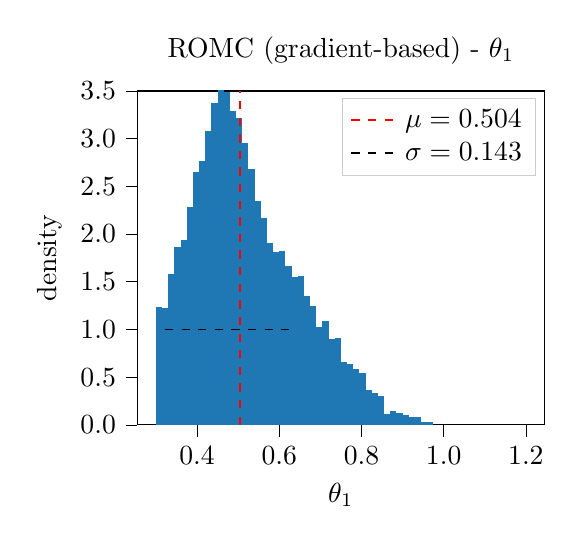
\begin{tikzpicture}

\definecolor{color0}{rgb}{0.12156862745098,0.466666666666667,0.705882352941177}

\begin{axis}[
legend cell align={left},
legend style={fill opacity=0.8, draw opacity=1, text opacity=1, draw=white!80!black},
tick align=outside,
tick pos=left,
title={ROMC (gradient-based) - \(\displaystyle \theta_1\)},
x grid style={white!69.0196078431373!black},
xlabel={\(\displaystyle \theta_1\)},
xmin=0.255, xmax=1.245,
xtick style={color=black},
xtick={0.2,0.4,0.6,0.8,1,1.2,1.4},
xticklabels={
  \(\displaystyle {0.2}\),
  \(\displaystyle {0.4}\),
  \(\displaystyle {0.6}\),
  \(\displaystyle {0.8}\),
  \(\displaystyle {1.0}\),
  \(\displaystyle {1.2}\),
  \(\displaystyle {1.4}\)
},
y grid style={white!69.0196078431373!black},
ylabel={density},
ymin=0, ymax=3.5,
ytick style={color=black},
ytick={0,0.5,1,1.5,2,2.5,3,3.5},
yticklabels={
  \(\displaystyle {0.0}\),
  \(\displaystyle {0.5}\),
  \(\displaystyle {1.0}\),
  \(\displaystyle {1.5}\),
  \(\displaystyle {2.0}\),
  \(\displaystyle {2.5}\),
  \(\displaystyle {3.0}\),
  \(\displaystyle {3.5}\)
}
]
\draw[draw=none,fill=color0] (axis cs:0.3,0) rectangle (axis cs:0.315,1.23969307221967);
\draw[draw=none,fill=color0] (axis cs:0.315,0) rectangle (axis cs:0.33,1.22260605418476);
\draw[draw=none,fill=color0] (axis cs:0.33,0) rectangle (axis cs:0.345,1.58099417689925);
\draw[draw=none,fill=color0] (axis cs:0.345,0) rectangle (axis cs:0.36,1.86697039022021);
\draw[draw=none,fill=color0] (axis cs:0.36,0) rectangle (axis cs:0.375,1.9327905830084);
\draw[draw=none,fill=color0] (axis cs:0.375,0) rectangle (axis cs:0.39,2.28560027755721);
\draw[draw=none,fill=color0] (axis cs:0.39,0) rectangle (axis cs:0.405,2.65528249842742);
\draw[draw=none,fill=color0] (axis cs:0.405,0) rectangle (axis cs:0.42,2.76542029517717);
\draw[draw=none,fill=color0] (axis cs:0.42,0) rectangle (axis cs:0.435,3.08006607906211);
\draw[draw=none,fill=color0] (axis cs:0.435,0) rectangle (axis cs:0.45,3.37496095644731);
\draw[draw=none,fill=color0] (axis cs:0.45,0) rectangle (axis cs:0.465,3.55021219168023);
\draw[draw=none,fill=color0] (axis cs:0.465,0) rectangle (axis cs:0.48,3.48979291667414);
\draw[draw=none,fill=color0] (axis cs:0.48,0) rectangle (axis cs:0.495,3.29497485978374);
\draw[draw=none,fill=color0] (axis cs:0.495,0) rectangle (axis cs:0.51,3.21369852560985);
\draw[draw=none,fill=color0] (axis cs:0.51,0) rectangle (axis cs:0.525,2.95263129250428);
\draw[draw=none,fill=color0] (axis cs:0.525,0) rectangle (axis cs:0.54,2.68186180204391);
\draw[draw=none,fill=color0] (axis cs:0.54,0) rectangle (axis cs:0.555,2.34177450679284);
\draw[draw=none,fill=color0] (axis cs:0.555,0) rectangle (axis cs:0.57,2.16665229531096);
\draw[draw=none,fill=color0] (axis cs:0.57,0) rectangle (axis cs:0.585,1.90550699050888);
\draw[draw=none,fill=color0] (axis cs:0.585,0) rectangle (axis cs:0.6,1.80681861350051);
\draw[draw=none,fill=color0] (axis cs:0.6,0) rectangle (axis cs:0.615,1.82068989944754);
\draw[draw=none,fill=color0] (axis cs:0.615,0) rectangle (axis cs:0.63,1.66308656575326);
\draw[draw=none,fill=color0] (axis cs:0.63,0) rectangle (axis cs:0.645,1.55350554347052);
\draw[draw=none,fill=color0] (axis cs:0.645,0) rectangle (axis cs:0.66,1.55706027108261);
\draw[draw=none,fill=color0] (axis cs:0.66,0) rectangle (axis cs:0.675,1.34606411506585);
\draw[draw=none,fill=color0] (axis cs:0.675,0) rectangle (axis cs:0.69,1.25058859381965);
\draw[draw=none,fill=color0] (axis cs:0.69,0) rectangle (axis cs:0.705,1.02541420681756);
\draw[draw=none,fill=color0] (axis cs:0.705,0) rectangle (axis cs:0.72,1.08883061316133);
\draw[draw=none,fill=color0] (axis cs:0.72,0) rectangle (axis cs:0.735,0.901026681844632);
\draw[draw=none,fill=color0] (axis cs:0.735,0) rectangle (axis cs:0.75,0.90959073604536);
\draw[draw=none,fill=color0] (axis cs:0.75,0) rectangle (axis cs:0.765,0.663388353950532);
\draw[draw=none,fill=color0] (axis cs:0.765,0) rectangle (axis cs:0.78,0.635304321110202);
\draw[draw=none,fill=color0] (axis cs:0.78,0) rectangle (axis cs:0.795,0.584894248497155);
\draw[draw=none,fill=color0] (axis cs:0.795,0) rectangle (axis cs:0.81,0.541909616027169);
\draw[draw=none,fill=color0] (axis cs:0.81,0) rectangle (axis cs:0.825,0.364723435432413);
\draw[draw=none,fill=color0] (axis cs:0.825,0) rectangle (axis cs:0.84,0.337243430980688);
\draw[draw=none,fill=color0] (axis cs:0.84,0) rectangle (axis cs:0.855,0.304888876342628);
\draw[draw=none,fill=color0] (axis cs:0.855,0) rectangle (axis cs:0.87,0.11082071864216);
\draw[draw=none,fill=color0] (axis cs:0.87,0) rectangle (axis cs:0.885,0.14353193766205);
\draw[draw=none,fill=color0] (axis cs:0.885,0) rectangle (axis cs:0.9,0.12562311229572);
\draw[draw=none,fill=color0] (axis cs:0.9,0) rectangle (axis cs:0.915,0.107714286929387);
\draw[draw=none,fill=color0] (axis cs:0.915,0) rectangle (axis cs:0.93,0.0820282878821482);
\draw[draw=none,fill=color0] (axis cs:0.93,0) rectangle (axis cs:0.945,0.0827149079075519);
\draw[draw=none,fill=color0] (axis cs:0.945,0) rectangle (axis cs:0.96,0.0269285717323464);
\draw[draw=none,fill=color0] (axis cs:0.96,0) rectangle (axis cs:0.975,0.0307869571533697);
\draw[draw=none,fill=color0] (axis cs:0.975,0) rectangle (axis cs:0.99,0);
\draw[draw=none,fill=color0] (axis cs:0.99,0) rectangle (axis cs:1.005,0);
\draw[draw=none,fill=color0] (axis cs:1.005,0) rectangle (axis cs:1.02,0);
\draw[draw=none,fill=color0] (axis cs:1.02,0) rectangle (axis cs:1.035,0);
\draw[draw=none,fill=color0] (axis cs:1.035,0) rectangle (axis cs:1.05,0);
\draw[draw=none,fill=color0] (axis cs:1.05,0) rectangle (axis cs:1.065,0);
\draw[draw=none,fill=color0] (axis cs:1.065,0) rectangle (axis cs:1.08,0);
\draw[draw=none,fill=color0] (axis cs:1.08,0) rectangle (axis cs:1.095,0);
\draw[draw=none,fill=color0] (axis cs:1.095,0) rectangle (axis cs:1.11,0);
\draw[draw=none,fill=color0] (axis cs:1.11,0) rectangle (axis cs:1.125,0);
\draw[draw=none,fill=color0] (axis cs:1.125,0) rectangle (axis cs:1.14,0);
\draw[draw=none,fill=color0] (axis cs:1.14,0) rectangle (axis cs:1.155,0);
\draw[draw=none,fill=color0] (axis cs:1.155,0) rectangle (axis cs:1.17,0);
\draw[draw=none,fill=color0] (axis cs:1.17,0) rectangle (axis cs:1.185,0);
\draw[draw=none,fill=color0] (axis cs:1.185,0) rectangle (axis cs:1.2,0);
\addplot [semithick, red, dashed]
table {%
0.50403516578119 0
0.50403516578119 3.5
};
\addlegendentry{$\mu = 0.504$}
\addplot [semithick, black, dashed]
table {%
0.321847690178847 1
0.637029674539771 1
};
\addlegendentry{$\sigma = 0.143$}
\end{axis}

\end{tikzpicture}

    }
    \resizebox{.24\columnwidth}{!}{%
      % This file was created with tikzplotlib v0.9.12.
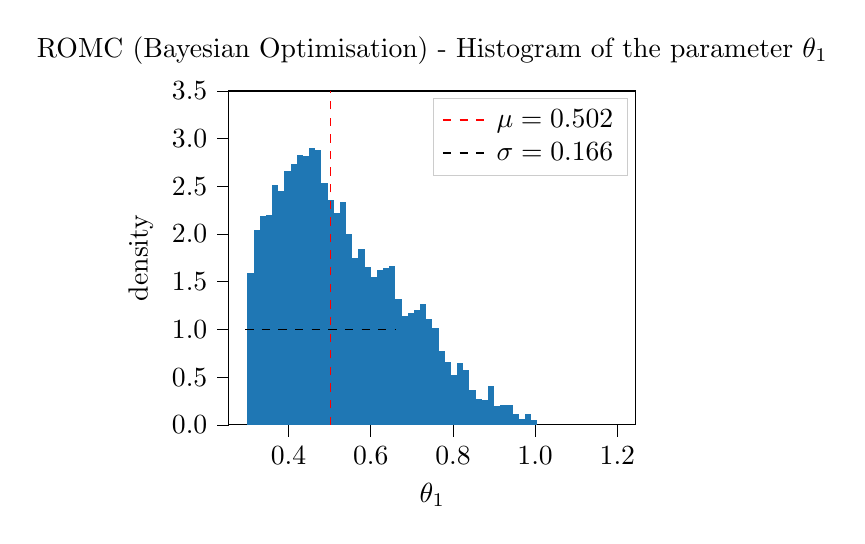
\begin{tikzpicture}

\definecolor{color0}{rgb}{0.12156862745098,0.466666666666667,0.705882352941177}

\begin{axis}[
legend cell align={left},
legend style={fill opacity=0.8, draw opacity=1, text opacity=1, draw=white!80!black},
tick align=outside,
tick pos=left,
title={ROMC (Bayesian Optimisation) - Histogram of the parameter \(\displaystyle \theta_1\)},
x grid style={white!69.0196078431373!black},
xlabel={\(\displaystyle \theta_1\)},
xmin=0.255, xmax=1.245,
xtick style={color=black},
xtick={0.2,0.4,0.6,0.8,1,1.2,1.4},
xticklabels={
  \(\displaystyle {0.2}\),
  \(\displaystyle {0.4}\),
  \(\displaystyle {0.6}\),
  \(\displaystyle {0.8}\),
  \(\displaystyle {1.0}\),
  \(\displaystyle {1.2}\),
  \(\displaystyle {1.4}\)
},
y grid style={white!69.0196078431373!black},
ylabel={density},
ymin=0, ymax=3.5,
ytick style={color=black},
ytick={0,0.5,1,1.5,2,2.5,3,3.5},
yticklabels={
  \(\displaystyle {0.0}\),
  \(\displaystyle {0.5}\),
  \(\displaystyle {1.0}\),
  \(\displaystyle {1.5}\),
  \(\displaystyle {2.0}\),
  \(\displaystyle {2.5}\),
  \(\displaystyle {3.0}\),
  \(\displaystyle {3.5}\)
}
]
\draw[draw=none,fill=color0] (axis cs:0.3,0) rectangle (axis cs:0.315,1.59230812208571);
\draw[draw=none,fill=color0] (axis cs:0.315,0) rectangle (axis cs:0.33,2.04310565145056);
\draw[draw=none,fill=color0] (axis cs:0.33,0) rectangle (axis cs:0.345,2.19382815490065);
\draw[draw=none,fill=color0] (axis cs:0.345,0) rectangle (axis cs:0.36,2.20021699441589);
\draw[draw=none,fill=color0] (axis cs:0.36,0) rectangle (axis cs:0.375,2.51506116421806);
\draw[draw=none,fill=color0] (axis cs:0.375,0) rectangle (axis cs:0.39,2.44880980882892);
\draw[draw=none,fill=color0] (axis cs:0.39,0) rectangle (axis cs:0.405,2.65904829491329);
\draw[draw=none,fill=color0] (axis cs:0.405,0) rectangle (axis cs:0.42,2.73250343027527);
\draw[draw=none,fill=color0] (axis cs:0.42,0) rectangle (axis cs:0.435,2.82852250487442);
\draw[draw=none,fill=color0] (axis cs:0.435,0) rectangle (axis cs:0.45,2.82331312648089);
\draw[draw=none,fill=color0] (axis cs:0.45,0) rectangle (axis cs:0.465,2.90135211837164);
\draw[draw=none,fill=color0] (axis cs:0.465,0) rectangle (axis cs:0.48,2.88136478592358);
\draw[draw=none,fill=color0] (axis cs:0.48,0) rectangle (axis cs:0.495,2.53560317010369);
\draw[draw=none,fill=color0] (axis cs:0.495,0) rectangle (axis cs:0.51,2.3564598017404);
\draw[draw=none,fill=color0] (axis cs:0.51,0) rectangle (axis cs:0.525,2.22420707945385);
\draw[draw=none,fill=color0] (axis cs:0.525,0) rectangle (axis cs:0.54,2.33534256536061);
\draw[draw=none,fill=color0] (axis cs:0.54,0) rectangle (axis cs:0.555,2.00495652659749);
\draw[draw=none,fill=color0] (axis cs:0.555,0) rectangle (axis cs:0.57,1.74992091039568);
\draw[draw=none,fill=color0] (axis cs:0.57,0) rectangle (axis cs:0.585,1.83870977452066);
\draw[draw=none,fill=color0] (axis cs:0.585,0) rectangle (axis cs:0.6,1.6578788920657);
\draw[draw=none,fill=color0] (axis cs:0.6,0) rectangle (axis cs:0.615,1.55026416918985);
\draw[draw=none,fill=color0] (axis cs:0.615,0) rectangle (axis cs:0.63,1.62152961093496);
\draw[draw=none,fill=color0] (axis cs:0.63,0) rectangle (axis cs:0.645,1.6437730803435);
\draw[draw=none,fill=color0] (axis cs:0.645,0) rectangle (axis cs:0.66,1.66640493128548);
\draw[draw=none,fill=color0] (axis cs:0.66,0) rectangle (axis cs:0.675,1.32365272171391);
\draw[draw=none,fill=color0] (axis cs:0.675,0) rectangle (axis cs:0.69,1.14155317519524);
\draw[draw=none,fill=color0] (axis cs:0.69,0) rectangle (axis cs:0.705,1.17480604967746);
\draw[draw=none,fill=color0] (axis cs:0.705,0) rectangle (axis cs:0.72,1.20896637137188);
\draw[draw=none,fill=color0] (axis cs:0.72,0) rectangle (axis cs:0.735,1.26617555858479);
\draw[draw=none,fill=color0] (axis cs:0.735,0) rectangle (axis cs:0.75,1.10815016078187);
\draw[draw=none,fill=color0] (axis cs:0.75,0) rectangle (axis cs:0.765,1.01575133068398);
\draw[draw=none,fill=color0] (axis cs:0.765,0) rectangle (axis cs:0.78,0.778653581806476);
\draw[draw=none,fill=color0] (axis cs:0.78,0) rectangle (axis cs:0.795,0.658517776017212);
\draw[draw=none,fill=color0] (axis cs:0.795,0) rectangle (axis cs:0.81,0.522857721601219);
\draw[draw=none,fill=color0] (axis cs:0.81,0) rectangle (axis cs:0.825,0.649384569447495);
\draw[draw=none,fill=color0] (axis cs:0.825,0) rectangle (axis cs:0.84,0.571069158563703);
\draw[draw=none,fill=color0] (axis cs:0.84,0) rectangle (axis cs:0.855,0.362376122626364);
\draw[draw=none,fill=color0] (axis cs:0.855,0) rectangle (axis cs:0.87,0.275087556542002);
\draw[draw=none,fill=color0] (axis cs:0.87,0) rectangle (axis cs:0.885,0.255847252846728);
\draw[draw=none,fill=color0] (axis cs:0.885,0) rectangle (axis cs:0.9,0.406941618766892);
\draw[draw=none,fill=color0] (axis cs:0.9,0) rectangle (axis cs:0.915,0.192257669195406);
\draw[draw=none,fill=color0] (axis cs:0.915,0) rectangle (axis cs:0.93,0.204927790769102);
\draw[draw=none,fill=color0] (axis cs:0.93,0) rectangle (axis cs:0.945,0.203525138747285);
\draw[draw=none,fill=color0] (axis cs:0.945,0) rectangle (axis cs:0.96,0.113584712363094);
\draw[draw=none,fill=color0] (axis cs:0.96,0) rectangle (axis cs:0.975,0.0662010640185658);
\draw[draw=none,fill=color0] (axis cs:0.975,0) rectangle (axis cs:0.99,0.116253091726246);
\draw[draw=none,fill=color0] (axis cs:0.99,0) rectangle (axis cs:1.005,0.0456418048890116);
\draw[draw=none,fill=color0] (axis cs:1.005,0) rectangle (axis cs:1.02,0);
\draw[draw=none,fill=color0] (axis cs:1.02,0) rectangle (axis cs:1.035,0);
\draw[draw=none,fill=color0] (axis cs:1.035,0) rectangle (axis cs:1.05,0);
\draw[draw=none,fill=color0] (axis cs:1.05,0) rectangle (axis cs:1.065,0);
\draw[draw=none,fill=color0] (axis cs:1.065,0) rectangle (axis cs:1.08,0);
\draw[draw=none,fill=color0] (axis cs:1.08,0) rectangle (axis cs:1.095,0);
\draw[draw=none,fill=color0] (axis cs:1.095,0) rectangle (axis cs:1.11,0);
\draw[draw=none,fill=color0] (axis cs:1.11,0) rectangle (axis cs:1.125,0);
\draw[draw=none,fill=color0] (axis cs:1.125,0) rectangle (axis cs:1.14,0);
\draw[draw=none,fill=color0] (axis cs:1.14,0) rectangle (axis cs:1.155,0);
\draw[draw=none,fill=color0] (axis cs:1.155,0) rectangle (axis cs:1.17,0);
\draw[draw=none,fill=color0] (axis cs:1.17,0) rectangle (axis cs:1.185,0);
\draw[draw=none,fill=color0] (axis cs:1.185,0) rectangle (axis cs:1.2,0);
\addplot [semithick, red, dashed]
table {%
0.502312841390367 0
0.502312841390367 3.5
};
\addlegendentry{$\mu = 0.502$}
\addplot [semithick, black, dashed]
table {%
0.294820390999603 1
0.660267860059204 1
};
\addlegendentry{$\sigma = 0.166$}
\end{axis}

\end{tikzpicture}

    }
    \resizebox{.24\columnwidth}{!}{%
      % This file was created with tikzplotlib v0.9.12.
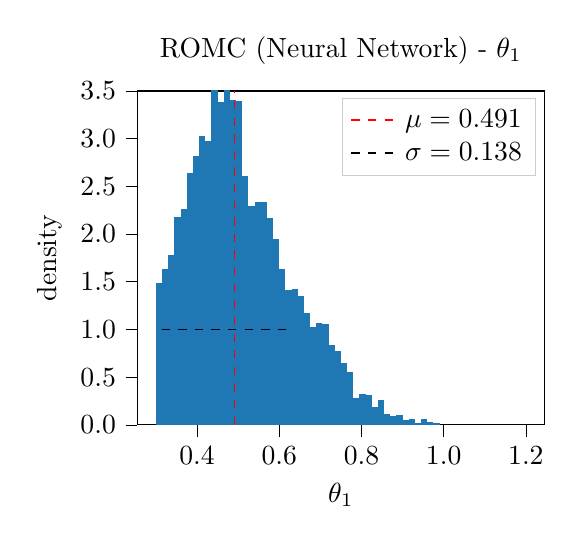
\begin{tikzpicture}

\definecolor{color0}{rgb}{0.12156862745098,0.466666666666667,0.705882352941177}

\begin{axis}[
legend cell align={left},
legend style={fill opacity=0.8, draw opacity=1, text opacity=1, draw=white!80!black},
tick align=outside,
tick pos=left,
title={ROMC (Neural Network) - \(\displaystyle \theta_1\)},
x grid style={white!69.0196078431373!black},
xlabel={\(\displaystyle \theta_1\)},
xmin=0.255, xmax=1.245,
xtick style={color=black},
xtick={0.2,0.4,0.6,0.8,1,1.2,1.4},
xticklabels={
  \(\displaystyle {0.2}\),
  \(\displaystyle {0.4}\),
  \(\displaystyle {0.6}\),
  \(\displaystyle {0.8}\),
  \(\displaystyle {1.0}\),
  \(\displaystyle {1.2}\),
  \(\displaystyle {1.4}\)
},
y grid style={white!69.0196078431373!black},
ylabel={density},
ymin=0, ymax=3.5,
ytick style={color=black},
ytick={0,0.5,1,1.5,2,2.5,3,3.5},
yticklabels={
  \(\displaystyle {0.0}\),
  \(\displaystyle {0.5}\),
  \(\displaystyle {1.0}\),
  \(\displaystyle {1.5}\),
  \(\displaystyle {2.0}\),
  \(\displaystyle {2.5}\),
  \(\displaystyle {3.0}\),
  \(\displaystyle {3.5}\)
}
]
\draw[draw=none,fill=color0] (axis cs:0.3,0) rectangle (axis cs:0.315,1.4847013386292);
\draw[draw=none,fill=color0] (axis cs:0.315,0) rectangle (axis cs:0.33,1.63008300744943);
\draw[draw=none,fill=color0] (axis cs:0.33,0) rectangle (axis cs:0.345,1.78269414852667);
\draw[draw=none,fill=color0] (axis cs:0.345,0) rectangle (axis cs:0.36,2.17914288457748);
\draw[draw=none,fill=color0] (axis cs:0.36,0) rectangle (axis cs:0.375,2.26619550399379);
\draw[draw=none,fill=color0] (axis cs:0.375,0) rectangle (axis cs:0.39,2.63578624756494);
\draw[draw=none,fill=color0] (axis cs:0.39,0) rectangle (axis cs:0.405,2.81808795446661);
\draw[draw=none,fill=color0] (axis cs:0.405,0) rectangle (axis cs:0.42,3.02972033457779);
\draw[draw=none,fill=color0] (axis cs:0.42,0) rectangle (axis cs:0.435,2.97861443343929);
\draw[draw=none,fill=color0] (axis cs:0.435,0) rectangle (axis cs:0.45,3.5112192843295);
\draw[draw=none,fill=color0] (axis cs:0.45,0) rectangle (axis cs:0.465,3.38441750293694);
\draw[draw=none,fill=color0] (axis cs:0.465,0) rectangle (axis cs:0.48,3.60452518165752);
\draw[draw=none,fill=color0] (axis cs:0.48,0) rectangle (axis cs:0.495,3.40496357685519);
\draw[draw=none,fill=color0] (axis cs:0.495,0) rectangle (axis cs:0.51,3.39267433638072);
\draw[draw=none,fill=color0] (axis cs:0.51,0) rectangle (axis cs:0.525,2.60955375534895);
\draw[draw=none,fill=color0] (axis cs:0.525,0) rectangle (axis cs:0.54,2.29229691711042);
\draw[draw=none,fill=color0] (axis cs:0.54,0) rectangle (axis cs:0.555,2.33810216344099);
\draw[draw=none,fill=color0] (axis cs:0.555,0) rectangle (axis cs:0.57,2.33307056573176);
\draw[draw=none,fill=color0] (axis cs:0.57,0) rectangle (axis cs:0.585,2.16876578921053);
\draw[draw=none,fill=color0] (axis cs:0.585,0) rectangle (axis cs:0.6,1.94786358717711);
\draw[draw=none,fill=color0] (axis cs:0.6,0) rectangle (axis cs:0.615,1.6348432484266);
\draw[draw=none,fill=color0] (axis cs:0.615,0) rectangle (axis cs:0.63,1.41781765326629);
\draw[draw=none,fill=color0] (axis cs:0.63,0) rectangle (axis cs:0.645,1.42854946707319);
\draw[draw=none,fill=color0] (axis cs:0.645,0) rectangle (axis cs:0.66,1.34821580131638);
\draw[draw=none,fill=color0] (axis cs:0.66,0) rectangle (axis cs:0.675,1.16914162978256);
\draw[draw=none,fill=color0] (axis cs:0.675,0) rectangle (axis cs:0.69,1.02253080695157);
\draw[draw=none,fill=color0] (axis cs:0.69,0) rectangle (axis cs:0.705,1.06697582017199);
\draw[draw=none,fill=color0] (axis cs:0.705,0) rectangle (axis cs:0.72,1.05900414126017);
\draw[draw=none,fill=color0] (axis cs:0.72,0) rectangle (axis cs:0.735,0.834884752208823);
\draw[draw=none,fill=color0] (axis cs:0.735,0) rectangle (axis cs:0.75,0.771804085452666);
\draw[draw=none,fill=color0] (axis cs:0.75,0) rectangle (axis cs:0.765,0.651009521206343);
\draw[draw=none,fill=color0] (axis cs:0.765,0) rectangle (axis cs:0.78,0.552051125172065);
\draw[draw=none,fill=color0] (axis cs:0.78,0) rectangle (axis cs:0.795,0.283364267425877);
\draw[draw=none,fill=color0] (axis cs:0.795,0) rectangle (axis cs:0.81,0.321951539666027);
\draw[draw=none,fill=color0] (axis cs:0.81,0) rectangle (axis cs:0.825,0.31247072638644);
\draw[draw=none,fill=color0] (axis cs:0.825,0) rectangle (axis cs:0.84,0.18976114249095);
\draw[draw=none,fill=color0] (axis cs:0.84,0) rectangle (axis cs:0.855,0.255316789610236);
\draw[draw=none,fill=color0] (axis cs:0.855,0) rectangle (axis cs:0.87,0.110079997689329);
\draw[draw=none,fill=color0] (axis cs:0.87,0) rectangle (axis cs:0.885,0.0946414093799529);
\draw[draw=none,fill=color0] (axis cs:0.885,0) rectangle (axis cs:0.9,0.104932268497323);
\draw[draw=none,fill=color0] (axis cs:0.9,0) rectangle (axis cs:0.915,0.0466365637765878);
\draw[draw=none,fill=color0] (axis cs:0.915,0) rectangle (axis cs:0.93,0.0582957047207339);
\draw[draw=none,fill=color0] (axis cs:0.93,0) rectangle (axis cs:0.945,0.0233182818882939);
\draw[draw=none,fill=color0] (axis cs:0.945,0) rectangle (axis cs:0.96,0.0582957047207339);
\draw[draw=none,fill=color0] (axis cs:0.96,0) rectangle (axis cs:0.975,0.0349774228324409);
\draw[draw=none,fill=color0] (axis cs:0.975,0) rectangle (axis cs:0.99,0.0233182818882936);
\draw[draw=none,fill=color0] (axis cs:0.99,0) rectangle (axis cs:1.005,0);
\draw[draw=none,fill=color0] (axis cs:1.005,0) rectangle (axis cs:1.02,0);
\draw[draw=none,fill=color0] (axis cs:1.02,0) rectangle (axis cs:1.035,0);
\draw[draw=none,fill=color0] (axis cs:1.035,0) rectangle (axis cs:1.05,0);
\draw[draw=none,fill=color0] (axis cs:1.05,0) rectangle (axis cs:1.065,0);
\draw[draw=none,fill=color0] (axis cs:1.065,0) rectangle (axis cs:1.08,0);
\draw[draw=none,fill=color0] (axis cs:1.08,0) rectangle (axis cs:1.095,0);
\draw[draw=none,fill=color0] (axis cs:1.095,0) rectangle (axis cs:1.11,0);
\draw[draw=none,fill=color0] (axis cs:1.11,0) rectangle (axis cs:1.125,0);
\draw[draw=none,fill=color0] (axis cs:1.125,0) rectangle (axis cs:1.14,0);
\draw[draw=none,fill=color0] (axis cs:1.14,0) rectangle (axis cs:1.155,0);
\draw[draw=none,fill=color0] (axis cs:1.155,0) rectangle (axis cs:1.17,0);
\draw[draw=none,fill=color0] (axis cs:1.17,0) rectangle (axis cs:1.185,0);
\draw[draw=none,fill=color0] (axis cs:1.185,0) rectangle (axis cs:1.2,0);
\addplot [semithick, red, dashed]
table {%
0.491475759372051 0
0.491475759372051 3.5
};
\addlegendentry{$\mu = 0.491$}
\addplot [semithick, black, dashed]
table {%
0.313768529672519 1
0.617478140945993 1
};
\addlegendentry{$\sigma = 0.138$}
\end{axis}

\end{tikzpicture}

    }\\
    \resizebox{.24\columnwidth}{!}{%
      \input{./latex_files/images/chapter4/mae2_hist_t2_rejection.tex}
    }
    \resizebox{.24\columnwidth}{!}{%
      % This file was created with tikzplotlib v0.9.12.
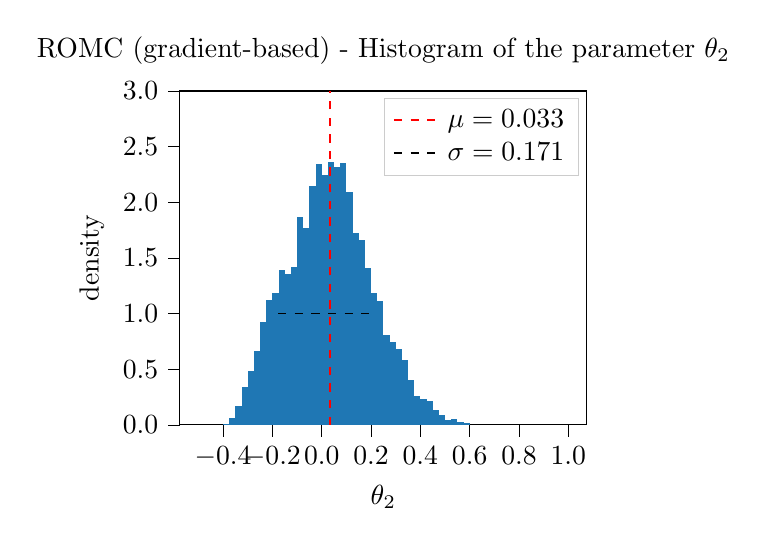
\begin{tikzpicture}

\definecolor{color0}{rgb}{0.12156862745098,0.466666666666667,0.705882352941177}

\begin{axis}[
legend cell align={left},
legend style={fill opacity=0.8, draw opacity=1, text opacity=1, draw=white!80!black},
tick align=outside,
tick pos=left,
title={ROMC (gradient-based) - Histogram of the parameter \(\displaystyle \theta_2\)},
x grid style={white!69.0196078431373!black},
xlabel={\(\displaystyle \theta_2\)},
xmin=-0.575, xmax=1.075,
xtick style={color=black},
xtick={-0.6,-0.4,-0.2,0,0.2,0.4,0.6,0.8,1,1.2},
xticklabels={
  \(\displaystyle {\ensuremath{-}0.6}\),
  \(\displaystyle {\ensuremath{-}0.4}\),
  \(\displaystyle {\ensuremath{-}0.2}\),
  \(\displaystyle {0.0}\),
  \(\displaystyle {0.2}\),
  \(\displaystyle {0.4}\),
  \(\displaystyle {0.6}\),
  \(\displaystyle {0.8}\),
  \(\displaystyle {1.0}\),
  \(\displaystyle {1.2}\)
},
y grid style={white!69.0196078431373!black},
ylabel={density},
ymin=0, ymax=3,
ytick style={color=black},
ytick={0,0.5,1,1.5,2,2.5,3},
yticklabels={
  \(\displaystyle {0.0}\),
  \(\displaystyle {0.5}\),
  \(\displaystyle {1.0}\),
  \(\displaystyle {1.5}\),
  \(\displaystyle {2.0}\),
  \(\displaystyle {2.5}\),
  \(\displaystyle {3.0}\)
}
]
\draw[draw=none,fill=color0] (axis cs:-0.5,0) rectangle (axis cs:-0.475,0);
\draw[draw=none,fill=color0] (axis cs:-0.475,0) rectangle (axis cs:-0.45,0);
\draw[draw=none,fill=color0] (axis cs:-0.45,0) rectangle (axis cs:-0.425,0);
\draw[draw=none,fill=color0] (axis cs:-0.425,0) rectangle (axis cs:-0.4,0);
\draw[draw=none,fill=color0] (axis cs:-0.4,0) rectangle (axis cs:-0.375,0.00554428884192465);
\draw[draw=none,fill=color0] (axis cs:-0.375,0) rectangle (axis cs:-0.35,0.0609051679887177);
\draw[draw=none,fill=color0] (axis cs:-0.35,0) rectangle (axis cs:-0.325,0.172932144280507);
\draw[draw=none,fill=color0] (axis cs:-0.325,0) rectangle (axis cs:-0.3,0.33874934889258);
\draw[draw=none,fill=color0] (axis cs:-0.3,0) rectangle (axis cs:-0.275,0.484235646321314);
\draw[draw=none,fill=color0] (axis cs:-0.275,0) rectangle (axis cs:-0.25,0.665208164482786);
\draw[draw=none,fill=color0] (axis cs:-0.25,0) rectangle (axis cs:-0.225,0.92463814505837);
\draw[draw=none,fill=color0] (axis cs:-0.225,0) rectangle (axis cs:-0.2,1.12139409849263);
\draw[draw=none,fill=color0] (axis cs:-0.2,0) rectangle (axis cs:-0.175,1.18629739177248);
\draw[draw=none,fill=color0] (axis cs:-0.175,0) rectangle (axis cs:-0.15,1.38911741112759);
\draw[draw=none,fill=color0] (axis cs:-0.15,0) rectangle (axis cs:-0.125,1.3586665597235);
\draw[draw=none,fill=color0] (axis cs:-0.125,0) rectangle (axis cs:-0.1,1.4168730451184);
\draw[draw=none,fill=color0] (axis cs:-0.1,0) rectangle (axis cs:-0.075,1.86440804043856);
\draw[draw=none,fill=color0] (axis cs:-0.075,0) rectangle (axis cs:-0.05,1.77193230571172);
\draw[draw=none,fill=color0] (axis cs:-0.05,0) rectangle (axis cs:-0.025,2.14800442101592);
\draw[draw=none,fill=color0] (axis cs:-0.025,0) rectangle (axis cs:0,2.34373098482187);
\draw[draw=none,fill=color0] (axis cs:0,0) rectangle (axis cs:0.025,2.24893542723874);
\draw[draw=none,fill=color0] (axis cs:0.025,0) rectangle (axis cs:0.05,2.36527262608105);
\draw[draw=none,fill=color0] (axis cs:0.05,0) rectangle (axis cs:0.0750000000000001,2.32011000423491);
\draw[draw=none,fill=color0] (axis cs:0.0750000000000001,0) rectangle (axis cs:0.1,2.35112752816106);
\draw[draw=none,fill=color0] (axis cs:0.1,0) rectangle (axis cs:0.125,2.09237672296862);
\draw[draw=none,fill=color0] (axis cs:0.125,0) rectangle (axis cs:0.15,1.72225524667604);
\draw[draw=none,fill=color0] (axis cs:0.15,0) rectangle (axis cs:0.175,1.65885907591305);
\draw[draw=none,fill=color0] (axis cs:0.175,0) rectangle (axis cs:0.2,1.4089028988961);
\draw[draw=none,fill=color0] (axis cs:0.2,0) rectangle (axis cs:0.225,1.18892677075576);
\draw[draw=none,fill=color0] (axis cs:0.225,0) rectangle (axis cs:0.25,1.11057927007035);
\draw[draw=none,fill=color0] (axis cs:0.25,0) rectangle (axis cs:0.275,0.808010795099994);
\draw[draw=none,fill=color0] (axis cs:0.275,0) rectangle (axis cs:0.3,0.746145310081448);
\draw[draw=none,fill=color0] (axis cs:0.3,0) rectangle (axis cs:0.325,0.68232985247479);
\draw[draw=none,fill=color0] (axis cs:0.325,0) rectangle (axis cs:0.35,0.586634734027065);
\draw[draw=none,fill=color0] (axis cs:0.35,0) rectangle (axis cs:0.375,0.400470451389202);
\draw[draw=none,fill=color0] (axis cs:0.375,0) rectangle (axis cs:0.4,0.259104715630191);
\draw[draw=none,fill=color0] (axis cs:0.4,0) rectangle (axis cs:0.425,0.230773630659991);
\draw[draw=none,fill=color0] (axis cs:0.425,0) rectangle (axis cs:0.45,0.211235556781049);
\draw[draw=none,fill=color0] (axis cs:0.45,0) rectangle (axis cs:0.475,0.129869421833243);
\draw[draw=none,fill=color0] (axis cs:0.475,0) rectangle (axis cs:0.5,0.0903839207491964);
\draw[draw=none,fill=color0] (axis cs:0.5,0) rectangle (axis cs:0.525,0.0434117816322698);
\draw[draw=none,fill=color0] (axis cs:0.525,0) rectangle (axis cs:0.55,0.0482353129247447);
\draw[draw=none,fill=color0] (axis cs:0.55,0) rectangle (axis cs:0.575,0.0289411877548468);
\draw[draw=none,fill=color0] (axis cs:0.575,0) rectangle (axis cs:0.6,0.0144705938774233);
\draw[draw=none,fill=color0] (axis cs:0.6,0) rectangle (axis cs:0.625,0);
\draw[draw=none,fill=color0] (axis cs:0.625,0) rectangle (axis cs:0.65,0);
\draw[draw=none,fill=color0] (axis cs:0.65,0) rectangle (axis cs:0.675,0);
\draw[draw=none,fill=color0] (axis cs:0.675,0) rectangle (axis cs:0.7,0);
\draw[draw=none,fill=color0] (axis cs:0.7,0) rectangle (axis cs:0.725,0);
\draw[draw=none,fill=color0] (axis cs:0.725,0) rectangle (axis cs:0.75,0);
\draw[draw=none,fill=color0] (axis cs:0.75,0) rectangle (axis cs:0.775,0);
\draw[draw=none,fill=color0] (axis cs:0.775,0) rectangle (axis cs:0.8,0);
\draw[draw=none,fill=color0] (axis cs:0.8,0) rectangle (axis cs:0.825,0);
\draw[draw=none,fill=color0] (axis cs:0.825,0) rectangle (axis cs:0.85,0);
\draw[draw=none,fill=color0] (axis cs:0.85,0) rectangle (axis cs:0.875,0);
\draw[draw=none,fill=color0] (axis cs:0.875,0) rectangle (axis cs:0.9,0);
\draw[draw=none,fill=color0] (axis cs:0.9,0) rectangle (axis cs:0.925,0);
\draw[draw=none,fill=color0] (axis cs:0.925,0) rectangle (axis cs:0.95,0);
\draw[draw=none,fill=color0] (axis cs:0.95,0) rectangle (axis cs:0.975,0);
\draw[draw=none,fill=color0] (axis cs:0.975,0) rectangle (axis cs:1,0);
\addplot [semithick, red, dashed]
table {%
0.0325607299281219 0
0.0325607299281219 3
};
\addlegendentry{$\mu = 0.033$}
\addplot [semithick, black, dashed]
table {%
-0.17677281465975 1
0.198406420501618 1
};
\addlegendentry{$\sigma = 0.171$}
\end{axis}

\end{tikzpicture}

    }
    \resizebox{.24\columnwidth}{!}{%
      % This file was created with tikzplotlib v0.9.12.
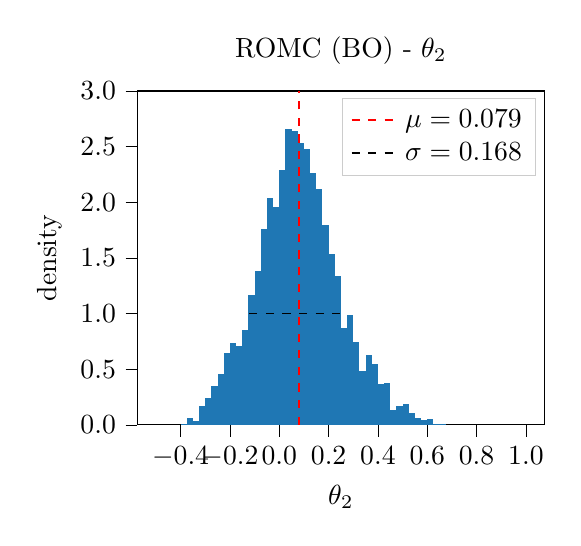
\begin{tikzpicture}

\definecolor{color0}{rgb}{0.12156862745098,0.466666666666667,0.705882352941177}

\begin{axis}[
legend cell align={left},
legend style={fill opacity=0.8, draw opacity=1, text opacity=1, draw=white!80!black},
tick align=outside,
tick pos=left,
title={ROMC (BO) - \(\displaystyle \theta_2\)},
x grid style={white!69.0196078431373!black},
xlabel={\(\displaystyle \theta_2\)},
xmin=-0.575, xmax=1.075,
xtick style={color=black},
xtick={-0.6,-0.4,-0.2,0,0.2,0.4,0.6,0.8,1,1.2},
xticklabels={
  \(\displaystyle {\ensuremath{-}0.6}\),
  \(\displaystyle {\ensuremath{-}0.4}\),
  \(\displaystyle {\ensuremath{-}0.2}\),
  \(\displaystyle {0.0}\),
  \(\displaystyle {0.2}\),
  \(\displaystyle {0.4}\),
  \(\displaystyle {0.6}\),
  \(\displaystyle {0.8}\),
  \(\displaystyle {1.0}\),
  \(\displaystyle {1.2}\)
},
y grid style={white!69.0196078431373!black},
ylabel={density},
ymin=0, ymax=3,
ytick style={color=black},
ytick={0,0.5,1,1.5,2,2.5,3},
yticklabels={
  \(\displaystyle {0.0}\),
  \(\displaystyle {0.5}\),
  \(\displaystyle {1.0}\),
  \(\displaystyle {1.5}\),
  \(\displaystyle {2.0}\),
  \(\displaystyle {2.5}\),
  \(\displaystyle {3.0}\)
}
]
\draw[draw=none,fill=color0] (axis cs:-0.5,0) rectangle (axis cs:-0.475,0);
\draw[draw=none,fill=color0] (axis cs:-0.475,0) rectangle (axis cs:-0.45,0);
\draw[draw=none,fill=color0] (axis cs:-0.45,0) rectangle (axis cs:-0.425,0);
\draw[draw=none,fill=color0] (axis cs:-0.425,0) rectangle (axis cs:-0.4,0);
\draw[draw=none,fill=color0] (axis cs:-0.4,0) rectangle (axis cs:-0.375,0.00425643655908195);
\draw[draw=none,fill=color0] (axis cs:-0.375,0) rectangle (axis cs:-0.35,0.0584436505421199);
\draw[draw=none,fill=color0] (axis cs:-0.35,0) rectangle (axis cs:-0.325,0.032329412084104);
\draw[draw=none,fill=color0] (axis cs:-0.325,0) rectangle (axis cs:-0.3,0.170488346927624);
\draw[draw=none,fill=color0] (axis cs:-0.3,0) rectangle (axis cs:-0.275,0.241312187040701);
\draw[draw=none,fill=color0] (axis cs:-0.275,0) rectangle (axis cs:-0.25,0.353203225767864);
\draw[draw=none,fill=color0] (axis cs:-0.25,0) rectangle (axis cs:-0.225,0.454783676389647);
\draw[draw=none,fill=color0] (axis cs:-0.225,0) rectangle (axis cs:-0.2,0.645870310110015);
\draw[draw=none,fill=color0] (axis cs:-0.2,0) rectangle (axis cs:-0.175,0.736855945766172);
\draw[draw=none,fill=color0] (axis cs:-0.175,0) rectangle (axis cs:-0.15,0.7054880882772);
\draw[draw=none,fill=color0] (axis cs:-0.15,0) rectangle (axis cs:-0.125,0.853720954547648);
\draw[draw=none,fill=color0] (axis cs:-0.125,0) rectangle (axis cs:-0.1,1.16488627133908);
\draw[draw=none,fill=color0] (axis cs:-0.1,0) rectangle (axis cs:-0.075,1.37944888929298);
\draw[draw=none,fill=color0] (axis cs:-0.075,0) rectangle (axis cs:-0.05,1.75863459008645);
\draw[draw=none,fill=color0] (axis cs:-0.05,0) rectangle (axis cs:-0.025,2.04186645728356);
\draw[draw=none,fill=color0] (axis cs:-0.025,0) rectangle (axis cs:0,1.95487930439736);
\draw[draw=none,fill=color0] (axis cs:0,0) rectangle (axis cs:0.025,2.2931926651875);
\draw[draw=none,fill=color0] (axis cs:0.025,0) rectangle (axis cs:0.05,2.65546746491156);
\draw[draw=none,fill=color0] (axis cs:0.05,0) rectangle (axis cs:0.0750000000000001,2.64247045528465);
\draw[draw=none,fill=color0] (axis cs:0.0750000000000001,0) rectangle (axis cs:0.1,2.53538619434107);
\draw[draw=none,fill=color0] (axis cs:0.1,0) rectangle (axis cs:0.125,2.47437216167486);
\draw[draw=none,fill=color0] (axis cs:0.125,0) rectangle (axis cs:0.15,2.25894133814364);
\draw[draw=none,fill=color0] (axis cs:0.15,0) rectangle (axis cs:0.175,2.12306099510411);
\draw[draw=none,fill=color0] (axis cs:0.175,0) rectangle (axis cs:0.2,1.79209215192117);
\draw[draw=none,fill=color0] (axis cs:0.2,0) rectangle (axis cs:0.225,1.53877177811189);
\draw[draw=none,fill=color0] (axis cs:0.225,0) rectangle (axis cs:0.25,1.34176813031492);
\draw[draw=none,fill=color0] (axis cs:0.25,0) rectangle (axis cs:0.275,0.869256102075021);
\draw[draw=none,fill=color0] (axis cs:0.275,0) rectangle (axis cs:0.3,0.984211536278622);
\draw[draw=none,fill=color0] (axis cs:0.3,0) rectangle (axis cs:0.325,0.744495637346589);
\draw[draw=none,fill=color0] (axis cs:0.325,0) rectangle (axis cs:0.35,0.487332826886714);
\draw[draw=none,fill=color0] (axis cs:0.35,0) rectangle (axis cs:0.375,0.631223471040121);
\draw[draw=none,fill=color0] (axis cs:0.375,0) rectangle (axis cs:0.4,0.5510631368371);
\draw[draw=none,fill=color0] (axis cs:0.4,0) rectangle (axis cs:0.425,0.369415701030125);
\draw[draw=none,fill=color0] (axis cs:0.425,0) rectangle (axis cs:0.45,0.376101401475276);
\draw[draw=none,fill=color0] (axis cs:0.45,0) rectangle (axis cs:0.475,0.135239439335051);
\draw[draw=none,fill=color0] (axis cs:0.475,0) rectangle (axis cs:0.5,0.17253048109158);
\draw[draw=none,fill=color0] (axis cs:0.5,0) rectangle (axis cs:0.525,0.187926500765093);
\draw[draw=none,fill=color0] (axis cs:0.525,0) rectangle (axis cs:0.55,0.106413103399642);
\draw[draw=none,fill=color0] (axis cs:0.55,0) rectangle (axis cs:0.575,0.0572991796412681);
\draw[draw=none,fill=color0] (axis cs:0.575,0) rectangle (axis cs:0.6,0.0435129826888125);
\draw[draw=none,fill=color0] (axis cs:0.6,0) rectangle (axis cs:0.625,0.0491139237583741);
\draw[draw=none,fill=color0] (axis cs:0.625,0) rectangle (axis cs:0.65,0.011416843630065);
\draw[draw=none,fill=color0] (axis cs:0.65,0) rectangle (axis cs:0.675,0.0114168436300651);
\draw[draw=none,fill=color0] (axis cs:0.675,0) rectangle (axis cs:0.7,3.98076835078974e-05);
\draw[draw=none,fill=color0] (axis cs:0.7,0) rectangle (axis cs:0.725,0);
\draw[draw=none,fill=color0] (axis cs:0.725,0) rectangle (axis cs:0.75,0);
\draw[draw=none,fill=color0] (axis cs:0.75,0) rectangle (axis cs:0.775,0);
\draw[draw=none,fill=color0] (axis cs:0.775,0) rectangle (axis cs:0.8,0);
\draw[draw=none,fill=color0] (axis cs:0.8,0) rectangle (axis cs:0.825,0);
\draw[draw=none,fill=color0] (axis cs:0.825,0) rectangle (axis cs:0.85,0);
\draw[draw=none,fill=color0] (axis cs:0.85,0) rectangle (axis cs:0.875,0);
\draw[draw=none,fill=color0] (axis cs:0.875,0) rectangle (axis cs:0.9,0);
\draw[draw=none,fill=color0] (axis cs:0.9,0) rectangle (axis cs:0.925,0);
\draw[draw=none,fill=color0] (axis cs:0.925,0) rectangle (axis cs:0.95,0);
\draw[draw=none,fill=color0] (axis cs:0.95,0) rectangle (axis cs:0.975,0);
\draw[draw=none,fill=color0] (axis cs:0.975,0) rectangle (axis cs:1,0);
\addplot [semithick, red, dashed]
table {%
0.0793529734576715 0
0.0793529734576715 3
};
\addlegendentry{$\mu = 0.079$}
\addplot [semithick, black, dashed]
table {%
-0.122023559466631 1
0.246600101073509 1
};
\addlegendentry{$\sigma = 0.168$}
\end{axis}

\end{tikzpicture}

    }
    \resizebox{.24\columnwidth}{!}{%
      % This file was created with tikzplotlib v0.9.12.
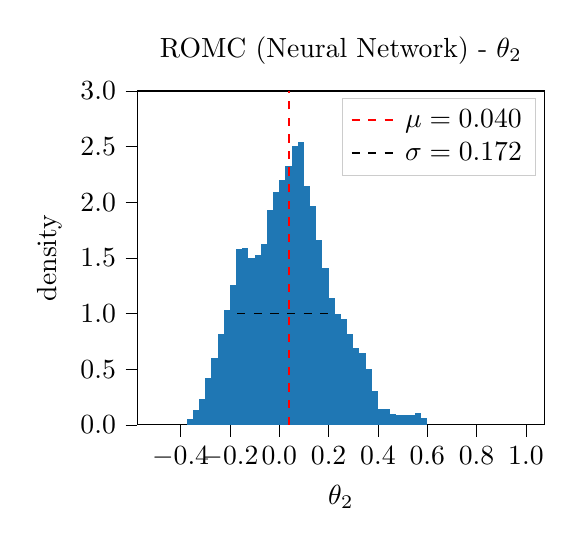
\begin{tikzpicture}

\definecolor{color0}{rgb}{0.12156862745098,0.466666666666667,0.705882352941177}

\begin{axis}[
legend cell align={left},
legend style={fill opacity=0.8, draw opacity=1, text opacity=1, draw=white!80!black},
tick align=outside,
tick pos=left,
title={ROMC (Neural Network) - \(\displaystyle \theta_2\)},
x grid style={white!69.0196078431373!black},
xlabel={\(\displaystyle \theta_2\)},
xmin=-0.575, xmax=1.075,
xtick style={color=black},
xtick={-0.6,-0.4,-0.2,0,0.2,0.4,0.6,0.8,1,1.2},
xticklabels={
  \(\displaystyle {\ensuremath{-}0.6}\),
  \(\displaystyle {\ensuremath{-}0.4}\),
  \(\displaystyle {\ensuremath{-}0.2}\),
  \(\displaystyle {0.0}\),
  \(\displaystyle {0.2}\),
  \(\displaystyle {0.4}\),
  \(\displaystyle {0.6}\),
  \(\displaystyle {0.8}\),
  \(\displaystyle {1.0}\),
  \(\displaystyle {1.2}\)
},
y grid style={white!69.0196078431373!black},
ylabel={density},
ymin=0, ymax=3,
ytick style={color=black},
ytick={0,0.5,1,1.5,2,2.5,3},
yticklabels={
  \(\displaystyle {0.0}\),
  \(\displaystyle {0.5}\),
  \(\displaystyle {1.0}\),
  \(\displaystyle {1.5}\),
  \(\displaystyle {2.0}\),
  \(\displaystyle {2.5}\),
  \(\displaystyle {3.0}\)
}
]
\draw[draw=none,fill=color0] (axis cs:-0.5,0) rectangle (axis cs:-0.475,0);
\draw[draw=none,fill=color0] (axis cs:-0.475,0) rectangle (axis cs:-0.45,0);
\draw[draw=none,fill=color0] (axis cs:-0.45,0) rectangle (axis cs:-0.425,0);
\draw[draw=none,fill=color0] (axis cs:-0.425,0) rectangle (axis cs:-0.4,0);
\draw[draw=none,fill=color0] (axis cs:-0.4,0) rectangle (axis cs:-0.375,0);
\draw[draw=none,fill=color0] (axis cs:-0.375,0) rectangle (axis cs:-0.35,0.0557676847180302);
\draw[draw=none,fill=color0] (axis cs:-0.35,0) rectangle (axis cs:-0.325,0.134391393873674);
\draw[draw=none,fill=color0] (axis cs:-0.325,0) rectangle (axis cs:-0.3,0.232670307676795);
\draw[draw=none,fill=color0] (axis cs:-0.3,0) rectangle (axis cs:-0.275,0.421300598168856);
\draw[draw=none,fill=color0] (axis cs:-0.275,0) rectangle (axis cs:-0.25,0.599565962284508);
\draw[draw=none,fill=color0] (axis cs:-0.25,0) rectangle (axis cs:-0.225,0.819487590375745);
\draw[draw=none,fill=color0] (axis cs:-0.225,0) rectangle (axis cs:-0.2,1.02995995908051);
\draw[draw=none,fill=color0] (axis cs:-0.2,0) rectangle (axis cs:-0.175,1.25665578855782);
\draw[draw=none,fill=color0] (axis cs:-0.175,0) rectangle (axis cs:-0.15,1.57888096147667);
\draw[draw=none,fill=color0] (axis cs:-0.15,0) rectangle (axis cs:-0.125,1.58957701821668);
\draw[draw=none,fill=color0] (axis cs:-0.125,0) rectangle (axis cs:-0.1,1.49600073368982);
\draw[draw=none,fill=color0] (axis cs:-0.1,0) rectangle (axis cs:-0.075,1.52507821911024);
\draw[draw=none,fill=color0] (axis cs:-0.075,0) rectangle (axis cs:-0.05,1.62625669151916);
\draw[draw=none,fill=color0] (axis cs:-0.05,0) rectangle (axis cs:-0.025,1.92752590520997);
\draw[draw=none,fill=color0] (axis cs:-0.025,0) rectangle (axis cs:0,2.09127677525018);
\draw[draw=none,fill=color0] (axis cs:0,0) rectangle (axis cs:0.025,2.20245981684059);
\draw[draw=none,fill=color0] (axis cs:0.025,0) rectangle (axis cs:0.05,2.32191116112789);
\draw[draw=none,fill=color0] (axis cs:0.05,0) rectangle (axis cs:0.0750000000000001,2.50351769805879);
\draw[draw=none,fill=color0] (axis cs:0.0750000000000001,0) rectangle (axis cs:0.1,2.54297681090209);
\draw[draw=none,fill=color0] (axis cs:0.1,0) rectangle (axis cs:0.125,2.14701105787528);
\draw[draw=none,fill=color0] (axis cs:0.125,0) rectangle (axis cs:0.15,1.97050861768377);
\draw[draw=none,fill=color0] (axis cs:0.15,0) rectangle (axis cs:0.175,1.65952774547258);
\draw[draw=none,fill=color0] (axis cs:0.175,0) rectangle (axis cs:0.2,1.41333954655085);
\draw[draw=none,fill=color0] (axis cs:0.2,0) rectangle (axis cs:0.225,1.1362319294878);
\draw[draw=none,fill=color0] (axis cs:0.225,0) rectangle (axis cs:0.25,0.992545439733498);
\draw[draw=none,fill=color0] (axis cs:0.25,0) rectangle (axis cs:0.275,0.95508724072649);
\draw[draw=none,fill=color0] (axis cs:0.275,0) rectangle (axis cs:0.3,0.820509887123889);
\draw[draw=none,fill=color0] (axis cs:0.3,0) rectangle (axis cs:0.325,0.693510954529521);
\draw[draw=none,fill=color0] (axis cs:0.325,0) rectangle (axis cs:0.35,0.644349818384951);
\draw[draw=none,fill=color0] (axis cs:0.35,0) rectangle (axis cs:0.375,0.49941685245109);
\draw[draw=none,fill=color0] (axis cs:0.375,0) rectangle (axis cs:0.4,0.304905545384957);
\draw[draw=none,fill=color0] (axis cs:0.4,0) rectangle (axis cs:0.425,0.137853649275808);
\draw[draw=none,fill=color0] (axis cs:0.425,0) rectangle (axis cs:0.45,0.144181418842862);
\draw[draw=none,fill=color0] (axis cs:0.45,0) rectangle (axis cs:0.475,0.0965680200621962);
\draw[draw=none,fill=color0] (axis cs:0.475,0) rectangle (axis cs:0.5,0.0871794625561498);
\draw[draw=none,fill=color0] (axis cs:0.5,0) rectangle (axis cs:0.525,0.087179462556149);
\draw[draw=none,fill=color0] (axis cs:0.525,0) rectangle (axis cs:0.55,0.0871794625561498);
\draw[draw=none,fill=color0] (axis cs:0.55,0) rectangle (axis cs:0.575,0.107297800069107);
\draw[draw=none,fill=color0] (axis cs:0.575,0) rectangle (axis cs:0.6,0.0603550125388724);
\draw[draw=none,fill=color0] (axis cs:0.6,0) rectangle (axis cs:0.625,0);
\draw[draw=none,fill=color0] (axis cs:0.625,0) rectangle (axis cs:0.65,0);
\draw[draw=none,fill=color0] (axis cs:0.65,0) rectangle (axis cs:0.675,0);
\draw[draw=none,fill=color0] (axis cs:0.675,0) rectangle (axis cs:0.7,0);
\draw[draw=none,fill=color0] (axis cs:0.7,0) rectangle (axis cs:0.725,0);
\draw[draw=none,fill=color0] (axis cs:0.725,0) rectangle (axis cs:0.75,0);
\draw[draw=none,fill=color0] (axis cs:0.75,0) rectangle (axis cs:0.775,0);
\draw[draw=none,fill=color0] (axis cs:0.775,0) rectangle (axis cs:0.8,0);
\draw[draw=none,fill=color0] (axis cs:0.8,0) rectangle (axis cs:0.825,0);
\draw[draw=none,fill=color0] (axis cs:0.825,0) rectangle (axis cs:0.85,0);
\draw[draw=none,fill=color0] (axis cs:0.85,0) rectangle (axis cs:0.875,0);
\draw[draw=none,fill=color0] (axis cs:0.875,0) rectangle (axis cs:0.9,0);
\draw[draw=none,fill=color0] (axis cs:0.9,0) rectangle (axis cs:0.925,0);
\draw[draw=none,fill=color0] (axis cs:0.925,0) rectangle (axis cs:0.95,0);
\draw[draw=none,fill=color0] (axis cs:0.95,0) rectangle (axis cs:0.975,0);
\draw[draw=none,fill=color0] (axis cs:0.975,0) rectangle (axis cs:1,0);
\addplot [semithick, red, dashed]
table {%
0.0396457758194439 0
0.0396457758194439 3
};
\addlegendentry{$\mu = 0.040$}
\addplot [semithick, black, dashed]
table {%
-0.170712448191162 1
0.207933154993939 1
};
\addlegendentry{$\sigma = 0.172$}
\end{axis}

\end{tikzpicture}

    }
    \end{center}
    \caption[MA2 example, evaluation of the marginal
    distributions.]{Histogram of the marginal posterior distributions
      using three different inference approaches; (a) in the first
      row, the samples are obtained using Rejection ABC sampling (b)
      in the second row, using ROMC with a gradient-based optimiser
      and (c) in the third row, using ROMC with Bayesian optimisation
      approach. The vertical (red) line represents the samples mean
      \(\mu\) and the horizontal (black) the standard deviation
      \(\sigma\).}
  \label{fig:ma2_3}
\end{figure}

\begin{figure}[ht]
  \begin{center}
    \resizebox{.32\columnwidth}{!}{%
      % This file was created with tikzplotlib v0.9.12.
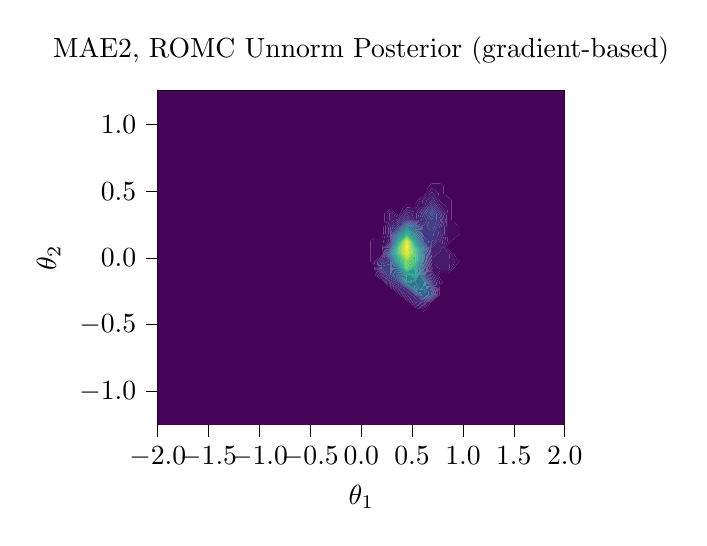
\begin{tikzpicture}

\definecolor{color0}{rgb}{0.269944,0.014625,0.341379}
\definecolor{color1}{rgb}{0.276022,0.044167,0.370164}
\definecolor{color2}{rgb}{0.280267,0.073417,0.397163}
\definecolor{color3}{rgb}{0.282656,0.100196,0.42216}
\definecolor{color4}{rgb}{0.283072,0.130895,0.449241}
\definecolor{color5}{rgb}{0.281412,0.155834,0.469201}
\definecolor{color6}{rgb}{0.278012,0.180367,0.486697}
\definecolor{color7}{rgb}{0.273006,0.20452,0.501721}
\definecolor{color8}{rgb}{0.26658,0.228262,0.514349}
\definecolor{color9}{rgb}{0.258965,0.251537,0.524736}
\definecolor{color10}{rgb}{0.250425,0.27429,0.533103}
\definecolor{color11}{rgb}{0.241237,0.296485,0.539709}
\definecolor{color12}{rgb}{0.229739,0.322361,0.545706}
\definecolor{color13}{rgb}{0.220057,0.343307,0.549413}
\definecolor{color14}{rgb}{0.210503,0.363727,0.552206}
\definecolor{color15}{rgb}{0.201239,0.38367,0.554294}
\definecolor{color16}{rgb}{0.192357,0.403199,0.555836}
\definecolor{color17}{rgb}{0.183898,0.422383,0.556944}
\definecolor{color18}{rgb}{0.175841,0.44129,0.557685}
\definecolor{color19}{rgb}{0.168126,0.459988,0.558082}
\definecolor{color20}{rgb}{0.160665,0.47854,0.558115}
\definecolor{color21}{rgb}{0.151918,0.500685,0.557587}
\definecolor{color22}{rgb}{0.144759,0.519093,0.556572}
\definecolor{color23}{rgb}{0.13777,0.537492,0.554906}
\definecolor{color24}{rgb}{0.131172,0.555899,0.552459}
\definecolor{color25}{rgb}{0.125394,0.574318,0.549086}
\definecolor{color26}{rgb}{0.121148,0.592739,0.544641}
\definecolor{color27}{rgb}{0.119423,0.611141,0.538982}
\definecolor{color28}{rgb}{0.12138,0.629492,0.531973}
\definecolor{color29}{rgb}{0.130067,0.651384,0.521608}
\definecolor{color30}{rgb}{0.143303,0.669459,0.511215}
\definecolor{color31}{rgb}{0.162016,0.687316,0.499129}
\definecolor{color32}{rgb}{0.185783,0.704891,0.485273}
\definecolor{color33}{rgb}{0.214,0.722114,0.469588}
\definecolor{color34}{rgb}{0.24607,0.73891,0.452024}
\definecolor{color35}{rgb}{0.281477,0.755203,0.432552}
\definecolor{color36}{rgb}{0.319809,0.770914,0.411152}
\definecolor{color37}{rgb}{0.369214,0.788888,0.382914}
\definecolor{color38}{rgb}{0.412913,0.803041,0.357269}
\definecolor{color39}{rgb}{0.458674,0.816363,0.329727}
\definecolor{color40}{rgb}{0.506271,0.828786,0.300362}
\definecolor{color41}{rgb}{0.555484,0.840254,0.269281}
\definecolor{color42}{rgb}{0.606045,0.850733,0.236712}
\definecolor{color43}{rgb}{0.657642,0.860219,0.203082}
\definecolor{color44}{rgb}{0.709898,0.868751,0.169257}
\definecolor{color45}{rgb}{0.762373,0.876424,0.137064}
\definecolor{color46}{rgb}{0.82494,0.88472,0.106217}
\definecolor{color47}{rgb}{0.876168,0.891125,0.09525}
\definecolor{color48}{rgb}{0.926106,0.89733,0.104071}
\definecolor{color49}{rgb}{0.974417,0.90359,0.130215}

\begin{axis}[
tick align=outside,
tick pos=left,
title={MAE2, ROMC Unnorm Posterior (gradient-based)},
x grid style={white!69.0196078431373!black},
xlabel={\(\displaystyle \theta_1\)},
xmin=-2, xmax=2,
xtick style={color=black},
xtick={-2,-1.5,-1,-0.5,0,0.5,1,1.5,2},
xticklabels={
  \(\displaystyle {\ensuremath{-}2.0}\),
  \(\displaystyle {\ensuremath{-}1.5}\),
  \(\displaystyle {\ensuremath{-}1.0}\),
  \(\displaystyle {\ensuremath{-}0.5}\),
  \(\displaystyle {0.0}\),
  \(\displaystyle {0.5}\),
  \(\displaystyle {1.0}\),
  \(\displaystyle {1.5}\),
  \(\displaystyle {2.0}\)
},
y grid style={white!69.0196078431373!black},
ylabel={\(\displaystyle \theta_2\)},
ymin=-1.25, ymax=1.25,
ytick style={color=black},
ytick={-1.5,-1,-0.5,0,0.5,1,1.5},
yticklabels={
  \(\displaystyle {\ensuremath{-}1.5}\),
  \(\displaystyle {\ensuremath{-}1.0}\),
  \(\displaystyle {\ensuremath{-}0.5}\),
  \(\displaystyle {0.0}\),
  \(\displaystyle {0.5}\),
  \(\displaystyle {1.0}\),
  \(\displaystyle {1.5}\)
}
]
\addplot [draw=none, fill=color0]
table{%
x  y
-1.91836734693878 -1.25
-1.83673469387755 -1.25
-1.75510204081633 -1.25
-1.6734693877551 -1.25
-1.59183673469388 -1.25
-1.51020408163265 -1.25
-1.42857142857143 -1.25
-1.3469387755102 -1.25
-1.26530612244898 -1.25
-1.18367346938776 -1.25
-1.10204081632653 -1.25
-1.02040816326531 -1.25
-0.938775510204082 -1.25
-0.857142857142857 -1.25
-0.775510204081633 -1.25
-0.693877551020408 -1.25
-0.612244897959184 -1.25
-0.530612244897959 -1.25
-0.448979591836735 -1.25
-0.36734693877551 -1.25
-0.285714285714286 -1.25
-0.204081632653061 -1.25
-0.122448979591837 -1.25
-0.0408163265306123 -1.25
0.0408163265306123 -1.25
0.122448979591836 -1.25
0.204081632653061 -1.25
0.285714285714286 -1.25
0.36734693877551 -1.25
0.448979591836734 -1.25
0.530612244897959 -1.25
0.612244897959183 -1.25
0.693877551020408 -1.25
0.775510204081633 -1.25
0.857142857142857 -1.25
0.938775510204081 -1.25
1.02040816326531 -1.25
1.10204081632653 -1.25
1.18367346938775 -1.25
1.26530612244898 -1.25
1.3469387755102 -1.25
1.42857142857143 -1.25
1.51020408163265 -1.25
1.59183673469388 -1.25
1.6734693877551 -1.25
1.75510204081633 -1.25
1.83673469387755 -1.25
1.91836734693878 -1.25
2 -1.25
2 -1.19897959183673
2 -1.14795918367347
2 -1.0969387755102
2 -1.04591836734694
2 -0.994897959183674
2 -0.943877551020408
2 -0.892857142857143
2 -0.841836734693878
2 -0.790816326530612
2 -0.739795918367347
2 -0.688775510204082
2 -0.637755102040816
2 -0.586734693877551
2 -0.535714285714286
2 -0.48469387755102
2 -0.433673469387755
2 -0.38265306122449
2 -0.331632653061224
2 -0.280612244897959
2 -0.229591836734694
2 -0.178571428571429
2 -0.127551020408163
2 -0.0765306122448979
2 -0.0255102040816326
2 0.0255102040816326
2 0.0765306122448979
2 0.127551020408163
2 0.178571428571429
2 0.229591836734694
2 0.280612244897959
2 0.331632653061225
2 0.38265306122449
2 0.433673469387755
2 0.48469387755102
2 0.535714285714286
2 0.586734693877551
2 0.637755102040816
2 0.688775510204082
2 0.739795918367347
2 0.790816326530612
2 0.841836734693878
2 0.892857142857143
2 0.943877551020408
2 0.994897959183674
2 1.04591836734694
2 1.0969387755102
2 1.14795918367347
2 1.19897959183673
2 1.25
1.91836734693878 1.25
1.83673469387755 1.25
1.75510204081633 1.25
1.6734693877551 1.25
1.59183673469388 1.25
1.51020408163265 1.25
1.42857142857143 1.25
1.3469387755102 1.25
1.26530612244898 1.25
1.18367346938775 1.25
1.10204081632653 1.25
1.02040816326531 1.25
0.938775510204081 1.25
0.857142857142857 1.25
0.775510204081633 1.25
0.693877551020408 1.25
0.612244897959183 1.25
0.530612244897959 1.25
0.448979591836734 1.25
0.36734693877551 1.25
0.285714285714286 1.25
0.204081632653061 1.25
0.122448979591836 1.25
0.0408163265306123 1.25
-0.0408163265306123 1.25
-0.122448979591837 1.25
-0.204081632653061 1.25
-0.285714285714286 1.25
-0.36734693877551 1.25
-0.448979591836735 1.25
-0.530612244897959 1.25
-0.612244897959184 1.25
-0.693877551020408 1.25
-0.775510204081633 1.25
-0.857142857142857 1.25
-0.938775510204082 1.25
-1.02040816326531 1.25
-1.10204081632653 1.25
-1.18367346938776 1.25
-1.26530612244898 1.25
-1.3469387755102 1.25
-1.42857142857143 1.25
-1.51020408163265 1.25
-1.59183673469388 1.25
-1.6734693877551 1.25
-1.75510204081633 1.25
-1.83673469387755 1.25
-1.91836734693878 1.25
-2 1.25
-2 1.19897959183673
-2 1.14795918367347
-2 1.0969387755102
-2 1.04591836734694
-2 0.994897959183674
-2 0.943877551020408
-2 0.892857142857143
-2 0.841836734693878
-2 0.790816326530612
-2 0.739795918367347
-2 0.688775510204082
-2 0.637755102040816
-2 0.586734693877551
-2 0.535714285714286
-2 0.48469387755102
-2 0.433673469387755
-2 0.38265306122449
-2 0.331632653061225
-2 0.280612244897959
-2 0.229591836734694
-2 0.178571428571429
-2 0.127551020408163
-2 0.0765306122448979
-2 0.0255102040816326
-2 -0.0255102040816326
-2 -0.0765306122448979
-2 -0.127551020408163
-2 -0.178571428571429
-2 -0.229591836734694
-2 -0.280612244897959
-2 -0.331632653061224
-2 -0.38265306122449
-2 -0.433673469387755
-2 -0.48469387755102
-2 -0.535714285714286
-2 -0.586734693877551
-2 -0.637755102040816
-2 -0.688775510204082
-2 -0.739795918367347
-2 -0.790816326530612
-2 -0.841836734693878
-2 -0.892857142857143
-2 -0.943877551020408
-2 -0.994897959183674
-2 -1.04591836734694
-2 -1.0969387755102
-2 -1.14795918367347
-2 -1.19897959183673
-2 -1.25
-1.91836734693878 -1.25

0.579591836734694 -0.38265306122449
0.530612244897959 -0.372448979591837
0.465306122448979 -0.331632653061224
0.448979591836734 -0.321428571428571
0.383673469387755 -0.280612244897959
0.36734693877551 -0.270408163265306
0.302040816326531 -0.229591836734694
0.285714285714286 -0.221938775510204
0.216326530612245 -0.178571428571429
0.204081632653061 -0.168367346938776
0.138775510204081 -0.127551020408163
0.130612244897959 -0.0765306122448979
0.122448979591836 -0.0459183673469387
0.0897959183673468 -0.0255102040816326
0.0897959183673468 0.0255102040816326
0.0897959183673468 0.0765306122448979
0.0897959183673468 0.127551020408163
0.122448979591836 0.147959183673469
0.204081632653061 0.147959183673469
0.220408163265306 0.178571428571429
0.220408163265306 0.229591836734694
0.228571428571428 0.280612244897959
0.228571428571428 0.331632653061225
0.285714285714286 0.36734693877551
0.342857142857143 0.331632653061225
0.36734693877551 0.321428571428572
0.383673469387755 0.331632653061225
0.416326530612245 0.38265306122449
0.448979591836734 0.403061224489796
0.530612244897959 0.403061224489796
0.555102040816326 0.433673469387755
0.612244897959183 0.469387755102041
0.636734693877551 0.48469387755102
0.661224489795918 0.535714285714286
0.693877551020408 0.556122448979592
0.775510204081633 0.556122448979592
0.808163265306122 0.535714285714286
0.808163265306122 0.48469387755102
0.857142857142857 0.454081632653061
0.889795918367347 0.433673469387755
0.889795918367347 0.38265306122449
0.889795918367347 0.331632653061225
0.889795918367347 0.280612244897959
0.938775510204081 0.25
0.971428571428571 0.229591836734694
0.971428571428571 0.178571428571429
0.938775510204081 0.158163265306123
0.889795918367347 0.127551020408163
0.857142857142857 0.107142857142857
0.840816326530612 0.0765306122448979
0.857142857142857 0.0612244897959183
0.914285714285714 0.0255102040816326
0.938775510204081 -0.00510204081632653
0.971428571428571 -0.0255102040816326
0.938775510204081 -0.0459183673469387
0.914285714285714 -0.0765306122448979
0.857142857142857 -0.112244897959184
0.775510204081633 -0.112244897959184
0.759183673469388 -0.127551020408163
0.775510204081633 -0.158163265306122
0.808163265306122 -0.178571428571429
0.775510204081633 -0.198979591836735
0.768513119533528 -0.229591836734694
0.769387755102041 -0.280612244897959
0.693877551020408 -0.32780612244898
0.681632653061224 -0.331632653061224
0.644897959183673 -0.38265306122449
0.612244897959183 -0.403061224489796
0.579591836734694 -0.38265306122449
};
\addplot [draw=none, fill=color1]
table{%
x  y
0.612244897959183 -0.403061224489796
0.644897959183673 -0.38265306122449
0.681632653061224 -0.331632653061224
0.693877551020408 -0.32780612244898
0.769387755102041 -0.280612244897959
0.768513119533528 -0.229591836734694
0.775510204081633 -0.198979591836735
0.808163265306122 -0.178571428571429
0.775510204081633 -0.158163265306122
0.759183673469388 -0.127551020408163
0.775510204081633 -0.112244897959184
0.857142857142857 -0.112244897959184
0.914285714285714 -0.0765306122448979
0.938775510204081 -0.0459183673469387
0.971428571428571 -0.0255102040816326
0.938775510204081 -0.00510204081632653
0.914285714285714 0.0255102040816326
0.857142857142857 0.0612244897959183
0.840816326530612 0.0765306122448979
0.857142857142857 0.107142857142857
0.889795918367347 0.127551020408163
0.938775510204081 0.158163265306123
0.971428571428571 0.178571428571429
0.971428571428571 0.229591836734694
0.938775510204081 0.25
0.889795918367347 0.280612244897959
0.889795918367347 0.331632653061225
0.889795918367347 0.38265306122449
0.889795918367347 0.433673469387755
0.857142857142857 0.454081632653061
0.808163265306122 0.48469387755102
0.808163265306122 0.535714285714286
0.775510204081633 0.556122448979592
0.693877551020408 0.556122448979592
0.661224489795918 0.535714285714286
0.636734693877551 0.48469387755102
0.612244897959183 0.469387755102041
0.555102040816326 0.433673469387755
0.530612244897959 0.403061224489796
0.448979591836734 0.403061224489796
0.416326530612245 0.38265306122449
0.383673469387755 0.331632653061225
0.36734693877551 0.321428571428572
0.342857142857143 0.331632653061225
0.285714285714286 0.36734693877551
0.228571428571428 0.331632653061225
0.228571428571428 0.280612244897959
0.220408163265306 0.229591836734694
0.220408163265306 0.178571428571429
0.204081632653061 0.147959183673469
0.122448979591836 0.147959183673469
0.0897959183673468 0.127551020408163
0.0897959183673468 0.0765306122448979
0.0897959183673468 0.0255102040816326
0.0897959183673468 -0.0255102040816326
0.122448979591836 -0.0459183673469387
0.130612244897959 -0.0765306122448979
0.138775510204081 -0.127551020408163
0.204081632653061 -0.168367346938776
0.216326530612245 -0.178571428571429
0.285714285714286 -0.221938775510204
0.302040816326531 -0.229591836734694
0.36734693877551 -0.270408163265306
0.383673469387755 -0.280612244897959
0.448979591836734 -0.321428571428571
0.465306122448979 -0.331632653061224
0.530612244897959 -0.372448979591837
0.579591836734694 -0.38265306122449
0.612244897959183 -0.403061224489796

0.481632653061224 -0.331632653061224
0.448979591836734 -0.311224489795918
0.4 -0.280612244897959
0.36734693877551 -0.260204081632653
0.318367346938775 -0.229591836734694
0.285714285714286 -0.214285714285714
0.228571428571428 -0.178571428571429
0.204081632653061 -0.158163265306122
0.155102040816326 -0.127551020408163
0.138775510204081 -0.0765306122448979
0.127891156462585 -0.0255102040816326
0.204081632653061 0.0221088435374149
0.205895691609977 0.0255102040816326
0.20734693877551 0.0765306122448979
0.220408163265306 0.127551020408163
0.236734693877551 0.178571428571429
0.236734693877551 0.229591836734694
0.253061224489796 0.280612244897959
0.253061224489796 0.331632653061225
0.285714285714286 0.352040816326531
0.318367346938775 0.331632653061225
0.36734693877551 0.311224489795918
0.4 0.331632653061225
0.448979591836734 0.377551020408163
0.530612244897959 0.372448979591837
0.546938775510204 0.38265306122449
0.579591836734694 0.433673469387755
0.612244897959183 0.454081632653061
0.661224489795918 0.48469387755102
0.693877551020408 0.525510204081633
0.759183673469388 0.48469387755102
0.76734693877551 0.433673469387755
0.775510204081633 0.423469387755102
0.840816326530612 0.38265306122449
0.851700680272108 0.331632653061225
0.853061224489795 0.280612244897959
0.851700680272108 0.229591836734694
0.851700680272108 0.178571428571429
0.848979591836734 0.127551020408163
0.824489795918367 0.0765306122448979
0.857142857142857 0.0459183673469387
0.889795918367347 0.0255102040816326
0.922448979591836 -0.0255102040816326
0.889795918367347 -0.0765306122448979
0.857142857142857 -0.096938775510204
0.775510204081633 -0.096938775510204
0.742857142857143 -0.127551020408163
0.770068027210884 -0.178571428571429
0.761516034985423 -0.229591836734694
0.763265306122449 -0.280612244897959
0.693877551020408 -0.323979591836735
0.669387755102041 -0.331632653061224
0.612244897959183 -0.379251700680272
0.530612244897959 -0.362244897959184
0.481632653061224 -0.331632653061224
};
\addplot [draw=none, fill=color1]
table{%
x  y
0.693877551020408 -0.0816326530612244
0.710204081632653 -0.0765306122448979
0.693877551020408 -0.0663265306122448
0.691545189504373 -0.0765306122448979
0.693877551020408 -0.0816326530612244
};
\addplot [draw=none, fill=color2]
table{%
x  y
0.530612244897959 -0.362244897959184
0.612244897959183 -0.379251700680272
0.669387755102041 -0.331632653061224
0.693877551020408 -0.323979591836735
0.763265306122449 -0.280612244897959
0.761516034985423 -0.229591836734694
0.770068027210884 -0.178571428571429
0.742857142857143 -0.127551020408163
0.775510204081633 -0.096938775510204
0.857142857142857 -0.096938775510204
0.889795918367347 -0.0765306122448979
0.922448979591836 -0.0255102040816326
0.889795918367347 0.0255102040816326
0.857142857142857 0.0459183673469387
0.824489795918367 0.0765306122448979
0.848979591836734 0.127551020408163
0.851700680272109 0.178571428571429
0.851700680272109 0.229591836734694
0.853061224489795 0.280612244897959
0.851700680272109 0.331632653061225
0.840816326530612 0.38265306122449
0.775510204081633 0.423469387755102
0.76734693877551 0.433673469387755
0.759183673469388 0.48469387755102
0.693877551020408 0.525510204081633
0.661224489795918 0.48469387755102
0.612244897959183 0.454081632653061
0.579591836734694 0.433673469387755
0.546938775510204 0.38265306122449
0.530612244897959 0.372448979591837
0.448979591836734 0.377551020408163
0.4 0.331632653061225
0.36734693877551 0.311224489795918
0.318367346938775 0.331632653061225
0.285714285714286 0.352040816326531
0.253061224489796 0.331632653061225
0.253061224489796 0.280612244897959
0.236734693877551 0.229591836734694
0.236734693877551 0.178571428571429
0.220408163265306 0.127551020408163
0.20734693877551 0.0765306122448979
0.205895691609977 0.0255102040816326
0.204081632653061 0.0221088435374149
0.127891156462585 -0.0255102040816326
0.138775510204081 -0.0765306122448979
0.155102040816326 -0.127551020408163
0.204081632653061 -0.158163265306122
0.228571428571428 -0.178571428571429
0.285714285714286 -0.214285714285714
0.318367346938775 -0.229591836734694
0.36734693877551 -0.260204081632653
0.4 -0.280612244897959
0.448979591836734 -0.311224489795918
0.481632653061224 -0.331632653061224
0.530612244897959 -0.362244897959184

0.497959183673469 -0.331632653061224
0.448979591836734 -0.301020408163265
0.416326530612245 -0.280612244897959
0.36734693877551 -0.25
0.33469387755102 -0.229591836734694
0.285714285714286 -0.206632653061224
0.240816326530612 -0.178571428571429
0.204081632653061 -0.147959183673469
0.171428571428571 -0.127551020408163
0.146938775510204 -0.0765306122448979
0.14421768707483 -0.0255102040816326
0.204081632653061 0.0119047619047619
0.211337868480725 0.0255102040816326
0.217142857142857 0.0765306122448979
0.269387755102041 0.127551020408163
0.253061224489796 0.178571428571429
0.253061224489796 0.229591836734694
0.277551020408163 0.280612244897959
0.277551020408163 0.331632653061225
0.285714285714286 0.336734693877551
0.293877551020408 0.331632653061225
0.36734693877551 0.301020408163265
0.416326530612245 0.331632653061225
0.448979591836734 0.362244897959184
0.530612244897959 0.341836734693878
0.595918367346939 0.38265306122449
0.604081632653061 0.433673469387755
0.612244897959183 0.438775510204082
0.685714285714285 0.48469387755102
0.693877551020408 0.494897959183673
0.710204081632653 0.48469387755102
0.742857142857143 0.433673469387755
0.775510204081633 0.392857142857143
0.791836734693877 0.38265306122449
0.835374149659864 0.331632653061225
0.840816326530612 0.280612244897959
0.835374149659864 0.229591836734694
0.835374149659864 0.178571428571429
0.824489795918367 0.127551020408163
0.808163265306122 0.0765306122448979
0.857142857142857 0.0306122448979591
0.865306122448979 0.0255102040816326
0.873469387755102 -0.0255102040816326
0.865306122448979 -0.0765306122448979
0.857142857142857 -0.0816326530612244
0.775510204081633 -0.0816326530612244
0.759183673469388 -0.0765306122448979
0.693877551020408 -0.0357142857142857
0.684548104956268 -0.0765306122448979
0.693877551020408 -0.096938775510204
0.726530612244898 -0.127551020408163
0.753741496598639 -0.178571428571429
0.754518950437318 -0.229591836734694
0.757142857142857 -0.280612244897959
0.693877551020408 -0.32015306122449
0.657142857142857 -0.331632653061224
0.612244897959183 -0.369047619047619
0.530612244897959 -0.352040816326531
0.497959183673469 -0.331632653061224

0.691545189504373 -0.0765306122448979
0.693877551020408 -0.0663265306122448
0.710204081632653 -0.0765306122448979
0.693877551020408 -0.0816326530612244
0.691545189504373 -0.0765306122448979
};
\addplot [draw=none, fill=color3]
table{%
x  y
0.530612244897959 -0.352040816326531
0.612244897959183 -0.369047619047619
0.657142857142857 -0.331632653061224
0.693877551020408 -0.32015306122449
0.757142857142857 -0.280612244897959
0.754518950437318 -0.229591836734694
0.753741496598639 -0.178571428571429
0.726530612244898 -0.127551020408163
0.693877551020408 -0.096938775510204
0.684548104956268 -0.0765306122448979
0.693877551020408 -0.0357142857142857
0.759183673469388 -0.0765306122448979
0.775510204081633 -0.0816326530612244
0.857142857142857 -0.0816326530612244
0.865306122448979 -0.0765306122448979
0.873469387755102 -0.0255102040816326
0.865306122448979 0.0255102040816326
0.857142857142857 0.0306122448979591
0.808163265306122 0.0765306122448979
0.824489795918367 0.127551020408163
0.835374149659864 0.178571428571429
0.835374149659864 0.229591836734694
0.840816326530612 0.280612244897959
0.835374149659864 0.331632653061225
0.791836734693877 0.38265306122449
0.775510204081633 0.392857142857143
0.742857142857143 0.433673469387755
0.710204081632653 0.48469387755102
0.693877551020408 0.494897959183673
0.685714285714285 0.48469387755102
0.612244897959183 0.438775510204082
0.604081632653061 0.433673469387755
0.595918367346939 0.38265306122449
0.530612244897959 0.341836734693878
0.448979591836734 0.362244897959184
0.416326530612245 0.331632653061225
0.36734693877551 0.301020408163265
0.293877551020408 0.331632653061225
0.285714285714286 0.336734693877551
0.277551020408163 0.331632653061225
0.277551020408163 0.280612244897959
0.253061224489796 0.229591836734694
0.253061224489796 0.178571428571429
0.269387755102041 0.127551020408163
0.217142857142857 0.0765306122448979
0.211337868480725 0.0255102040816326
0.204081632653061 0.0119047619047619
0.14421768707483 -0.0255102040816326
0.146938775510204 -0.0765306122448979
0.171428571428571 -0.127551020408163
0.204081632653061 -0.147959183673469
0.240816326530612 -0.178571428571429
0.285714285714286 -0.206632653061224
0.33469387755102 -0.229591836734694
0.36734693877551 -0.25
0.416326530612245 -0.280612244897959
0.448979591836734 -0.301020408163265
0.497959183673469 -0.331632653061224
0.530612244897959 -0.352040816326531

0.514285714285714 -0.331632653061224
0.448979591836734 -0.290816326530612
0.432653061224489 -0.280612244897959
0.36734693877551 -0.239795918367347
0.351020408163265 -0.229591836734694
0.285714285714286 -0.198979591836735
0.253061224489796 -0.178571428571429
0.204081632653061 -0.137755102040816
0.187755102040816 -0.127551020408163
0.155102040816326 -0.0765306122448979
0.160544217687075 -0.0255102040816326
0.204081632653061 0.00170068027210884
0.216780045351474 0.0255102040816326
0.226938775510204 0.0765306122448979
0.285714285714286 0.122448979591837
0.288046647230321 0.127551020408163
0.285714285714286 0.147959183673469
0.269387755102041 0.178571428571429
0.269387755102041 0.229591836734694
0.285714285714286 0.260204081632653
0.318367346938775 0.280612244897959
0.36734693877551 0.290816326530612
0.432653061224489 0.331632653061225
0.448979591836734 0.346938775510204
0.497959183673469 0.331632653061225
0.519727891156462 0.280612244897959
0.530612244897959 0.277696793002916
0.546938775510204 0.280612244897959
0.541496598639456 0.331632653061225
0.612244897959183 0.375850340136054
0.62312925170068 0.38265306122449
0.644897959183673 0.433673469387755
0.693877551020408 0.464285714285714
0.718367346938775 0.433673469387755
0.764625850340136 0.38265306122449
0.775510204081633 0.372448979591837
0.819047619047619 0.331632653061225
0.828571428571428 0.280612244897959
0.819047619047619 0.229591836734694
0.819047619047619 0.178571428571429
0.8 0.127551020408163
0.791836734693877 0.0765306122448979
0.775510204081633 0.0459183673469387
0.742857142857143 0.0255102040816326
0.693877551020408 -0.00510204081632651
0.689212827988338 -0.0255102040816326
0.677551020408163 -0.0765306122448979
0.693877551020408 -0.112244897959184
0.710204081632653 -0.127551020408163
0.737414965986394 -0.178571428571429
0.747521865889213 -0.229591836734694
0.751020408163265 -0.280612244897959
0.693877551020408 -0.316326530612245
0.644897959183673 -0.331632653061224
0.612244897959183 -0.358843537414966
0.530612244897959 -0.341836734693878
0.514285714285714 -0.331632653061224
};
\addplot [draw=none, fill=color4]
table{%
x  y
0.530612244897959 -0.341836734693878
0.612244897959183 -0.358843537414966
0.644897959183673 -0.331632653061224
0.693877551020408 -0.316326530612245
0.751020408163265 -0.280612244897959
0.747521865889213 -0.229591836734694
0.737414965986394 -0.178571428571429
0.710204081632653 -0.127551020408163
0.693877551020408 -0.112244897959184
0.677551020408163 -0.0765306122448979
0.689212827988338 -0.0255102040816326
0.693877551020408 -0.00510204081632651
0.742857142857143 0.0255102040816326
0.775510204081633 0.0459183673469387
0.791836734693877 0.0765306122448979
0.8 0.127551020408163
0.819047619047619 0.178571428571429
0.819047619047619 0.229591836734694
0.828571428571428 0.280612244897959
0.819047619047619 0.331632653061225
0.775510204081633 0.372448979591837
0.764625850340136 0.38265306122449
0.718367346938775 0.433673469387755
0.693877551020408 0.464285714285714
0.644897959183673 0.433673469387755
0.62312925170068 0.38265306122449
0.612244897959183 0.375850340136054
0.541496598639456 0.331632653061225
0.546938775510204 0.280612244897959
0.530612244897959 0.277696793002916
0.519727891156462 0.280612244897959
0.497959183673469 0.331632653061225
0.448979591836734 0.346938775510204
0.43265306122449 0.331632653061225
0.36734693877551 0.290816326530612
0.318367346938775 0.280612244897959
0.285714285714286 0.260204081632653
0.269387755102041 0.229591836734694
0.269387755102041 0.178571428571429
0.285714285714286 0.147959183673469
0.288046647230321 0.127551020408163
0.285714285714286 0.122448979591837
0.226938775510204 0.0765306122448979
0.216780045351474 0.0255102040816326
0.204081632653061 0.00170068027210884
0.160544217687075 -0.0255102040816326
0.155102040816326 -0.0765306122448979
0.187755102040816 -0.127551020408163
0.204081632653061 -0.137755102040816
0.253061224489796 -0.178571428571429
0.285714285714286 -0.198979591836735
0.351020408163265 -0.229591836734694
0.36734693877551 -0.239795918367347
0.43265306122449 -0.280612244897959
0.448979591836734 -0.290816326530612
0.514285714285714 -0.331632653061224
0.530612244897959 -0.341836734693878

0.530612244897959 -0.331632653061224
0.530612244897959 -0.331632653061224
0.448979591836734 -0.280612244897959
0.448979591836734 -0.280612244897959
0.36734693877551 -0.229591836734694
0.36734693877551 -0.229591836734694
0.285714285714286 -0.191326530612245
0.265306122448979 -0.178571428571429
0.204081632653061 -0.127551020408163
0.204081632653061 -0.127551020408163
0.163265306122449 -0.0765306122448979
0.17687074829932 -0.0255102040816326
0.204081632653061 -0.00850340136054422
0.222222222222222 0.0255102040816326
0.236734693877551 0.0765306122448979
0.285714285714286 0.114795918367347
0.291545189504373 0.127551020408163
0.285714285714286 0.178571428571429
0.285714285714286 0.229591836734694
0.36734693877551 0.280612244897959
0.36734693877551 0.280612244897959
0.448979591836734 0.331632653061225
0.503401360544217 0.280612244897959
0.530612244897959 0.27332361516035
0.571428571428571 0.280612244897959
0.5578231292517 0.331632653061225
0.612244897959183 0.365646258503401
0.639455782312925 0.38265306122449
0.693877551020408 0.433673469387755
0.748299319727891 0.38265306122449
0.775510204081633 0.357142857142857
0.802721088435374 0.331632653061225
0.816326530612245 0.280612244897959
0.802721088435374 0.229591836734694
0.802721088435374 0.178571428571429
0.775510204081633 0.127551020408163
0.775510204081633 0.127551020408163
0.693877551020408 0.0765306122448979
0.693877551020408 0.0765306122448979
0.693877551020408 0.0255102040816326
0.682215743440233 -0.0255102040816326
0.670553935860058 -0.0765306122448979
0.693877551020408 -0.127551020408163
0.693877551020408 -0.127551020408163
0.72108843537415 -0.178571428571429
0.740524781341108 -0.229591836734694
0.744897959183674 -0.280612244897959
0.693877551020408 -0.3125
0.63265306122449 -0.331632653061224
0.612244897959183 -0.348639455782313
0.530612244897959 -0.331632653061224
};
\addplot [draw=none, fill=color5]
table{%
x  y
0.612244897959183 -0.348639455782313
0.63265306122449 -0.331632653061224
0.693877551020408 -0.3125
0.744897959183673 -0.280612244897959
0.740524781341108 -0.229591836734694
0.72108843537415 -0.178571428571429
0.693877551020408 -0.127551020408163
0.693877551020408 -0.127551020408163
0.670553935860058 -0.0765306122448979
0.682215743440233 -0.0255102040816326
0.693877551020408 0.0255102040816326
0.693877551020408 0.0765306122448979
0.693877551020408 0.0765306122448979
0.775510204081633 0.127551020408163
0.775510204081633 0.127551020408163
0.802721088435374 0.178571428571429
0.802721088435374 0.229591836734694
0.816326530612245 0.280612244897959
0.802721088435374 0.331632653061225
0.775510204081633 0.357142857142857
0.748299319727891 0.38265306122449
0.693877551020408 0.433673469387755
0.639455782312925 0.38265306122449
0.612244897959183 0.365646258503401
0.5578231292517 0.331632653061225
0.571428571428571 0.280612244897959
0.530612244897959 0.27332361516035
0.503401360544217 0.280612244897959
0.448979591836734 0.331632653061225
0.36734693877551 0.280612244897959
0.36734693877551 0.280612244897959
0.285714285714286 0.229591836734694
0.285714285714286 0.178571428571429
0.291545189504373 0.127551020408163
0.285714285714286 0.114795918367347
0.236734693877551 0.0765306122448979
0.222222222222222 0.0255102040816326
0.204081632653061 -0.00850340136054421
0.176870748299319 -0.0255102040816326
0.163265306122449 -0.0765306122448979
0.204081632653061 -0.127551020408163
0.204081632653061 -0.127551020408163
0.265306122448979 -0.178571428571429
0.285714285714286 -0.191326530612245
0.36734693877551 -0.229591836734694
0.36734693877551 -0.229591836734694
0.448979591836734 -0.280612244897959
0.448979591836734 -0.280612244897959
0.530612244897959 -0.331632653061224
0.530612244897959 -0.331632653061224
0.612244897959183 -0.348639455782313

0.579591836734694 -0.331632653061224
0.530612244897959 -0.301020408163265
0.497959183673469 -0.280612244897959
0.448979591836734 -0.25
0.416326530612245 -0.229591836734694
0.36734693877551 -0.214285714285714
0.285714285714286 -0.183673469387755
0.277551020408163 -0.178571428571429
0.220408163265306 -0.127551020408163
0.204081632653061 -0.11734693877551
0.171428571428571 -0.0765306122448979
0.193197278911564 -0.0255102040816326
0.204081632653061 -0.0187074829931973
0.22766439909297 0.0255102040816326
0.246530612244898 0.0765306122448979
0.285714285714286 0.107142857142857
0.295043731778426 0.127551020408163
0.291836734693877 0.178571428571429
0.310204081632653 0.229591836734694
0.36734693877551 0.26530612244898
0.391836734693877 0.280612244897959
0.448979591836734 0.316326530612245
0.487074829931972 0.280612244897959
0.530612244897959 0.268950437317784
0.595918367346939 0.280612244897959
0.574149659863945 0.331632653061225
0.612244897959183 0.355442176870748
0.65578231292517 0.38265306122449
0.693877551020408 0.418367346938775
0.731972789115646 0.38265306122449
0.775510204081633 0.341836734693878
0.786394557823129 0.331632653061225
0.804081632653061 0.280612244897959
0.786394557823129 0.229591836734694
0.786394557823129 0.178571428571429
0.775510204081633 0.158163265306123
0.751020408163265 0.127551020408163
0.693877551020408 0.0918367346938775
0.687755102040816 0.0765306122448979
0.685714285714286 0.0255102040816326
0.675218658892128 -0.0255102040816326
0.663556851311953 -0.0765306122448979
0.681632653061224 -0.127551020408163
0.693877551020408 -0.158163265306122
0.704761904761905 -0.178571428571429
0.733527696793003 -0.229591836734694
0.738775510204082 -0.280612244897959
0.693877551020408 -0.308673469387755
0.620408163265306 -0.331632653061224
0.612244897959183 -0.33843537414966
0.579591836734694 -0.331632653061224
};
\addplot [draw=none, fill=color6]
table{%
x  y
0.612244897959183 -0.33843537414966
0.620408163265306 -0.331632653061224
0.693877551020408 -0.308673469387755
0.738775510204082 -0.280612244897959
0.733527696793003 -0.229591836734694
0.704761904761905 -0.178571428571429
0.693877551020408 -0.158163265306122
0.681632653061224 -0.127551020408163
0.663556851311953 -0.0765306122448979
0.675218658892128 -0.0255102040816326
0.685714285714286 0.0255102040816326
0.687755102040816 0.0765306122448979
0.693877551020408 0.0918367346938775
0.751020408163265 0.127551020408163
0.775510204081633 0.158163265306123
0.786394557823129 0.178571428571429
0.786394557823129 0.229591836734694
0.804081632653061 0.280612244897959
0.786394557823129 0.331632653061225
0.775510204081633 0.341836734693878
0.731972789115646 0.38265306122449
0.693877551020408 0.418367346938775
0.65578231292517 0.38265306122449
0.612244897959183 0.355442176870748
0.574149659863945 0.331632653061225
0.595918367346939 0.280612244897959
0.530612244897959 0.268950437317784
0.487074829931972 0.280612244897959
0.448979591836734 0.316326530612245
0.391836734693877 0.280612244897959
0.36734693877551 0.26530612244898
0.310204081632653 0.229591836734694
0.291836734693877 0.178571428571429
0.295043731778426 0.127551020408163
0.285714285714286 0.107142857142857
0.246530612244898 0.0765306122448979
0.22766439909297 0.0255102040816326
0.204081632653061 -0.0187074829931973
0.193197278911564 -0.0255102040816326
0.171428571428571 -0.0765306122448979
0.204081632653061 -0.11734693877551
0.220408163265306 -0.127551020408163
0.277551020408163 -0.178571428571429
0.285714285714286 -0.183673469387755
0.36734693877551 -0.214285714285714
0.416326530612245 -0.229591836734694
0.448979591836734 -0.25
0.497959183673469 -0.280612244897959
0.530612244897959 -0.301020408163265
0.579591836734694 -0.331632653061224
0.612244897959183 -0.33843537414966

0.533877551020408 -0.280612244897959
0.530612244897959 -0.279478458049887
0.45079365079365 -0.229591836734694
0.448979591836734 -0.228571428571429
0.36734693877551 -0.198979591836735
0.302040816326531 -0.178571428571429
0.285714285714286 -0.173469387755102
0.236734693877551 -0.127551020408163
0.204081632653061 -0.107142857142857
0.179591836734694 -0.0765306122448979
0.204081632653061 -0.0306122448979592
0.220408163265306 -0.0255102040816326
0.233106575963719 0.0255102040816326
0.256326530612245 0.0765306122448979
0.285714285714286 0.0994897959183673
0.298542274052478 0.127551020408163
0.297959183673469 0.178571428571429
0.33469387755102 0.229591836734694
0.36734693877551 0.25
0.416326530612245 0.280612244897959
0.448979591836734 0.301020408163265
0.470748299319728 0.280612244897959
0.530612244897959 0.264577259475219
0.612244897959183 0.270408163265306
0.620408163265306 0.280612244897959
0.612244897959183 0.290816326530612
0.59047619047619 0.331632653061225
0.612244897959183 0.345238095238095
0.672108843537415 0.38265306122449
0.693877551020408 0.403061224489796
0.715646258503401 0.38265306122449
0.770068027210884 0.331632653061225
0.775510204081633 0.321428571428572
0.791836734693877 0.280612244897959
0.775510204081633 0.239795918367347
0.76734693877551 0.229591836734694
0.759183673469388 0.178571428571429
0.726530612244898 0.127551020408163
0.693877551020408 0.107142857142857
0.681632653061224 0.0765306122448979
0.677551020408163 0.0255102040816326
0.668221574344023 -0.0255102040816326
0.656559766763848 -0.0765306122448979
0.669387755102041 -0.127551020408163
0.691836734693877 -0.178571428571429
0.693877551020408 -0.181972789115646
0.726530612244898 -0.229591836734694
0.73265306122449 -0.280612244897959
0.693877551020408 -0.30484693877551
0.612244897959183 -0.329591836734694
0.533877551020408 -0.280612244897959
};
\addplot [draw=none, fill=color7]
table{%
x  y
0.612244897959183 -0.329591836734694
0.693877551020408 -0.30484693877551
0.73265306122449 -0.280612244897959
0.726530612244898 -0.229591836734694
0.693877551020408 -0.181972789115646
0.691836734693877 -0.178571428571429
0.669387755102041 -0.127551020408163
0.656559766763848 -0.0765306122448979
0.668221574344023 -0.0255102040816326
0.677551020408163 0.0255102040816326
0.681632653061224 0.0765306122448979
0.693877551020408 0.107142857142857
0.726530612244898 0.127551020408163
0.759183673469388 0.178571428571429
0.76734693877551 0.229591836734694
0.775510204081633 0.239795918367347
0.791836734693877 0.280612244897959
0.775510204081633 0.321428571428572
0.770068027210884 0.331632653061225
0.715646258503401 0.38265306122449
0.693877551020408 0.403061224489796
0.672108843537415 0.38265306122449
0.612244897959183 0.345238095238095
0.59047619047619 0.331632653061225
0.612244897959183 0.290816326530612
0.620408163265306 0.280612244897959
0.612244897959183 0.270408163265306
0.530612244897959 0.264577259475219
0.470748299319727 0.280612244897959
0.448979591836734 0.301020408163265
0.416326530612245 0.280612244897959
0.36734693877551 0.25
0.33469387755102 0.229591836734694
0.297959183673469 0.178571428571429
0.298542274052478 0.127551020408163
0.285714285714286 0.0994897959183673
0.256326530612245 0.0765306122448979
0.233106575963719 0.0255102040816326
0.220408163265306 -0.0255102040816326
0.204081632653061 -0.0306122448979592
0.179591836734694 -0.0765306122448979
0.204081632653061 -0.107142857142857
0.236734693877551 -0.127551020408163
0.285714285714286 -0.173469387755102
0.302040816326531 -0.178571428571429
0.36734693877551 -0.198979591836735
0.448979591836734 -0.228571428571429
0.45079365079365 -0.229591836734694
0.530612244897959 -0.279478458049887
0.533877551020408 -0.280612244897959
0.612244897959183 -0.329591836734694

0.543673469387755 -0.280612244897959
0.530612244897959 -0.276077097505669
0.456235827664399 -0.229591836734694
0.448979591836734 -0.225510204081633
0.36734693877551 -0.183673469387755
0.351020408163265 -0.178571428571429
0.285714285714286 -0.158163265306122
0.253061224489796 -0.127551020408163
0.204081632653061 -0.096938775510204
0.187755102040816 -0.0765306122448979
0.204081632653061 -0.0459183673469387
0.269387755102041 -0.0255102040816326
0.238548752834467 0.0255102040816326
0.266122448979592 0.0765306122448979
0.285714285714286 0.0918367346938775
0.302040816326531 0.127551020408163
0.304081632653061 0.178571428571429
0.359183673469388 0.229591836734694
0.36734693877551 0.23469387755102
0.440816326530612 0.280612244897959
0.448979591836734 0.285714285714286
0.454421768707483 0.280612244897959
0.530612244897959 0.260204081632653
0.612244897959183 0.239795918367347
0.644897959183673 0.280612244897959
0.612244897959183 0.321428571428572
0.606802721088435 0.331632653061225
0.612244897959183 0.335034013605442
0.68843537414966 0.38265306122449
0.693877551020408 0.387755102040816
0.699319727891156 0.38265306122449
0.75374149659864 0.331632653061225
0.775510204081633 0.290816326530612
0.779591836734694 0.280612244897959
0.775510204081633 0.270408163265306
0.742857142857143 0.229591836734694
0.710204081632653 0.178571428571429
0.70204081632653 0.127551020408163
0.693877551020408 0.122448979591837
0.675510204081633 0.0765306122448979
0.669387755102041 0.0255102040816326
0.661224489795918 -0.0255102040816326
0.649562682215743 -0.0765306122448979
0.657142857142857 -0.127551020408163
0.685714285714286 -0.178571428571429
0.693877551020408 -0.192176870748299
0.719533527696793 -0.229591836734694
0.726530612244898 -0.280612244897959
0.693877551020408 -0.301020408163265
0.612244897959183 -0.323469387755102
0.543673469387755 -0.280612244897959
};
\addplot [draw=none, fill=color8]
table{%
x  y
0.612244897959183 -0.323469387755102
0.693877551020408 -0.301020408163265
0.726530612244898 -0.280612244897959
0.719533527696793 -0.229591836734694
0.693877551020408 -0.192176870748299
0.685714285714286 -0.178571428571429
0.657142857142857 -0.127551020408163
0.649562682215743 -0.0765306122448979
0.661224489795918 -0.0255102040816326
0.669387755102041 0.0255102040816326
0.675510204081633 0.0765306122448979
0.693877551020408 0.122448979591837
0.70204081632653 0.127551020408163
0.710204081632653 0.178571428571429
0.742857142857143 0.229591836734694
0.775510204081633 0.270408163265306
0.779591836734694 0.280612244897959
0.775510204081633 0.290816326530612
0.753741496598639 0.331632653061225
0.699319727891156 0.38265306122449
0.693877551020408 0.387755102040816
0.68843537414966 0.38265306122449
0.612244897959183 0.335034013605442
0.606802721088435 0.331632653061225
0.612244897959183 0.321428571428572
0.644897959183673 0.280612244897959
0.612244897959183 0.239795918367347
0.530612244897959 0.260204081632653
0.454421768707483 0.280612244897959
0.448979591836734 0.285714285714286
0.440816326530612 0.280612244897959
0.36734693877551 0.23469387755102
0.359183673469388 0.229591836734694
0.304081632653061 0.178571428571429
0.302040816326531 0.127551020408163
0.285714285714286 0.0918367346938775
0.266122448979592 0.0765306122448979
0.238548752834467 0.0255102040816326
0.269387755102041 -0.0255102040816326
0.204081632653061 -0.0459183673469387
0.187755102040816 -0.0765306122448979
0.204081632653061 -0.096938775510204
0.253061224489796 -0.127551020408163
0.285714285714286 -0.158163265306122
0.351020408163265 -0.178571428571429
0.36734693877551 -0.183673469387755
0.448979591836734 -0.225510204081633
0.456235827664399 -0.229591836734694
0.530612244897959 -0.276077097505669
0.543673469387755 -0.280612244897959
0.612244897959183 -0.323469387755102

0.553469387755102 -0.280612244897959
0.530612244897959 -0.272675736961451
0.461678004535147 -0.229591836734694
0.448979591836734 -0.222448979591837
0.370975056689342 -0.178571428571429
0.36734693877551 -0.173469387755102
0.285714285714286 -0.142857142857143
0.269387755102041 -0.127551020408163
0.204081632653061 -0.0867346938775509
0.195918367346939 -0.0765306122448979
0.204081632653061 -0.0612244897959183
0.285714285714286 -0.0459183673469387
0.28843537414966 -0.0255102040816326
0.285714285714286 -0.0214285714285714
0.243990929705215 0.0255102040816326
0.275918367346939 0.0765306122448979
0.285714285714286 0.0841836734693877
0.305539358600583 0.127551020408163
0.310204081632653 0.178571428571429
0.36734693877551 0.226190476190476
0.37201166180758 0.229591836734694
0.448979591836734 0.277696793002916
0.530612244897959 0.255830903790088
0.604081632653061 0.229591836734694
0.607580174927114 0.178571428571429
0.612244897959183 0.158163265306122
0.661224489795918 0.127551020408163
0.669387755102041 0.0765306122448979
0.661224489795918 0.0255102040816326
0.654227405247813 -0.0255102040816326
0.642565597667638 -0.0765306122448979
0.644897959183673 -0.127551020408163
0.679591836734694 -0.178571428571429
0.693877551020408 -0.202380952380952
0.712536443148688 -0.229591836734694
0.720408163265306 -0.280612244897959
0.693877551020408 -0.29719387755102
0.612244897959183 -0.31734693877551
0.553469387755102 -0.280612244897959

0.644897959183673 0.229591836734694
0.669387755102041 0.280612244897959
0.628571428571428 0.331632653061225
0.693877551020408 0.372448979591837
0.737414965986394 0.331632653061225
0.742857142857143 0.280612244897959
0.718367346938775 0.229591836734694
0.693877551020408 0.198979591836735
0.644897959183673 0.229591836734694
};
\addplot [draw=none, fill=color9]
table{%
x  y
0.612244897959183 -0.31734693877551
0.693877551020408 -0.29719387755102
0.720408163265306 -0.280612244897959
0.712536443148688 -0.229591836734694
0.693877551020408 -0.202380952380952
0.679591836734694 -0.178571428571429
0.644897959183673 -0.127551020408163
0.642565597667638 -0.0765306122448979
0.654227405247813 -0.0255102040816326
0.661224489795918 0.0255102040816326
0.669387755102041 0.0765306122448979
0.661224489795918 0.127551020408163
0.612244897959183 0.158163265306122
0.607580174927114 0.178571428571429
0.604081632653061 0.229591836734694
0.530612244897959 0.255830903790088
0.448979591836734 0.277696793002916
0.37201166180758 0.229591836734694
0.36734693877551 0.226190476190476
0.310204081632653 0.178571428571429
0.305539358600583 0.127551020408163
0.285714285714286 0.0841836734693877
0.275918367346939 0.0765306122448979
0.243990929705215 0.0255102040816326
0.285714285714286 -0.0214285714285714
0.28843537414966 -0.0255102040816326
0.285714285714286 -0.0459183673469387
0.204081632653061 -0.0612244897959183
0.195918367346939 -0.0765306122448979
0.204081632653061 -0.0867346938775509
0.269387755102041 -0.127551020408163
0.285714285714286 -0.142857142857143
0.36734693877551 -0.173469387755102
0.370975056689342 -0.178571428571429
0.448979591836734 -0.222448979591837
0.461678004535147 -0.229591836734694
0.530612244897959 -0.272675736961451
0.553469387755102 -0.280612244897959
0.612244897959183 -0.31734693877551

0.563265306122449 -0.280612244897959
0.530612244897959 -0.269274376417234
0.467120181405895 -0.229591836734694
0.448979591836734 -0.219387755102041
0.376417233560091 -0.178571428571429
0.36734693877551 -0.165816326530612
0.285714285714286 -0.127551020408163
0.285714285714286 -0.0765306122448979
0.292517006802721 -0.0255102040816326
0.285714285714286 -0.0153061224489796
0.249433106575964 0.0255102040816326
0.285714285714286 0.0765306122448979
0.285714285714286 0.0765306122448979
0.309037900874636 0.127551020408163
0.316326530612245 0.178571428571429
0.36734693877551 0.22108843537415
0.379008746355685 0.229591836734694
0.448979591836734 0.27332361516035
0.530612244897959 0.251457725947522
0.591836734693877 0.229591836734694
0.600583090379008 0.178571428571429
0.612244897959183 0.127551020408163
0.612244897959183 0.127551020408163
0.663265306122449 0.0765306122448979
0.653061224489796 0.0255102040816326
0.647230320699708 -0.0255102040816326
0.635568513119533 -0.0765306122448979
0.63265306122449 -0.127551020408163
0.673469387755102 -0.178571428571429
0.693877551020408 -0.212585034013605
0.705539358600583 -0.229591836734694
0.714285714285714 -0.280612244897959
0.693877551020408 -0.293367346938775
0.612244897959183 -0.311224489795918
0.563265306122449 -0.280612244897959
};
\addplot [draw=none, fill=color9]
table{%
x  y
0.693877551020408 0.198979591836735
0.718367346938775 0.229591836734694
0.742857142857143 0.280612244897959
0.737414965986394 0.331632653061225
0.693877551020408 0.372448979591837
0.628571428571428 0.331632653061225
0.669387755102041 0.280612244897959
0.644897959183673 0.229591836734694
0.693877551020408 0.198979591836735

0.653061224489796 0.331632653061225
0.693877551020408 0.357142857142857
0.72108843537415 0.331632653061225
0.693877551020408 0.280612244897959
0.653061224489796 0.331632653061225
};
\addplot [draw=none, fill=color10]
table{%
x  y
0.612244897959183 -0.311224489795918
0.693877551020408 -0.293367346938775
0.714285714285714 -0.280612244897959
0.705539358600583 -0.229591836734694
0.693877551020408 -0.212585034013605
0.673469387755102 -0.178571428571429
0.63265306122449 -0.127551020408163
0.635568513119533 -0.0765306122448979
0.647230320699708 -0.0255102040816326
0.653061224489796 0.0255102040816326
0.663265306122449 0.0765306122448979
0.612244897959183 0.127551020408163
0.600583090379008 0.178571428571429
0.591836734693877 0.229591836734694
0.530612244897959 0.251457725947522
0.448979591836734 0.27332361516035
0.379008746355685 0.229591836734694
0.36734693877551 0.22108843537415
0.316326530612245 0.178571428571429
0.309037900874635 0.127551020408163
0.285714285714286 0.0765306122448979
0.285714285714286 0.0765306122448979
0.249433106575964 0.0255102040816326
0.285714285714286 -0.0153061224489796
0.292517006802721 -0.0255102040816326
0.285714285714286 -0.0765306122448979
0.285714285714286 -0.127551020408163
0.36734693877551 -0.165816326530612
0.376417233560091 -0.178571428571429
0.448979591836734 -0.219387755102041
0.467120181405895 -0.229591836734694
0.530612244897959 -0.269274376417234
0.563265306122449 -0.280612244897959
0.612244897959183 -0.311224489795918

0.573061224489796 -0.280612244897959
0.530612244897959 -0.265873015873016
0.472562358276644 -0.229591836734694
0.448979591836734 -0.216326530612245
0.381859410430839 -0.178571428571429
0.36734693877551 -0.158163265306122
0.302040816326531 -0.127551020408163
0.295510204081633 -0.0765306122448979
0.296598639455782 -0.0255102040816326
0.285714285714286 -0.00918367346938773
0.254875283446712 0.0255102040816326
0.285714285714286 0.0688775510204081
0.288775510204082 0.0765306122448979
0.312536443148688 0.127551020408163
0.322448979591837 0.178571428571429
0.36734693877551 0.215986394557823
0.38600583090379 0.229591836734694
0.448979591836734 0.268950437317784
0.530612244897959 0.247084548104956
0.579591836734694 0.229591836734694
0.593586005830904 0.178571428571429
0.606802721088435 0.127551020408163
0.612244897959183 0.121428571428571
0.657142857142857 0.0765306122448979
0.644897959183673 0.0255102040816326
0.640233236151603 -0.0255102040816326
0.628571428571428 -0.0765306122448979
0.620408163265306 -0.127551020408163
0.66734693877551 -0.178571428571429
0.693877551020408 -0.222789115646259
0.698542274052478 -0.229591836734694
0.708163265306122 -0.280612244897959
0.693877551020408 -0.289540816326531
0.612244897959183 -0.305102040816326
0.573061224489796 -0.280612244897959
};
\addplot [draw=none, fill=color10]
table{%
x  y
0.693877551020408 0.280612244897959
0.72108843537415 0.331632653061225
0.693877551020408 0.357142857142857
0.653061224489796 0.331632653061225
0.693877551020408 0.280612244897959

0.677551020408163 0.331632653061225
0.693877551020408 0.341836734693878
0.704761904761905 0.331632653061225
0.693877551020408 0.311224489795919
0.677551020408163 0.331632653061225
};
\addplot [draw=none, fill=color11]
table{%
x  y
0.612244897959183 -0.305102040816326
0.693877551020408 -0.289540816326531
0.708163265306122 -0.280612244897959
0.698542274052478 -0.229591836734694
0.693877551020408 -0.222789115646259
0.66734693877551 -0.178571428571429
0.620408163265306 -0.127551020408163
0.628571428571428 -0.0765306122448979
0.640233236151603 -0.0255102040816326
0.644897959183673 0.0255102040816326
0.657142857142857 0.0765306122448979
0.612244897959183 0.121428571428571
0.606802721088435 0.127551020408163
0.593586005830904 0.178571428571429
0.579591836734694 0.229591836734694
0.530612244897959 0.247084548104956
0.448979591836734 0.268950437317784
0.38600583090379 0.229591836734694
0.36734693877551 0.215986394557823
0.322448979591837 0.178571428571429
0.312536443148688 0.127551020408163
0.288775510204082 0.0765306122448979
0.285714285714286 0.0688775510204081
0.254875283446712 0.0255102040816326
0.285714285714286 -0.00918367346938773
0.296598639455782 -0.0255102040816326
0.295510204081633 -0.0765306122448979
0.302040816326531 -0.127551020408163
0.36734693877551 -0.158163265306122
0.381859410430839 -0.178571428571429
0.448979591836734 -0.216326530612245
0.472562358276644 -0.229591836734694
0.530612244897959 -0.265873015873016
0.573061224489796 -0.280612244897959
0.612244897959183 -0.305102040816326

0.582857142857143 -0.280612244897959
0.530612244897959 -0.262471655328798
0.478004535147392 -0.229591836734694
0.448979591836734 -0.213265306122449
0.387301587301587 -0.178571428571429
0.36734693877551 -0.150510204081633
0.318367346938775 -0.127551020408163
0.305306122448979 -0.0765306122448979
0.300680272108843 -0.0255102040816326
0.285714285714286 -0.0030612244897959
0.26031746031746 0.0255102040816326
0.285714285714286 0.0612244897959183
0.291836734693877 0.0765306122448979
0.31603498542274 0.127551020408163
0.328571428571429 0.178571428571429
0.36734693877551 0.210884353741497
0.393002915451895 0.229591836734694
0.448979591836734 0.264577259475219
0.530612244897959 0.242711370262391
0.56734693877551 0.229591836734694
0.586588921282799 0.178571428571429
0.601360544217687 0.127551020408163
0.612244897959183 0.11530612244898
0.651020408163265 0.0765306122448979
0.636734693877551 0.0255102040816326
0.633236151603498 -0.0255102040816326
0.621574344023323 -0.0765306122448979
0.612244897959183 -0.11734693877551
0.610612244897959 -0.127551020408163
0.612244897959183 -0.129591836734694
0.661224489795918 -0.178571428571429
0.689795918367347 -0.229591836734694
0.693877551020408 -0.239795918367347
0.70204081632653 -0.280612244897959
0.693877551020408 -0.285714285714286
0.612244897959183 -0.298979591836735
0.582857142857143 -0.280612244897959
};
\addplot [draw=none, fill=color11]
table{%
x  y
0.693877551020408 0.311224489795919
0.704761904761905 0.331632653061225
0.693877551020408 0.341836734693878
0.677551020408163 0.331632653061225
0.693877551020408 0.311224489795919
};
\addplot [draw=none, fill=color12]
table{%
x  y
0.612244897959183 -0.298979591836735
0.693877551020408 -0.285714285714286
0.70204081632653 -0.280612244897959
0.693877551020408 -0.239795918367347
0.689795918367347 -0.229591836734694
0.661224489795918 -0.178571428571429
0.612244897959183 -0.129591836734694
0.610612244897959 -0.127551020408163
0.612244897959183 -0.11734693877551
0.621574344023323 -0.0765306122448979
0.633236151603498 -0.0255102040816326
0.636734693877551 0.0255102040816326
0.651020408163265 0.0765306122448979
0.612244897959183 0.11530612244898
0.601360544217687 0.127551020408163
0.586588921282799 0.178571428571429
0.56734693877551 0.229591836734694
0.530612244897959 0.242711370262391
0.448979591836734 0.264577259475219
0.393002915451895 0.229591836734694
0.36734693877551 0.210884353741497
0.328571428571429 0.178571428571429
0.31603498542274 0.127551020408163
0.291836734693877 0.0765306122448979
0.285714285714286 0.0612244897959183
0.26031746031746 0.0255102040816326
0.285714285714286 -0.00306122448979591
0.300680272108843 -0.0255102040816326
0.305306122448979 -0.0765306122448979
0.318367346938775 -0.127551020408163
0.36734693877551 -0.150510204081633
0.387301587301587 -0.178571428571429
0.448979591836734 -0.213265306122449
0.478004535147392 -0.229591836734694
0.530612244897959 -0.262471655328798
0.582857142857143 -0.280612244897959
0.612244897959183 -0.298979591836735

0.59265306122449 -0.280612244897959
0.530612244897959 -0.25907029478458
0.48344671201814 -0.229591836734694
0.448979591836734 -0.210204081632653
0.392743764172335 -0.178571428571429
0.36734693877551 -0.142857142857143
0.33469387755102 -0.127551020408163
0.315102040816326 -0.0765306122448979
0.304761904761905 -0.0255102040816326
0.285714285714286 0.00306122448979592
0.265759637188208 0.0255102040816326
0.285714285714286 0.0535714285714285
0.294897959183673 0.0765306122448979
0.319533527696793 0.127551020408163
0.33469387755102 0.178571428571429
0.36734693877551 0.20578231292517
0.4 0.229591836734694
0.448979591836734 0.260204081632653
0.530612244897959 0.238338192419825
0.555102040816326 0.229591836734694
0.579591836734694 0.178571428571429
0.595918367346938 0.127551020408163
0.612244897959183 0.109183673469388
0.644897959183673 0.0765306122448979
0.628571428571428 0.0255102040816326
0.626239067055393 -0.0255102040816326
0.614577259475218 -0.0765306122448979
0.612244897959183 -0.0867346938775509
0.605714285714286 -0.127551020408163
0.612244897959183 -0.135714285714286
0.655102040816326 -0.178571428571429
0.677551020408163 -0.229591836734694
0.693877551020408 -0.270408163265306
0.695918367346939 -0.280612244897959
0.693877551020408 -0.281887755102041
0.612244897959183 -0.292857142857143
0.59265306122449 -0.280612244897959
};
\addplot [draw=none, fill=color13]
table{%
x  y
0.612244897959183 -0.292857142857143
0.693877551020408 -0.281887755102041
0.695918367346939 -0.280612244897959
0.693877551020408 -0.270408163265306
0.677551020408163 -0.229591836734694
0.655102040816326 -0.178571428571429
0.612244897959183 -0.135714285714286
0.605714285714286 -0.127551020408163
0.612244897959183 -0.0867346938775509
0.614577259475218 -0.0765306122448979
0.626239067055393 -0.0255102040816326
0.628571428571428 0.0255102040816326
0.644897959183673 0.0765306122448979
0.612244897959183 0.109183673469388
0.595918367346938 0.127551020408163
0.579591836734694 0.178571428571429
0.555102040816326 0.229591836734694
0.530612244897959 0.238338192419825
0.448979591836734 0.260204081632653
0.4 0.229591836734694
0.36734693877551 0.20578231292517
0.33469387755102 0.178571428571429
0.319533527696793 0.127551020408163
0.294897959183673 0.0765306122448979
0.285714285714286 0.0535714285714285
0.265759637188208 0.0255102040816326
0.285714285714286 0.00306122448979592
0.304761904761905 -0.0255102040816326
0.315102040816326 -0.0765306122448979
0.33469387755102 -0.127551020408163
0.36734693877551 -0.142857142857143
0.392743764172335 -0.178571428571429
0.448979591836734 -0.210204081632653
0.48344671201814 -0.229591836734694
0.530612244897959 -0.25907029478458
0.59265306122449 -0.280612244897959
0.612244897959183 -0.292857142857143

0.602448979591837 -0.280612244897959
0.530612244897959 -0.255668934240363
0.488888888888889 -0.229591836734694
0.448979591836734 -0.207142857142857
0.398185941043084 -0.178571428571429
0.36734693877551 -0.135204081632653
0.351020408163265 -0.127551020408163
0.324897959183673 -0.0765306122448979
0.308843537414966 -0.0255102040816326
0.285714285714286 0.00918367346938777
0.271201814058957 0.0255102040816326
0.285714285714286 0.0459183673469387
0.297959183673469 0.0765306122448979
0.323032069970845 0.127551020408163
0.340816326530612 0.178571428571429
0.36734693877551 0.200680272108844
0.406997084548105 0.229591836734694
0.448979591836734 0.255830903790087
0.530612244897959 0.233965014577259
0.542857142857142 0.229591836734694
0.572594752186589 0.178571428571429
0.59047619047619 0.127551020408163
0.612244897959183 0.103061224489796
0.638775510204081 0.0765306122448979
0.620408163265306 0.0255102040816326
0.619241982507288 -0.0255102040816326
0.612244897959183 -0.0561224489795917
0.608163265306122 -0.0765306122448979
0.600816326530612 -0.127551020408163
0.612244897959183 -0.141836734693877
0.648979591836734 -0.178571428571429
0.665306122448979 -0.229591836734694
0.661224489795918 -0.280612244897959
0.612244897959183 -0.286734693877551
0.602448979591837 -0.280612244897959
};
\addplot [draw=none, fill=color14]
table{%
x  y
0.612244897959183 -0.286734693877551
0.661224489795918 -0.280612244897959
0.665306122448979 -0.229591836734694
0.648979591836734 -0.178571428571429
0.612244897959183 -0.141836734693877
0.600816326530612 -0.127551020408163
0.608163265306122 -0.0765306122448979
0.612244897959183 -0.0561224489795917
0.619241982507288 -0.0255102040816326
0.620408163265306 0.0255102040816326
0.638775510204081 0.0765306122448979
0.612244897959183 0.103061224489796
0.59047619047619 0.127551020408163
0.572594752186589 0.178571428571429
0.542857142857142 0.229591836734694
0.530612244897959 0.233965014577259
0.448979591836734 0.255830903790087
0.406997084548105 0.229591836734694
0.36734693877551 0.200680272108844
0.340816326530612 0.178571428571429
0.323032069970845 0.127551020408163
0.297959183673469 0.0765306122448979
0.285714285714286 0.0459183673469387
0.271201814058957 0.0255102040816326
0.285714285714286 0.00918367346938777
0.308843537414966 -0.0255102040816326
0.324897959183673 -0.0765306122448979
0.351020408163265 -0.127551020408163
0.36734693877551 -0.135204081632653
0.398185941043084 -0.178571428571429
0.448979591836734 -0.207142857142857
0.488888888888889 -0.229591836734694
0.530612244897959 -0.255668934240363
0.602448979591837 -0.280612244897959
0.612244897959183 -0.286734693877551

0.494331065759637 -0.229591836734694
0.448979591836734 -0.204081632653061
0.403628117913832 -0.178571428571429
0.36734693877551 -0.127551020408163
0.36734693877551 -0.127551020408163
0.33469387755102 -0.0765306122448979
0.312925170068027 -0.0255102040816326
0.285714285714286 0.0153061224489796
0.276643990929705 0.0255102040816326
0.285714285714286 0.0382653061224489
0.301020408163265 0.0765306122448979
0.326530612244898 0.127551020408163
0.346938775510204 0.178571428571429
0.36734693877551 0.195578231292517
0.41399416909621 0.229591836734694
0.448979591836734 0.251457725947522
0.530612244897959 0.229591836734694
0.530612244897959 0.229591836734694
0.565597667638484 0.178571428571429
0.585034013605442 0.127551020408163
0.612244897959183 0.0969387755102041
0.63265306122449 0.0765306122448979
0.612244897959183 0.0255102040816327
0.612244897959183 0.0255102040816326
0.612244897959183 -0.0255102040816326
0.60204081632653 -0.0765306122448979
0.595918367346938 -0.127551020408163
0.612244897959183 -0.147959183673469
0.642857142857143 -0.178571428571429
0.653061224489796 -0.229591836734694
0.612244897959183 -0.280612244897959
0.530612244897959 -0.252267573696145
0.494331065759637 -0.229591836734694
};
\addplot [draw=none, fill=color15]
table{%
x  y
0.530612244897959 -0.252267573696145
0.612244897959183 -0.280612244897959
0.653061224489796 -0.229591836734694
0.642857142857143 -0.178571428571429
0.612244897959183 -0.147959183673469
0.595918367346938 -0.127551020408163
0.60204081632653 -0.0765306122448979
0.612244897959183 -0.0255102040816326
0.612244897959183 0.0255102040816326
0.612244897959183 0.0255102040816327
0.63265306122449 0.0765306122448979
0.612244897959183 0.0969387755102041
0.585034013605442 0.127551020408163
0.565597667638484 0.178571428571429
0.530612244897959 0.229591836734694
0.530612244897959 0.229591836734694
0.448979591836734 0.251457725947522
0.41399416909621 0.229591836734694
0.36734693877551 0.195578231292517
0.346938775510204 0.178571428571429
0.326530612244898 0.127551020408163
0.301020408163265 0.0765306122448979
0.285714285714286 0.0382653061224489
0.276643990929705 0.0255102040816326
0.285714285714286 0.0153061224489796
0.312925170068027 -0.0255102040816326
0.33469387755102 -0.0765306122448979
0.36734693877551 -0.127551020408163
0.36734693877551 -0.127551020408163
0.403628117913832 -0.178571428571429
0.448979591836734 -0.204081632653061
0.494331065759637 -0.229591836734694
0.530612244897959 -0.252267573696145

0.499773242630385 -0.229591836734694
0.448979591836734 -0.201020408163265
0.40907029478458 -0.178571428571429
0.377142857142857 -0.127551020408163
0.36734693877551 -0.112244897959183
0.344489795918367 -0.0765306122448979
0.317006802721088 -0.0255102040816326
0.285714285714286 0.0214285714285714
0.282086167800453 0.0255102040816326
0.285714285714286 0.0306122448979591
0.304081632653061 0.0765306122448979
0.33002915451895 0.127551020408163
0.353061224489796 0.178571428571429
0.36734693877551 0.19047619047619
0.420991253644315 0.229591836734694
0.448979591836734 0.247084548104956
0.514285714285714 0.229591836734694
0.530612244897959 0.219387755102041
0.558600583090379 0.178571428571429
0.579591836734694 0.127551020408163
0.612244897959183 0.0908163265306122
0.626530612244898 0.0765306122448979
0.612244897959183 0.0408163265306122
0.608163265306122 0.0255102040816326
0.608163265306122 -0.0255102040816326
0.595918367346938 -0.0765306122448979
0.591020408163265 -0.127551020408163
0.612244897959183 -0.154081632653061
0.636734693877551 -0.178571428571429
0.640816326530612 -0.229591836734694
0.612244897959183 -0.265306122448979
0.530612244897959 -0.248866213151927
0.499773242630385 -0.229591836734694
};
\addplot [draw=none, fill=color16]
table{%
x  y
0.530612244897959 -0.248866213151927
0.612244897959183 -0.265306122448979
0.640816326530612 -0.229591836734694
0.636734693877551 -0.178571428571429
0.612244897959183 -0.154081632653061
0.591020408163265 -0.127551020408163
0.595918367346938 -0.0765306122448979
0.608163265306122 -0.0255102040816326
0.608163265306122 0.0255102040816326
0.612244897959183 0.0408163265306122
0.626530612244898 0.0765306122448979
0.612244897959183 0.0908163265306122
0.579591836734694 0.127551020408163
0.558600583090379 0.178571428571429
0.530612244897959 0.219387755102041
0.514285714285714 0.229591836734694
0.448979591836734 0.247084548104956
0.420991253644315 0.229591836734694
0.36734693877551 0.19047619047619
0.353061224489796 0.178571428571429
0.33002915451895 0.127551020408163
0.304081632653061 0.0765306122448979
0.285714285714286 0.0306122448979591
0.282086167800453 0.0255102040816326
0.285714285714286 0.0214285714285714
0.317006802721088 -0.0255102040816326
0.344489795918367 -0.0765306122448979
0.36734693877551 -0.112244897959183
0.377142857142857 -0.127551020408163
0.40907029478458 -0.178571428571429
0.448979591836734 -0.201020408163265
0.499773242630385 -0.229591836734694
0.530612244897959 -0.248866213151927

0.505215419501133 -0.229591836734694
0.448979591836734 -0.197959183673469
0.414512471655329 -0.178571428571429
0.386938775510204 -0.127551020408163
0.36734693877551 -0.0969387755102039
0.354285714285714 -0.0765306122448979
0.32108843537415 -0.0255102040816326
0.287198515769944 0.0255102040816326
0.307142857142857 0.0765306122448979
0.333527696793003 0.127551020408163
0.359183673469388 0.178571428571429
0.36734693877551 0.185374149659864
0.42798833819242 0.229591836734694
0.448979591836734 0.242711370262391
0.497959183673469 0.229591836734694
0.530612244897959 0.209183673469388
0.551603498542274 0.178571428571429
0.574149659863945 0.127551020408163
0.612244897959183 0.0846938775510203
0.620408163265306 0.0765306122448979
0.612244897959183 0.0561224489795918
0.604081632653061 0.0255102040816326
0.604081632653061 -0.0255102040816326
0.589795918367347 -0.0765306122448979
0.586122448979592 -0.127551020408163
0.612244897959183 -0.160204081632653
0.630612244897959 -0.178571428571429
0.628571428571428 -0.229591836734694
0.612244897959183 -0.25
0.530612244897959 -0.24546485260771
0.505215419501133 -0.229591836734694
};
\addplot [draw=none, fill=color17]
table{%
x  y
0.530612244897959 -0.24546485260771
0.612244897959183 -0.25
0.628571428571428 -0.229591836734694
0.630612244897959 -0.178571428571429
0.612244897959183 -0.160204081632653
0.586122448979592 -0.127551020408163
0.589795918367347 -0.0765306122448979
0.604081632653061 -0.0255102040816326
0.604081632653061 0.0255102040816326
0.612244897959183 0.0561224489795918
0.620408163265306 0.0765306122448979
0.612244897959183 0.0846938775510203
0.574149659863945 0.127551020408163
0.551603498542274 0.178571428571429
0.530612244897959 0.209183673469388
0.497959183673469 0.229591836734694
0.448979591836734 0.242711370262391
0.42798833819242 0.229591836734694
0.36734693877551 0.185374149659864
0.359183673469388 0.178571428571429
0.333527696793003 0.127551020408163
0.307142857142857 0.0765306122448979
0.287198515769944 0.0255102040816326
0.32108843537415 -0.0255102040816326
0.354285714285714 -0.0765306122448979
0.36734693877551 -0.0969387755102039
0.386938775510204 -0.127551020408163
0.414512471655329 -0.178571428571429
0.448979591836734 -0.197959183673469
0.505215419501133 -0.229591836734694
0.530612244897959 -0.24546485260771

0.510657596371882 -0.229591836734694
0.448979591836734 -0.194897959183673
0.419954648526077 -0.178571428571429
0.396734693877551 -0.127551020408163
0.36734693877551 -0.0816326530612243
0.364081632653061 -0.0765306122448979
0.325170068027211 -0.0255102040816326
0.29165120593692 0.0255102040816326
0.310204081632653 0.0765306122448979
0.337026239067055 0.127551020408163
0.36530612244898 0.178571428571429
0.36734693877551 0.180272108843537
0.434985422740525 0.229591836734694
0.448979591836734 0.238338192419825
0.481632653061224 0.229591836734694
0.530612244897959 0.198979591836735
0.544606413994169 0.178571428571429
0.568707482993197 0.127551020408163
0.612244897959183 0.0785714285714285
0.614285714285714 0.0765306122448979
0.612244897959183 0.0714285714285714
0.6 0.0255102040816326
0.6 -0.0255102040816326
0.583673469387755 -0.0765306122448979
0.581224489795918 -0.127551020408163
0.612244897959183 -0.166326530612245
0.624489795918367 -0.178571428571429
0.616326530612245 -0.229591836734694
0.612244897959183 -0.23469387755102
0.530612244897959 -0.242063492063492
0.510657596371882 -0.229591836734694
};
\addplot [draw=none, fill=color18]
table{%
x  y
0.530612244897959 -0.242063492063492
0.612244897959183 -0.23469387755102
0.616326530612245 -0.229591836734694
0.624489795918367 -0.178571428571429
0.612244897959183 -0.166326530612245
0.581224489795918 -0.127551020408163
0.583673469387755 -0.0765306122448979
0.6 -0.0255102040816326
0.6 0.0255102040816326
0.612244897959183 0.0714285714285714
0.614285714285714 0.0765306122448979
0.612244897959183 0.0785714285714285
0.568707482993197 0.127551020408163
0.544606413994169 0.178571428571429
0.530612244897959 0.198979591836735
0.481632653061224 0.229591836734694
0.448979591836734 0.238338192419825
0.434985422740525 0.229591836734694
0.36734693877551 0.180272108843537
0.36530612244898 0.178571428571429
0.337026239067055 0.127551020408163
0.310204081632653 0.0765306122448979
0.29165120593692 0.0255102040816326
0.325170068027211 -0.0255102040816326
0.364081632653061 -0.0765306122448979
0.36734693877551 -0.0816326530612243
0.396734693877551 -0.127551020408163
0.419954648526077 -0.178571428571429
0.448979591836734 -0.194897959183673
0.510657596371882 -0.229591836734694
0.530612244897959 -0.242063492063492

0.51609977324263 -0.229591836734694
0.448979591836734 -0.191836734693878
0.425396825396825 -0.178571428571429
0.406530612244898 -0.127551020408163
0.370068027210884 -0.0765306122448979
0.36734693877551 -0.0731292517006802
0.329251700680272 -0.0255102040816326
0.296103896103896 0.0255102040816326
0.313265306122449 0.0765306122448979
0.340524781341108 0.127551020408163
0.36734693877551 0.174489795918367
0.37201166180758 0.178571428571429
0.441982507288629 0.229591836734694
0.448979591836734 0.233965014577259
0.465306122448979 0.229591836734694
0.530612244897959 0.188775510204082
0.537609329446064 0.178571428571429
0.563265306122449 0.127551020408163
0.608616780045351 0.0765306122448979
0.595918367346938 0.0255102040816326
0.595918367346938 -0.0255102040816326
0.577551020408163 -0.0765306122448979
0.576326530612245 -0.127551020408163
0.612244897959183 -0.172448979591837
0.618367346938775 -0.178571428571429
0.612244897959183 -0.209183673469388
0.595918367346938 -0.229591836734694
0.530612244897959 -0.238662131519274
0.51609977324263 -0.229591836734694
};
\addplot [draw=none, fill=color19]
table{%
x  y
0.530612244897959 -0.238662131519274
0.595918367346938 -0.229591836734694
0.612244897959183 -0.209183673469388
0.618367346938775 -0.178571428571429
0.612244897959183 -0.172448979591837
0.576326530612245 -0.127551020408163
0.577551020408163 -0.0765306122448979
0.595918367346938 -0.0255102040816326
0.595918367346938 0.0255102040816326
0.608616780045351 0.0765306122448979
0.563265306122449 0.127551020408163
0.537609329446064 0.178571428571429
0.530612244897959 0.188775510204082
0.465306122448979 0.229591836734694
0.448979591836734 0.233965014577259
0.441982507288629 0.229591836734694
0.37201166180758 0.178571428571429
0.36734693877551 0.174489795918367
0.340524781341108 0.127551020408163
0.313265306122449 0.0765306122448979
0.296103896103896 0.0255102040816326
0.329251700680272 -0.0255102040816326
0.36734693877551 -0.0731292517006802
0.370068027210884 -0.0765306122448979
0.406530612244898 -0.127551020408163
0.425396825396825 -0.178571428571429
0.448979591836734 -0.191836734693878
0.51609977324263 -0.229591836734694
0.530612244897959 -0.238662131519274

0.521541950113378 -0.229591836734694
0.530612244897959 -0.178571428571429
0.571428571428571 -0.229591836734694
0.530612244897959 -0.235260770975057
0.521541950113378 -0.229591836734694

0.430839002267573 -0.178571428571429
0.416326530612245 -0.127551020408163
0.374149659863945 -0.0765306122448979
0.36734693877551 -0.0680272108843537
0.333333333333333 -0.0255102040816326
0.300556586270872 0.0255102040816326
0.316326530612245 0.0765306122448979
0.34402332361516 0.127551020408163
0.36734693877551 0.168367346938776
0.379008746355685 0.178571428571429
0.448979591836734 0.229591836734694
0.530612244897959 0.178571428571429
0.530612244897959 0.178571428571429
0.5578231292517 0.127551020408163
0.603174603174603 0.0765306122448979
0.591836734693877 0.0255102040816326
0.591836734693877 -0.0255102040816326
0.571428571428571 -0.0765306122448979
0.571428571428571 -0.127551020408163
0.530612244897959 -0.178571428571429
0.448979591836734 -0.188775510204082
0.430839002267573 -0.178571428571429
};
\addplot [draw=none, fill=color20]
table{%
x  y
0.530612244897959 -0.235260770975057
0.571428571428571 -0.229591836734694
0.530612244897959 -0.178571428571429
0.521541950113378 -0.229591836734694
0.530612244897959 -0.235260770975057

0.526984126984127 -0.229591836734694
0.530612244897959 -0.209183673469388
0.546938775510204 -0.229591836734694
0.530612244897959 -0.231859410430839
0.526984126984127 -0.229591836734694
};
\addplot [draw=none, fill=color20]
table{%
x  y
0.448979591836734 -0.188775510204082
0.530612244897959 -0.178571428571429
0.571428571428571 -0.127551020408163
0.571428571428571 -0.0765306122448979
0.591836734693877 -0.0255102040816326
0.591836734693877 0.0255102040816326
0.603174603174603 0.0765306122448979
0.5578231292517 0.127551020408163
0.530612244897959 0.178571428571429
0.530612244897959 0.178571428571429
0.448979591836734 0.229591836734694
0.379008746355685 0.178571428571429
0.36734693877551 0.168367346938776
0.34402332361516 0.127551020408163
0.316326530612245 0.0765306122448979
0.300556586270872 0.0255102040816326
0.333333333333333 -0.0255102040816326
0.36734693877551 -0.0680272108843537
0.374149659863946 -0.0765306122448979
0.416326530612245 -0.127551020408163
0.430839002267573 -0.178571428571429
0.448979591836734 -0.188775510204082

0.436281179138322 -0.178571428571429
0.426122448979592 -0.127551020408163
0.378231292517007 -0.0765306122448979
0.36734693877551 -0.0629251700680271
0.337414965986395 -0.0255102040816326
0.305009276437848 0.0255102040816326
0.319387755102041 0.0765306122448979
0.347521865889213 0.127551020408163
0.36734693877551 0.162244897959184
0.38600583090379 0.178571428571429
0.448979591836734 0.224489795918367
0.522448979591836 0.178571428571429
0.530612244897959 0.168367346938776
0.552380952380952 0.127551020408163
0.597732426303855 0.0765306122448979
0.587755102040816 0.0255102040816326
0.587755102040816 -0.0255102040816326
0.565306122448979 -0.0765306122448979
0.566530612244898 -0.127551020408163
0.530612244897959 -0.172448979591837
0.506122448979591 -0.178571428571429
0.448979591836734 -0.185714285714286
0.436281179138322 -0.178571428571429
};
\addplot [draw=none, fill=color21]
table{%
x  y
0.530612244897959 -0.231859410430839
0.546938775510204 -0.229591836734694
0.530612244897959 -0.209183673469388
0.526984126984127 -0.229591836734694
0.530612244897959 -0.231859410430839
};
\addplot [draw=none, fill=color21]
table{%
x  y
0.448979591836734 -0.185714285714286
0.506122448979591 -0.178571428571429
0.530612244897959 -0.172448979591837
0.566530612244898 -0.127551020408163
0.565306122448979 -0.0765306122448979
0.587755102040816 -0.0255102040816326
0.587755102040816 0.0255102040816326
0.597732426303855 0.0765306122448979
0.552380952380952 0.127551020408163
0.530612244897959 0.168367346938776
0.522448979591836 0.178571428571429
0.448979591836734 0.224489795918367
0.38600583090379 0.178571428571429
0.36734693877551 0.162244897959184
0.347521865889213 0.127551020408163
0.319387755102041 0.0765306122448979
0.305009276437848 0.0255102040816326
0.337414965986395 -0.0255102040816326
0.36734693877551 -0.0629251700680271
0.378231292517007 -0.0765306122448979
0.426122448979592 -0.127551020408163
0.436281179138322 -0.178571428571429
0.448979591836734 -0.185714285714286

0.44172335600907 -0.178571428571429
0.435918367346939 -0.127551020408163
0.382312925170068 -0.0765306122448979
0.36734693877551 -0.0578231292517006
0.341496598639456 -0.0255102040816326
0.309461966604824 0.0255102040816326
0.322448979591837 0.0765306122448979
0.351020408163265 0.127551020408163
0.36734693877551 0.156122448979592
0.393002915451895 0.178571428571429
0.448979591836734 0.219387755102041
0.514285714285714 0.178571428571429
0.530612244897959 0.158163265306122
0.546938775510204 0.127551020408163
0.592290249433106 0.0765306122448979
0.583673469387755 0.0255102040816326
0.583673469387755 -0.0255102040816326
0.559183673469387 -0.0765306122448979
0.561632653061224 -0.127551020408163
0.530612244897959 -0.166326530612245
0.481632653061224 -0.178571428571429
0.448979591836734 -0.18265306122449
0.44172335600907 -0.178571428571429
};
\addplot [draw=none, fill=color22]
table{%
x  y
0.448979591836734 -0.18265306122449
0.481632653061224 -0.178571428571429
0.530612244897959 -0.166326530612245
0.561632653061224 -0.127551020408163
0.559183673469387 -0.0765306122448979
0.583673469387755 -0.0255102040816326
0.583673469387755 0.0255102040816326
0.592290249433106 0.0765306122448979
0.546938775510204 0.127551020408163
0.530612244897959 0.158163265306122
0.514285714285714 0.178571428571429
0.448979591836734 0.219387755102041
0.393002915451895 0.178571428571429
0.36734693877551 0.156122448979592
0.351020408163265 0.127551020408163
0.322448979591837 0.0765306122448979
0.309461966604824 0.0255102040816326
0.341496598639456 -0.0255102040816326
0.36734693877551 -0.0578231292517006
0.382312925170068 -0.0765306122448979
0.435918367346939 -0.127551020408163
0.44172335600907 -0.178571428571429
0.448979591836734 -0.18265306122449

0.447165532879818 -0.178571428571429
0.445714285714285 -0.127551020408163
0.386394557823129 -0.0765306122448979
0.36734693877551 -0.0527210884353741
0.345578231292517 -0.0255102040816326
0.3139146567718 0.0255102040816326
0.325510204081633 0.0765306122448979
0.354518950437318 0.127551020408163
0.36734693877551 0.15
0.4 0.178571428571429
0.448979591836734 0.214285714285714
0.506122448979591 0.178571428571429
0.530612244897959 0.147959183673469
0.541496598639456 0.127551020408163
0.586848072562358 0.0765306122448979
0.579591836734694 0.0255102040816326
0.579591836734694 -0.0255102040816326
0.553061224489796 -0.0765306122448979
0.556734693877551 -0.127551020408163
0.530612244897959 -0.160204081632653
0.457142857142857 -0.178571428571429
0.448979591836734 -0.179591836734694
0.447165532879818 -0.178571428571429
};
\addplot [draw=none, fill=color23]
table{%
x  y
0.448979591836734 -0.179591836734694
0.457142857142857 -0.178571428571429
0.530612244897959 -0.160204081632653
0.556734693877551 -0.127551020408163
0.553061224489796 -0.0765306122448979
0.579591836734694 -0.0255102040816326
0.579591836734694 0.0255102040816326
0.586848072562358 0.0765306122448979
0.541496598639455 0.127551020408163
0.530612244897959 0.147959183673469
0.506122448979591 0.178571428571429
0.448979591836734 0.214285714285714
0.4 0.178571428571429
0.36734693877551 0.15
0.354518950437318 0.127551020408163
0.325510204081633 0.0765306122448979
0.3139146567718 0.0255102040816326
0.345578231292517 -0.0255102040816326
0.36734693877551 -0.052721088435374
0.386394557823129 -0.0765306122448979
0.445714285714285 -0.127551020408163
0.447165532879818 -0.178571428571429
0.448979591836734 -0.179591836734694

0.459863945578231 -0.127551020408163
0.448979591836734 -0.125283446712018
0.39047619047619 -0.0765306122448979
0.36734693877551 -0.0476190476190475
0.349659863945578 -0.0255102040816326
0.318367346938775 0.0255102040816326
0.328571428571429 0.0765306122448979
0.35801749271137 0.127551020408163
0.36734693877551 0.143877551020408
0.406997084548105 0.178571428571429
0.448979591836734 0.209183673469388
0.497959183673469 0.178571428571429
0.530612244897959 0.137755102040816
0.536054421768707 0.127551020408163
0.58140589569161 0.0765306122448979
0.575510204081632 0.0255102040816326
0.575510204081632 -0.0255102040816326
0.546938775510204 -0.0765306122448979
0.551836734693877 -0.127551020408163
0.530612244897959 -0.154081632653061
0.459863945578231 -0.127551020408163
};
\addplot [draw=none, fill=color24]
table{%
x  y
0.530612244897959 -0.154081632653061
0.551836734693877 -0.127551020408163
0.546938775510204 -0.0765306122448979
0.575510204081632 -0.0255102040816326
0.575510204081632 0.0255102040816326
0.58140589569161 0.0765306122448979
0.536054421768707 0.127551020408163
0.530612244897959 0.137755102040816
0.497959183673469 0.178571428571429
0.448979591836734 0.209183673469388
0.406997084548105 0.178571428571429
0.36734693877551 0.143877551020408
0.35801749271137 0.127551020408163
0.328571428571429 0.0765306122448979
0.318367346938775 0.0255102040816326
0.349659863945578 -0.0255102040816326
0.36734693877551 -0.0476190476190475
0.39047619047619 -0.0765306122448979
0.448979591836734 -0.125283446712018
0.459863945578231 -0.127551020408163
0.530612244897959 -0.154081632653061

0.476190476190476 -0.127551020408163
0.448979591836734 -0.1218820861678
0.394557823129252 -0.0765306122448979
0.36734693877551 -0.042517006802721
0.353741496598639 -0.0255102040816326
0.322820037105751 0.0255102040816326
0.331632653061224 0.0765306122448979
0.361516034985423 0.127551020408163
0.36734693877551 0.137755102040816
0.41399416909621 0.178571428571429
0.448979591836734 0.204081632653061
0.489795918367347 0.178571428571429
0.530612244897959 0.127551020408163
0.530612244897959 0.127551020408163
0.575963718820861 0.0765306122448979
0.571428571428571 0.0255102040816326
0.571428571428571 -0.0255102040816326
0.540816326530612 -0.0765306122448979
0.546938775510204 -0.127551020408163
0.530612244897959 -0.147959183673469
0.476190476190476 -0.127551020408163
};
\addplot [draw=none, fill=color25]
table{%
x  y
0.530612244897959 -0.147959183673469
0.546938775510204 -0.127551020408163
0.540816326530612 -0.0765306122448979
0.571428571428571 -0.0255102040816326
0.571428571428571 0.0255102040816326
0.575963718820861 0.0765306122448979
0.530612244897959 0.127551020408163
0.530612244897959 0.127551020408163
0.489795918367347 0.178571428571429
0.448979591836734 0.204081632653061
0.41399416909621 0.178571428571429
0.36734693877551 0.137755102040816
0.361516034985423 0.127551020408163
0.331632653061224 0.0765306122448979
0.322820037105751 0.0255102040816326
0.353741496598639 -0.0255102040816326
0.36734693877551 -0.042517006802721
0.394557823129252 -0.0765306122448979
0.448979591836734 -0.1218820861678
0.476190476190476 -0.127551020408163
0.530612244897959 -0.147959183673469

0.492517006802721 -0.127551020408163
0.448979591836734 -0.118480725623583
0.398639455782313 -0.0765306122448979
0.36734693877551 -0.0374149659863945
0.357823129251701 -0.0255102040816326
0.327272727272727 0.0255102040816326
0.33469387755102 0.0765306122448979
0.365014577259475 0.127551020408163
0.36734693877551 0.131632653061225
0.420991253644315 0.178571428571429
0.448979591836734 0.198979591836735
0.481632653061224 0.178571428571429
0.527113702623906 0.127551020408163
0.530612244897959 0.121428571428571
0.570521541950113 0.0765306122448979
0.56734693877551 0.0255102040816326
0.56734693877551 -0.0255102040816326
0.53469387755102 -0.0765306122448979
0.54204081632653 -0.127551020408163
0.530612244897959 -0.141836734693877
0.492517006802721 -0.127551020408163
};
\addplot [draw=none, fill=color26]
table{%
x  y
0.530612244897959 -0.141836734693877
0.54204081632653 -0.127551020408163
0.53469387755102 -0.0765306122448979
0.56734693877551 -0.0255102040816326
0.56734693877551 0.0255102040816326
0.570521541950113 0.0765306122448979
0.530612244897959 0.121428571428571
0.527113702623906 0.127551020408163
0.481632653061224 0.178571428571429
0.448979591836734 0.198979591836735
0.420991253644315 0.178571428571429
0.36734693877551 0.131632653061225
0.365014577259475 0.127551020408163
0.33469387755102 0.0765306122448979
0.327272727272727 0.0255102040816326
0.357823129251701 -0.0255102040816326
0.36734693877551 -0.0374149659863945
0.398639455782313 -0.0765306122448979
0.448979591836734 -0.118480725623583
0.492517006802721 -0.127551020408163
0.530612244897959 -0.141836734693877

0.508843537414966 -0.127551020408163
0.448979591836734 -0.115079365079365
0.402721088435374 -0.0765306122448979
0.36734693877551 -0.0323129251700679
0.361904761904762 -0.0255102040816326
0.331725417439703 0.0255102040816326
0.337755102040816 0.0765306122448979
0.36734693877551 0.125850340136054
0.368602825745683 0.127551020408163
0.42798833819242 0.178571428571429
0.448979591836734 0.193877551020408
0.473469387755102 0.178571428571429
0.523615160349854 0.127551020408163
0.530612244897959 0.11530612244898
0.565079365079365 0.0765306122448979
0.563265306122449 0.0255102040816326
0.563265306122449 -0.0255102040816326
0.530612244897959 -0.0744897959183672
0.528279883381924 -0.0765306122448979
0.530612244897959 -0.0867346938775511
0.537142857142857 -0.127551020408163
0.530612244897959 -0.135714285714286
0.508843537414966 -0.127551020408163
};
\addplot [draw=none, fill=color27]
table{%
x  y
0.530612244897959 -0.135714285714286
0.537142857142857 -0.127551020408163
0.530612244897959 -0.0867346938775511
0.528279883381924 -0.0765306122448979
0.530612244897959 -0.0744897959183672
0.563265306122449 -0.0255102040816326
0.563265306122449 0.0255102040816326
0.565079365079365 0.0765306122448979
0.530612244897959 0.11530612244898
0.523615160349854 0.127551020408163
0.473469387755102 0.178571428571429
0.448979591836734 0.193877551020408
0.42798833819242 0.178571428571429
0.368602825745683 0.127551020408163
0.36734693877551 0.125850340136054
0.337755102040816 0.0765306122448979
0.331725417439703 0.0255102040816326
0.361904761904762 -0.0255102040816326
0.36734693877551 -0.0323129251700679
0.402721088435374 -0.0765306122448979
0.448979591836734 -0.115079365079365
0.508843537414966 -0.127551020408163
0.530612244897959 -0.135714285714286

0.525170068027211 -0.127551020408163
0.448979591836734 -0.111678004535147
0.406802721088435 -0.0765306122448979
0.36734693877551 -0.0272108843537414
0.365986394557823 -0.0255102040816326
0.336178107606679 0.0255102040816326
0.340816326530612 0.0765306122448979
0.36734693877551 0.120748299319728
0.372370486656201 0.127551020408163
0.434985422740525 0.178571428571429
0.448979591836734 0.188775510204082
0.465306122448979 0.178571428571429
0.520116618075801 0.127551020408163
0.530612244897959 0.109183673469388
0.559637188208616 0.0765306122448979
0.559183673469387 0.0255102040816326
0.559183673469387 -0.0255102040816326
0.530612244897959 -0.0683673469387754
0.521282798833819 -0.0765306122448979
0.530612244897959 -0.11734693877551
0.532244897959183 -0.127551020408163
0.530612244897959 -0.129591836734694
0.525170068027211 -0.127551020408163
};
\addplot [draw=none, fill=color28]
table{%
x  y
0.530612244897959 -0.129591836734694
0.532244897959183 -0.127551020408163
0.530612244897959 -0.11734693877551
0.521282798833819 -0.0765306122448979
0.530612244897959 -0.0683673469387754
0.559183673469387 -0.0255102040816326
0.559183673469387 0.0255102040816326
0.559637188208616 0.0765306122448979
0.530612244897959 0.109183673469388
0.520116618075801 0.127551020408163
0.465306122448979 0.178571428571429
0.448979591836734 0.188775510204082
0.434985422740525 0.178571428571429
0.372370486656201 0.127551020408163
0.36734693877551 0.120748299319728
0.340816326530612 0.0765306122448979
0.336178107606679 0.0255102040816326
0.365986394557823 -0.0255102040816326
0.36734693877551 -0.0272108843537414
0.406802721088435 -0.0765306122448979
0.448979591836734 -0.111678004535147
0.525170068027211 -0.127551020408163
0.530612244897959 -0.129591836734694

0.410884353741496 -0.0765306122448979
0.37201166180758 -0.0255102040816326
0.36734693877551 -0.020408163265306
0.340630797773655 0.0255102040816326
0.343877551020408 0.0765306122448979
0.36734693877551 0.115646258503401
0.376138147566719 0.127551020408163
0.441982507288629 0.178571428571429
0.448979591836734 0.183673469387755
0.457142857142857 0.178571428571429
0.516618075801749 0.127551020408163
0.530612244897959 0.103061224489796
0.554195011337868 0.0765306122448979
0.555102040816326 0.0255102040816326
0.555102040816326 -0.0255102040816326
0.530612244897959 -0.0622448979591836
0.514285714285714 -0.0765306122448979
0.448979591836734 -0.10827664399093
0.410884353741496 -0.0765306122448979
};
\addplot [draw=none, fill=color29]
table{%
x  y
0.448979591836734 -0.10827664399093
0.514285714285714 -0.0765306122448979
0.530612244897959 -0.0622448979591836
0.555102040816326 -0.0255102040816326
0.555102040816326 0.0255102040816326
0.554195011337868 0.0765306122448979
0.530612244897959 0.103061224489796
0.516618075801749 0.127551020408163
0.457142857142857 0.178571428571429
0.448979591836734 0.183673469387755
0.441982507288629 0.178571428571429
0.376138147566719 0.127551020408163
0.36734693877551 0.115646258503401
0.343877551020408 0.0765306122448979
0.340630797773655 0.0255102040816326
0.36734693877551 -0.020408163265306
0.37201166180758 -0.0255102040816326
0.410884353741496 -0.0765306122448979
0.448979591836734 -0.10827664399093

0.414965986394558 -0.0765306122448979
0.379008746355685 -0.0255102040816326
0.36734693877551 -0.0127551020408162
0.345083487940631 0.0255102040816326
0.346938775510204 0.0765306122448979
0.36734693877551 0.110544217687075
0.379905808477237 0.127551020408163
0.448979591836734 0.178571428571429
0.513119533527696 0.127551020408163
0.530612244897959 0.096938775510204
0.54875283446712 0.0765306122448979
0.551020408163265 0.0255102040816326
0.551020408163265 -0.0255102040816326
0.530612244897959 -0.0561224489795917
0.507288629737609 -0.0765306122448979
0.448979591836734 -0.104875283446712
0.414965986394558 -0.0765306122448979
};
\addplot [draw=none, fill=color30]
table{%
x  y
0.448979591836734 -0.104875283446712
0.507288629737609 -0.0765306122448979
0.530612244897959 -0.0561224489795917
0.551020408163265 -0.0255102040816326
0.551020408163265 0.0255102040816326
0.54875283446712 0.0765306122448979
0.530612244897959 0.096938775510204
0.513119533527696 0.127551020408163
0.448979591836734 0.178571428571429
0.379905808477237 0.127551020408163
0.36734693877551 0.110544217687075
0.346938775510204 0.0765306122448979
0.345083487940631 0.0255102040816326
0.36734693877551 -0.0127551020408162
0.379008746355685 -0.0255102040816326
0.414965986394558 -0.0765306122448979
0.448979591836734 -0.104875283446712

0.419047619047619 -0.0765306122448979
0.38600583090379 -0.0255102040816326
0.36734693877551 -0.00510204081632646
0.349536178107607 0.0255102040816326
0.35 0.0765306122448979
0.36734693877551 0.105442176870748
0.383673469387755 0.127551020408163
0.448979591836734 0.175788497217069
0.509620991253644 0.127551020408163
0.530612244897959 0.0908163265306122
0.543310657596372 0.0765306122448979
0.546938775510204 0.0255102040816326
0.546938775510204 -0.0255102040816326
0.530612244897959 -0.0499999999999999
0.500291545189504 -0.0765306122448979
0.448979591836734 -0.101473922902494
0.419047619047619 -0.0765306122448979
};
\addplot [draw=none, fill=color31]
table{%
x  y
0.448979591836734 -0.101473922902494
0.500291545189504 -0.0765306122448979
0.530612244897959 -0.0499999999999999
0.546938775510204 -0.0255102040816326
0.546938775510204 0.0255102040816326
0.543310657596372 0.0765306122448979
0.530612244897959 0.0908163265306122
0.509620991253644 0.127551020408163
0.448979591836734 0.175788497217069
0.383673469387755 0.127551020408163
0.36734693877551 0.105442176870748
0.35 0.0765306122448979
0.349536178107607 0.0255102040816326
0.36734693877551 -0.00510204081632646
0.38600583090379 -0.0255102040816326
0.419047619047619 -0.0765306122448979
0.448979591836734 -0.101473922902494

0.42312925170068 -0.0765306122448979
0.393002915451895 -0.0255102040816326
0.36734693877551 0.00255102040816334
0.353988868274583 0.0255102040816326
0.353061224489796 0.0765306122448979
0.36734693877551 0.100340136054422
0.387441130298273 0.127551020408163
0.448979591836734 0.173005565862709
0.506122448979591 0.127551020408163
0.530612244897959 0.0846938775510203
0.537868480725623 0.0765306122448979
0.542857142857143 0.0255102040816326
0.542857142857143 -0.0255102040816326
0.530612244897959 -0.0438775510204081
0.493294460641399 -0.0765306122448979
0.448979591836734 -0.0980725623582765
0.42312925170068 -0.0765306122448979
};
\addplot [draw=none, fill=color32]
table{%
x  y
0.448979591836734 -0.0980725623582765
0.493294460641399 -0.0765306122448979
0.530612244897959 -0.0438775510204081
0.542857142857142 -0.0255102040816326
0.542857142857142 0.0255102040816326
0.537868480725623 0.0765306122448979
0.530612244897959 0.0846938775510203
0.506122448979591 0.127551020408163
0.448979591836734 0.173005565862709
0.387441130298273 0.127551020408163
0.36734693877551 0.100340136054422
0.353061224489796 0.0765306122448979
0.353988868274583 0.0255102040816326
0.36734693877551 0.00255102040816334
0.393002915451895 -0.0255102040816326
0.42312925170068 -0.0765306122448979
0.448979591836734 -0.0980725623582765

0.427210884353741 -0.0765306122448979
0.4 -0.0255102040816326
0.36734693877551 0.0102040816326531
0.358441558441558 0.0255102040816326
0.356122448979592 0.0765306122448979
0.36734693877551 0.0952380952380951
0.391208791208791 0.127551020408163
0.448979591836734 0.170222634508349
0.502623906705539 0.127551020408163
0.530612244897959 0.0785714285714285
0.532426303854875 0.0765306122448979
0.538775510204081 0.0255102040816326
0.538775510204081 -0.0255102040816326
0.530612244897959 -0.0377551020408162
0.486297376093294 -0.0765306122448979
0.448979591836734 -0.0946712018140588
0.427210884353741 -0.0765306122448979
};
\addplot [draw=none, fill=color33]
table{%
x  y
0.448979591836734 -0.0946712018140588
0.486297376093294 -0.0765306122448979
0.530612244897959 -0.0377551020408162
0.538775510204081 -0.0255102040816326
0.538775510204081 0.0255102040816326
0.532426303854875 0.0765306122448979
0.530612244897959 0.0785714285714285
0.502623906705539 0.127551020408163
0.448979591836734 0.170222634508349
0.391208791208791 0.127551020408163
0.36734693877551 0.0952380952380951
0.356122448979592 0.0765306122448979
0.358441558441558 0.0255102040816326
0.36734693877551 0.0102040816326531
0.4 -0.0255102040816326
0.427210884353741 -0.0765306122448979
0.448979591836734 -0.0946712018140588

0.431292517006802 -0.0765306122448979
0.406997084548105 -0.0255102040816326
0.36734693877551 0.0178571428571429
0.362894248608534 0.0255102040816326
0.359183673469388 0.0765306122448979
0.36734693877551 0.0901360544217686
0.394976452119309 0.127551020408163
0.448979591836734 0.167439703153989
0.499125364431487 0.127551020408163
0.52734693877551 0.0765306122448979
0.530612244897959 0.0561224489795917
0.53469387755102 0.0255102040816326
0.53469387755102 -0.0255102040816326
0.530612244897959 -0.0316326530612244
0.479300291545189 -0.0765306122448979
0.448979591836734 -0.0912698412698411
0.431292517006802 -0.0765306122448979
};
\addplot [draw=none, fill=color34]
table{%
x  y
0.448979591836734 -0.0912698412698411
0.479300291545189 -0.0765306122448979
0.530612244897959 -0.0316326530612244
0.53469387755102 -0.0255102040816326
0.53469387755102 0.0255102040816326
0.530612244897959 0.0561224489795917
0.52734693877551 0.0765306122448979
0.499125364431487 0.127551020408163
0.448979591836734 0.167439703153989
0.394976452119309 0.127551020408163
0.36734693877551 0.0901360544217686
0.359183673469388 0.0765306122448979
0.362894248608534 0.0255102040816326
0.36734693877551 0.0178571428571429
0.406997084548105 -0.0255102040816326
0.431292517006802 -0.0765306122448979
0.448979591836734 -0.0912698412698411

0.435374149659864 -0.0765306122448979
0.41399416909621 -0.0255102040816326
0.36734693877551 0.0255102040816326
0.36734693877551 0.025510204081633
0.362244897959184 0.0765306122448979
0.36734693877551 0.0850340136054421
0.398744113029827 0.127551020408163
0.448979591836734 0.164656771799629
0.495626822157434 0.127551020408163
0.522448979591836 0.0765306122448979
0.530612244897959 0.0255102040816326
0.530612244897959 -0.0255102040816326
0.472303206997084 -0.0765306122448979
0.448979591836734 -0.0878684807256234
0.435374149659864 -0.0765306122448979
};
\addplot [draw=none, fill=color35]
table{%
x  y
0.448979591836734 -0.0878684807256234
0.472303206997084 -0.0765306122448979
0.530612244897959 -0.0255102040816326
0.530612244897959 0.0255102040816326
0.522448979591836 0.0765306122448979
0.495626822157434 0.127551020408163
0.448979591836734 0.164656771799629
0.398744113029827 0.127551020408163
0.36734693877551 0.0850340136054421
0.362244897959184 0.0765306122448979
0.36734693877551 0.025510204081633
0.36734693877551 0.0255102040816326
0.41399416909621 -0.0255102040816326
0.435374149659864 -0.0765306122448979
0.448979591836734 -0.0878684807256234

0.439455782312925 -0.0765306122448979
0.420991253644315 -0.0255102040816326
0.373469387755102 0.0255102040816326
0.36734693877551 0.056122448979592
0.36530612244898 0.0765306122448979
0.36734693877551 0.0799319727891155
0.402511773940345 0.127551020408163
0.448979591836734 0.161873840445269
0.492128279883382 0.127551020408163
0.517551020408163 0.0765306122448979
0.524489795918367 0.0255102040816326
0.514285714285714 -0.0255102040816326
0.465306122448979 -0.0765306122448979
0.448979591836734 -0.0844671201814058
0.439455782312925 -0.0765306122448979
};
\addplot [draw=none, fill=color36]
table{%
x  y
0.448979591836734 -0.0844671201814058
0.465306122448979 -0.0765306122448979
0.514285714285714 -0.0255102040816326
0.524489795918367 0.0255102040816326
0.517551020408163 0.0765306122448979
0.492128279883382 0.127551020408163
0.448979591836734 0.161873840445269
0.402511773940345 0.127551020408163
0.36734693877551 0.0799319727891155
0.36530612244898 0.0765306122448979
0.36734693877551 0.056122448979592
0.373469387755102 0.0255102040816326
0.420991253644315 -0.0255102040816326
0.439455782312925 -0.0765306122448979
0.448979591836734 -0.0844671201814058

0.443537414965986 -0.0765306122448979
0.42798833819242 -0.0255102040816326
0.379591836734694 0.0255102040816326
0.369387755102041 0.0765306122448979
0.406279434850863 0.127551020408163
0.448979591836734 0.159090909090909
0.488629737609329 0.127551020408163
0.512653061224489 0.0765306122448979
0.518367346938775 0.0255102040816326
0.497959183673469 -0.0255102040816326
0.458309037900874 -0.0765306122448979
0.448979591836734 -0.0810657596371881
0.443537414965986 -0.0765306122448979
};
\addplot [draw=none, fill=color37]
table{%
x  y
0.448979591836734 -0.0810657596371881
0.458309037900874 -0.0765306122448979
0.497959183673469 -0.0255102040816326
0.518367346938775 0.0255102040816326
0.512653061224489 0.0765306122448979
0.488629737609329 0.127551020408163
0.448979591836734 0.159090909090909
0.406279434850863 0.127551020408163
0.369387755102041 0.0765306122448979
0.379591836734694 0.0255102040816326
0.42798833819242 -0.0255102040816326
0.443537414965986 -0.0765306122448979
0.448979591836734 -0.0810657596371881

0.447619047619047 -0.0765306122448979
0.434985422740525 -0.0255102040816326
0.385714285714286 0.0255102040816326
0.375510204081633 0.0765306122448979
0.410047095761381 0.127551020408163
0.448979591836734 0.156307977736549
0.485131195335277 0.127551020408163
0.507755102040816 0.0765306122448979
0.512244897959183 0.0255102040816326
0.481632653061224 -0.0255102040816326
0.451311953352769 -0.0765306122448979
0.448979591836734 -0.0776643990929704
0.447619047619047 -0.0765306122448979
};
\addplot [draw=none, fill=color38]
table{%
x  y
0.448979591836734 -0.0776643990929704
0.451311953352769 -0.0765306122448979
0.481632653061224 -0.0255102040816326
0.512244897959183 0.0255102040816326
0.507755102040816 0.0765306122448979
0.485131195335277 0.127551020408163
0.448979591836734 0.156307977736549
0.410047095761381 0.127551020408163
0.375510204081633 0.0765306122448979
0.385714285714286 0.0255102040816326
0.434985422740525 -0.0255102040816326
0.447619047619047 -0.0765306122448979
0.448979591836734 -0.0776643990929704

0.441982507288629 -0.0255102040816326
0.391836734693877 0.0255102040816326
0.381632653061224 0.0765306122448979
0.413814756671899 0.127551020408163
0.448979591836734 0.153525046382189
0.481632653061224 0.127551020408163
0.502857142857143 0.0765306122448979
0.506122448979591 0.0255102040816326
0.465306122448979 -0.0255102040816326
0.448979591836734 -0.0561224489795915
0.441982507288629 -0.0255102040816326
};
\addplot [draw=none, fill=color39]
table{%
x  y
0.448979591836734 -0.0561224489795915
0.465306122448979 -0.0255102040816326
0.506122448979591 0.0255102040816326
0.502857142857142 0.0765306122448979
0.481632653061224 0.127551020408163
0.448979591836734 0.153525046382189
0.413814756671899 0.127551020408163
0.381632653061224 0.0765306122448979
0.391836734693877 0.0255102040816326
0.441982507288629 -0.0255102040816326
0.448979591836734 -0.0561224489795915

0.397959183673469 0.0255102040816326
0.387755102040816 0.0765306122448979
0.417582417582417 0.127551020408163
0.448979591836734 0.150742115027829
0.478134110787172 0.127551020408163
0.497959183673469 0.0765306122448979
0.5 0.0255102040816326
0.448979591836734 -0.0255102040816326
0.397959183673469 0.0255102040816326
};
\addplot [draw=none, fill=color40]
table{%
x  y
0.448979591836734 -0.0255102040816325
0.5 0.0255102040816326
0.497959183673469 0.0765306122448979
0.478134110787172 0.127551020408163
0.448979591836734 0.150742115027829
0.417582417582417 0.127551020408163
0.387755102040816 0.0765306122448979
0.397959183673469 0.0255102040816326
0.448979591836734 -0.0255102040816325

0.404081632653061 0.0255102040816326
0.393877551020408 0.0765306122448979
0.421350078492935 0.127551020408163
0.448979591836734 0.147959183673469
0.474635568513119 0.127551020408163
0.493061224489796 0.0765306122448979
0.493877551020408 0.0255102040816326
0.448979591836734 -0.0193877551020407
0.404081632653061 0.0255102040816326
};
\addplot [draw=none, fill=color41]
table{%
x  y
0.448979591836734 -0.0193877551020407
0.493877551020408 0.0255102040816326
0.493061224489796 0.0765306122448979
0.474635568513119 0.127551020408163
0.448979591836734 0.147959183673469
0.421350078492935 0.127551020408163
0.393877551020408 0.0765306122448979
0.404081632653061 0.0255102040816326
0.448979591836734 -0.0193877551020407

0.410204081632653 0.0255102040816326
0.4 0.0765306122448979
0.425117739403453 0.127551020408163
0.448979591836734 0.145176252319109
0.471137026239067 0.127551020408163
0.488163265306122 0.0765306122448979
0.487755102040816 0.0255102040816326
0.448979591836734 -0.0132653061224489
0.410204081632653 0.0255102040816326
};
\addplot [draw=none, fill=color42]
table{%
x  y
0.448979591836734 -0.0132653061224489
0.487755102040816 0.0255102040816326
0.488163265306122 0.0765306122448979
0.471137026239067 0.127551020408163
0.448979591836734 0.145176252319109
0.425117739403453 0.127551020408163
0.4 0.0765306122448979
0.410204081632653 0.0255102040816326
0.448979591836734 -0.0132653061224489

0.416326530612245 0.0255102040816326
0.406122448979592 0.0765306122448979
0.428885400313971 0.127551020408163
0.448979591836734 0.14239332096475
0.467638483965014 0.127551020408163
0.483265306122449 0.0765306122448979
0.481632653061224 0.0255102040816326
0.448979591836734 -0.00714285714285706
0.416326530612245 0.0255102040816326
};
\addplot [draw=none, fill=color43]
table{%
x  y
0.448979591836734 -0.00714285714285706
0.481632653061224 0.0255102040816326
0.483265306122449 0.0765306122448979
0.467638483965014 0.127551020408163
0.448979591836734 0.14239332096475
0.428885400313971 0.127551020408163
0.406122448979592 0.0765306122448979
0.416326530612245 0.0255102040816326
0.448979591836734 -0.00714285714285706

0.422448979591837 0.0255102040816326
0.412244897959184 0.0765306122448979
0.43265306122449 0.127551020408163
0.448979591836734 0.13961038961039
0.464139941690962 0.127551020408163
0.478367346938775 0.0765306122448979
0.475510204081632 0.0255102040816326
0.448979591836734 -0.00102040816326521
0.422448979591837 0.0255102040816326
};
\addplot [draw=none, fill=color44]
table{%
x  y
0.448979591836734 -0.00102040816326521
0.475510204081632 0.0255102040816326
0.478367346938775 0.0765306122448979
0.464139941690962 0.127551020408163
0.448979591836734 0.13961038961039
0.43265306122449 0.127551020408163
0.412244897959184 0.0765306122448979
0.422448979591837 0.0255102040816326
0.448979591836734 -0.00102040816326521

0.428571428571428 0.0255102040816326
0.418367346938775 0.0765306122448979
0.436420722135008 0.127551020408163
0.448979591836734 0.13682745825603
0.460641399416909 0.127551020408163
0.473469387755102 0.0765306122448979
0.46938775510204 0.0255102040816326
0.448979591836734 0.0051020408163266
0.428571428571428 0.0255102040816326
};
\addplot [draw=none, fill=color45]
table{%
x  y
0.448979591836734 0.0051020408163266
0.46938775510204 0.0255102040816326
0.473469387755102 0.0765306122448979
0.460641399416909 0.127551020408163
0.448979591836734 0.13682745825603
0.436420722135008 0.127551020408163
0.418367346938775 0.0765306122448979
0.428571428571428 0.0255102040816326
0.448979591836734 0.0051020408163266

0.43469387755102 0.0255102040816326
0.424489795918367 0.0765306122448979
0.440188383045526 0.127551020408163
0.448979591836734 0.13404452690167
0.457142857142857 0.127551020408163
0.468571428571428 0.0765306122448979
0.463265306122449 0.0255102040816326
0.448979591836734 0.0112244897959184
0.43469387755102 0.0255102040816326
};
\addplot [draw=none, fill=color46]
table{%
x  y
0.448979591836734 0.0112244897959184
0.463265306122449 0.0255102040816326
0.468571428571428 0.0765306122448979
0.457142857142857 0.127551020408163
0.448979591836734 0.13404452690167
0.440188383045526 0.127551020408163
0.424489795918367 0.0765306122448979
0.43469387755102 0.0255102040816326
0.448979591836734 0.0112244897959184

0.440816326530612 0.0255102040816326
0.430612244897959 0.0765306122448979
0.443956043956044 0.127551020408163
0.448979591836734 0.13126159554731
0.453644314868804 0.127551020408163
0.463673469387755 0.0765306122448979
0.457142857142857 0.0255102040816326
0.448979591836734 0.0173469387755103
0.440816326530612 0.0255102040816326
};
\addplot [draw=none, fill=color47]
table{%
x  y
0.448979591836734 0.0173469387755103
0.457142857142857 0.0255102040816326
0.463673469387755 0.0765306122448979
0.453644314868804 0.127551020408163
0.448979591836734 0.13126159554731
0.443956043956044 0.127551020408163
0.430612244897959 0.0765306122448979
0.440816326530612 0.0255102040816326
0.448979591836734 0.0173469387755103

0.446938775510204 0.0255102040816326
0.436734693877551 0.0765306122448979
0.447723704866562 0.127551020408163
0.448979591836734 0.12847866419295
0.450145772594752 0.127551020408163
0.458775510204081 0.0765306122448979
0.451020408163265 0.0255102040816326
0.448979591836734 0.0234693877551021
0.446938775510204 0.0255102040816326
};
\addplot [draw=none, fill=color48]
table{%
x  y
0.448979591836734 0.0234693877551021
0.451020408163265 0.0255102040816326
0.458775510204081 0.0765306122448979
0.450145772594752 0.127551020408163
0.448979591836734 0.12847866419295
0.447723704866562 0.127551020408163
0.436734693877551 0.0765306122448979
0.446938775510204 0.0255102040816326
0.448979591836734 0.0234693877551021

0.442857142857143 0.0765306122448979
0.448979591836734 0.107142857142857
0.453877551020408 0.0765306122448979
0.448979591836734 0.0459183673469392
0.442857142857143 0.0765306122448979
};
\addplot [draw=none, fill=color49]
table{%
x  y
0.448979591836734 0.0459183673469392
0.453877551020408 0.0765306122448979
0.448979591836734 0.107142857142857
0.442857142857143 0.0765306122448979
0.448979591836734 0.0459183673469392
};
\end{axis}

\end{tikzpicture}

    }
    \resizebox{.32\columnwidth}{!}{%
      % This file was created with tikzplotlib v0.9.12.
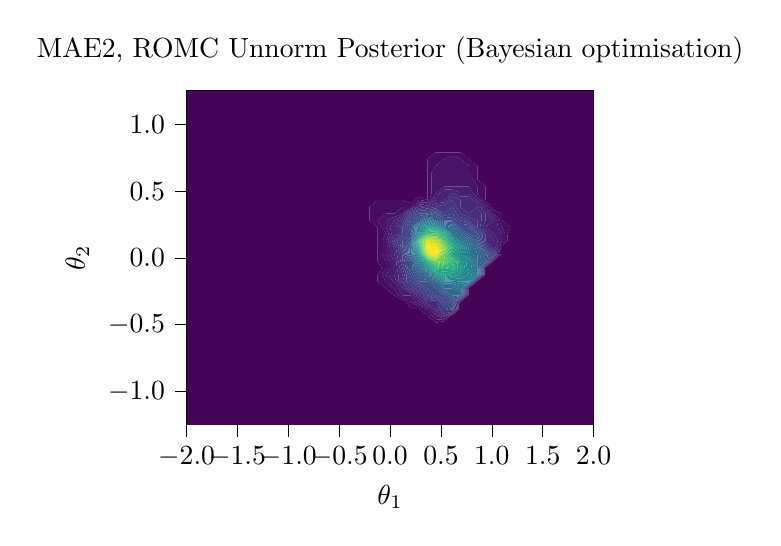
\begin{tikzpicture}

\definecolor{color0}{rgb}{0.269944,0.014625,0.341379}
\definecolor{color1}{rgb}{0.277018,0.050344,0.375715}
\definecolor{color2}{rgb}{0.280894,0.078907,0.402329}
\definecolor{color3}{rgb}{0.283091,0.110553,0.431554}
\definecolor{color4}{rgb}{0.282884,0.13592,0.453427}
\definecolor{color5}{rgb}{0.280868,0.160771,0.472899}
\definecolor{color6}{rgb}{0.276194,0.190074,0.493001}
\definecolor{color7}{rgb}{0.270595,0.214069,0.507052}
\definecolor{color8}{rgb}{0.262138,0.242286,0.520837}
\definecolor{color9}{rgb}{0.253935,0.265254,0.529983}
\definecolor{color10}{rgb}{0.243113,0.292092,0.538516}
\definecolor{color11}{rgb}{0.233603,0.313828,0.543914}
\definecolor{color12}{rgb}{0.221989,0.339161,0.548752}
\definecolor{color13}{rgb}{0.212395,0.359683,0.55171}
\definecolor{color14}{rgb}{0.203063,0.379716,0.553925}
\definecolor{color15}{rgb}{0.192357,0.403199,0.555836}
\definecolor{color16}{rgb}{0.183898,0.422383,0.556944}
\definecolor{color17}{rgb}{0.174274,0.445044,0.557792}
\definecolor{color18}{rgb}{0.166617,0.463708,0.558119}
\definecolor{color19}{rgb}{0.157729,0.485932,0.558013}
\definecolor{color20}{rgb}{0.150476,0.504369,0.55743}
\definecolor{color21}{rgb}{0.141935,0.526453,0.555991}
\definecolor{color22}{rgb}{0.135066,0.544853,0.554029}
\definecolor{color23}{rgb}{0.127568,0.566949,0.550556}
\definecolor{color24}{rgb}{0.122606,0.585371,0.546557}
\definecolor{color25}{rgb}{0.119738,0.603785,0.5414}
\definecolor{color26}{rgb}{0.120638,0.625828,0.533488}
\definecolor{color27}{rgb}{0.126326,0.644107,0.525311}
\definecolor{color28}{rgb}{0.14021,0.665859,0.513427}
\definecolor{color29}{rgb}{0.157851,0.683765,0.501686}
\definecolor{color30}{rgb}{0.185783,0.704891,0.485273}
\definecolor{color31}{rgb}{0.214,0.722114,0.469588}
\definecolor{color32}{rgb}{0.252899,0.742211,0.448284}
\definecolor{color33}{rgb}{0.288921,0.758394,0.428426}
\definecolor{color34}{rgb}{0.327796,0.77398,0.40664}
\definecolor{color35}{rgb}{0.377779,0.791781,0.377939}
\definecolor{color36}{rgb}{0.421908,0.805774,0.35191}
\definecolor{color37}{rgb}{0.477504,0.821444,0.318195}
\definecolor{color38}{rgb}{0.525776,0.833491,0.288127}
\definecolor{color39}{rgb}{0.585678,0.846661,0.249897}
\definecolor{color40}{rgb}{0.636902,0.856542,0.21662}
\definecolor{color41}{rgb}{0.699415,0.867117,0.175971}
\definecolor{color42}{rgb}{0.751884,0.874951,0.143228}
\definecolor{color43}{rgb}{0.804182,0.882046,0.114965}
\definecolor{color44}{rgb}{0.866013,0.889868,0.095953}
\definecolor{color45}{rgb}{0.916242,0.896091,0.100717}
\definecolor{color46}{rgb}{0.974417,0.90359,0.130215}

\begin{axis}[
tick align=outside,
tick pos=left,
title={MAE2, ROMC Unnorm Posterior (Bayesian optimisation)},
x grid style={white!69.0196078431373!black},
xlabel={\(\displaystyle \theta_1\)},
xmin=-2, xmax=2,
xtick style={color=black},
xtick={-2,-1.5,-1,-0.5,0,0.5,1,1.5,2},
xticklabels={
  \(\displaystyle {\ensuremath{-}2.0}\),
  \(\displaystyle {\ensuremath{-}1.5}\),
  \(\displaystyle {\ensuremath{-}1.0}\),
  \(\displaystyle {\ensuremath{-}0.5}\),
  \(\displaystyle {0.0}\),
  \(\displaystyle {0.5}\),
  \(\displaystyle {1.0}\),
  \(\displaystyle {1.5}\),
  \(\displaystyle {2.0}\)
},
y grid style={white!69.0196078431373!black},
ylabel={\(\displaystyle \theta_2\)},
ymin=-1.25, ymax=1.25,
ytick style={color=black},
ytick={-1.5,-1,-0.5,0,0.5,1,1.5},
yticklabels={
  \(\displaystyle {\ensuremath{-}1.5}\),
  \(\displaystyle {\ensuremath{-}1.0}\),
  \(\displaystyle {\ensuremath{-}0.5}\),
  \(\displaystyle {0.0}\),
  \(\displaystyle {0.5}\),
  \(\displaystyle {1.0}\),
  \(\displaystyle {1.5}\)
}
]
\addplot [draw=none, fill=color0]
table{%
x  y
-1.91836734693878 -1.25
-1.83673469387755 -1.25
-1.75510204081633 -1.25
-1.6734693877551 -1.25
-1.59183673469388 -1.25
-1.51020408163265 -1.25
-1.42857142857143 -1.25
-1.3469387755102 -1.25
-1.26530612244898 -1.25
-1.18367346938776 -1.25
-1.10204081632653 -1.25
-1.02040816326531 -1.25
-0.938775510204082 -1.25
-0.857142857142857 -1.25
-0.775510204081633 -1.25
-0.693877551020408 -1.25
-0.612244897959184 -1.25
-0.530612244897959 -1.25
-0.448979591836735 -1.25
-0.36734693877551 -1.25
-0.285714285714286 -1.25
-0.204081632653061 -1.25
-0.122448979591837 -1.25
-0.0408163265306123 -1.25
0.0408163265306123 -1.25
0.122448979591836 -1.25
0.204081632653061 -1.25
0.285714285714286 -1.25
0.36734693877551 -1.25
0.448979591836734 -1.25
0.530612244897959 -1.25
0.612244897959183 -1.25
0.693877551020408 -1.25
0.775510204081633 -1.25
0.857142857142857 -1.25
0.938775510204081 -1.25
1.02040816326531 -1.25
1.10204081632653 -1.25
1.18367346938775 -1.25
1.26530612244898 -1.25
1.3469387755102 -1.25
1.42857142857143 -1.25
1.51020408163265 -1.25
1.59183673469388 -1.25
1.6734693877551 -1.25
1.75510204081633 -1.25
1.83673469387755 -1.25
1.91836734693878 -1.25
2 -1.25
2 -1.19897959183673
2 -1.14795918367347
2 -1.0969387755102
2 -1.04591836734694
2 -0.994897959183674
2 -0.943877551020408
2 -0.892857142857143
2 -0.841836734693878
2 -0.790816326530612
2 -0.739795918367347
2 -0.688775510204082
2 -0.637755102040816
2 -0.586734693877551
2 -0.535714285714286
2 -0.48469387755102
2 -0.433673469387755
2 -0.38265306122449
2 -0.331632653061224
2 -0.280612244897959
2 -0.229591836734694
2 -0.178571428571429
2 -0.127551020408163
2 -0.0765306122448979
2 -0.0255102040816326
2 0.0255102040816326
2 0.0765306122448979
2 0.127551020408163
2 0.178571428571429
2 0.229591836734694
2 0.280612244897959
2 0.331632653061225
2 0.38265306122449
2 0.433673469387755
2 0.48469387755102
2 0.535714285714286
2 0.586734693877551
2 0.637755102040816
2 0.688775510204082
2 0.739795918367347
2 0.790816326530612
2 0.841836734693878
2 0.892857142857143
2 0.943877551020408
2 0.994897959183674
2 1.04591836734694
2 1.0969387755102
2 1.14795918367347
2 1.19897959183673
2 1.25
1.91836734693878 1.25
1.83673469387755 1.25
1.75510204081633 1.25
1.6734693877551 1.25
1.59183673469388 1.25
1.51020408163265 1.25
1.42857142857143 1.25
1.3469387755102 1.25
1.26530612244898 1.25
1.18367346938775 1.25
1.10204081632653 1.25
1.02040816326531 1.25
0.938775510204081 1.25
0.857142857142857 1.25
0.775510204081633 1.25
0.693877551020408 1.25
0.612244897959183 1.25
0.530612244897959 1.25
0.448979591836734 1.25
0.36734693877551 1.25
0.285714285714286 1.25
0.204081632653061 1.25
0.122448979591836 1.25
0.0408163265306123 1.25
-0.0408163265306123 1.25
-0.122448979591837 1.25
-0.204081632653061 1.25
-0.285714285714286 1.25
-0.36734693877551 1.25
-0.448979591836735 1.25
-0.530612244897959 1.25
-0.612244897959184 1.25
-0.693877551020408 1.25
-0.775510204081633 1.25
-0.857142857142857 1.25
-0.938775510204082 1.25
-1.02040816326531 1.25
-1.10204081632653 1.25
-1.18367346938776 1.25
-1.26530612244898 1.25
-1.3469387755102 1.25
-1.42857142857143 1.25
-1.51020408163265 1.25
-1.59183673469388 1.25
-1.6734693877551 1.25
-1.75510204081633 1.25
-1.83673469387755 1.25
-1.91836734693878 1.25
-2 1.25
-2 1.19897959183673
-2 1.14795918367347
-2 1.0969387755102
-2 1.04591836734694
-2 0.994897959183674
-2 0.943877551020408
-2 0.892857142857143
-2 0.841836734693878
-2 0.790816326530612
-2 0.739795918367347
-2 0.688775510204082
-2 0.637755102040816
-2 0.586734693877551
-2 0.535714285714286
-2 0.48469387755102
-2 0.433673469387755
-2 0.38265306122449
-2 0.331632653061225
-2 0.280612244897959
-2 0.229591836734694
-2 0.178571428571429
-2 0.127551020408163
-2 0.0765306122448979
-2 0.0255102040816326
-2 -0.0255102040816326
-2 -0.0765306122448979
-2 -0.127551020408163
-2 -0.178571428571429
-2 -0.229591836734694
-2 -0.280612244897959
-2 -0.331632653061224
-2 -0.38265306122449
-2 -0.433673469387755
-2 -0.48469387755102
-2 -0.535714285714286
-2 -0.586734693877551
-2 -0.637755102040816
-2 -0.688775510204082
-2 -0.739795918367347
-2 -0.790816326530612
-2 -0.841836734693878
-2 -0.892857142857143
-2 -0.943877551020408
-2 -0.994897959183674
-2 -1.04591836734694
-2 -1.0969387755102
-2 -1.14795918367347
-2 -1.19897959183673
-2 -1.25
-1.91836734693878 -1.25

0.36734693877551 -0.433673469387755
0.36734693877551 -0.433673469387755
0.285714285714286 -0.38265306122449
0.204081632653061 -0.38265306122449
0.163265306122449 -0.331632653061224
0.122448979591836 -0.314625850340136
0.0408163265306123 -0.280612244897959
0.0408163265306123 -0.280612244897959
-0.0408163265306123 -0.229591836734694
-0.0408163265306123 -0.229591836734694
-0.122448979591837 -0.178571428571429
-0.122448979591837 -0.127551020408163
-0.0816326530612246 -0.0765306122448979
-0.122448979591837 -0.0255102040816326
-0.122448979591837 0.0255102040816326
-0.122448979591837 0.0765306122448979
-0.122448979591837 0.127551020408163
-0.122448979591837 0.178571428571429
-0.122448979591837 0.229591836734694
-0.204081632653061 0.280612244897959
-0.204081632653061 0.331632653061225
-0.204081632653061 0.38265306122449
-0.122448979591837 0.433673469387755
-0.0408163265306123 0.433673469387755
0.0408163265306123 0.433673469387755
0.122448979591836 0.433673469387755
0.204081632653061 0.408163265306122
0.244897959183673 0.433673469387755
0.285714285714286 0.459183673469388
0.36734693877551 0.433673469387755
0.36734693877551 0.48469387755102
0.36734693877551 0.535714285714286
0.36734693877551 0.586734693877551
0.36734693877551 0.637755102040816
0.36734693877551 0.688775510204082
0.36734693877551 0.739795918367347
0.448979591836734 0.790816326530612
0.530612244897959 0.790816326530612
0.612244897959183 0.790816326530612
0.693877551020408 0.790816326530612
0.775510204081633 0.739795918367347
0.857142857142857 0.688775510204082
0.857142857142857 0.637755102040816
0.857142857142857 0.586734693877551
0.938775510204081 0.535714285714286
0.938775510204081 0.48469387755102
0.938775510204081 0.433673469387755
0.993197278911565 0.38265306122449
1.02040816326531 0.357142857142857
1.10204081632653 0.331632653061225
1.10204081632653 0.280612244897959
1.18367346938775 0.229591836734694
1.15646258503401 0.178571428571429
1.15646258503401 0.127551020408163
1.10204081632653 0.0935374149659864
1.08571428571429 0.0765306122448979
1.09297052154195 0.0255102040816326
1.02040816326531 -0.0198412698412698
1.01457725947522 -0.0255102040816326
0.938775510204081 -0.0728862973760932
0.934240362811791 -0.0765306122448979
0.934479054779806 -0.127551020408163
0.857142857142857 -0.175886143931257
0.853255587949465 -0.178571428571429
0.775510204081633 -0.227162293488824
0.770975056689342 -0.229591836734694
0.770068027210884 -0.280612244897959
0.693877551020408 -0.328231292517007
0.687074829931973 -0.331632653061224
0.685714285714286 -0.38265306122449
0.612244897959183 -0.428571428571429
0.595918367346939 -0.433673469387755
0.530612244897959 -0.474489795918367
0.448979591836734 -0.48469387755102
0.36734693877551 -0.433673469387755
};
\addplot [draw=none, fill=color1]
table{%
x  y
0.448979591836734 -0.48469387755102
0.530612244897959 -0.474489795918367
0.595918367346939 -0.433673469387755
0.612244897959183 -0.428571428571429
0.685714285714286 -0.38265306122449
0.687074829931973 -0.331632653061224
0.693877551020408 -0.328231292517007
0.770068027210884 -0.280612244897959
0.770975056689342 -0.229591836734694
0.775510204081633 -0.227162293488824
0.853255587949465 -0.178571428571429
0.857142857142857 -0.175886143931257
0.934479054779806 -0.127551020408163
0.934240362811791 -0.0765306122448979
0.938775510204081 -0.0728862973760932
1.01457725947522 -0.0255102040816326
1.02040816326531 -0.0198412698412698
1.09297052154195 0.0255102040816326
1.08571428571429 0.0765306122448979
1.10204081632653 0.0935374149659864
1.15646258503401 0.127551020408163
1.15646258503401 0.178571428571429
1.18367346938775 0.229591836734694
1.10204081632653 0.280612244897959
1.10204081632653 0.331632653061225
1.02040816326531 0.357142857142857
0.993197278911564 0.38265306122449
0.938775510204081 0.433673469387755
0.938775510204081 0.48469387755102
0.938775510204081 0.535714285714286
0.857142857142857 0.586734693877551
0.857142857142857 0.637755102040816
0.857142857142857 0.688775510204082
0.775510204081633 0.739795918367347
0.693877551020408 0.790816326530612
0.612244897959183 0.790816326530612
0.530612244897959 0.790816326530612
0.448979591836734 0.790816326530612
0.36734693877551 0.739795918367347
0.36734693877551 0.688775510204082
0.36734693877551 0.637755102040816
0.36734693877551 0.586734693877551
0.36734693877551 0.535714285714286
0.36734693877551 0.48469387755102
0.36734693877551 0.433673469387755
0.285714285714286 0.459183673469388
0.244897959183673 0.433673469387755
0.204081632653061 0.408163265306122
0.122448979591836 0.433673469387755
0.0408163265306123 0.433673469387755
-0.0408163265306123 0.433673469387755
-0.122448979591837 0.433673469387755
-0.204081632653061 0.38265306122449
-0.204081632653061 0.331632653061225
-0.204081632653061 0.280612244897959
-0.122448979591837 0.229591836734694
-0.122448979591837 0.178571428571429
-0.122448979591837 0.127551020408163
-0.122448979591837 0.0765306122448979
-0.122448979591837 0.0255102040816326
-0.122448979591837 -0.0255102040816326
-0.0816326530612246 -0.0765306122448979
-0.122448979591837 -0.127551020408163
-0.122448979591837 -0.178571428571429
-0.0408163265306123 -0.229591836734694
-0.0408163265306123 -0.229591836734694
0.0408163265306123 -0.280612244897959
0.0408163265306123 -0.280612244897959
0.122448979591836 -0.314625850340136
0.163265306122449 -0.331632653061224
0.204081632653061 -0.38265306122449
0.285714285714286 -0.38265306122449
0.36734693877551 -0.433673469387755
0.448979591836734 -0.48469387755102

0.408163265306122 -0.433673469387755
0.36734693877551 -0.38265306122449
0.285714285714286 -0.365646258503401
0.204081632653061 -0.331632653061224
0.122448979591836 -0.297619047619048
0.0816326530612244 -0.280612244897959
0.0408163265306123 -0.229591836734694
0.0408163265306123 -0.229591836734694
-0.0408163265306123 -0.178571428571429
-0.0408163265306123 -0.178571428571429
-0.0816326530612246 -0.127551020408163
-0.0408163265306123 -0.0765306122448979
-0.0408163265306123 -0.0765306122448979
-0.0408163265306123 -0.0255102040816326
-0.0408163265306123 -0.0255102040816326
-0.0816326530612246 0.0255102040816326
-0.0816326530612246 0.0765306122448979
-0.0816326530612246 0.127551020408163
-0.0408163265306123 0.178571428571429
-0.0408163265306123 0.178571428571429
-0.0408163265306123 0.178571428571429
-0.0816326530612246 0.229591836734694
-0.122448979591837 0.280612244897959
-0.0408163265306123 0.331632653061225
0.0408163265306123 0.331632653061225
0.0408163265306123 0.331632653061225
0.122448979591836 0.38265306122449
0.204081632653061 0.38265306122449
0.285714285714286 0.433673469387755
0.36734693877551 0.423469387755102
0.387755102040816 0.433673469387755
0.408163265306122 0.48469387755102
0.408163265306122 0.535714285714286
0.408163265306122 0.586734693877551
0.408163265306122 0.637755102040816
0.448979591836734 0.688775510204082
0.530612244897959 0.739795918367347
0.612244897959183 0.76530612244898
0.693877551020408 0.739795918367347
0.775510204081633 0.688775510204082
0.775510204081633 0.637755102040816
0.816326530612245 0.586734693877551
0.857142857142857 0.535714285714286
0.857142857142857 0.48469387755102
0.91156462585034 0.433673469387755
0.938775510204081 0.408163265306122
0.965986394557823 0.38265306122449
1.02040816326531 0.331632653061225
1.02040816326531 0.331632653061225
1.07482993197279 0.280612244897959
1.10204081632653 0.229591836734694
1.12925170068027 0.178571428571429
1.12925170068027 0.127551020408163
1.10204081632653 0.110544217687075
1.06938775510204 0.0765306122448979
1.08390022675737 0.0255102040816326
1.02040816326531 -0.014172335600907
1.00874635568513 -0.0255102040816326
0.938775510204081 -0.0692419825072886
0.929705215419501 -0.0765306122448979
0.930182599355531 -0.127551020408163
0.857142857142857 -0.173200859291085
0.849368318756073 -0.178571428571429
0.775510204081633 -0.224732750242954
0.766439909297052 -0.229591836734694
0.764625850340136 -0.280612244897959
0.693877551020408 -0.324829931972789
0.680272108843537 -0.331632653061224
0.677551020408163 -0.38265306122449
0.612244897959183 -0.423469387755102
0.579591836734694 -0.433673469387755
0.530612244897959 -0.464285714285714
0.448979591836734 -0.459183673469388
0.408163265306122 -0.433673469387755
};
\addplot [draw=none, fill=color2]
table{%
x  y
0.448979591836734 -0.459183673469388
0.530612244897959 -0.464285714285714
0.579591836734694 -0.433673469387755
0.612244897959183 -0.423469387755102
0.677551020408163 -0.38265306122449
0.680272108843537 -0.331632653061224
0.693877551020408 -0.324829931972789
0.764625850340136 -0.280612244897959
0.766439909297052 -0.229591836734694
0.775510204081633 -0.224732750242954
0.849368318756073 -0.178571428571429
0.857142857142857 -0.173200859291085
0.930182599355531 -0.127551020408163
0.929705215419501 -0.0765306122448979
0.938775510204081 -0.0692419825072886
1.00874635568513 -0.0255102040816326
1.02040816326531 -0.014172335600907
1.08390022675737 0.0255102040816326
1.06938775510204 0.0765306122448979
1.10204081632653 0.110544217687075
1.12925170068027 0.127551020408163
1.12925170068027 0.178571428571429
1.10204081632653 0.229591836734694
1.07482993197279 0.280612244897959
1.02040816326531 0.331632653061225
0.965986394557823 0.38265306122449
0.938775510204081 0.408163265306122
0.91156462585034 0.433673469387755
0.857142857142857 0.48469387755102
0.857142857142857 0.535714285714286
0.816326530612245 0.586734693877551
0.775510204081633 0.637755102040816
0.775510204081633 0.688775510204082
0.693877551020408 0.739795918367347
0.612244897959183 0.76530612244898
0.530612244897959 0.739795918367347
0.448979591836734 0.688775510204082
0.408163265306122 0.637755102040816
0.408163265306122 0.586734693877551
0.408163265306122 0.535714285714286
0.408163265306122 0.48469387755102
0.387755102040816 0.433673469387755
0.36734693877551 0.423469387755102
0.285714285714286 0.433673469387755
0.204081632653061 0.38265306122449
0.122448979591836 0.38265306122449
0.0408163265306123 0.331632653061225
0.0408163265306123 0.331632653061225
-0.0408163265306123 0.331632653061225
-0.122448979591837 0.280612244897959
-0.0816326530612246 0.229591836734694
-0.0408163265306123 0.178571428571429
-0.0408163265306123 0.178571428571429
-0.0816326530612246 0.127551020408163
-0.0816326530612246 0.0765306122448979
-0.0816326530612246 0.0255102040816326
-0.0408163265306123 -0.0255102040816326
-0.0408163265306123 -0.0255102040816326
-0.0408163265306123 -0.0765306122448979
-0.0408163265306123 -0.0765306122448979
-0.0816326530612246 -0.127551020408163
-0.0408163265306123 -0.178571428571429
-0.0408163265306123 -0.178571428571429
0.0408163265306123 -0.229591836734694
0.0408163265306123 -0.229591836734694
0.0816326530612244 -0.280612244897959
0.122448979591836 -0.297619047619048
0.204081632653061 -0.331632653061224
0.285714285714286 -0.365646258503401
0.36734693877551 -0.38265306122449
0.408163265306122 -0.433673469387755
0.448979591836734 -0.459183673469388

0.448979591836734 -0.433673469387755
0.387755102040816 -0.38265306122449
0.36734693877551 -0.369897959183673
0.285714285714286 -0.348639455782313
0.244897959183673 -0.331632653061224
0.204081632653061 -0.280612244897959
0.122448979591836 -0.280612244897959
0.0816326530612244 -0.229591836734694
0.0408163265306123 -0.178571428571429
0.0408163265306123 -0.178571428571429
-0.0408163265306122 -0.127551020408163
2.08166817117217e-17 -0.0765306122448979
2.08166817117217e-17 -0.0255102040816326
-0.0408163265306123 0.0255102040816326
-0.0408163265306123 0.0765306122448979
-0.0408163265306123 0.127551020408163
-0.0136054421768708 0.178571428571429
-0.0408163265306123 0.229591836734694
-0.0408163265306122 0.280612244897959
0.0408163265306123 0.306122448979592
0.122448979591836 0.331632653061225
0.204081632653061 0.374149659863946
0.231292517006803 0.38265306122449
0.285714285714286 0.416666666666667
0.36734693877551 0.413265306122449
0.408163265306122 0.433673469387755
0.448979591836734 0.48469387755102
0.530612244897959 0.535714285714286
0.612244897959183 0.535714285714286
0.693877551020408 0.535714285714286
0.775510204081633 0.535714285714286
0.816326530612245 0.48469387755102
0.857142857142857 0.459183673469388
0.884353741496598 0.433673469387755
0.938775510204081 0.38265306122449
0.993197278911564 0.331632653061225
1.02040816326531 0.306122448979592
1.04761904761905 0.280612244897959
1.06122448979592 0.229591836734694
1.10204081632653 0.178571428571429
1.10204081632653 0.127551020408163
1.0530612244898 0.0765306122448979
1.07482993197279 0.0255102040816326
1.02040816326531 -0.0085034013605442
1.00291545189504 -0.0255102040816326
0.938775510204081 -0.0655976676384839
0.925170068027211 -0.0765306122448979
0.925886143931256 -0.127551020408163
0.857142857142857 -0.170515574650913
0.845481049562682 -0.178571428571429
0.775510204081633 -0.222303206997085
0.761904761904762 -0.229591836734694
0.759183673469388 -0.280612244897959
0.693877551020408 -0.321428571428571
0.673469387755102 -0.331632653061224
0.669387755102041 -0.38265306122449
0.612244897959183 -0.418367346938775
0.563265306122449 -0.433673469387755
0.530612244897959 -0.454081632653061
0.448979591836734 -0.433673469387755
};
\addplot [draw=none, fill=color3]
table{%
x  y
0.530612244897959 -0.454081632653061
0.563265306122449 -0.433673469387755
0.612244897959183 -0.418367346938776
0.669387755102041 -0.38265306122449
0.673469387755102 -0.331632653061224
0.693877551020408 -0.321428571428571
0.759183673469388 -0.280612244897959
0.761904761904762 -0.229591836734694
0.775510204081633 -0.222303206997085
0.845481049562682 -0.178571428571429
0.857142857142857 -0.170515574650913
0.925886143931256 -0.127551020408163
0.925170068027211 -0.0765306122448979
0.938775510204081 -0.0655976676384839
1.00291545189504 -0.0255102040816326
1.02040816326531 -0.00850340136054421
1.07482993197279 0.0255102040816326
1.0530612244898 0.0765306122448979
1.10204081632653 0.127551020408163
1.10204081632653 0.178571428571429
1.06122448979592 0.229591836734694
1.04761904761905 0.280612244897959
1.02040816326531 0.306122448979592
0.993197278911564 0.331632653061225
0.938775510204081 0.38265306122449
0.884353741496598 0.433673469387755
0.857142857142857 0.459183673469388
0.816326530612245 0.48469387755102
0.775510204081633 0.535714285714286
0.693877551020408 0.535714285714286
0.612244897959183 0.535714285714286
0.530612244897959 0.535714285714286
0.448979591836734 0.48469387755102
0.408163265306122 0.433673469387755
0.36734693877551 0.413265306122449
0.285714285714286 0.416666666666667
0.231292517006803 0.38265306122449
0.204081632653061 0.374149659863946
0.122448979591836 0.331632653061225
0.0408163265306123 0.306122448979592
-0.0408163265306122 0.280612244897959
-0.0408163265306123 0.229591836734694
-0.0136054421768708 0.178571428571429
-0.0408163265306123 0.127551020408163
-0.0408163265306123 0.0765306122448979
-0.0408163265306123 0.0255102040816326
1.73472347597681e-17 -0.0255102040816326
1.73472347597681e-17 -0.0765306122448979
-0.0408163265306122 -0.127551020408163
0.0408163265306123 -0.178571428571429
0.0408163265306123 -0.178571428571429
0.0816326530612244 -0.229591836734694
0.122448979591836 -0.280612244897959
0.204081632653061 -0.280612244897959
0.244897959183673 -0.331632653061224
0.285714285714286 -0.348639455782313
0.36734693877551 -0.369897959183673
0.387755102040816 -0.38265306122449
0.448979591836734 -0.433673469387755
0.530612244897959 -0.454081632653061

0.489795918367347 -0.433673469387755
0.448979591836734 -0.416666666666667
0.408163265306122 -0.38265306122449
0.36734693877551 -0.357142857142857
0.285714285714286 -0.331632653061224
0.231292517006803 -0.280612244897959
0.204081632653061 -0.267857142857143
0.122448979591836 -0.229591836734694
0.0612244897959183 -0.178571428571429
0.0408163265306123 -0.127551020408163
0.0408163265306123 -0.0765306122448979
0.0408163265306123 -0.0255102040816326
0.0408163265306123 -0.0255102040816326
2.77555756156289e-17 0.0255102040816326
2.77555756156289e-17 0.0765306122448979
-0.0204081632653061 0.127551020408163
0.0136054421768708 0.178571428571429
2.77555756156289e-17 0.229591836734694
0.0408163265306123 0.280612244897959
0.0408163265306123 0.280612244897959
0.122448979591836 0.314625850340136
0.138775510204081 0.331632653061225
0.204081632653061 0.365646258503401
0.258503401360544 0.38265306122449
0.285714285714286 0.399659863945578
0.36734693877551 0.403061224489796
0.428571428571428 0.433673469387755
0.448979591836734 0.459183673469388
0.489795918367347 0.48469387755102
0.530612244897959 0.510204081632653
0.612244897959183 0.510204081632653
0.693877551020408 0.48469387755102
0.775510204081633 0.48469387755102
0.857142857142857 0.433673469387755
0.91156462585034 0.38265306122449
0.938775510204081 0.357142857142857
0.965986394557823 0.331632653061225
1.02040816326531 0.280612244897959
0.938775510204081 0.229591836734694
1.02040816326531 0.178571428571429
1.02040816326531 0.178571428571429
1.06122448979592 0.127551020408163
1.03673469387755 0.0765306122448979
1.06575963718821 0.0255102040816326
1.02040816326531 -0.0028344671201814
0.997084548104956 -0.0255102040816326
0.938775510204081 -0.0619533527696792
0.92063492063492 -0.0765306122448979
0.921589688506981 -0.127551020408163
0.857142857142857 -0.167830290010741
0.84159378036929 -0.178571428571429
0.775510204081633 -0.219873663751215
0.757369614512472 -0.229591836734694
0.753741496598639 -0.280612244897959
0.693877551020408 -0.318027210884354
0.666666666666667 -0.331632653061224
0.661224489795918 -0.38265306122449
0.612244897959183 -0.413265306122449
0.546938775510204 -0.433673469387755
0.530612244897959 -0.443877551020408
0.489795918367347 -0.433673469387755
};
\addplot [draw=none, fill=color4]
table{%
x  y
0.530612244897959 -0.443877551020408
0.546938775510204 -0.433673469387755
0.612244897959183 -0.413265306122449
0.661224489795918 -0.38265306122449
0.666666666666667 -0.331632653061224
0.693877551020408 -0.318027210884354
0.753741496598639 -0.280612244897959
0.757369614512472 -0.229591836734694
0.775510204081633 -0.219873663751215
0.84159378036929 -0.178571428571429
0.857142857142857 -0.167830290010741
0.921589688506981 -0.127551020408163
0.92063492063492 -0.0765306122448979
0.938775510204081 -0.0619533527696792
0.997084548104956 -0.0255102040816326
1.02040816326531 -0.0028344671201814
1.06575963718821 0.0255102040816326
1.03673469387755 0.0765306122448979
1.06122448979592 0.127551020408163
1.02040816326531 0.178571428571429
1.02040816326531 0.178571428571429
0.938775510204081 0.229591836734694
1.02040816326531 0.280612244897959
0.965986394557823 0.331632653061225
0.938775510204081 0.357142857142857
0.91156462585034 0.38265306122449
0.857142857142857 0.433673469387755
0.775510204081633 0.48469387755102
0.693877551020408 0.48469387755102
0.612244897959183 0.510204081632653
0.530612244897959 0.510204081632653
0.489795918367347 0.48469387755102
0.448979591836734 0.459183673469388
0.428571428571428 0.433673469387755
0.36734693877551 0.403061224489796
0.285714285714286 0.399659863945578
0.258503401360544 0.38265306122449
0.204081632653061 0.365646258503401
0.138775510204081 0.331632653061225
0.122448979591836 0.314625850340136
0.0408163265306123 0.280612244897959
0.0408163265306123 0.280612244897959
2.77555756156289e-17 0.229591836734694
0.0136054421768708 0.178571428571429
-0.0204081632653061 0.127551020408163
2.77555756156289e-17 0.0765306122448979
2.77555756156289e-17 0.0255102040816326
0.0408163265306123 -0.0255102040816326
0.0408163265306123 -0.0255102040816326
0.0408163265306123 -0.0765306122448979
0.0408163265306123 -0.127551020408163
0.0612244897959183 -0.178571428571429
0.122448979591836 -0.229591836734694
0.204081632653061 -0.267857142857143
0.231292517006803 -0.280612244897959
0.285714285714286 -0.331632653061224
0.36734693877551 -0.357142857142857
0.408163265306122 -0.38265306122449
0.448979591836734 -0.416666666666667
0.489795918367347 -0.433673469387755
0.530612244897959 -0.443877551020408

0.428571428571428 -0.38265306122449
0.36734693877551 -0.344387755102041
0.326530612244898 -0.331632653061224
0.285714285714286 -0.306122448979592
0.258503401360544 -0.280612244897959
0.204081632653061 -0.255102040816326
0.149659863945578 -0.229591836734694
0.122448979591836 -0.212585034013605
0.0816326530612244 -0.178571428571429
0.0816326530612244 -0.127551020408163
0.0680272108843537 -0.0765306122448979
0.0612244897959183 -0.0255102040816326
0.0408163265306123 0.0255102040816326
0.0408163265306123 0.0765306122448979
0.0408163265306123 0.0765306122448979
2.08166817117217e-17 0.127551020408163
0.0408163265306123 0.178571428571429
0.0408163265306123 0.178571428571429
0.0408163265306123 0.229591836734694
0.0816326530612244 0.280612244897959
0.122448979591836 0.297619047619048
0.155102040816326 0.331632653061225
0.204081632653061 0.357142857142857
0.285714285714286 0.38265306122449
0.36734693877551 0.392857142857143
0.448979591836734 0.433673469387755
0.530612244897959 0.433673469387755
0.612244897959183 0.48469387755102
0.693877551020408 0.459183673469388
0.775510204081633 0.459183673469388
0.816326530612245 0.433673469387755
0.857142857142857 0.408163265306122
0.884353741496598 0.38265306122449
0.938775510204081 0.331632653061225
0.938775510204081 0.280612244897959
0.91156462585034 0.229591836734694
0.938775510204081 0.204081632653061
0.979591836734694 0.178571428571429
1.02040816326531 0.127551020408163
1.02040816326531 0.0765306122448979
1.02040816326531 0.0765306122448979
1.05668934240363 0.0255102040816326
1.02040816326531 0.00283446712018141
0.991253644314869 -0.0255102040816326
0.938775510204081 -0.0583090379008746
0.91609977324263 -0.0765306122448979
0.917293233082706 -0.127551020408163
0.857142857142857 -0.165145005370569
0.837706511175899 -0.178571428571429
0.775510204081633 -0.217444120505345
0.752834467120181 -0.229591836734694
0.748299319727891 -0.280612244897959
0.693877551020408 -0.314625850340136
0.659863945578231 -0.331632653061224
0.653061224489796 -0.38265306122449
0.612244897959183 -0.408163265306122
0.530612244897959 -0.433673469387755
0.448979591836734 -0.399659863945578
0.428571428571428 -0.38265306122449
};
\addplot [draw=none, fill=color5]
table{%
x  y
0.448979591836734 -0.399659863945578
0.530612244897959 -0.433673469387755
0.612244897959183 -0.408163265306122
0.653061224489796 -0.38265306122449
0.659863945578231 -0.331632653061224
0.693877551020408 -0.314625850340136
0.748299319727891 -0.280612244897959
0.752834467120181 -0.229591836734694
0.775510204081633 -0.217444120505345
0.837706511175899 -0.178571428571429
0.857142857142857 -0.165145005370569
0.917293233082706 -0.127551020408163
0.91609977324263 -0.0765306122448979
0.938775510204081 -0.0583090379008746
0.991253644314869 -0.0255102040816326
1.02040816326531 0.00283446712018141
1.05668934240363 0.0255102040816326
1.02040816326531 0.0765306122448979
1.02040816326531 0.0765306122448979
1.02040816326531 0.127551020408163
0.979591836734694 0.178571428571429
0.938775510204081 0.204081632653061
0.91156462585034 0.229591836734694
0.938775510204081 0.280612244897959
0.938775510204081 0.331632653061225
0.884353741496598 0.38265306122449
0.857142857142857 0.408163265306122
0.816326530612245 0.433673469387755
0.775510204081633 0.459183673469388
0.693877551020408 0.459183673469388
0.612244897959183 0.48469387755102
0.530612244897959 0.433673469387755
0.448979591836734 0.433673469387755
0.36734693877551 0.392857142857143
0.285714285714286 0.38265306122449
0.204081632653061 0.357142857142857
0.155102040816326 0.331632653061225
0.122448979591836 0.297619047619048
0.0816326530612244 0.280612244897959
0.0408163265306123 0.229591836734694
0.0408163265306123 0.178571428571429
0.0408163265306123 0.178571428571429
1.73472347597681e-17 0.127551020408163
0.0408163265306123 0.0765306122448979
0.0408163265306123 0.0765306122448979
0.0408163265306123 0.0255102040816326
0.0612244897959183 -0.0255102040816326
0.0680272108843537 -0.0765306122448979
0.0816326530612244 -0.127551020408163
0.0816326530612244 -0.178571428571429
0.122448979591836 -0.212585034013605
0.149659863945578 -0.229591836734694
0.204081632653061 -0.255102040816326
0.258503401360544 -0.280612244897959
0.285714285714286 -0.306122448979592
0.326530612244898 -0.331632653061224
0.36734693877551 -0.344387755102041
0.428571428571428 -0.38265306122449
0.448979591836734 -0.399659863945578

0.448979591836734 -0.38265306122449
0.448979591836734 -0.331632653061224
0.448979591836734 -0.331632653061224
0.36734693877551 -0.331632653061224
0.285714285714286 -0.280612244897959
0.204081632653061 -0.24234693877551
0.176870748299319 -0.229591836734694
0.122448979591836 -0.195578231292517
0.10204081632653 -0.178571428571429
0.122448979591836 -0.127551020408163
0.0952380952380951 -0.0765306122448979
0.0816326530612244 -0.0255102040816326
0.0680272108843537 0.0255102040816326
0.0571428571428571 0.0765306122448979
0.0408163265306123 0.102040816326531
0.0204081632653062 0.127551020408163
0.0408163265306123 0.153061224489796
0.0680272108843537 0.178571428571429
0.0680272108843537 0.229591836734694
0.122448979591836 0.280612244897959
0.171428571428571 0.331632653061225
0.204081632653061 0.348639455782313
0.285714285714286 0.372448979591837
0.36734693877551 0.38265306122449
0.36734693877551 0.38265306122449
0.448979591836734 0.408163265306122
0.530612244897959 0.416666666666667
0.571428571428571 0.433673469387755
0.612244897959183 0.459183673469388
0.693877551020408 0.433673469387755
0.693877551020408 0.38265306122449
0.775510204081633 0.331632653061225
0.857142857142857 0.38265306122449
0.897959183673469 0.331632653061225
0.897959183673469 0.280612244897959
0.884353741496598 0.229591836734694
0.938775510204081 0.178571428571429
0.938775510204081 0.127551020408163
0.993197278911564 0.0765306122448979
1.02040816326531 0.0637755102040816
1.04761904761905 0.0255102040816326
1.02040816326531 0.00850340136054422
0.985422740524781 -0.0255102040816326
0.938775510204081 -0.0546647230320699
0.91156462585034 -0.0765306122448979
0.912996777658431 -0.127551020408163
0.857142857142857 -0.162459720730397
0.833819241982507 -0.178571428571429
0.775510204081633 -0.215014577259475
0.748299319727891 -0.229591836734694
0.742857142857143 -0.280612244897959
0.693877551020408 -0.311224489795918
0.653061224489796 -0.331632653061224
0.644897959183673 -0.38265306122449
0.612244897959183 -0.403061224489796
0.530612244897959 -0.416666666666667
0.448979591836734 -0.38265306122449
};
\addplot [draw=none, fill=color6]
table{%
x  y
0.530612244897959 -0.416666666666667
0.612244897959183 -0.403061224489796
0.644897959183673 -0.38265306122449
0.653061224489796 -0.331632653061224
0.693877551020408 -0.311224489795918
0.742857142857143 -0.280612244897959
0.748299319727891 -0.229591836734694
0.775510204081633 -0.215014577259475
0.833819241982507 -0.178571428571429
0.857142857142857 -0.162459720730397
0.912996777658431 -0.127551020408163
0.91156462585034 -0.0765306122448979
0.938775510204081 -0.0546647230320699
0.985422740524781 -0.0255102040816326
1.02040816326531 0.00850340136054421
1.04761904761905 0.0255102040816326
1.02040816326531 0.0637755102040816
0.993197278911564 0.0765306122448979
0.938775510204081 0.127551020408163
0.938775510204081 0.178571428571429
0.884353741496598 0.229591836734694
0.897959183673469 0.280612244897959
0.897959183673469 0.331632653061225
0.857142857142857 0.38265306122449
0.775510204081633 0.331632653061225
0.693877551020408 0.38265306122449
0.693877551020408 0.433673469387755
0.612244897959183 0.459183673469388
0.571428571428571 0.433673469387755
0.530612244897959 0.416666666666667
0.448979591836734 0.408163265306122
0.36734693877551 0.38265306122449
0.36734693877551 0.38265306122449
0.285714285714286 0.372448979591837
0.204081632653061 0.348639455782313
0.171428571428571 0.331632653061225
0.122448979591836 0.280612244897959
0.0680272108843537 0.229591836734694
0.0680272108843537 0.178571428571429
0.0408163265306123 0.153061224489796
0.0204081632653062 0.127551020408163
0.0408163265306123 0.102040816326531
0.0571428571428571 0.0765306122448979
0.0680272108843537 0.0255102040816326
0.0816326530612244 -0.0255102040816326
0.0952380952380951 -0.0765306122448979
0.122448979591836 -0.127551020408163
0.10204081632653 -0.178571428571429
0.122448979591836 -0.195578231292517
0.176870748299319 -0.229591836734694
0.204081632653061 -0.24234693877551
0.285714285714286 -0.280612244897959
0.36734693877551 -0.331632653061224
0.448979591836734 -0.331632653061224
0.448979591836734 -0.38265306122449
0.530612244897959 -0.416666666666667

0.489795918367347 -0.38265306122449
0.46938775510204 -0.331632653061224
0.448979591836734 -0.321428571428571
0.36734693877551 -0.314625850340136
0.312925170068027 -0.280612244897959
0.285714285714286 -0.263605442176871
0.204081632653061 -0.229591836734694
0.122448979591836 -0.178571428571429
0.142857142857143 -0.127551020408163
0.122448979591836 -0.0765306122448979
0.10204081632653 -0.0255102040816326
0.0952380952380951 0.0255102040816326
0.073469387755102 0.0765306122448979
0.0408163265306123 0.127551020408163
0.0952380952380951 0.178571428571429
0.0952380952380951 0.229591836734694
0.122448979591836 0.255102040816327
0.138775510204081 0.280612244897959
0.187755102040816 0.331632653061225
0.204081632653061 0.340136054421769
0.285714285714286 0.362244897959184
0.36734693877551 0.369897959183674
0.448979591836734 0.38265306122449
0.448979591836734 0.38265306122449
0.530612244897959 0.399659863945578
0.612244897959183 0.433673469387755
0.653061224489796 0.38265306122449
0.693877551020408 0.331632653061225
0.775510204081633 0.306122448979592
0.857142857142857 0.280612244897959
0.857142857142857 0.229591836734694
0.922448979591836 0.178571428571429
0.927113702623906 0.127551020408163
0.938775510204081 0.102040816326531
0.965986394557823 0.0765306122448979
1.02040816326531 0.0510204081632652
1.03854875283447 0.0255102040816326
1.02040816326531 0.014172335600907
0.979591836734694 -0.0255102040816326
0.938775510204081 -0.0510204081632653
0.90702947845805 -0.0765306122448979
0.908700322234156 -0.127551020408163
0.857142857142857 -0.159774436090226
0.829931972789115 -0.178571428571429
0.775510204081633 -0.212585034013605
0.743764172335601 -0.229591836734694
0.737414965986394 -0.280612244897959
0.693877551020408 -0.307823129251701
0.64625850340136 -0.331632653061224
0.636734693877551 -0.38265306122449
0.612244897959183 -0.397959183673469
0.530612244897959 -0.399659863945578
0.489795918367347 -0.38265306122449
};
\addplot [draw=none, fill=color7]
table{%
x  y
0.530612244897959 -0.399659863945578
0.612244897959183 -0.397959183673469
0.636734693877551 -0.38265306122449
0.64625850340136 -0.331632653061224
0.693877551020408 -0.307823129251701
0.737414965986394 -0.280612244897959
0.743764172335601 -0.229591836734694
0.775510204081633 -0.212585034013605
0.829931972789115 -0.178571428571429
0.857142857142857 -0.159774436090226
0.908700322234156 -0.127551020408163
0.90702947845805 -0.0765306122448979
0.938775510204081 -0.0510204081632653
0.979591836734694 -0.0255102040816326
1.02040816326531 0.014172335600907
1.03854875283447 0.0255102040816326
1.02040816326531 0.0510204081632652
0.965986394557823 0.0765306122448979
0.938775510204081 0.102040816326531
0.927113702623906 0.127551020408163
0.922448979591836 0.178571428571429
0.857142857142857 0.229591836734694
0.857142857142857 0.280612244897959
0.775510204081633 0.306122448979592
0.693877551020408 0.331632653061225
0.653061224489796 0.38265306122449
0.612244897959183 0.433673469387755
0.530612244897959 0.399659863945578
0.448979591836734 0.38265306122449
0.448979591836734 0.38265306122449
0.36734693877551 0.369897959183674
0.285714285714286 0.362244897959184
0.204081632653061 0.340136054421769
0.187755102040816 0.331632653061225
0.138775510204081 0.280612244897959
0.122448979591836 0.255102040816327
0.0952380952380951 0.229591836734694
0.0952380952380951 0.178571428571429
0.0408163265306123 0.127551020408163
0.073469387755102 0.0765306122448979
0.0952380952380951 0.0255102040816326
0.10204081632653 -0.0255102040816326
0.122448979591836 -0.0765306122448979
0.142857142857143 -0.127551020408163
0.122448979591836 -0.178571428571429
0.204081632653061 -0.229591836734694
0.285714285714286 -0.263605442176871
0.312925170068027 -0.280612244897959
0.36734693877551 -0.314625850340136
0.448979591836734 -0.321428571428571
0.46938775510204 -0.331632653061224
0.489795918367347 -0.38265306122449
0.530612244897959 -0.399659863945578

0.530612244897959 -0.38265306122449
0.489795918367347 -0.331632653061224
0.448979591836734 -0.311224489795918
0.36734693877551 -0.297619047619048
0.340136054421769 -0.280612244897959
0.285714285714286 -0.246598639455782
0.244897959183673 -0.229591836734694
0.204081632653061 -0.204081632653061
0.163265306122449 -0.178571428571429
0.163265306122449 -0.127551020408163
0.138775510204081 -0.0765306122448979
0.122448979591836 -0.0255102040816326
0.122448979591836 0.0255102040816326
0.0897959183673468 0.0765306122448979
0.0680272108843537 0.127551020408163
0.122448979591836 0.178571428571429
0.122448979591836 0.229591836734694
0.155102040816326 0.280612244897959
0.204081632653061 0.331632653061225
0.285714285714286 0.352040816326531
0.36734693877551 0.357142857142857
0.448979591836734 0.372448979591837
0.530612244897959 0.331632653061225
0.612244897959183 0.38265306122449
0.653061224489796 0.331632653061225
0.693877551020408 0.306122448979592
0.775510204081633 0.280612244897959
0.836734693877551 0.229591836734694
0.857142857142857 0.216836734693878
0.906122448979591 0.178571428571429
0.915451895043731 0.127551020408163
0.938775510204081 0.0765306122448979
1.02040816326531 0.0382653061224489
1.02947845804989 0.0255102040816326
1.02040816326531 0.0198412698412698
0.973760932944606 -0.0255102040816326
0.938775510204081 -0.0473760932944606
0.902494331065759 -0.0765306122448979
0.904403866809881 -0.127551020408163
0.857142857142857 -0.157089151450054
0.826044703595724 -0.178571428571429
0.775510204081633 -0.210155490767736
0.739229024943311 -0.229591836734694
0.731972789115646 -0.280612244897959
0.693877551020408 -0.304421768707483
0.639455782312925 -0.331632653061224
0.628571428571428 -0.38265306122449
0.612244897959183 -0.392857142857143
0.530612244897959 -0.38265306122449
};
\addplot [draw=none, fill=color8]
table{%
x  y
0.612244897959183 -0.392857142857143
0.628571428571428 -0.38265306122449
0.639455782312925 -0.331632653061224
0.693877551020408 -0.304421768707483
0.731972789115646 -0.280612244897959
0.739229024943311 -0.229591836734694
0.775510204081633 -0.210155490767736
0.826044703595724 -0.178571428571429
0.857142857142857 -0.157089151450054
0.904403866809881 -0.127551020408163
0.902494331065759 -0.0765306122448979
0.938775510204081 -0.0473760932944606
0.973760932944606 -0.0255102040816326
1.02040816326531 0.0198412698412698
1.02947845804989 0.0255102040816326
1.02040816326531 0.0382653061224489
0.938775510204081 0.0765306122448979
0.915451895043731 0.127551020408163
0.906122448979591 0.178571428571429
0.857142857142857 0.216836734693878
0.836734693877551 0.229591836734694
0.775510204081633 0.280612244897959
0.693877551020408 0.306122448979592
0.653061224489796 0.331632653061225
0.612244897959183 0.38265306122449
0.530612244897959 0.331632653061225
0.448979591836734 0.372448979591837
0.36734693877551 0.357142857142857
0.285714285714286 0.352040816326531
0.204081632653061 0.331632653061225
0.155102040816326 0.280612244897959
0.122448979591836 0.229591836734694
0.122448979591836 0.178571428571429
0.0680272108843537 0.127551020408163
0.0897959183673468 0.0765306122448979
0.122448979591836 0.0255102040816326
0.122448979591836 -0.0255102040816326
0.138775510204081 -0.0765306122448979
0.163265306122449 -0.127551020408163
0.163265306122449 -0.178571428571429
0.204081632653061 -0.204081632653061
0.244897959183673 -0.229591836734694
0.285714285714286 -0.246598639455782
0.340136054421769 -0.280612244897959
0.36734693877551 -0.297619047619048
0.448979591836734 -0.311224489795918
0.489795918367347 -0.331632653061224
0.530612244897959 -0.38265306122449
0.612244897959183 -0.392857142857143

0.571428571428571 -0.38265306122449
0.530612244897959 -0.357142857142857
0.510204081632653 -0.331632653061224
0.448979591836734 -0.301020408163265
0.36734693877551 -0.280612244897959
0.36734693877551 -0.280612244897959
0.285714285714286 -0.229591836734694
0.204081632653061 -0.178571428571429
0.183673469387755 -0.127551020408163
0.155102040816326 -0.0765306122448979
0.142857142857143 -0.0255102040816326
0.132653061224489 0.0255102040816326
0.122448979591836 0.0510204081632653
0.106122448979592 0.0765306122448979
0.0952380952380951 0.127551020408163
0.122448979591836 0.153061224489796
0.163265306122449 0.178571428571429
0.142857142857143 0.229591836734694
0.171428571428571 0.280612244897959
0.204081632653061 0.314625850340136
0.244897959183673 0.331632653061225
0.285714285714286 0.341836734693878
0.36734693877551 0.344387755102041
0.448979591836734 0.362244897959184
0.510204081632653 0.331632653061225
0.530612244897959 0.314625850340136
0.612244897959183 0.331632653061225
0.693877551020408 0.280612244897959
0.775510204081633 0.263605442176871
0.816326530612245 0.229591836734694
0.857142857142857 0.204081632653061
0.889795918367347 0.178571428571429
0.903790087463556 0.127551020408163
0.927113702623906 0.0765306122448979
0.938775510204081 0.0663265306122448
1.02040816326531 0.0255102040816326
0.967930029154519 -0.0255102040816326
0.938775510204081 -0.0437317784256559
0.897959183673469 -0.0765306122448979
0.900107411385607 -0.127551020408163
0.857142857142857 -0.154403866809882
0.822157434402332 -0.178571428571429
0.775510204081633 -0.207725947521866
0.73469387755102 -0.229591836734694
0.726530612244898 -0.280612244897959
0.693877551020408 -0.301020408163265
0.63265306122449 -0.331632653061224
0.620408163265306 -0.38265306122449
0.612244897959183 -0.387755102040816
0.571428571428571 -0.38265306122449
};
\addplot [draw=none, fill=color9]
table{%
x  y
0.612244897959183 -0.387755102040816
0.620408163265306 -0.38265306122449
0.63265306122449 -0.331632653061224
0.693877551020408 -0.301020408163265
0.726530612244898 -0.280612244897959
0.73469387755102 -0.229591836734694
0.775510204081633 -0.207725947521866
0.822157434402332 -0.178571428571429
0.857142857142857 -0.154403866809882
0.900107411385607 -0.127551020408163
0.897959183673469 -0.0765306122448979
0.938775510204081 -0.0437317784256559
0.967930029154519 -0.0255102040816326
1.02040816326531 0.0255102040816326
0.938775510204081 0.0663265306122448
0.927113702623906 0.0765306122448979
0.903790087463556 0.127551020408163
0.889795918367347 0.178571428571429
0.857142857142857 0.204081632653061
0.816326530612245 0.229591836734694
0.775510204081633 0.263605442176871
0.693877551020408 0.280612244897959
0.612244897959183 0.331632653061225
0.530612244897959 0.314625850340136
0.510204081632653 0.331632653061225
0.448979591836734 0.362244897959184
0.36734693877551 0.344387755102041
0.285714285714286 0.341836734693878
0.244897959183673 0.331632653061225
0.204081632653061 0.314625850340136
0.171428571428571 0.280612244897959
0.142857142857143 0.229591836734694
0.163265306122449 0.178571428571429
0.122448979591836 0.153061224489796
0.0952380952380951 0.127551020408163
0.106122448979592 0.0765306122448979
0.122448979591836 0.0510204081632653
0.132653061224489 0.0255102040816326
0.142857142857143 -0.0255102040816326
0.155102040816326 -0.0765306122448979
0.183673469387755 -0.127551020408163
0.204081632653061 -0.178571428571429
0.285714285714286 -0.229591836734694
0.36734693877551 -0.280612244897959
0.36734693877551 -0.280612244897959
0.448979591836734 -0.301020408163265
0.510204081632653 -0.331632653061224
0.530612244897959 -0.357142857142857
0.571428571428571 -0.38265306122449
0.612244897959183 -0.387755102040816

0.530612244897959 -0.331632653061224
0.448979591836734 -0.290816326530612
0.408163265306122 -0.280612244897959
0.36734693877551 -0.255102040816326
0.326530612244898 -0.229591836734694
0.285714285714286 -0.212585034013605
0.231292517006803 -0.178571428571429
0.204081632653061 -0.127551020408163
0.171428571428571 -0.0765306122448979
0.163265306122449 -0.0255102040816326
0.142857142857143 0.0255102040816326
0.122448979591836 0.0765306122448979
0.122448979591836 0.127551020408163
0.204081632653061 0.178571428571429
0.163265306122449 0.229591836734694
0.187755102040816 0.280612244897959
0.204081632653061 0.297619047619048
0.285714285714286 0.331632653061225
0.36734693877551 0.331632653061225
0.36734693877551 0.331632653061225
0.448979591836734 0.352040816326531
0.489795918367347 0.331632653061225
0.530612244897959 0.297619047619048
0.612244897959183 0.306122448979592
0.653061224489796 0.280612244897959
0.693877551020408 0.255102040816327
0.775510204081633 0.246598639455782
0.795918367346939 0.229591836734694
0.857142857142857 0.191326530612245
0.873469387755102 0.178571428571429
0.892128279883382 0.127551020408163
0.915451895043731 0.0765306122448979
0.938775510204081 0.0561224489795918
1 0.0255102040816326
0.962099125364431 -0.0255102040816326
0.938775510204081 -0.0400874635568513
0.893424036281179 -0.0765306122448979
0.895810955961332 -0.127551020408163
0.857142857142857 -0.15171858216971
0.818270165208941 -0.178571428571429
0.775510204081633 -0.205296404275996
0.73015873015873 -0.229591836734694
0.72108843537415 -0.280612244897959
0.693877551020408 -0.297619047619048
0.625850340136054 -0.331632653061224
0.612244897959183 -0.38265306122449
0.530612244897959 -0.331632653061224
};
\addplot [draw=none, fill=color10]
table{%
x  y
0.612244897959183 -0.38265306122449
0.625850340136054 -0.331632653061224
0.693877551020408 -0.297619047619048
0.72108843537415 -0.280612244897959
0.73015873015873 -0.229591836734694
0.775510204081633 -0.205296404275996
0.818270165208941 -0.178571428571429
0.857142857142857 -0.15171858216971
0.895810955961332 -0.127551020408163
0.893424036281179 -0.0765306122448979
0.938775510204081 -0.0400874635568513
0.962099125364431 -0.0255102040816326
1 0.0255102040816326
0.938775510204081 0.0561224489795918
0.915451895043731 0.0765306122448979
0.892128279883382 0.127551020408163
0.873469387755102 0.178571428571429
0.857142857142857 0.191326530612245
0.795918367346939 0.229591836734694
0.775510204081633 0.246598639455782
0.693877551020408 0.255102040816327
0.653061224489796 0.280612244897959
0.612244897959183 0.306122448979592
0.530612244897959 0.297619047619048
0.489795918367347 0.331632653061225
0.448979591836734 0.352040816326531
0.36734693877551 0.331632653061225
0.36734693877551 0.331632653061225
0.285714285714286 0.331632653061225
0.204081632653061 0.297619047619048
0.187755102040816 0.280612244897959
0.163265306122449 0.229591836734694
0.204081632653061 0.178571428571429
0.122448979591836 0.127551020408163
0.122448979591836 0.0765306122448979
0.142857142857143 0.0255102040816326
0.163265306122449 -0.0255102040816326
0.171428571428571 -0.0765306122448979
0.204081632653061 -0.127551020408163
0.231292517006803 -0.178571428571429
0.285714285714286 -0.212585034013605
0.326530612244898 -0.229591836734694
0.36734693877551 -0.255102040816326
0.408163265306122 -0.280612244897959
0.448979591836734 -0.290816326530612
0.530612244897959 -0.331632653061224
0.612244897959183 -0.38265306122449

0.571428571428571 -0.331632653061224
0.530612244897959 -0.306122448979592
0.448979591836734 -0.280612244897959
0.448979591836734 -0.280612244897959
0.36734693877551 -0.229591836734694
0.36734693877551 -0.229591836734694
0.285714285714286 -0.195578231292517
0.258503401360544 -0.178571428571429
0.224489795918367 -0.127551020408163
0.204081632653061 -0.102040816326531
0.187755102040816 -0.0765306122448979
0.183673469387755 -0.0255102040816326
0.153061224489796 0.0255102040816326
0.136054421768707 0.0765306122448979
0.163265306122449 0.127551020408163
0.204081632653061 0.153061224489796
0.210884353741496 0.178571428571429
0.204081632653061 0.204081632653061
0.183673469387755 0.229591836734694
0.204081632653061 0.280612244897959
0.285714285714286 0.314625850340136
0.36734693877551 0.325255102040816
0.408163265306122 0.331632653061225
0.448979591836734 0.341836734693878
0.46938775510204 0.331632653061225
0.530612244897959 0.280612244897959
0.612244897959183 0.280612244897959
0.693877551020408 0.229591836734694
0.775510204081633 0.229591836734694
0.857142857142857 0.178571428571429
0.880466472303207 0.127551020408163
0.903790087463556 0.0765306122448979
0.938775510204081 0.0459183673469387
0.979591836734694 0.0255102040816326
0.956268221574344 -0.0255102040816326
0.938775510204081 -0.0364431486880466
0.888888888888889 -0.0765306122448979
0.891514500537057 -0.127551020408163
0.857142857142857 -0.149033297529538
0.814382896015549 -0.178571428571429
0.775510204081633 -0.202866861030126
0.72562358276644 -0.229591836734694
0.715646258503401 -0.280612244897959
0.693877551020408 -0.29421768707483
0.619047619047619 -0.331632653061224
0.612244897959183 -0.357142857142857
0.571428571428571 -0.331632653061224
};
\addplot [draw=none, fill=color11]
table{%
x  y
0.612244897959183 -0.357142857142857
0.619047619047619 -0.331632653061224
0.693877551020408 -0.29421768707483
0.715646258503401 -0.280612244897959
0.72562358276644 -0.229591836734694
0.775510204081633 -0.202866861030126
0.814382896015549 -0.178571428571429
0.857142857142857 -0.149033297529538
0.891514500537057 -0.127551020408163
0.888888888888889 -0.0765306122448979
0.938775510204081 -0.0364431486880466
0.956268221574344 -0.0255102040816326
0.979591836734694 0.0255102040816326
0.938775510204081 0.0459183673469387
0.903790087463556 0.0765306122448979
0.880466472303207 0.127551020408163
0.857142857142857 0.178571428571429
0.775510204081633 0.229591836734694
0.693877551020408 0.229591836734694
0.612244897959183 0.280612244897959
0.530612244897959 0.280612244897959
0.46938775510204 0.331632653061225
0.448979591836734 0.341836734693878
0.408163265306122 0.331632653061225
0.36734693877551 0.325255102040816
0.285714285714286 0.314625850340136
0.204081632653061 0.280612244897959
0.183673469387755 0.229591836734694
0.204081632653061 0.204081632653061
0.210884353741496 0.178571428571429
0.204081632653061 0.153061224489796
0.163265306122449 0.127551020408163
0.136054421768707 0.0765306122448979
0.153061224489796 0.0255102040816326
0.183673469387755 -0.0255102040816326
0.187755102040816 -0.0765306122448979
0.204081632653061 -0.102040816326531
0.224489795918367 -0.127551020408163
0.258503401360544 -0.178571428571429
0.285714285714286 -0.195578231292517
0.36734693877551 -0.229591836734694
0.36734693877551 -0.229591836734694
0.448979591836734 -0.280612244897959
0.448979591836734 -0.280612244897959
0.530612244897959 -0.306122448979592
0.571428571428571 -0.331632653061224
0.612244897959183 -0.357142857142857

0.530612244897959 -0.280612244897959
0.448979591836734 -0.229591836734694
0.448979591836734 -0.229591836734694
0.36734693877551 -0.178571428571429
0.36734693877551 -0.178571428571429
0.285714285714286 -0.178571428571429
0.244897959183673 -0.127551020408163
0.204081632653061 -0.0765306122448979
0.204081632653061 -0.0255102040816326
0.163265306122449 0.0255102040816326
0.149659863945578 0.0765306122448979
0.204081632653061 0.127551020408163
0.217687074829932 0.178571428571429
0.204081632653061 0.229591836734694
0.244897959183673 0.280612244897959
0.285714285714286 0.297619047619048
0.36734693877551 0.318877551020408
0.448979591836734 0.331632653061225
0.510204081632653 0.280612244897959
0.530612244897959 0.27332361516035
0.612244897959183 0.270408163265306
0.677551020408163 0.229591836734694
0.693877551020408 0.216836734693878
0.775510204081633 0.178571428571429
0.857142857142857 0.153061224489796
0.868804664723032 0.127551020408163
0.892128279883382 0.0765306122448979
0.938775510204081 0.0357142857142857
0.959183673469387 0.0255102040816326
0.950437317784256 -0.0255102040816326
0.938775510204081 -0.032798833819242
0.884353741496598 -0.0765306122448979
0.887218045112782 -0.127551020408163
0.857142857142857 -0.146348012889366
0.810495626822157 -0.178571428571429
0.775510204081633 -0.200437317784257
0.72108843537415 -0.229591836734694
0.710204081632653 -0.280612244897959
0.693877551020408 -0.290816326530612
0.612244897959183 -0.331632653061224
0.530612244897959 -0.280612244897959
};
\addplot [draw=none, fill=color12]
table{%
x  y
0.612244897959183 -0.331632653061224
0.693877551020408 -0.290816326530612
0.710204081632653 -0.280612244897959
0.72108843537415 -0.229591836734694
0.775510204081633 -0.200437317784257
0.810495626822157 -0.178571428571429
0.857142857142857 -0.146348012889366
0.887218045112782 -0.127551020408163
0.884353741496598 -0.0765306122448979
0.938775510204081 -0.032798833819242
0.950437317784256 -0.0255102040816326
0.959183673469387 0.0255102040816326
0.938775510204081 0.0357142857142857
0.892128279883382 0.0765306122448979
0.868804664723032 0.127551020408163
0.857142857142857 0.153061224489796
0.775510204081633 0.178571428571429
0.693877551020408 0.216836734693878
0.677551020408163 0.229591836734694
0.612244897959183 0.270408163265306
0.530612244897959 0.27332361516035
0.510204081632653 0.280612244897959
0.448979591836734 0.331632653061225
0.36734693877551 0.318877551020408
0.285714285714286 0.297619047619048
0.244897959183673 0.280612244897959
0.204081632653061 0.229591836734694
0.217687074829932 0.178571428571429
0.204081632653061 0.127551020408163
0.149659863945578 0.0765306122448979
0.163265306122449 0.0255102040816326
0.204081632653061 -0.0255102040816326
0.204081632653061 -0.0765306122448979
0.244897959183673 -0.127551020408163
0.285714285714286 -0.178571428571429
0.36734693877551 -0.178571428571429
0.36734693877551 -0.178571428571429
0.448979591836734 -0.229591836734694
0.448979591836734 -0.229591836734694
0.530612244897959 -0.280612244897959
0.612244897959183 -0.331632653061224

0.5578231292517 -0.280612244897959
0.530612244897959 -0.267857142857143
0.46938775510204 -0.229591836734694
0.448979591836734 -0.212585034013605
0.394557823129252 -0.178571428571429
0.36734693877551 -0.165816326530612
0.285714285714286 -0.153061224489796
0.265306122448979 -0.127551020408163
0.220408163265306 -0.0765306122448979
0.213151927437641 -0.0255102040816326
0.204081632653061 -0.0127551020408163
0.173469387755102 0.0255102040816326
0.163265306122449 0.0765306122448979
0.204081632653061 0.114795918367347
0.207792207792208 0.127551020408163
0.224489795918367 0.178571428571429
0.213151927437641 0.229591836734694
0.285714285714286 0.280612244897959
0.36734693877551 0.3125
0.448979591836734 0.314625850340136
0.489795918367347 0.280612244897959
0.530612244897959 0.266034985422741
0.612244897959183 0.260204081632653
0.661224489795918 0.229591836734694
0.693877551020408 0.204081632653061
0.748299319727891 0.178571428571429
0.775510204081633 0.165816326530612
0.857142857142857 0.127551020408163
0.880466472303207 0.0765306122448979
0.938775510204081 0.0255102040816326
0.944606413994169 -0.0255102040816326
0.938775510204081 -0.0291545189504373
0.879818594104308 -0.0765306122448979
0.882921589688507 -0.127551020408163
0.857142857142857 -0.143662728249194
0.806608357628766 -0.178571428571429
0.775510204081633 -0.198007774538387
0.716553287981859 -0.229591836734694
0.704761904761905 -0.280612244897959
0.693877551020408 -0.287414965986394
0.612244897959183 -0.314625850340136
0.5578231292517 -0.280612244897959
};
\addplot [draw=none, fill=color13]
table{%
x  y
0.612244897959183 -0.314625850340136
0.693877551020408 -0.287414965986394
0.704761904761905 -0.280612244897959
0.716553287981859 -0.229591836734694
0.775510204081633 -0.198007774538387
0.806608357628766 -0.178571428571429
0.857142857142857 -0.143662728249194
0.882921589688507 -0.127551020408163
0.879818594104308 -0.0765306122448979
0.938775510204081 -0.0291545189504373
0.944606413994169 -0.0255102040816326
0.938775510204081 0.0255102040816326
0.880466472303207 0.0765306122448979
0.857142857142857 0.127551020408163
0.775510204081633 0.165816326530612
0.748299319727891 0.178571428571429
0.693877551020408 0.204081632653061
0.661224489795918 0.229591836734694
0.612244897959183 0.260204081632653
0.530612244897959 0.266034985422741
0.489795918367347 0.280612244897959
0.448979591836734 0.314625850340136
0.36734693877551 0.3125
0.285714285714286 0.280612244897959
0.213151927437642 0.229591836734694
0.224489795918367 0.178571428571429
0.207792207792208 0.127551020408163
0.204081632653061 0.114795918367347
0.163265306122449 0.0765306122448979
0.173469387755102 0.0255102040816326
0.204081632653061 -0.0127551020408163
0.213151927437642 -0.0255102040816326
0.220408163265306 -0.0765306122448979
0.265306122448979 -0.127551020408163
0.285714285714286 -0.153061224489796
0.36734693877551 -0.165816326530612
0.394557823129252 -0.178571428571429
0.448979591836734 -0.212585034013605
0.46938775510204 -0.229591836734694
0.530612244897959 -0.267857142857143
0.5578231292517 -0.280612244897959
0.612244897959183 -0.314625850340136

0.585034013605442 -0.280612244897959
0.530612244897959 -0.255102040816326
0.489795918367347 -0.229591836734694
0.448979591836734 -0.195578231292517
0.421768707482993 -0.178571428571429
0.36734693877551 -0.153061224489796
0.285714285714286 -0.127551020408163
0.236734693877551 -0.0765306122448979
0.222222222222222 -0.0255102040816326
0.204081632653061 0
0.183673469387755 0.0255102040816326
0.176870748299319 0.0765306122448979
0.204081632653061 0.102040816326531
0.211502782931354 0.127551020408163
0.231292517006803 0.178571428571429
0.222222222222222 0.229591836734694
0.285714285714286 0.274234693877551
0.302040816326531 0.280612244897959
0.36734693877551 0.306122448979592
0.448979591836734 0.297619047619048
0.46938775510204 0.280612244897959
0.530612244897959 0.258746355685131
0.612244897959183 0.25
0.644897959183673 0.229591836734694
0.693877551020408 0.191326530612245
0.72108843537415 0.178571428571429
0.775510204081633 0.153061224489796
0.829931972789115 0.127551020408163
0.857142857142857 0.102040816326531
0.868804664723032 0.0765306122448979
0.91156462585034 0.0255102040816326
0.938775510204081 -0.0255102040816326
0.875283446712018 -0.0765306122448979
0.878625134264232 -0.127551020408163
0.857142857142857 -0.140977443609022
0.802721088435374 -0.178571428571429
0.775510204081633 -0.195578231292517
0.712018140589569 -0.229591836734694
0.699319727891156 -0.280612244897959
0.693877551020408 -0.284013605442177
0.612244897959183 -0.297619047619048
0.585034013605442 -0.280612244897959
};
\addplot [draw=none, fill=color14]
table{%
x  y
0.612244897959183 -0.297619047619048
0.693877551020408 -0.284013605442177
0.699319727891156 -0.280612244897959
0.712018140589569 -0.229591836734694
0.775510204081633 -0.195578231292517
0.802721088435374 -0.178571428571429
0.857142857142857 -0.140977443609022
0.878625134264232 -0.127551020408163
0.875283446712018 -0.0765306122448979
0.938775510204081 -0.0255102040816326
0.91156462585034 0.0255102040816326
0.868804664723032 0.0765306122448979
0.857142857142857 0.102040816326531
0.829931972789115 0.127551020408163
0.775510204081633 0.153061224489796
0.72108843537415 0.178571428571429
0.693877551020408 0.191326530612245
0.644897959183673 0.229591836734694
0.612244897959183 0.25
0.530612244897959 0.258746355685131
0.46938775510204 0.280612244897959
0.448979591836734 0.297619047619048
0.36734693877551 0.306122448979592
0.302040816326531 0.280612244897959
0.285714285714286 0.274234693877551
0.222222222222222 0.229591836734694
0.231292517006803 0.178571428571429
0.211502782931354 0.127551020408163
0.204081632653061 0.102040816326531
0.176870748299319 0.0765306122448979
0.183673469387755 0.0255102040816326
0.204081632653061 0
0.222222222222222 -0.0255102040816326
0.236734693877551 -0.0765306122448979
0.285714285714286 -0.127551020408163
0.36734693877551 -0.153061224489796
0.421768707482993 -0.178571428571429
0.448979591836734 -0.195578231292517
0.489795918367347 -0.229591836734694
0.530612244897959 -0.255102040816326
0.585034013605442 -0.280612244897959
0.612244897959183 -0.297619047619048

0.510204081632653 -0.229591836734694
0.448979591836734 -0.178571428571429
0.36734693877551 -0.140306122448979
0.326530612244898 -0.127551020408163
0.285714285714286 -0.110544217687075
0.253061224489796 -0.0765306122448979
0.231292517006803 -0.0255102040816326
0.204081632653061 0.0127551020408163
0.193877551020408 0.0255102040816326
0.19047619047619 0.0765306122448979
0.204081632653061 0.0892857142857142
0.215213358070501 0.127551020408163
0.238095238095238 0.178571428571429
0.231292517006803 0.229591836734694
0.285714285714286 0.267857142857143
0.318367346938775 0.280612244897959
0.36734693877551 0.299744897959184
0.448979591836734 0.280612244897959
0.530612244897959 0.251457725947522
0.612244897959183 0.239795918367347
0.628571428571428 0.229591836734694
0.693877551020408 0.178571428571429
0.775510204081633 0.14030612244898
0.802721088435374 0.127551020408163
0.857142857142857 0.0765306122448979
0.884353741496598 0.0255102040816326
0.897959183673469 -0.0255102040816326
0.870748299319728 -0.0765306122448979
0.874328678839957 -0.127551020408163
0.857142857142857 -0.138292158968851
0.798833819241982 -0.178571428571429
0.775510204081633 -0.193148688046647
0.707482993197279 -0.229591836734694
0.693877551020408 -0.280612244897959
0.612244897959183 -0.280612244897959
0.530612244897959 -0.24234693877551
0.510204081632653 -0.229591836734694
};
\addplot [draw=none, fill=color15]
table{%
x  y
0.530612244897959 -0.24234693877551
0.612244897959183 -0.280612244897959
0.693877551020408 -0.280612244897959
0.707482993197279 -0.229591836734694
0.775510204081633 -0.193148688046647
0.798833819241982 -0.178571428571429
0.857142857142857 -0.138292158968851
0.874328678839957 -0.127551020408163
0.870748299319728 -0.0765306122448979
0.897959183673469 -0.0255102040816326
0.884353741496598 0.0255102040816326
0.857142857142857 0.0765306122448979
0.802721088435374 0.127551020408163
0.775510204081633 0.14030612244898
0.693877551020408 0.178571428571429
0.628571428571428 0.229591836734694
0.612244897959183 0.239795918367347
0.530612244897959 0.251457725947522
0.448979591836734 0.280612244897959
0.36734693877551 0.299744897959184
0.318367346938775 0.280612244897959
0.285714285714286 0.267857142857143
0.231292517006803 0.229591836734694
0.238095238095238 0.178571428571429
0.215213358070501 0.127551020408163
0.204081632653061 0.0892857142857142
0.19047619047619 0.0765306122448979
0.193877551020408 0.0255102040816326
0.204081632653061 0.0127551020408163
0.231292517006803 -0.0255102040816326
0.253061224489796 -0.0765306122448979
0.285714285714286 -0.110544217687075
0.326530612244898 -0.127551020408163
0.36734693877551 -0.140306122448979
0.448979591836734 -0.178571428571429
0.510204081632653 -0.229591836734694
0.530612244897959 -0.24234693877551

0.612244897959183 -0.229591836734694
0.530612244897959 -0.229591836734694
0.465306122448979 -0.178571428571429
0.448979591836734 -0.17219387755102
0.36734693877551 -0.127551020408163
0.285714285714286 -0.0935374149659863
0.269387755102041 -0.0765306122448979
0.240362811791383 -0.0255102040816326
0.204081632653061 0.0255102040816326
0.204081632653061 0.0765306122448979
0.218923933209647 0.127551020408163
0.244897959183673 0.178571428571429
0.240362811791383 0.229591836734694
0.285714285714286 0.261479591836735
0.33469387755102 0.280612244897959
0.36734693877551 0.293367346938776
0.421768707482993 0.280612244897959
0.448979591836734 0.274234693877551
0.530612244897959 0.244169096209913
0.612244897959183 0.229591836734694
0.666666666666667 0.178571428571429
0.693877551020408 0.16156462585034
0.775510204081633 0.127551020408163
0.836734693877551 0.0765306122448979
0.857142857142857 0.0255102040816326
0.857142857142857 -0.0255102040816326
0.866213151927437 -0.0765306122448979
0.870032223415682 -0.127551020408163
0.857142857142857 -0.135606874328679
0.794946550048591 -0.178571428571429
0.775510204081633 -0.190719144800777
0.702947845804989 -0.229591836734694
0.693877551020408 -0.263605442176871
0.612244897959183 -0.229591836734694
};
\addplot [draw=none, fill=color16]
table{%
x  y
0.693877551020408 -0.263605442176871
0.702947845804988 -0.229591836734694
0.775510204081633 -0.190719144800777
0.794946550048591 -0.178571428571429
0.857142857142857 -0.135606874328679
0.870032223415682 -0.127551020408163
0.866213151927437 -0.0765306122448979
0.857142857142857 -0.0255102040816326
0.857142857142857 0.0255102040816326
0.836734693877551 0.0765306122448979
0.775510204081633 0.127551020408163
0.693877551020408 0.16156462585034
0.666666666666667 0.178571428571429
0.612244897959183 0.229591836734694
0.530612244897959 0.244169096209913
0.448979591836734 0.274234693877551
0.421768707482993 0.280612244897959
0.36734693877551 0.293367346938776
0.33469387755102 0.280612244897959
0.285714285714286 0.261479591836735
0.240362811791383 0.229591836734694
0.244897959183673 0.178571428571429
0.218923933209647 0.127551020408163
0.204081632653061 0.0765306122448979
0.204081632653061 0.0255102040816326
0.240362811791383 -0.0255102040816326
0.269387755102041 -0.0765306122448979
0.285714285714286 -0.0935374149659863
0.36734693877551 -0.127551020408163
0.36734693877551 -0.127551020408163
0.448979591836734 -0.17219387755102
0.465306122448979 -0.178571428571429
0.530612244897959 -0.229591836734694
0.612244897959183 -0.229591836734694
0.693877551020408 -0.263605442176871

0.653061224489796 -0.229591836734694
0.612244897959183 -0.216836734693878
0.530612244897959 -0.216836734693878
0.481632653061224 -0.178571428571429
0.448979591836734 -0.165816326530612
0.379008746355685 -0.127551020408163
0.36734693877551 -0.120262390670554
0.285714285714286 -0.0765306122448979
0.249433106575964 -0.0255102040816326
0.213151927437641 0.0255102040816326
0.210361067503924 0.0765306122448979
0.222634508348794 0.127551020408163
0.251700680272109 0.178571428571429
0.249433106575964 0.229591836734694
0.285714285714286 0.255102040816327
0.351020408163265 0.280612244897959
0.36734693877551 0.286989795918367
0.394557823129251 0.280612244897959
0.448979591836734 0.267857142857143
0.530612244897959 0.236880466472303
0.571428571428571 0.229591836734694
0.612244897959183 0.204081632653061
0.639455782312925 0.178571428571429
0.693877551020408 0.144557823129252
0.73469387755102 0.127551020408163
0.775510204081633 0.110544217687075
0.816326530612245 0.0765306122448979
0.816326530612245 0.0255102040816326
0.840816326530612 -0.0255102040816326
0.857142857142857 -0.0510204081632653
0.861678004535147 -0.0765306122448979
0.865735767991407 -0.127551020408163
0.857142857142857 -0.132921589688507
0.791059280855199 -0.178571428571429
0.775510204081633 -0.188289601554908
0.698412698412698 -0.229591836734694
0.693877551020408 -0.246598639455782
0.653061224489796 -0.229591836734694
};
\addplot [draw=none, fill=color17]
table{%
x  y
0.693877551020408 -0.246598639455782
0.698412698412698 -0.229591836734694
0.775510204081633 -0.188289601554908
0.791059280855199 -0.178571428571429
0.857142857142857 -0.132921589688507
0.865735767991407 -0.127551020408163
0.861678004535147 -0.0765306122448979
0.857142857142857 -0.0510204081632653
0.840816326530612 -0.0255102040816326
0.816326530612245 0.0255102040816326
0.816326530612245 0.0765306122448979
0.775510204081633 0.110544217687075
0.73469387755102 0.127551020408163
0.693877551020408 0.144557823129252
0.639455782312925 0.178571428571429
0.612244897959183 0.204081632653061
0.571428571428571 0.229591836734694
0.530612244897959 0.236880466472303
0.448979591836734 0.267857142857143
0.394557823129251 0.280612244897959
0.36734693877551 0.286989795918367
0.351020408163265 0.280612244897959
0.285714285714286 0.255102040816327
0.249433106575964 0.229591836734694
0.251700680272109 0.178571428571429
0.222634508348794 0.127551020408163
0.210361067503924 0.0765306122448979
0.213151927437642 0.0255102040816326
0.249433106575964 -0.0255102040816326
0.285714285714286 -0.0765306122448979
0.36734693877551 -0.120262390670554
0.379008746355685 -0.127551020408163
0.448979591836734 -0.165816326530612
0.481632653061224 -0.178571428571429
0.530612244897959 -0.216836734693878
0.612244897959183 -0.216836734693878
0.653061224489796 -0.229591836734694
0.693877551020408 -0.246598639455782

0.497959183673469 -0.178571428571429
0.448979591836734 -0.159438775510204
0.39067055393586 -0.127551020408163
0.36734693877551 -0.112973760932944
0.299319727891156 -0.0765306122448979
0.285714285714286 -0.0637755102040816
0.258503401360544 -0.0255102040816326
0.222222222222222 0.0255102040816326
0.216640502354788 0.0765306122448979
0.22634508348794 0.127551020408163
0.258503401360544 0.178571428571429
0.258503401360544 0.229591836734694
0.285714285714286 0.248724489795918
0.36734693877551 0.280612244897959
0.448979591836734 0.261479591836735
0.530612244897959 0.229591836734694
0.612244897959183 0.178571428571429
0.693877551020408 0.127551020408163
0.775510204081633 0.0935374149659864
0.795918367346939 0.0765306122448979
0.775510204081633 0.0255102040816326
0.824489795918367 -0.0255102040816326
0.857142857142857 -0.0765306122448979
0.861439312567132 -0.127551020408163
0.857142857142857 -0.130236305048335
0.787172011661808 -0.178571428571429
0.775510204081633 -0.185860058309038
0.693877551020408 -0.229591836734694
0.612244897959183 -0.204081632653061
0.530612244897959 -0.204081632653061
0.497959183673469 -0.178571428571429
};
\addplot [draw=none, fill=color18]
table{%
x  y
0.530612244897959 -0.204081632653061
0.612244897959183 -0.204081632653061
0.693877551020408 -0.229591836734694
0.775510204081633 -0.185860058309038
0.787172011661808 -0.178571428571429
0.857142857142857 -0.130236305048335
0.861439312567132 -0.127551020408163
0.857142857142857 -0.0765306122448979
0.824489795918367 -0.0255102040816326
0.775510204081633 0.0255102040816326
0.795918367346939 0.0765306122448979
0.775510204081633 0.0935374149659864
0.693877551020408 0.127551020408163
0.612244897959183 0.178571428571429
0.530612244897959 0.229591836734694
0.448979591836734 0.261479591836735
0.36734693877551 0.280612244897959
0.285714285714286 0.248724489795918
0.258503401360544 0.229591836734694
0.258503401360544 0.178571428571429
0.22634508348794 0.127551020408163
0.216640502354788 0.0765306122448979
0.222222222222222 0.0255102040816326
0.258503401360544 -0.0255102040816326
0.285714285714286 -0.0637755102040816
0.299319727891156 -0.0765306122448979
0.36734693877551 -0.112973760932944
0.39067055393586 -0.127551020408163
0.448979591836734 -0.159438775510204
0.497959183673469 -0.178571428571429
0.530612244897959 -0.204081632653061

0.514285714285714 -0.178571428571429
0.448979591836734 -0.153061224489796
0.402332361516035 -0.127551020408163
0.36734693877551 -0.105685131195335
0.312925170068027 -0.0765306122448979
0.285714285714286 -0.0510204081632653
0.267573696145125 -0.0255102040816326
0.231292517006803 0.0255102040816326
0.222919937205651 0.0765306122448979
0.230055658627087 0.127551020408163
0.265306122448979 0.178571428571429
0.267573696145125 0.229591836734694
0.285714285714286 0.24234693877551
0.36734693877551 0.274234693877551
0.448979591836734 0.255102040816327
0.514285714285714 0.229591836734694
0.530612244897959 0.224953617810761
0.60482374768089 0.178571428571429
0.612244897959184 0.170068027210884
0.680272108843537 0.127551020408163
0.693877551020408 0.11734693877551
0.775510204081633 0.0765306122448979
0.755102040816326 0.0255102040816326
0.775510204081633 0.00850340136054421
0.808163265306122 -0.0255102040816326
0.829931972789115 -0.0765306122448979
0.857142857142857 -0.127551020408163
0.783284742468416 -0.178571428571429
0.775510204081633 -0.183430515063168
0.693877551020408 -0.212585034013605
0.612244897959183 -0.191326530612245
0.530612244897959 -0.191326530612245
0.514285714285714 -0.178571428571429
};
\addplot [draw=none, fill=color19]
table{%
x  y
0.530612244897959 -0.191326530612245
0.612244897959183 -0.191326530612245
0.693877551020408 -0.212585034013605
0.775510204081633 -0.183430515063168
0.783284742468416 -0.178571428571429
0.857142857142857 -0.127551020408163
0.829931972789115 -0.0765306122448979
0.808163265306122 -0.0255102040816326
0.775510204081633 0.00850340136054421
0.755102040816326 0.0255102040816326
0.775510204081633 0.0765306122448979
0.693877551020408 0.11734693877551
0.680272108843537 0.127551020408163
0.612244897959183 0.170068027210884
0.60482374768089 0.178571428571429
0.530612244897959 0.224953617810761
0.514285714285714 0.229591836734694
0.448979591836734 0.255102040816327
0.36734693877551 0.274234693877551
0.285714285714286 0.24234693877551
0.267573696145125 0.229591836734694
0.265306122448979 0.178571428571429
0.230055658627087 0.127551020408163
0.222919937205651 0.0765306122448979
0.231292517006803 0.0255102040816326
0.267573696145125 -0.0255102040816326
0.285714285714286 -0.0510204081632653
0.312925170068027 -0.0765306122448979
0.36734693877551 -0.105685131195335
0.402332361516035 -0.127551020408163
0.448979591836734 -0.153061224489796
0.514285714285714 -0.178571428571429
0.530612244897959 -0.191326530612245

0.612244897959183 -0.178571428571429
0.530612244897959 -0.178571428571429
0.448979591836734 -0.146683673469388
0.41399416909621 -0.127551020408163
0.36734693877551 -0.0983965014577258
0.326530612244898 -0.0765306122448979
0.285714285714286 -0.0382653061224489
0.276643990929705 -0.0255102040816326
0.240362811791383 0.0255102040816326
0.229199372056515 0.0765306122448979
0.233766233766234 0.127551020408163
0.272108843537415 0.178571428571429
0.276643990929705 0.229591836734694
0.285714285714286 0.235969387755102
0.36734693877551 0.267857142857143
0.448979591836734 0.248724489795918
0.497959183673469 0.229591836734694
0.530612244897959 0.220315398886827
0.597402597402597 0.178571428571429
0.612244897959183 0.16156462585034
0.666666666666667 0.127551020408163
0.693877551020408 0.107142857142857
0.755102040816326 0.0765306122448979
0.73469387755102 0.0255102040816326
0.775510204081633 -0.00850340136054421
0.791836734693877 -0.0255102040816326
0.802721088435374 -0.0765306122448979
0.829931972789115 -0.127551020408163
0.779397473275024 -0.178571428571429
0.775510204081633 -0.181000971817298
0.693877551020408 -0.195578231292517
0.612244897959183 -0.178571428571429
};
\addplot [draw=none, fill=color20]
table{%
x  y
0.693877551020408 -0.195578231292517
0.775510204081633 -0.181000971817298
0.779397473275024 -0.178571428571429
0.829931972789115 -0.127551020408163
0.802721088435374 -0.0765306122448979
0.791836734693877 -0.0255102040816326
0.775510204081633 -0.00850340136054421
0.73469387755102 0.0255102040816326
0.755102040816326 0.0765306122448979
0.693877551020408 0.107142857142857
0.666666666666667 0.127551020408163
0.612244897959183 0.16156462585034
0.597402597402597 0.178571428571429
0.530612244897959 0.220315398886827
0.497959183673469 0.229591836734694
0.448979591836734 0.248724489795918
0.36734693877551 0.267857142857143
0.285714285714286 0.235969387755102
0.276643990929705 0.229591836734694
0.272108843537415 0.178571428571429
0.233766233766234 0.127551020408163
0.229199372056515 0.0765306122448979
0.240362811791383 0.0255102040816326
0.276643990929705 -0.0255102040816326
0.285714285714286 -0.0382653061224489
0.326530612244898 -0.0765306122448979
0.36734693877551 -0.0983965014577258
0.41399416909621 -0.127551020408163
0.448979591836734 -0.146683673469388
0.530612244897959 -0.178571428571429
0.612244897959183 -0.178571428571429
0.693877551020408 -0.195578231292517

0.425655976676385 -0.127551020408163
0.36734693877551 -0.0911078717201165
0.340136054421769 -0.0765306122448979
0.285714285714286 -0.0255102040816326
0.249433106575964 0.0255102040816326
0.235478806907378 0.0765306122448979
0.23747680890538 0.127551020408163
0.27891156462585 0.178571428571429
0.285714285714286 0.229591836734694
0.36734693877551 0.261479591836735
0.448979591836734 0.24234693877551
0.481632653061224 0.229591836734694
0.530612244897959 0.215677179962894
0.589981447124304 0.178571428571429
0.612244897959183 0.153061224489796
0.653061224489796 0.127551020408163
0.693877551020408 0.0969387755102041
0.73469387755102 0.0765306122448979
0.714285714285714 0.0255102040816326
0.775510204081633 -0.0255102040816326
0.775510204081633 -0.0765306122448979
0.802721088435374 -0.127551020408163
0.775510204081633 -0.178571428571429
0.693877551020408 -0.178571428571429
0.612244897959183 -0.168367346938776
0.530612244897959 -0.171282798833819
0.448979591836734 -0.140306122448979
0.425655976676385 -0.127551020408163
};
\addplot [draw=none, fill=color21]
table{%
x  y
0.448979591836734 -0.140306122448979
0.530612244897959 -0.171282798833819
0.612244897959183 -0.168367346938776
0.693877551020408 -0.178571428571429
0.775510204081633 -0.178571428571429
0.802721088435374 -0.127551020408163
0.775510204081633 -0.0765306122448979
0.775510204081633 -0.0255102040816326
0.714285714285714 0.0255102040816326
0.73469387755102 0.0765306122448979
0.693877551020408 0.0969387755102041
0.653061224489796 0.127551020408163
0.612244897959183 0.153061224489796
0.589981447124304 0.178571428571429
0.530612244897959 0.215677179962894
0.481632653061224 0.229591836734694
0.448979591836734 0.24234693877551
0.36734693877551 0.261479591836735
0.285714285714286 0.229591836734694
0.27891156462585 0.178571428571429
0.23747680890538 0.127551020408163
0.235478806907378 0.0765306122448979
0.249433106575964 0.0255102040816326
0.285714285714286 -0.0255102040816326
0.340136054421769 -0.0765306122448979
0.36734693877551 -0.0911078717201165
0.425655976676385 -0.127551020408163
0.448979591836734 -0.140306122448979

0.437317784256559 -0.127551020408163
0.36734693877551 -0.0838192419825072
0.353741496598639 -0.0765306122448979
0.294784580498866 -0.0255102040816326
0.285714285714286 -0.0127551020408163
0.258503401360544 0.0255102040816326
0.241758241758242 0.0765306122448979
0.241187384044527 0.127551020408163
0.285714285714286 0.178571428571429
0.302040816326531 0.229591836734694
0.36734693877551 0.255102040816327
0.448979591836734 0.235969387755102
0.465306122448979 0.229591836734694
0.530612244897959 0.211038961038961
0.582560296846011 0.178571428571429
0.612244897959183 0.144557823129252
0.639455782312925 0.127551020408163
0.693877551020408 0.086734693877551
0.714285714285714 0.0765306122448979
0.693877551020408 0.0255102040816326
0.748299319727891 -0.0255102040816326
0.755102040816326 -0.0765306122448979
0.775510204081633 -0.127551020408163
0.693877551020408 -0.153061224489796
0.612244897959183 -0.158163265306122
0.530612244897959 -0.16399416909621
0.448979591836734 -0.133928571428571
0.437317784256559 -0.127551020408163
};
\addplot [draw=none, fill=color22]
table{%
x  y
0.448979591836734 -0.133928571428571
0.530612244897959 -0.16399416909621
0.612244897959183 -0.158163265306122
0.693877551020408 -0.153061224489796
0.775510204081633 -0.127551020408163
0.755102040816326 -0.0765306122448979
0.748299319727891 -0.0255102040816326
0.693877551020408 0.0255102040816326
0.714285714285714 0.0765306122448979
0.693877551020408 0.086734693877551
0.639455782312925 0.127551020408163
0.612244897959183 0.144557823129252
0.582560296846011 0.178571428571429
0.530612244897959 0.211038961038961
0.465306122448979 0.229591836734694
0.448979591836734 0.235969387755102
0.36734693877551 0.255102040816327
0.302040816326531 0.229591836734694
0.285714285714286 0.178571428571429
0.241187384044527 0.127551020408163
0.241758241758242 0.0765306122448979
0.258503401360544 0.0255102040816326
0.285714285714286 -0.0127551020408163
0.294784580498866 -0.0255102040816326
0.353741496598639 -0.0765306122448979
0.36734693877551 -0.0838192419825072
0.437317784256559 -0.127551020408163
0.448979591836734 -0.133928571428571

0.448979591836734 -0.127551020408163
0.448979591836734 -0.127551020408163
0.36734693877551 -0.0765306122448979
0.36734693877551 -0.0765306122448978
0.303854875283447 -0.0255102040816326
0.285714285714286 0
0.267573696145125 0.0255102040816326
0.248037676609105 0.0765306122448979
0.244897959183673 0.127551020408163
0.285714285714286 0.174319727891156
0.293135435992579 0.178571428571429
0.318367346938775 0.229591836734694
0.36734693877551 0.248724489795918
0.448979591836734 0.229591836734694
0.448979591836734 0.229591836734694
0.530612244897959 0.206400742115028
0.575139146567718 0.178571428571429
0.612244897959183 0.136054421768708
0.625850340136054 0.127551020408163
0.693877551020408 0.0765306122448979
0.677551020408163 0.0255102040816326
0.693877551020408 0
0.72108843537415 -0.0255102040816326
0.73469387755102 -0.0765306122448979
0.693877551020408 -0.127551020408163
0.612244897959183 -0.147959183673469
0.530612244897959 -0.156705539358601
0.448979591836734 -0.127551020408163
};
\addplot [draw=none, fill=color23]
table{%
x  y
0.530612244897959 -0.156705539358601
0.612244897959183 -0.147959183673469
0.693877551020408 -0.127551020408163
0.73469387755102 -0.0765306122448979
0.72108843537415 -0.0255102040816326
0.693877551020408 0
0.677551020408163 0.0255102040816326
0.693877551020408 0.0765306122448979
0.625850340136054 0.127551020408163
0.612244897959184 0.136054421768708
0.575139146567718 0.178571428571429
0.530612244897959 0.206400742115028
0.448979591836734 0.229591836734694
0.448979591836734 0.229591836734694
0.36734693877551 0.248724489795918
0.318367346938775 0.229591836734694
0.293135435992579 0.178571428571429
0.285714285714286 0.174319727891157
0.244897959183673 0.127551020408163
0.248037676609105 0.0765306122448979
0.267573696145125 0.0255102040816326
0.285714285714286 0
0.303854875283447 -0.0255102040816326
0.36734693877551 -0.0765306122448978
0.36734693877551 -0.0765306122448979
0.448979591836734 -0.127551020408163
0.448979591836734 -0.127551020408163
0.530612244897959 -0.156705539358601

0.469387755102041 -0.127551020408163
0.448979591836734 -0.121173469387755
0.377551020408163 -0.0765306122448979
0.36734693877551 -0.0692419825072885
0.312925170068027 -0.0255102040816326
0.285714285714286 0.0127551020408163
0.276643990929705 0.0255102040816326
0.254317111459968 0.0765306122448979
0.24860853432282 0.127551020408163
0.285714285714286 0.170068027210884
0.300556586270872 0.178571428571429
0.33469387755102 0.229591836734694
0.36734693877551 0.24234693877551
0.421768707482993 0.229591836734694
0.448979591836734 0.224953617810761
0.530612244897959 0.201762523191095
0.567717996289425 0.178571428571429
0.612244897959183 0.127551020408163
0.680272108843537 0.0765306122448979
0.661224489795918 0.0255102040816326
0.693877551020408 -0.0255102040816326
0.714285714285714 -0.0765306122448979
0.693877551020408 -0.102040816326531
0.653061224489796 -0.127551020408163
0.612244897959183 -0.137755102040816
0.530612244897959 -0.149416909620991
0.469387755102041 -0.127551020408163
};
\addplot [draw=none, fill=color24]
table{%
x  y
0.530612244897959 -0.149416909620991
0.612244897959183 -0.137755102040816
0.653061224489796 -0.127551020408163
0.693877551020408 -0.102040816326531
0.714285714285714 -0.0765306122448979
0.693877551020408 -0.0255102040816326
0.661224489795918 0.0255102040816326
0.680272108843537 0.0765306122448979
0.612244897959183 0.127551020408163
0.567717996289425 0.178571428571429
0.530612244897959 0.201762523191095
0.448979591836734 0.224953617810761
0.421768707482993 0.229591836734694
0.36734693877551 0.24234693877551
0.33469387755102 0.229591836734694
0.300556586270872 0.178571428571429
0.285714285714286 0.170068027210884
0.24860853432282 0.127551020408163
0.254317111459968 0.0765306122448979
0.276643990929705 0.0255102040816326
0.285714285714286 0.0127551020408163
0.312925170068027 -0.0255102040816326
0.36734693877551 -0.0692419825072885
0.377551020408163 -0.0765306122448979
0.448979591836734 -0.121173469387755
0.469387755102041 -0.127551020408163
0.530612244897959 -0.149416909620991

0.489795918367347 -0.127551020408163
0.448979591836734 -0.114795918367347
0.387755102040816 -0.0765306122448979
0.36734693877551 -0.0619533527696792
0.321995464852608 -0.0255102040816326
0.285714285714286 0.0255102040816326
0.260596546310832 0.0765306122448979
0.252319109461966 0.127551020408163
0.285714285714286 0.165816326530612
0.307977736549165 0.178571428571429
0.351020408163265 0.229591836734694
0.36734693877551 0.235969387755102
0.394557823129251 0.229591836734694
0.448979591836734 0.220315398886827
0.530612244897959 0.197124304267161
0.560296846011131 0.178571428571429
0.604081632653061 0.127551020408163
0.612244897959183 0.11734693877551
0.666666666666667 0.0765306122448979
0.644897959183673 0.0255102040816326
0.683673469387755 -0.0255102040816326
0.693877551020408 -0.0765306122448979
0.612244897959183 -0.127551020408163
0.530612244897959 -0.142128279883382
0.489795918367347 -0.127551020408163
};
\addplot [draw=none, fill=color25]
table{%
x  y
0.530612244897959 -0.142128279883382
0.612244897959183 -0.127551020408163
0.693877551020408 -0.0765306122448979
0.683673469387755 -0.0255102040816326
0.644897959183673 0.0255102040816326
0.666666666666667 0.0765306122448979
0.612244897959183 0.11734693877551
0.604081632653061 0.127551020408163
0.560296846011131 0.178571428571429
0.530612244897959 0.197124304267161
0.448979591836734 0.220315398886827
0.394557823129251 0.229591836734694
0.36734693877551 0.235969387755102
0.351020408163265 0.229591836734694
0.307977736549165 0.178571428571429
0.285714285714286 0.165816326530612
0.252319109461966 0.127551020408163
0.260596546310832 0.0765306122448979
0.285714285714286 0.0255102040816326
0.321995464852608 -0.0255102040816326
0.36734693877551 -0.0619533527696792
0.387755102040816 -0.0765306122448979
0.448979591836734 -0.114795918367347
0.489795918367347 -0.127551020408163
0.530612244897959 -0.142128279883382

0.510204081632653 -0.127551020408163
0.448979591836734 -0.108418367346939
0.397959183673469 -0.0765306122448979
0.36734693877551 -0.0546647230320699
0.331065759637188 -0.0255102040816326
0.290249433106576 0.0255102040816326
0.285714285714286 0.0382653061224489
0.266875981161695 0.0765306122448979
0.256029684601113 0.127551020408163
0.285714285714286 0.16156462585034
0.315398886827458 0.178571428571429
0.36734693877551 0.229591836734694
0.448979591836734 0.215677179962894
0.530612244897959 0.192486085343228
0.552875695732838 0.178571428571429
0.595918367346939 0.127551020408163
0.612244897959183 0.107142857142857
0.653061224489796 0.0765306122448979
0.628571428571428 0.0255102040816326
0.673469387755102 -0.0255102040816326
0.677551020408163 -0.0765306122448979
0.612244897959183 -0.11734693877551
0.571428571428571 -0.127551020408163
0.530612244897959 -0.134839650145772
0.510204081632653 -0.127551020408163
};
\addplot [draw=none, fill=color26]
table{%
x  y
0.530612244897959 -0.134839650145772
0.571428571428571 -0.127551020408163
0.612244897959183 -0.11734693877551
0.677551020408163 -0.0765306122448979
0.673469387755102 -0.0255102040816326
0.628571428571428 0.0255102040816326
0.653061224489796 0.0765306122448979
0.612244897959183 0.107142857142857
0.595918367346939 0.127551020408163
0.552875695732838 0.178571428571429
0.530612244897959 0.192486085343228
0.448979591836734 0.215677179962894
0.36734693877551 0.229591836734694
0.315398886827458 0.178571428571429
0.285714285714286 0.16156462585034
0.256029684601113 0.127551020408163
0.266875981161695 0.0765306122448979
0.285714285714286 0.0382653061224489
0.290249433106576 0.0255102040816326
0.331065759637188 -0.0255102040816326
0.36734693877551 -0.0546647230320699
0.397959183673469 -0.0765306122448979
0.448979591836734 -0.108418367346939
0.510204081632653 -0.127551020408163
0.530612244897959 -0.134839650145772

0.408163265306122 -0.0765306122448979
0.36734693877551 -0.0473760932944606
0.340136054421769 -0.0255102040816326
0.294784580498866 0.0255102040816326
0.285714285714286 0.0510204081632653
0.273155416012559 0.0765306122448979
0.25974025974026 0.127551020408163
0.285714285714286 0.157312925170068
0.322820037105751 0.178571428571429
0.36734693877551 0.222303206997085
0.448979591836734 0.211038961038961
0.530612244897959 0.187847866419295
0.545454545454545 0.178571428571429
0.587755102040816 0.127551020408163
0.612244897959183 0.0969387755102041
0.639455782312925 0.0765306122448979
0.612244897959183 0.0255102040816326
0.663265306122449 -0.0255102040816326
0.661224489795918 -0.0765306122448979
0.612244897959183 -0.107142857142857
0.530612244897959 -0.127551020408163
0.448979591836734 -0.10204081632653
0.408163265306122 -0.0765306122448979
};
\addplot [draw=none, fill=color27]
table{%
x  y
0.448979591836734 -0.10204081632653
0.530612244897959 -0.127551020408163
0.612244897959183 -0.107142857142857
0.661224489795918 -0.0765306122448979
0.663265306122449 -0.0255102040816326
0.612244897959183 0.0255102040816326
0.639455782312925 0.0765306122448979
0.612244897959183 0.0969387755102041
0.587755102040816 0.127551020408163
0.545454545454545 0.178571428571429
0.530612244897959 0.187847866419295
0.448979591836734 0.211038961038961
0.36734693877551 0.222303206997085
0.322820037105751 0.178571428571429
0.285714285714286 0.157312925170068
0.25974025974026 0.127551020408163
0.273155416012559 0.0765306122448979
0.285714285714286 0.0510204081632653
0.294784580498866 0.0255102040816326
0.340136054421769 -0.0255102040816326
0.36734693877551 -0.0473760932944606
0.408163265306122 -0.0765306122448979
0.448979591836734 -0.10204081632653

0.418367346938775 -0.0765306122448979
0.36734693877551 -0.0400874635568512
0.349206349206349 -0.0255102040816326
0.299319727891156 0.0255102040816326
0.285714285714286 0.0637755102040816
0.279434850863422 0.0765306122448979
0.263450834879406 0.127551020408163
0.285714285714286 0.153061224489796
0.330241187384045 0.178571428571429
0.36734693877551 0.215014577259475
0.448979591836734 0.206400742115028
0.530612244897959 0.183209647495362
0.538033395176252 0.178571428571429
0.579591836734694 0.127551020408163
0.612244897959183 0.086734693877551
0.625850340136054 0.0765306122448979
0.612244897959183 0.0510204081632653
0.604081632653061 0.0255102040816326
0.612244897959183 0.0153061224489796
0.653061224489796 -0.0255102040816326
0.644897959183673 -0.0765306122448979
0.612244897959183 -0.096938775510204
0.530612244897959 -0.102040816326531
0.448979591836734 -0.0956632653061223
0.418367346938775 -0.0765306122448979
};
\addplot [draw=none, fill=color28]
table{%
x  y
0.448979591836734 -0.0956632653061223
0.530612244897959 -0.102040816326531
0.612244897959183 -0.096938775510204
0.644897959183673 -0.0765306122448979
0.653061224489796 -0.0255102040816326
0.612244897959183 0.0153061224489796
0.604081632653061 0.0255102040816326
0.612244897959183 0.0510204081632653
0.625850340136054 0.0765306122448979
0.612244897959183 0.086734693877551
0.579591836734694 0.127551020408163
0.538033395176252 0.178571428571429
0.530612244897959 0.183209647495362
0.448979591836734 0.206400742115028
0.36734693877551 0.215014577259475
0.330241187384045 0.178571428571429
0.285714285714286 0.153061224489796
0.263450834879406 0.127551020408163
0.279434850863422 0.0765306122448979
0.285714285714286 0.0637755102040816
0.299319727891156 0.0255102040816326
0.349206349206349 -0.0255102040816326
0.36734693877551 -0.0400874635568512
0.418367346938775 -0.0765306122448979
0.448979591836734 -0.0956632653061223

0.428571428571428 -0.0765306122448979
0.36734693877551 -0.0327988338192419
0.35827664399093 -0.0255102040816326
0.303854875283447 0.0255102040816326
0.285714285714286 0.0765306122448979
0.267161410018553 0.127551020408163
0.285714285714286 0.148809523809524
0.337662337662338 0.178571428571429
0.36734693877551 0.207725947521866
0.448979591836734 0.201762523191095
0.530612244897959 0.178571428571429
0.571428571428571 0.127551020408163
0.612244897959183 0.0765306122448979
0.595918367346939 0.0255102040816326
0.612244897959183 0.00510204081632652
0.642857142857143 -0.0255102040816326
0.628571428571428 -0.0765306122448979
0.612244897959183 -0.0867346938775509
0.530612244897959 -0.0765306122448979
0.448979591836734 -0.0892857142857142
0.428571428571428 -0.0765306122448979
};
\addplot [draw=none, fill=color29]
table{%
x  y
0.448979591836734 -0.0892857142857142
0.530612244897959 -0.0765306122448979
0.612244897959183 -0.0867346938775509
0.628571428571428 -0.0765306122448979
0.642857142857143 -0.0255102040816326
0.612244897959183 0.00510204081632652
0.595918367346939 0.0255102040816326
0.612244897959183 0.0765306122448979
0.571428571428571 0.127551020408163
0.530612244897959 0.178571428571429
0.448979591836734 0.201762523191095
0.36734693877551 0.207725947521866
0.337662337662338 0.178571428571429
0.285714285714286 0.148809523809524
0.267161410018553 0.127551020408163
0.285714285714286 0.0765306122448979
0.303854875283447 0.0255102040816326
0.35827664399093 -0.0255102040816326
0.36734693877551 -0.0327988338192419
0.428571428571428 -0.0765306122448979
0.448979591836734 -0.0892857142857142

0.438775510204081 -0.0765306122448979
0.36734693877551 -0.0255102040816326
0.36734693877551 -0.0255102040816326
0.308390022675737 0.0255102040816326
0.290249433106576 0.0765306122448979
0.285714285714286 0.086734693877551
0.270871985157699 0.127551020408163
0.285714285714286 0.144557823129252
0.345083487940631 0.178571428571429
0.36734693877551 0.200437317784257
0.448979591836734 0.197124304267161
0.514285714285714 0.178571428571429
0.530612244897959 0.168367346938776
0.563265306122449 0.127551020408163
0.604081632653061 0.0765306122448979
0.587755102040816 0.0255102040816326
0.612244897959183 -0.00510204081632652
0.63265306122449 -0.0255102040816326
0.612244897959183 -0.0765306122448979
0.530612244897959 -0.0692419825072886
0.489795918367347 -0.0765306122448979
0.448979591836734 -0.082908163265306
0.438775510204081 -0.0765306122448979
};
\addplot [draw=none, fill=color30]
table{%
x  y
0.448979591836734 -0.082908163265306
0.489795918367347 -0.0765306122448979
0.530612244897959 -0.0692419825072886
0.612244897959183 -0.0765306122448979
0.63265306122449 -0.0255102040816326
0.612244897959183 -0.00510204081632652
0.587755102040816 0.0255102040816326
0.604081632653061 0.0765306122448979
0.563265306122449 0.127551020408163
0.530612244897959 0.168367346938776
0.514285714285714 0.178571428571429
0.448979591836734 0.197124304267161
0.36734693877551 0.200437317784257
0.345083487940631 0.178571428571429
0.285714285714286 0.144557823129252
0.270871985157699 0.127551020408163
0.285714285714286 0.086734693877551
0.290249433106576 0.0765306122448979
0.308390022675737 0.0255102040816326
0.36734693877551 -0.0255102040816326
0.36734693877551 -0.0255102040816326
0.438775510204081 -0.0765306122448979
0.448979591836734 -0.082908163265306

0.377551020408163 -0.0255102040816326
0.36734693877551 -0.021585557299843
0.312925170068027 0.0255102040816326
0.294784580498866 0.0765306122448979
0.285714285714286 0.0969387755102041
0.274582560296846 0.127551020408163
0.285714285714286 0.14030612244898
0.352504638218924 0.178571428571429
0.36734693877551 0.193148688046647
0.448979591836734 0.192486085343228
0.497959183673469 0.178571428571429
0.530612244897959 0.158163265306123
0.555102040816326 0.127551020408163
0.595918367346939 0.0765306122448979
0.579591836734694 0.0255102040816326
0.612244897959183 -0.0153061224489796
0.622448979591837 -0.0255102040816326
0.612244897959183 -0.0510204081632653
0.530612244897959 -0.0619533527696792
0.448979591836734 -0.0765306122448978
0.377551020408163 -0.0255102040816326
};
\addplot [draw=none, fill=color31]
table{%
x  y
0.448979591836734 -0.0765306122448978
0.530612244897959 -0.0619533527696792
0.612244897959183 -0.0510204081632653
0.622448979591837 -0.0255102040816326
0.612244897959183 -0.0153061224489796
0.579591836734694 0.0255102040816326
0.595918367346939 0.0765306122448979
0.555102040816326 0.127551020408163
0.530612244897959 0.158163265306123
0.497959183673469 0.178571428571429
0.448979591836734 0.192486085343228
0.36734693877551 0.193148688046647
0.352504638218924 0.178571428571429
0.285714285714286 0.14030612244898
0.274582560296846 0.127551020408163
0.285714285714286 0.0969387755102041
0.294784580498866 0.0765306122448979
0.312925170068027 0.0255102040816326
0.36734693877551 -0.021585557299843
0.377551020408163 -0.0255102040816326
0.448979591836734 -0.0765306122448978

0.387755102040816 -0.0255102040816326
0.36734693877551 -0.0176609105180533
0.317460317460317 0.0255102040816326
0.299319727891156 0.0765306122448979
0.285714285714286 0.107142857142857
0.278293135435992 0.127551020408163
0.285714285714286 0.136054421768708
0.359925788497217 0.178571428571429
0.36734693877551 0.185860058309038
0.448979591836734 0.187847866419295
0.481632653061224 0.178571428571429
0.530612244897959 0.147959183673469
0.546938775510204 0.127551020408163
0.587755102040816 0.0765306122448979
0.571428571428571 0.0255102040816326
0.612244897959183 -0.0255102040816326
0.530612244897959 -0.0546647230320699
0.448979591836734 -0.0692419825072885
0.387755102040816 -0.0255102040816326
};
\addplot [draw=none, fill=color32]
table{%
x  y
0.448979591836734 -0.0692419825072885
0.530612244897959 -0.0546647230320699
0.612244897959183 -0.0255102040816326
0.571428571428571 0.0255102040816326
0.587755102040816 0.0765306122448979
0.546938775510204 0.127551020408163
0.530612244897959 0.147959183673469
0.481632653061224 0.178571428571429
0.448979591836734 0.187847866419295
0.36734693877551 0.185860058309038
0.359925788497217 0.178571428571429
0.285714285714286 0.136054421768708
0.278293135435992 0.127551020408163
0.285714285714286 0.107142857142857
0.299319727891156 0.0765306122448979
0.317460317460317 0.0255102040816326
0.36734693877551 -0.0176609105180533
0.387755102040816 -0.0255102040816326
0.448979591836734 -0.0692419825072885

0.397959183673469 -0.0255102040816326
0.36734693877551 -0.0137362637362637
0.321995464852608 0.0255102040816326
0.303854875283447 0.0765306122448979
0.285714285714286 0.11734693877551
0.282003710575139 0.127551020408163
0.285714285714286 0.131802721088435
0.36734693877551 0.178571428571429
0.367346938775511 0.178571428571429
0.448979591836734 0.183209647495362
0.465306122448979 0.178571428571429
0.530612244897959 0.137755102040816
0.538775510204081 0.127551020408163
0.579591836734694 0.0765306122448979
0.563265306122449 0.0255102040816326
0.591836734693877 -0.0255102040816326
0.530612244897959 -0.0473760932944606
0.448979591836734 -0.0619533527696792
0.397959183673469 -0.0255102040816326
};
\addplot [draw=none, fill=color33]
table{%
x  y
0.448979591836734 -0.0619533527696792
0.530612244897959 -0.0473760932944606
0.591836734693877 -0.0255102040816326
0.563265306122449 0.0255102040816326
0.579591836734694 0.0765306122448979
0.538775510204081 0.127551020408163
0.530612244897959 0.137755102040816
0.465306122448979 0.178571428571429
0.448979591836734 0.183209647495362
0.367346938775511 0.178571428571429
0.36734693877551 0.178571428571429
0.285714285714286 0.131802721088435
0.282003710575139 0.127551020408163
0.285714285714286 0.11734693877551
0.303854875283447 0.0765306122448979
0.321995464852608 0.0255102040816326
0.36734693877551 -0.0137362637362637
0.397959183673469 -0.0255102040816326
0.448979591836734 -0.0619533527696792

0.408163265306122 -0.0255102040816326
0.36734693877551 -0.00981161695447407
0.326530612244898 0.0255102040816326
0.308390022675737 0.0765306122448979
0.285714285714286 0.127551020408163
0.36734693877551 0.173933209647495
0.448979591836734 0.178571428571429
0.530612244897959 0.127551020408163
0.571428571428571 0.0765306122448979
0.555102040816326 0.0255102040816326
0.571428571428571 -0.0255102040816326
0.530612244897959 -0.0400874635568513
0.448979591836734 -0.0546647230320699
0.408163265306122 -0.0255102040816326
};
\addplot [draw=none, fill=color34]
table{%
x  y
0.448979591836734 -0.0546647230320699
0.530612244897959 -0.0400874635568513
0.571428571428571 -0.0255102040816326
0.555102040816326 0.0255102040816326
0.571428571428571 0.0765306122448979
0.530612244897959 0.127551020408163
0.448979591836734 0.178571428571429
0.36734693877551 0.173933209647495
0.285714285714286 0.127551020408163
0.308390022675737 0.0765306122448979
0.326530612244898 0.0255102040816326
0.36734693877551 -0.00981161695447407
0.408163265306122 -0.0255102040816326
0.448979591836734 -0.0546647230320699

0.418367346938775 -0.0255102040816326
0.36734693877551 -0.00588697017268443
0.331065759637188 0.0255102040816326
0.312925170068027 0.0765306122448979
0.293877551020408 0.127551020408163
0.36734693877551 0.169294990723562
0.448979591836734 0.17219387755102
0.520408163265306 0.127551020408163
0.530612244897959 0.11734693877551
0.563265306122449 0.0765306122448979
0.546938775510204 0.0255102040816326
0.551020408163265 -0.0255102040816326
0.530612244897959 -0.032798833819242
0.448979591836734 -0.0473760932944605
0.418367346938775 -0.0255102040816326
};
\addplot [draw=none, fill=color35]
table{%
x  y
0.448979591836734 -0.0473760932944606
0.530612244897959 -0.032798833819242
0.551020408163265 -0.0255102040816326
0.546938775510204 0.0255102040816326
0.563265306122449 0.0765306122448979
0.530612244897959 0.11734693877551
0.520408163265306 0.127551020408163
0.448979591836734 0.17219387755102
0.36734693877551 0.169294990723562
0.293877551020408 0.127551020408163
0.312925170068027 0.0765306122448979
0.331065759637188 0.0255102040816326
0.36734693877551 -0.00588697017268443
0.418367346938775 -0.0255102040816326
0.448979591836734 -0.0473760932944606

0.428571428571428 -0.0255102040816326
0.36734693877551 -0.0019623233908948
0.335600907029478 0.0255102040816326
0.317460317460317 0.0765306122448979
0.302040816326531 0.127551020408163
0.36734693877551 0.164656771799629
0.448979591836734 0.165816326530612
0.510204081632653 0.127551020408163
0.530612244897959 0.107142857142857
0.555102040816326 0.0765306122448979
0.538775510204081 0.0255102040816326
0.530612244897959 -0.0255102040816326
0.448979591836734 -0.0400874635568512
0.428571428571428 -0.0255102040816326
};
\addplot [draw=none, fill=color36]
table{%
x  y
0.448979591836734 -0.0400874635568512
0.530612244897959 -0.0255102040816326
0.538775510204081 0.0255102040816326
0.555102040816326 0.0765306122448979
0.530612244897959 0.107142857142857
0.510204081632653 0.127551020408163
0.448979591836734 0.165816326530612
0.36734693877551 0.164656771799629
0.302040816326531 0.127551020408163
0.317460317460317 0.0765306122448979
0.335600907029478 0.0255102040816326
0.36734693877551 -0.0019623233908948
0.428571428571428 -0.0255102040816326
0.448979591836734 -0.0400874635568512

0.438775510204081 -0.0255102040816326
0.36734693877551 0.00196232339089484
0.340136054421769 0.0255102040816326
0.321995464852608 0.0765306122448979
0.310204081632653 0.127551020408163
0.36734693877551 0.160018552875696
0.448979591836734 0.159438775510204
0.5 0.127551020408163
0.530612244897959 0.0969387755102041
0.546938775510204 0.0765306122448979
0.530612244897959 0.0255102040816326
0.489795918367346 -0.0255102040816326
0.448979591836734 -0.0327988338192419
0.438775510204081 -0.0255102040816326
};
\addplot [draw=none, fill=color37]
table{%
x  y
0.448979591836734 -0.0327988338192419
0.489795918367346 -0.0255102040816326
0.530612244897959 0.0255102040816326
0.546938775510204 0.0765306122448979
0.530612244897959 0.0969387755102041
0.5 0.127551020408163
0.448979591836734 0.159438775510204
0.36734693877551 0.160018552875696
0.310204081632653 0.127551020408163
0.321995464852608 0.0765306122448979
0.340136054421769 0.0255102040816326
0.36734693877551 0.00196232339089484
0.438775510204081 -0.0255102040816326
0.448979591836734 -0.0327988338192419

0.344671201814059 0.0255102040816326
0.326530612244898 0.0765306122448979
0.318367346938775 0.127551020408163
0.36734693877551 0.155380333951763
0.448979591836734 0.153061224489796
0.489795918367347 0.127551020408163
0.530612244897959 0.086734693877551
0.538775510204081 0.0765306122448979
0.530612244897959 0.0510204081632653
0.522448979591836 0.0255102040816326
0.448979591836734 -0.0255102040816326
0.36734693877551 0.00588697017268448
0.344671201814059 0.0255102040816326
};
\addplot [draw=none, fill=color38]
table{%
x  y
0.36734693877551 0.00588697017268447
0.448979591836734 -0.0255102040816326
0.522448979591836 0.0255102040816326
0.530612244897959 0.0510204081632653
0.538775510204081 0.0765306122448979
0.530612244897959 0.086734693877551
0.489795918367347 0.127551020408163
0.448979591836734 0.153061224489796
0.36734693877551 0.155380333951763
0.318367346938775 0.127551020408163
0.326530612244898 0.0765306122448979
0.344671201814059 0.0255102040816326
0.36734693877551 0.00588697017268447

0.349206349206349 0.0255102040816326
0.331065759637188 0.0765306122448979
0.326530612244898 0.127551020408163
0.36734693877551 0.150742115027829
0.448979591836734 0.146683673469388
0.479591836734693 0.127551020408163
0.530612244897959 0.0765306122448979
0.514285714285714 0.0255102040816326
0.448979591836734 -0.0198412698412698
0.36734693877551 0.00981161695447411
0.349206349206349 0.0255102040816326
};
\addplot [draw=none, fill=color39]
table{%
x  y
0.36734693877551 0.00981161695447411
0.448979591836734 -0.0198412698412698
0.514285714285714 0.0255102040816326
0.530612244897959 0.0765306122448979
0.479591836734693 0.127551020408163
0.448979591836734 0.146683673469388
0.36734693877551 0.150742115027829
0.326530612244898 0.127551020408163
0.331065759637188 0.0765306122448979
0.349206349206349 0.0255102040816326
0.36734693877551 0.00981161695447411

0.353741496598639 0.0255102040816326
0.335600907029478 0.0765306122448979
0.33469387755102 0.127551020408163
0.36734693877551 0.146103896103896
0.448979591836734 0.14030612244898
0.46938775510204 0.127551020408163
0.520408163265306 0.0765306122448979
0.506122448979591 0.0255102040816326
0.448979591836734 -0.014172335600907
0.36734693877551 0.0137362637362637
0.353741496598639 0.0255102040816326
};
\addplot [draw=none, fill=color40]
table{%
x  y
0.36734693877551 0.0137362637362637
0.448979591836734 -0.014172335600907
0.506122448979591 0.0255102040816326
0.520408163265306 0.0765306122448979
0.46938775510204 0.127551020408163
0.448979591836734 0.14030612244898
0.36734693877551 0.146103896103896
0.33469387755102 0.127551020408163
0.335600907029478 0.0765306122448979
0.353741496598639 0.0255102040816326
0.36734693877551 0.0137362637362637

0.35827664399093 0.0255102040816326
0.340136054421769 0.0765306122448979
0.342857142857143 0.127551020408163
0.36734693877551 0.141465677179963
0.448979591836734 0.133928571428571
0.459183673469387 0.127551020408163
0.510204081632653 0.0765306122448979
0.497959183673469 0.0255102040816326
0.448979591836734 -0.00850340136054417
0.36734693877551 0.0176609105180534
0.35827664399093 0.0255102040816326
};
\addplot [draw=none, fill=color41]
table{%
x  y
0.36734693877551 0.0176609105180534
0.448979591836734 -0.00850340136054417
0.497959183673469 0.0255102040816326
0.510204081632653 0.0765306122448979
0.459183673469387 0.127551020408163
0.448979591836734 0.133928571428571
0.36734693877551 0.141465677179963
0.342857142857143 0.127551020408163
0.340136054421769 0.0765306122448979
0.35827664399093 0.0255102040816326
0.36734693877551 0.0176609105180534

0.36281179138322 0.0255102040816326
0.344671201814059 0.0765306122448979
0.351020408163265 0.127551020408163
0.36734693877551 0.13682745825603
0.448979591836734 0.127551020408163
0.448979591836734 0.127551020408163
0.5 0.0765306122448979
0.489795918367347 0.0255102040816326
0.448979591836734 -0.00283446712018136
0.36734693877551 0.021585557299843
0.36281179138322 0.0255102040816326
};
\addplot [draw=none, fill=color42]
table{%
x  y
0.36734693877551 0.021585557299843
0.448979591836734 -0.00283446712018137
0.489795918367347 0.0255102040816326
0.5 0.0765306122448979
0.448979591836734 0.127551020408163
0.448979591836734 0.127551020408163
0.36734693877551 0.13682745825603
0.351020408163265 0.127551020408163
0.344671201814059 0.0765306122448979
0.36281179138322 0.0255102040816326
0.36734693877551 0.021585557299843

0.36734693877551 0.0255102040816326
0.36734693877551 0.0255102040816327
0.349206349206349 0.0765306122448979
0.359183673469388 0.127551020408163
0.36734693877551 0.132189239332097
0.408163265306122 0.127551020408163
0.448979591836734 0.11734693877551
0.489795918367347 0.0765306122448979
0.481632653061224 0.0255102040816326
0.448979591836734 0.00283446712018144
0.36734693877551 0.0255102040816326
};
\addplot [draw=none, fill=color43]
table{%
x  y
0.448979591836734 0.00283446712018144
0.481632653061224 0.0255102040816326
0.489795918367347 0.0765306122448979
0.448979591836734 0.11734693877551
0.408163265306122 0.127551020408163
0.36734693877551 0.132189239332097
0.359183673469388 0.127551020408163
0.349206349206349 0.0765306122448979
0.36734693877551 0.0255102040816327
0.36734693877551 0.0255102040816326
0.448979591836734 0.00283446712018144

0.387755102040816 0.0255102040816326
0.36734693877551 0.038265306122449
0.353741496598639 0.0765306122448979
0.36734693877551 0.127551020408163
0.448979591836734 0.107142857142857
0.479591836734693 0.0765306122448979
0.473469387755102 0.0255102040816326
0.448979591836734 0.00850340136054425
0.387755102040816 0.0255102040816326
};
\addplot [draw=none, fill=color44]
table{%
x  y
0.448979591836734 0.00850340136054425
0.473469387755102 0.0255102040816326
0.479591836734693 0.0765306122448979
0.448979591836734 0.107142857142857
0.36734693877551 0.127551020408163
0.353741496598639 0.0765306122448979
0.36734693877551 0.038265306122449
0.387755102040816 0.0255102040816326
0.448979591836734 0.00850340136054425

0.408163265306122 0.0255102040816326
0.36734693877551 0.0510204081632653
0.35827664399093 0.0765306122448979
0.36734693877551 0.110544217687075
0.448979591836734 0.096938775510204
0.46938775510204 0.0765306122448979
0.465306122448979 0.0255102040816326
0.448979591836734 0.0141723356009071
0.408163265306122 0.0255102040816326
};
\addplot [draw=none, fill=color45]
table{%
x  y
0.448979591836734 0.0141723356009071
0.465306122448979 0.0255102040816326
0.46938775510204 0.0765306122448979
0.448979591836734 0.096938775510204
0.36734693877551 0.110544217687075
0.35827664399093 0.0765306122448979
0.36734693877551 0.0510204081632653
0.408163265306122 0.0255102040816326
0.448979591836734 0.0141723356009071

0.428571428571428 0.0255102040816326
0.36734693877551 0.0637755102040817
0.36281179138322 0.0765306122448979
0.36734693877551 0.0935374149659862
0.448979591836734 0.0867346938775509
0.459183673469387 0.0765306122448979
0.457142857142857 0.0255102040816326
0.448979591836734 0.0198412698412699
0.428571428571428 0.0255102040816326
};
\addplot [draw=none, fill=color46]
table{%
x  y
0.448979591836734 0.0198412698412699
0.457142857142857 0.0255102040816326
0.459183673469387 0.0765306122448979
0.448979591836734 0.0867346938775509
0.36734693877551 0.0935374149659862
0.36281179138322 0.0765306122448979
0.36734693877551 0.0637755102040817
0.428571428571428 0.0255102040816326
0.448979591836734 0.0198412698412699
};
\end{axis}

\end{tikzpicture}

    }
    \resizebox{.32\columnwidth}{!}{%
      % This file was created with tikzplotlib v0.9.12.
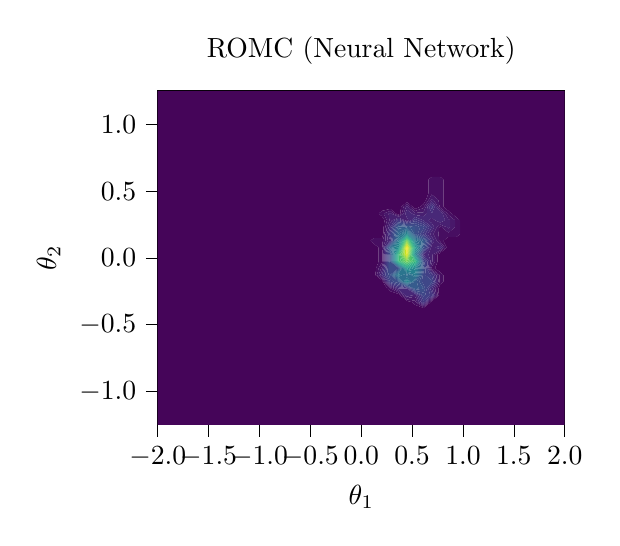
\begin{tikzpicture}

\definecolor{color0}{rgb}{0.271305,0.019942,0.347269}
\definecolor{color1}{rgb}{0.277941,0.056324,0.381191}
\definecolor{color2}{rgb}{0.282327,0.094955,0.417331}
\definecolor{color3}{rgb}{0.283187,0.125848,0.44496}
\definecolor{color4}{rgb}{0.281412,0.155834,0.469201}
\definecolor{color5}{rgb}{0.276194,0.190074,0.493001}
\definecolor{color6}{rgb}{0.269308,0.218818,0.509577}
\definecolor{color7}{rgb}{0.258965,0.251537,0.524736}
\definecolor{color8}{rgb}{0.248629,0.278775,0.534556}
\definecolor{color9}{rgb}{0.237441,0.305202,0.541921}
\definecolor{color10}{rgb}{0.223925,0.334994,0.548053}
\definecolor{color11}{rgb}{0.212395,0.359683,0.55171}
\definecolor{color12}{rgb}{0.19943,0.387607,0.554642}
\definecolor{color13}{rgb}{0.188923,0.41091,0.556326}
\definecolor{color14}{rgb}{0.179019,0.433756,0.55743}
\definecolor{color15}{rgb}{0.168126,0.459988,0.558082}
\definecolor{color16}{rgb}{0.159194,0.482237,0.558073}
\definecolor{color17}{rgb}{0.150476,0.504369,0.55743}
\definecolor{color18}{rgb}{0.140536,0.530132,0.555659}
\definecolor{color19}{rgb}{0.132444,0.552216,0.553018}
\definecolor{color20}{rgb}{0.124395,0.578002,0.548287}
\definecolor{color21}{rgb}{0.120092,0.600104,0.54253}
\definecolor{color22}{rgb}{0.120638,0.625828,0.533488}
\definecolor{color23}{rgb}{0.128087,0.647749,0.523491}
\definecolor{color24}{rgb}{0.143303,0.669459,0.511215}
\definecolor{color25}{rgb}{0.170948,0.694384,0.493803}
\definecolor{color26}{rgb}{0.202219,0.715272,0.476084}
\definecolor{color27}{rgb}{0.24607,0.73891,0.452024}
\definecolor{color28}{rgb}{0.288921,0.758394,0.428426}
\definecolor{color29}{rgb}{0.335885,0.777018,0.402049}
\definecolor{color30}{rgb}{0.395174,0.797475,0.367757}
\definecolor{color31}{rgb}{0.449368,0.813768,0.335384}
\definecolor{color32}{rgb}{0.515992,0.831158,0.294279}
\definecolor{color33}{rgb}{0.575563,0.844566,0.256415}
\definecolor{color34}{rgb}{0.636902,0.856542,0.21662}
\definecolor{color35}{rgb}{0.709898,0.868751,0.169257}
\definecolor{color36}{rgb}{0.772852,0.877868,0.131109}
\definecolor{color37}{rgb}{0.845561,0.887322,0.099702}
\definecolor{color38}{rgb}{0.906311,0.894855,0.098125}
\definecolor{color39}{rgb}{0.964894,0.902323,0.123941}

\begin{axis}[
tick align=outside,
tick pos=left,
title={ROMC (Neural Network)},
x grid style={white!69.0196078431373!black},
xlabel={\(\displaystyle \theta_1\)},
xmin=-2, xmax=2,
xtick style={color=black},
xtick={-2,-1.5,-1,-0.5,0,0.5,1,1.5,2},
xticklabels={
  \(\displaystyle {\ensuremath{-}2.0}\),
  \(\displaystyle {\ensuremath{-}1.5}\),
  \(\displaystyle {\ensuremath{-}1.0}\),
  \(\displaystyle {\ensuremath{-}0.5}\),
  \(\displaystyle {0.0}\),
  \(\displaystyle {0.5}\),
  \(\displaystyle {1.0}\),
  \(\displaystyle {1.5}\),
  \(\displaystyle {2.0}\)
},
y grid style={white!69.0196078431373!black},
ylabel={\(\displaystyle \theta_2\)},
ymin=-1.25, ymax=1.25,
ytick style={color=black},
ytick={-1.5,-1,-0.5,0,0.5,1,1.5},
yticklabels={
  \(\displaystyle {\ensuremath{-}1.5}\),
  \(\displaystyle {\ensuremath{-}1.0}\),
  \(\displaystyle {\ensuremath{-}0.5}\),
  \(\displaystyle {0.0}\),
  \(\displaystyle {0.5}\),
  \(\displaystyle {1.0}\),
  \(\displaystyle {1.5}\)
}
]
\addplot [draw=none, fill=color0]
table{%
x  y
-1.91836734693878 -1.25
-1.83673469387755 -1.25
-1.75510204081633 -1.25
-1.6734693877551 -1.25
-1.59183673469388 -1.25
-1.51020408163265 -1.25
-1.42857142857143 -1.25
-1.3469387755102 -1.25
-1.26530612244898 -1.25
-1.18367346938776 -1.25
-1.10204081632653 -1.25
-1.02040816326531 -1.25
-0.938775510204082 -1.25
-0.857142857142857 -1.25
-0.775510204081633 -1.25
-0.693877551020408 -1.25
-0.612244897959184 -1.25
-0.530612244897959 -1.25
-0.448979591836735 -1.25
-0.36734693877551 -1.25
-0.285714285714286 -1.25
-0.204081632653061 -1.25
-0.122448979591837 -1.25
-0.0408163265306123 -1.25
0.0408163265306123 -1.25
0.122448979591836 -1.25
0.204081632653061 -1.25
0.285714285714286 -1.25
0.36734693877551 -1.25
0.448979591836734 -1.25
0.530612244897959 -1.25
0.612244897959183 -1.25
0.693877551020408 -1.25
0.775510204081633 -1.25
0.857142857142857 -1.25
0.938775510204081 -1.25
1.02040816326531 -1.25
1.10204081632653 -1.25
1.18367346938775 -1.25
1.26530612244898 -1.25
1.3469387755102 -1.25
1.42857142857143 -1.25
1.51020408163265 -1.25
1.59183673469388 -1.25
1.6734693877551 -1.25
1.75510204081633 -1.25
1.83673469387755 -1.25
1.91836734693878 -1.25
2 -1.25
2 -1.19897959183673
2 -1.14795918367347
2 -1.0969387755102
2 -1.04591836734694
2 -0.994897959183674
2 -0.943877551020408
2 -0.892857142857143
2 -0.841836734693878
2 -0.790816326530612
2 -0.739795918367347
2 -0.688775510204082
2 -0.637755102040816
2 -0.586734693877551
2 -0.535714285714286
2 -0.48469387755102
2 -0.433673469387755
2 -0.38265306122449
2 -0.331632653061224
2 -0.280612244897959
2 -0.229591836734694
2 -0.178571428571429
2 -0.127551020408163
2 -0.0765306122448979
2 -0.0255102040816326
2 0.0255102040816326
2 0.0765306122448979
2 0.127551020408163
2 0.178571428571429
2 0.229591836734694
2 0.280612244897959
2 0.331632653061225
2 0.38265306122449
2 0.433673469387755
2 0.48469387755102
2 0.535714285714286
2 0.586734693877551
2 0.637755102040816
2 0.688775510204082
2 0.739795918367347
2 0.790816326530612
2 0.841836734693878
2 0.892857142857143
2 0.943877551020408
2 0.994897959183674
2 1.04591836734694
2 1.0969387755102
2 1.14795918367347
2 1.19897959183673
2 1.25
1.91836734693878 1.25
1.83673469387755 1.25
1.75510204081633 1.25
1.6734693877551 1.25
1.59183673469388 1.25
1.51020408163265 1.25
1.42857142857143 1.25
1.3469387755102 1.25
1.26530612244898 1.25
1.18367346938775 1.25
1.10204081632653 1.25
1.02040816326531 1.25
0.938775510204081 1.25
0.857142857142857 1.25
0.775510204081633 1.25
0.693877551020408 1.25
0.612244897959183 1.25
0.530612244897959 1.25
0.448979591836734 1.25
0.36734693877551 1.25
0.285714285714286 1.25
0.204081632653061 1.25
0.122448979591836 1.25
0.0408163265306123 1.25
-0.0408163265306123 1.25
-0.122448979591837 1.25
-0.204081632653061 1.25
-0.285714285714286 1.25
-0.36734693877551 1.25
-0.448979591836735 1.25
-0.530612244897959 1.25
-0.612244897959184 1.25
-0.693877551020408 1.25
-0.775510204081633 1.25
-0.857142857142857 1.25
-0.938775510204082 1.25
-1.02040816326531 1.25
-1.10204081632653 1.25
-1.18367346938776 1.25
-1.26530612244898 1.25
-1.3469387755102 1.25
-1.42857142857143 1.25
-1.51020408163265 1.25
-1.59183673469388 1.25
-1.6734693877551 1.25
-1.75510204081633 1.25
-1.83673469387755 1.25
-1.91836734693878 1.25
-2 1.25
-2 1.19897959183673
-2 1.14795918367347
-2 1.0969387755102
-2 1.04591836734694
-2 0.994897959183674
-2 0.943877551020408
-2 0.892857142857143
-2 0.841836734693878
-2 0.790816326530612
-2 0.739795918367347
-2 0.688775510204082
-2 0.637755102040816
-2 0.586734693877551
-2 0.535714285714286
-2 0.48469387755102
-2 0.433673469387755
-2 0.38265306122449
-2 0.331632653061225
-2 0.280612244897959
-2 0.229591836734694
-2 0.178571428571429
-2 0.127551020408163
-2 0.0765306122448979
-2 0.0255102040816326
-2 -0.0255102040816326
-2 -0.0765306122448979
-2 -0.127551020408163
-2 -0.178571428571429
-2 -0.229591836734694
-2 -0.280612244897959
-2 -0.331632653061224
-2 -0.38265306122449
-2 -0.433673469387755
-2 -0.48469387755102
-2 -0.535714285714286
-2 -0.586734693877551
-2 -0.637755102040816
-2 -0.688775510204082
-2 -0.739795918367347
-2 -0.790816326530612
-2 -0.841836734693878
-2 -0.892857142857143
-2 -0.943877551020408
-2 -0.994897959183674
-2 -1.04591836734694
-2 -1.0969387755102
-2 -1.14795918367347
-2 -1.19897959183673
-2 -1.25
-1.91836734693878 -1.25

0.497959183673469 -0.331632653061224
0.448979591836734 -0.321428571428571
0.383673469387755 -0.280612244897959
0.36734693877551 -0.270408163265306
0.285714285714286 -0.25
0.253061224489796 -0.229591836734694
0.213877551020408 -0.178571428571429
0.204081632653061 -0.168367346938776
0.138775510204081 -0.127551020408163
0.146938775510204 -0.0765306122448979
0.171428571428571 -0.0255102040816326
0.171428571428571 0.0255102040816326
0.171428571428571 0.0765306122448979
0.122448979591836 0.107142857142857
0.0897959183673468 0.127551020408163
0.122448979591836 0.147959183673469
0.204081632653061 0.147959183673469
0.216326530612245 0.178571428571429
0.220408163265306 0.229591836734694
0.228571428571428 0.280612244897959
0.204081632653061 0.311224489795918
0.171428571428571 0.331632653061225
0.204081632653061 0.352040816326531
0.285714285714286 0.36734693877551
0.342857142857143 0.331632653061225
0.36734693877551 0.323979591836735
0.383673469387755 0.331632653061225
0.391836734693877 0.38265306122449
0.448979591836734 0.418367346938776
0.506122448979592 0.38265306122449
0.530612244897959 0.36734693877551
0.579591836734694 0.38265306122449
0.612244897959183 0.403061224489796
0.636734693877551 0.433673469387755
0.661224489795918 0.48469387755102
0.661224489795918 0.535714285714286
0.661224489795918 0.586734693877551
0.693877551020408 0.607142857142857
0.775510204081633 0.607142857142857
0.808163265306122 0.586734693877551
0.808163265306122 0.535714285714286
0.808163265306122 0.48469387755102
0.808163265306122 0.433673469387755
0.808163265306122 0.38265306122449
0.857142857142857 0.352040816326531
0.889795918367347 0.331632653061225
0.938775510204081 0.301020408163265
0.971428571428571 0.280612244897959
0.971428571428571 0.229591836734694
0.971428571428571 0.178571428571429
0.938775510204081 0.158163265306123
0.857142857142857 0.158163265306123
0.808163265306122 0.127551020408163
0.840816326530612 0.0765306122448979
0.775510204081633 0.0357142857142857
0.751020408163265 0.0255102040816326
0.751020408163265 -0.0255102040816326
0.726530612244898 -0.0765306122448979
0.775510204081633 -0.107142857142857
0.808163265306122 -0.127551020408163
0.808163265306122 -0.178571428571429
0.775510204081633 -0.198979591836735
0.759183673469388 -0.229591836734694
0.763265306122449 -0.280612244897959
0.693877551020408 -0.323979591836735
0.681632653061224 -0.331632653061224
0.612244897959183 -0.375
0.530612244897959 -0.352040816326531
0.497959183673469 -0.331632653061224
};
\addplot [draw=none, fill=color1]
table{%
x  y
0.530612244897959 -0.352040816326531
0.612244897959183 -0.375
0.681632653061224 -0.331632653061224
0.693877551020408 -0.323979591836735
0.763265306122449 -0.280612244897959
0.759183673469388 -0.229591836734694
0.775510204081633 -0.198979591836735
0.808163265306122 -0.178571428571429
0.808163265306122 -0.127551020408163
0.775510204081633 -0.107142857142857
0.726530612244898 -0.0765306122448979
0.751020408163265 -0.0255102040816326
0.751020408163265 0.0255102040816326
0.775510204081633 0.0357142857142857
0.840816326530612 0.0765306122448979
0.808163265306122 0.127551020408163
0.857142857142857 0.158163265306123
0.938775510204081 0.158163265306123
0.971428571428571 0.178571428571429
0.971428571428571 0.229591836734694
0.971428571428571 0.280612244897959
0.938775510204081 0.301020408163265
0.889795918367347 0.331632653061225
0.857142857142857 0.352040816326531
0.808163265306122 0.38265306122449
0.808163265306122 0.433673469387755
0.808163265306122 0.48469387755102
0.808163265306122 0.535714285714286
0.808163265306122 0.586734693877551
0.775510204081633 0.607142857142857
0.693877551020408 0.607142857142857
0.661224489795918 0.586734693877551
0.661224489795918 0.535714285714286
0.661224489795918 0.48469387755102
0.636734693877551 0.433673469387755
0.612244897959183 0.403061224489796
0.579591836734694 0.38265306122449
0.530612244897959 0.36734693877551
0.506122448979591 0.38265306122449
0.448979591836734 0.418367346938776
0.391836734693877 0.38265306122449
0.383673469387755 0.331632653061225
0.36734693877551 0.323979591836735
0.342857142857143 0.331632653061225
0.285714285714286 0.36734693877551
0.204081632653061 0.352040816326531
0.171428571428571 0.331632653061225
0.204081632653061 0.311224489795918
0.228571428571428 0.280612244897959
0.220408163265306 0.229591836734694
0.216326530612245 0.178571428571429
0.204081632653061 0.147959183673469
0.122448979591836 0.147959183673469
0.0897959183673468 0.127551020408163
0.122448979591836 0.107142857142857
0.171428571428571 0.0765306122448979
0.171428571428571 0.0255102040816326
0.171428571428571 -0.0255102040816326
0.146938775510204 -0.0765306122448979
0.138775510204081 -0.127551020408163
0.204081632653061 -0.168367346938776
0.213877551020408 -0.178571428571429
0.253061224489796 -0.229591836734694
0.285714285714286 -0.25
0.36734693877551 -0.270408163265306
0.383673469387755 -0.280612244897959
0.448979591836734 -0.321428571428571
0.497959183673469 -0.331632653061224
0.530612244897959 -0.352040816326531

0.536054421768707 -0.331632653061224
0.530612244897959 -0.321428571428571
0.448979591836734 -0.311224489795918
0.4 -0.280612244897959
0.36734693877551 -0.260204081632653
0.293877551020408 -0.229591836734694
0.285714285714286 -0.227040816326531
0.223673469387755 -0.178571428571429
0.204081632653061 -0.158163265306122
0.155102040816326 -0.127551020408163
0.171428571428571 -0.0765306122448979
0.204081632653061 -0.0357142857142857
0.20734693877551 -0.0255102040816326
0.20734693877551 0.0255102040816326
0.206413994169096 0.0765306122448979
0.212244897959183 0.127551020408163
0.228571428571428 0.178571428571429
0.236734693877551 0.229591836734694
0.253061224489796 0.280612244897959
0.220408163265306 0.331632653061225
0.285714285714286 0.352040816326531
0.318367346938775 0.331632653061225
0.36734693877551 0.316326530612245
0.4 0.331632653061225
0.416326530612245 0.38265306122449
0.448979591836734 0.403061224489796
0.481632653061224 0.38265306122449
0.530612244897959 0.352040816326531
0.612244897959183 0.372448979591837
0.617687074829932 0.38265306122449
0.661224489795918 0.433673469387755
0.693877551020408 0.474489795918367
0.759183673469388 0.433673469387755
0.770068027210884 0.38265306122449
0.775510204081633 0.377551020408163
0.848979591836734 0.331632653061225
0.857142857142857 0.321428571428572
0.922448979591836 0.280612244897959
0.922448979591836 0.229591836734694
0.857142857142857 0.188775510204082
0.791836734693877 0.229591836734694
0.775510204081633 0.23469387755102
0.76734693877551 0.229591836734694
0.759183673469388 0.178571428571429
0.76734693877551 0.127551020408163
0.775510204081633 0.122448979591837
0.824489795918367 0.0765306122448979
0.775510204081633 0.0459183673469387
0.726530612244898 0.0255102040816326
0.726530612244898 -0.0255102040816326
0.693877551020408 -0.0663265306122448
0.690612244897959 -0.0765306122448979
0.693877551020408 -0.0799319727891156
0.770068027210884 -0.127551020408163
0.771428571428571 -0.178571428571429
0.742857142857143 -0.229591836734694
0.751020408163265 -0.280612244897959
0.693877551020408 -0.316326530612245
0.669387755102041 -0.331632653061224
0.612244897959183 -0.36734693877551
0.536054421768707 -0.331632653061224
};
\addplot [draw=none, fill=color2]
table{%
x  y
0.612244897959183 -0.36734693877551
0.669387755102041 -0.331632653061224
0.693877551020408 -0.316326530612245
0.751020408163265 -0.280612244897959
0.742857142857143 -0.229591836734694
0.771428571428571 -0.178571428571429
0.770068027210884 -0.127551020408163
0.693877551020408 -0.0799319727891156
0.690612244897959 -0.0765306122448979
0.693877551020408 -0.0663265306122448
0.726530612244898 -0.0255102040816326
0.726530612244898 0.0255102040816326
0.775510204081633 0.0459183673469387
0.824489795918367 0.0765306122448979
0.775510204081633 0.122448979591837
0.76734693877551 0.127551020408163
0.759183673469388 0.178571428571429
0.76734693877551 0.229591836734694
0.775510204081633 0.23469387755102
0.791836734693877 0.229591836734694
0.857142857142857 0.188775510204082
0.922448979591836 0.229591836734694
0.922448979591836 0.280612244897959
0.857142857142857 0.321428571428572
0.848979591836734 0.331632653061225
0.775510204081633 0.377551020408163
0.770068027210884 0.38265306122449
0.759183673469388 0.433673469387755
0.693877551020408 0.474489795918367
0.661224489795918 0.433673469387755
0.617687074829932 0.38265306122449
0.612244897959183 0.372448979591837
0.530612244897959 0.352040816326531
0.481632653061224 0.38265306122449
0.448979591836734 0.403061224489796
0.416326530612245 0.38265306122449
0.4 0.331632653061225
0.36734693877551 0.316326530612245
0.318367346938775 0.331632653061225
0.285714285714286 0.352040816326531
0.220408163265306 0.331632653061225
0.253061224489796 0.280612244897959
0.236734693877551 0.229591836734694
0.228571428571428 0.178571428571429
0.212244897959183 0.127551020408163
0.206413994169096 0.0765306122448979
0.20734693877551 0.0255102040816326
0.20734693877551 -0.0255102040816326
0.204081632653061 -0.0357142857142857
0.171428571428571 -0.0765306122448979
0.155102040816326 -0.127551020408163
0.204081632653061 -0.158163265306122
0.223673469387755 -0.178571428571429
0.285714285714286 -0.227040816326531
0.293877551020408 -0.229591836734694
0.36734693877551 -0.260204081632653
0.4 -0.280612244897959
0.448979591836734 -0.311224489795918
0.530612244897959 -0.321428571428571
0.536054421768707 -0.331632653061224
0.612244897959183 -0.36734693877551

0.552380952380952 -0.331632653061224
0.530612244897959 -0.290816326530612
0.448979591836734 -0.301020408163265
0.416326530612245 -0.280612244897959
0.36734693877551 -0.25
0.318367346938775 -0.229591836734694
0.285714285714286 -0.219387755102041
0.233469387755102 -0.178571428571429
0.204081632653061 -0.147959183673469
0.171428571428571 -0.127551020408163
0.195918367346939 -0.0765306122448979
0.204081632653061 -0.0663265306122448
0.217142857142857 -0.0255102040816326
0.217142857142857 0.0255102040816326
0.213411078717201 0.0765306122448979
0.236734693877551 0.127551020408163
0.240816326530612 0.178571428571429
0.253061224489796 0.229591836734694
0.277551020408163 0.280612244897959
0.269387755102041 0.331632653061225
0.285714285714286 0.336734693877551
0.293877551020408 0.331632653061225
0.36734693877551 0.308673469387755
0.416326530612245 0.331632653061225
0.440816326530612 0.38265306122449
0.448979591836734 0.387755102040816
0.457142857142857 0.38265306122449
0.530612244897959 0.336734693877551
0.612244897959183 0.341836734693878
0.634013605442177 0.38265306122449
0.685714285714285 0.433673469387755
0.693877551020408 0.443877551020408
0.710204081632653 0.433673469387755
0.753741496598639 0.38265306122449
0.775510204081633 0.362244897959184
0.824489795918367 0.331632653061225
0.857142857142857 0.290816326530612
0.873469387755102 0.280612244897959
0.873469387755102 0.229591836734694
0.857142857142857 0.219387755102041
0.840816326530612 0.229591836734694
0.775510204081633 0.25
0.742857142857143 0.229591836734694
0.710204081632653 0.178571428571429
0.742857142857143 0.127551020408163
0.775510204081633 0.107142857142857
0.808163265306122 0.0765306122448979
0.775510204081633 0.0561224489795918
0.70204081632653 0.0255102040816326
0.70204081632653 -0.0255102040816326
0.693877551020408 -0.0357142857142857
0.680816326530612 -0.0765306122448979
0.693877551020408 -0.0901360544217686
0.753741496598639 -0.127551020408163
0.759183673469388 -0.178571428571429
0.726530612244898 -0.229591836734694
0.738775510204082 -0.280612244897959
0.693877551020408 -0.308673469387755
0.657142857142857 -0.331632653061224
0.612244897959183 -0.35969387755102
0.552380952380952 -0.331632653061224
};
\addplot [draw=none, fill=color3]
table{%
x  y
0.612244897959183 -0.35969387755102
0.657142857142857 -0.331632653061224
0.693877551020408 -0.308673469387755
0.738775510204082 -0.280612244897959
0.726530612244898 -0.229591836734694
0.759183673469388 -0.178571428571429
0.753741496598639 -0.127551020408163
0.693877551020408 -0.0901360544217686
0.680816326530612 -0.0765306122448979
0.693877551020408 -0.0357142857142857
0.70204081632653 -0.0255102040816326
0.70204081632653 0.0255102040816326
0.775510204081633 0.0561224489795918
0.808163265306122 0.0765306122448979
0.775510204081633 0.107142857142857
0.742857142857143 0.127551020408163
0.710204081632653 0.178571428571429
0.742857142857143 0.229591836734694
0.775510204081633 0.25
0.840816326530612 0.229591836734694
0.857142857142857 0.219387755102041
0.873469387755102 0.229591836734694
0.873469387755102 0.280612244897959
0.857142857142857 0.290816326530612
0.824489795918367 0.331632653061225
0.775510204081633 0.362244897959184
0.753741496598639 0.38265306122449
0.710204081632653 0.433673469387755
0.693877551020408 0.443877551020408
0.685714285714285 0.433673469387755
0.634013605442177 0.38265306122449
0.612244897959183 0.341836734693878
0.530612244897959 0.336734693877551
0.457142857142857 0.38265306122449
0.448979591836734 0.387755102040816
0.440816326530612 0.38265306122449
0.416326530612245 0.331632653061225
0.36734693877551 0.308673469387755
0.293877551020408 0.331632653061225
0.285714285714286 0.336734693877551
0.269387755102041 0.331632653061225
0.277551020408163 0.280612244897959
0.253061224489796 0.229591836734694
0.240816326530612 0.178571428571429
0.236734693877551 0.127551020408163
0.213411078717201 0.0765306122448979
0.217142857142857 0.0255102040816326
0.217142857142857 -0.0255102040816326
0.204081632653061 -0.0663265306122448
0.195918367346939 -0.0765306122448979
0.171428571428571 -0.127551020408163
0.204081632653061 -0.147959183673469
0.233469387755102 -0.178571428571429
0.285714285714286 -0.219387755102041
0.318367346938775 -0.229591836734694
0.36734693877551 -0.25
0.416326530612245 -0.280612244897959
0.448979591836734 -0.301020408163265
0.530612244897959 -0.290816326530612
0.552380952380952 -0.331632653061224
0.612244897959183 -0.35969387755102

0.568707482993197 -0.331632653061224
0.541496598639456 -0.280612244897959
0.530612244897959 -0.276530612244898
0.497959183673469 -0.280612244897959
0.448979591836734 -0.290816326530612
0.432653061224489 -0.280612244897959
0.36734693877551 -0.239795918367347
0.342857142857143 -0.229591836734694
0.285714285714286 -0.211734693877551
0.243265306122449 -0.178571428571429
0.204081632653061 -0.137755102040816
0.187755102040816 -0.127551020408163
0.204081632653061 -0.096938775510204
0.212244897959183 -0.0765306122448979
0.226938775510204 -0.0255102040816326
0.226938775510204 0.0255102040816326
0.220408163265306 0.0765306122448979
0.261224489795918 0.127551020408163
0.253061224489796 0.178571428571429
0.269387755102041 0.229591836734694
0.285714285714286 0.260204081632653
0.302040816326531 0.280612244897959
0.36734693877551 0.301020408163265
0.432653061224489 0.280612244897959
0.448979591836734 0.276530612244898
0.465306122448979 0.280612244897959
0.448979591836734 0.301020408163265
0.432653061224489 0.331632653061225
0.448979591836734 0.362244897959184
0.497959183673469 0.331632653061225
0.530612244897959 0.321428571428572
0.612244897959183 0.311224489795918
0.644897959183673 0.331632653061225
0.650340136054422 0.38265306122449
0.693877551020408 0.423469387755102
0.737414965986394 0.38265306122449
0.775510204081633 0.346938775510204
0.8 0.331632653061225
0.824489795918367 0.280612244897959
0.775510204081633 0.26530612244898
0.726530612244898 0.280612244897959
0.693877551020408 0.301020408163265
0.661224489795918 0.280612244897959
0.693877551020408 0.260204081632653
0.718367346938775 0.229591836734694
0.693877551020408 0.198979591836735
0.677551020408163 0.178571428571429
0.693877551020408 0.158163265306122
0.718367346938775 0.127551020408163
0.693877551020408 0.0969387755102041
0.685714285714286 0.0765306122448979
0.661224489795918 0.0255102040816326
0.682993197278911 -0.0255102040816326
0.671020408163265 -0.0765306122448979
0.693877551020408 -0.100340136054422
0.737414965986394 -0.127551020408163
0.746938775510204 -0.178571428571429
0.710204081632653 -0.229591836734694
0.726530612244898 -0.280612244897959
0.693877551020408 -0.301020408163265
0.644897959183673 -0.331632653061224
0.612244897959183 -0.352040816326531
0.568707482993197 -0.331632653061224

0.726530612244898 0.0765306122448979
0.775510204081633 0.0918367346938775
0.791836734693877 0.0765306122448979
0.775510204081633 0.0663265306122448
0.726530612244898 0.0765306122448979
};
\addplot [draw=none, fill=color4]
table{%
x  y
0.612244897959183 -0.352040816326531
0.644897959183673 -0.331632653061224
0.693877551020408 -0.301020408163265
0.726530612244898 -0.280612244897959
0.710204081632653 -0.229591836734694
0.746938775510204 -0.178571428571429
0.737414965986394 -0.127551020408163
0.693877551020408 -0.100340136054422
0.671020408163265 -0.0765306122448979
0.682993197278911 -0.0255102040816326
0.661224489795918 0.0255102040816326
0.685714285714286 0.0765306122448979
0.693877551020408 0.0969387755102041
0.718367346938775 0.127551020408163
0.693877551020408 0.158163265306122
0.677551020408163 0.178571428571429
0.693877551020408 0.198979591836735
0.718367346938775 0.229591836734694
0.693877551020408 0.260204081632653
0.661224489795918 0.280612244897959
0.693877551020408 0.301020408163265
0.726530612244898 0.280612244897959
0.775510204081633 0.26530612244898
0.824489795918367 0.280612244897959
0.8 0.331632653061225
0.775510204081633 0.346938775510204
0.737414965986394 0.38265306122449
0.693877551020408 0.423469387755102
0.650340136054422 0.38265306122449
0.644897959183673 0.331632653061225
0.612244897959183 0.311224489795918
0.530612244897959 0.321428571428572
0.497959183673469 0.331632653061225
0.448979591836734 0.362244897959184
0.43265306122449 0.331632653061225
0.448979591836734 0.301020408163265
0.465306122448979 0.280612244897959
0.448979591836734 0.276530612244898
0.432653061224489 0.280612244897959
0.36734693877551 0.301020408163265
0.302040816326531 0.280612244897959
0.285714285714286 0.260204081632653
0.269387755102041 0.229591836734694
0.253061224489796 0.178571428571429
0.261224489795918 0.127551020408163
0.220408163265306 0.0765306122448979
0.226938775510204 0.0255102040816326
0.226938775510204 -0.0255102040816326
0.212244897959183 -0.0765306122448979
0.204081632653061 -0.096938775510204
0.187755102040816 -0.127551020408163
0.204081632653061 -0.137755102040816
0.243265306122449 -0.178571428571429
0.285714285714286 -0.211734693877551
0.342857142857143 -0.229591836734694
0.36734693877551 -0.239795918367347
0.43265306122449 -0.280612244897959
0.448979591836734 -0.290816326530612
0.497959183673469 -0.280612244897959
0.530612244897959 -0.276530612244898
0.541496598639456 -0.280612244897959
0.568707482993197 -0.331632653061224
0.612244897959183 -0.352040816326531

0.585034013605442 -0.331632653061224
0.5578231292517 -0.280612244897959
0.530612244897959 -0.270408163265306
0.448979591836734 -0.229591836734694
0.36734693877551 -0.229591836734694
0.285714285714286 -0.204081632653061
0.253061224489796 -0.178571428571429
0.204081632653061 -0.127551020408163
0.224489795918367 -0.0765306122448979
0.236734693877551 -0.0255102040816326
0.236734693877551 0.0255102040816326
0.227405247813411 0.0765306122448979
0.285714285714286 0.127551020408163
0.285714285714286 0.127551020408163
0.265306122448979 0.178571428571429
0.285714285714286 0.229591836734694
0.285714285714286 0.229591836734694
0.326530612244898 0.280612244897959
0.36734693877551 0.293367346938776
0.408163265306122 0.280612244897959
0.448979591836734 0.270408163265306
0.489795918367347 0.280612244897959
0.530612244897959 0.306122448979592
0.612244897959183 0.280612244897959
0.693877551020408 0.229591836734694
0.653061224489796 0.178571428571429
0.693877551020408 0.127551020408163
0.673469387755102 0.0765306122448979
0.612244897959183 0.0255102040816326
0.612244897959183 0.0255102040816326
0.612244897959183 0.0255102040816326
0.666666666666667 -0.0255102040816326
0.661224489795918 -0.0765306122448979
0.693877551020408 -0.110544217687075
0.72108843537415 -0.127551020408163
0.73469387755102 -0.178571428571429
0.693877551020408 -0.229591836734694
0.693877551020408 -0.229591836734694
0.714285714285714 -0.280612244897959
0.693877551020408 -0.293367346938775
0.63265306122449 -0.331632653061224
0.612244897959183 -0.344387755102041
0.585034013605442 -0.331632653061224

0.666666666666667 0.38265306122449
0.693877551020408 0.408163265306122
0.72108843537415 0.38265306122449
0.693877551020408 0.331632653061225
0.666666666666667 0.38265306122449
};
\addplot [draw=none, fill=color4]
table{%
x  y
0.775510204081633 0.0663265306122448
0.791836734693877 0.0765306122448979
0.775510204081633 0.0918367346938775
0.726530612244898 0.0765306122448979
0.775510204081633 0.0663265306122448
};
\addplot [draw=none, fill=color5]
table{%
x  y
0.612244897959183 -0.344387755102041
0.63265306122449 -0.331632653061224
0.693877551020408 -0.293367346938775
0.714285714285714 -0.280612244897959
0.693877551020408 -0.229591836734694
0.693877551020408 -0.229591836734694
0.73469387755102 -0.178571428571429
0.72108843537415 -0.127551020408163
0.693877551020408 -0.110544217687075
0.661224489795918 -0.0765306122448979
0.666666666666667 -0.0255102040816326
0.612244897959183 0.0255102040816326
0.612244897959183 0.0255102040816326
0.612244897959183 0.0255102040816326
0.673469387755102 0.0765306122448979
0.693877551020408 0.127551020408163
0.653061224489796 0.178571428571429
0.693877551020408 0.229591836734694
0.612244897959183 0.280612244897959
0.530612244897959 0.306122448979592
0.489795918367347 0.280612244897959
0.448979591836734 0.270408163265306
0.408163265306122 0.280612244897959
0.36734693877551 0.293367346938776
0.326530612244898 0.280612244897959
0.285714285714286 0.229591836734694
0.285714285714286 0.229591836734694
0.265306122448979 0.178571428571429
0.285714285714286 0.127551020408163
0.285714285714286 0.127551020408163
0.227405247813411 0.0765306122448979
0.236734693877551 0.0255102040816326
0.236734693877551 -0.0255102040816326
0.224489795918367 -0.0765306122448979
0.204081632653061 -0.127551020408163
0.253061224489796 -0.178571428571429
0.285714285714286 -0.204081632653061
0.36734693877551 -0.229591836734694
0.448979591836734 -0.229591836734694
0.530612244897959 -0.270408163265306
0.5578231292517 -0.280612244897959
0.585034013605442 -0.331632653061224
0.612244897959183 -0.344387755102041

0.601360544217687 -0.331632653061224
0.574149659863945 -0.280612244897959
0.530612244897959 -0.264285714285714
0.461224489795918 -0.229591836734694
0.448979591836734 -0.225765306122449
0.36734693877551 -0.219387755102041
0.285714285714286 -0.196428571428571
0.262857142857143 -0.178571428571429
0.220408163265306 -0.127551020408163
0.236734693877551 -0.0765306122448979
0.246530612244898 -0.0255102040816326
0.246530612244898 0.0255102040816326
0.234402332361516 0.0765306122448979
0.285714285714286 0.121428571428571
0.292711370262391 0.127551020408163
0.285714285714286 0.158163265306123
0.277551020408163 0.178571428571429
0.285714285714286 0.198979591836735
0.297959183673469 0.229591836734694
0.351020408163265 0.280612244897959
0.36734693877551 0.285714285714286
0.383673469387755 0.280612244897959
0.448979591836734 0.264285714285714
0.514285714285714 0.280612244897959
0.530612244897959 0.290816326530612
0.563265306122449 0.280612244897959
0.612244897959183 0.26530612244898
0.669387755102041 0.229591836734694
0.628571428571428 0.178571428571429
0.681632653061224 0.127551020408163
0.661224489795918 0.0765306122448979
0.612244897959183 0.0357142857142857
0.606122448979592 0.0255102040816326
0.612244897959183 0.010204081632653
0.650340136054422 -0.0255102040816326
0.651428571428571 -0.0765306122448979
0.693877551020408 -0.120748299319728
0.704761904761905 -0.127551020408163
0.722448979591837 -0.178571428571429
0.693877551020408 -0.214285714285714
0.677551020408163 -0.229591836734694
0.693877551020408 -0.260204081632653
0.70204081632653 -0.280612244897959
0.693877551020408 -0.285714285714286
0.620408163265306 -0.331632653061224
0.612244897959183 -0.336734693877551
0.601360544217687 -0.331632653061224
};
\addplot [draw=none, fill=color5]
table{%
x  y
0.693877551020408 0.331632653061225
0.72108843537415 0.38265306122449
0.693877551020408 0.408163265306122
0.666666666666667 0.38265306122449
0.693877551020408 0.331632653061225

0.682993197278911 0.38265306122449
0.693877551020408 0.392857142857143
0.704761904761905 0.38265306122449
0.693877551020408 0.362244897959184
0.682993197278911 0.38265306122449
};
\addplot [draw=none, fill=color6]
table{%
x  y
0.612244897959183 -0.336734693877551
0.620408163265306 -0.331632653061224
0.693877551020408 -0.285714285714286
0.70204081632653 -0.280612244897959
0.693877551020408 -0.260204081632653
0.677551020408163 -0.229591836734694
0.693877551020408 -0.214285714285714
0.722448979591837 -0.178571428571429
0.704761904761905 -0.127551020408163
0.693877551020408 -0.120748299319728
0.651428571428571 -0.0765306122448979
0.650340136054422 -0.0255102040816326
0.612244897959183 0.010204081632653
0.606122448979592 0.0255102040816326
0.612244897959183 0.0357142857142857
0.661224489795918 0.0765306122448979
0.681632653061224 0.127551020408163
0.628571428571428 0.178571428571429
0.669387755102041 0.229591836734694
0.612244897959183 0.26530612244898
0.563265306122449 0.280612244897959
0.530612244897959 0.290816326530612
0.514285714285714 0.280612244897959
0.448979591836734 0.264285714285714
0.383673469387755 0.280612244897959
0.36734693877551 0.285714285714286
0.351020408163265 0.280612244897959
0.297959183673469 0.229591836734694
0.285714285714286 0.198979591836735
0.277551020408163 0.178571428571429
0.285714285714286 0.158163265306123
0.292711370262391 0.127551020408163
0.285714285714286 0.121428571428571
0.234402332361516 0.0765306122448979
0.246530612244898 0.0255102040816326
0.246530612244898 -0.0255102040816326
0.236734693877551 -0.0765306122448979
0.220408163265306 -0.127551020408163
0.262857142857143 -0.178571428571429
0.285714285714286 -0.196428571428571
0.36734693877551 -0.219387755102041
0.448979591836734 -0.225765306122449
0.461224489795918 -0.229591836734694
0.530612244897959 -0.264285714285714
0.574149659863945 -0.280612244897959
0.601360544217687 -0.331632653061224
0.612244897959183 -0.336734693877551

0.59047619047619 -0.280612244897959
0.530612244897959 -0.258163265306122
0.473469387755102 -0.229591836734694
0.448979591836734 -0.221938775510204
0.36734693877551 -0.209183673469388
0.285714285714286 -0.188775510204082
0.27265306122449 -0.178571428571429
0.236734693877551 -0.127551020408163
0.248979591836735 -0.0765306122448979
0.256326530612245 -0.0255102040816326
0.256326530612245 0.0255102040816326
0.241399416909621 0.0765306122448979
0.285714285714286 0.11530612244898
0.299708454810496 0.127551020408163
0.289795918367347 0.178571428571429
0.310204081632653 0.229591836734694
0.36734693877551 0.277210884353742
0.448979591836734 0.258163265306122
0.530612244897959 0.275510204081633
0.612244897959183 0.25
0.644897959183673 0.229591836734694
0.612244897959183 0.188775510204082
0.604081632653061 0.178571428571429
0.612244897959183 0.175170068027211
0.669387755102041 0.127551020408163
0.648979591836734 0.0765306122448979
0.612244897959183 0.0459183673469387
0.6 0.0255102040816326
0.612244897959183 -0.00510204081632655
0.634013605442177 -0.0255102040816326
0.641632653061224 -0.0765306122448979
0.677551020408163 -0.127551020408163
0.693877551020408 -0.137755102040816
0.710204081632653 -0.178571428571429
0.693877551020408 -0.198979591836735
0.661224489795918 -0.229591836734694
0.677551020408163 -0.280612244897959
0.612244897959183 -0.321428571428571
0.59047619047619 -0.280612244897959
};
\addplot [draw=none, fill=color6]
table{%
x  y
0.693877551020408 0.362244897959184
0.704761904761905 0.38265306122449
0.693877551020408 0.392857142857143
0.682993197278911 0.38265306122449
0.693877551020408 0.362244897959184
};
\addplot [draw=none, fill=color7]
table{%
x  y
0.612244897959183 -0.321428571428571
0.677551020408163 -0.280612244897959
0.661224489795918 -0.229591836734694
0.693877551020408 -0.198979591836735
0.710204081632653 -0.178571428571429
0.693877551020408 -0.137755102040816
0.677551020408163 -0.127551020408163
0.641632653061224 -0.0765306122448979
0.634013605442177 -0.0255102040816326
0.612244897959183 -0.00510204081632655
0.6 0.0255102040816326
0.612244897959183 0.0459183673469387
0.648979591836734 0.0765306122448979
0.669387755102041 0.127551020408163
0.612244897959183 0.175170068027211
0.604081632653061 0.178571428571429
0.612244897959183 0.188775510204082
0.644897959183673 0.229591836734694
0.612244897959183 0.25
0.530612244897959 0.275510204081633
0.448979591836734 0.258163265306122
0.36734693877551 0.277210884353742
0.310204081632653 0.229591836734694
0.289795918367347 0.178571428571429
0.299708454810496 0.127551020408163
0.285714285714286 0.11530612244898
0.241399416909621 0.0765306122448979
0.256326530612245 0.0255102040816326
0.256326530612245 -0.0255102040816326
0.248979591836735 -0.0765306122448979
0.236734693877551 -0.127551020408163
0.27265306122449 -0.178571428571429
0.285714285714286 -0.188775510204082
0.36734693877551 -0.209183673469388
0.448979591836734 -0.221938775510204
0.473469387755102 -0.229591836734694
0.530612244897959 -0.258163265306122
0.59047619047619 -0.280612244897959
0.612244897959183 -0.321428571428571

0.606802721088435 -0.280612244897959
0.530612244897959 -0.252040816326531
0.485714285714285 -0.229591836734694
0.448979591836734 -0.218112244897959
0.36734693877551 -0.198979591836735
0.285714285714286 -0.181122448979592
0.282448979591837 -0.178571428571429
0.253061224489796 -0.127551020408163
0.261224489795918 -0.0765306122448979
0.266122448979592 -0.0255102040816326
0.266122448979592 0.0255102040816326
0.248396501457726 0.0765306122448979
0.285714285714286 0.109183673469388
0.3067055393586 0.127551020408163
0.302040816326531 0.178571428571429
0.322448979591837 0.229591836734694
0.36734693877551 0.267006802721089
0.448979591836734 0.252040816326531
0.530612244897959 0.260204081632653
0.612244897959183 0.23469387755102
0.620408163265306 0.229591836734694
0.612244897959183 0.219387755102041
0.579591836734694 0.178571428571429
0.612244897959183 0.164965986394558
0.657142857142857 0.127551020408163
0.636734693877551 0.0765306122448979
0.612244897959183 0.0561224489795918
0.593877551020408 0.0255102040816326
0.612244897959183 -0.0204081632653061
0.617687074829932 -0.0255102040816326
0.631836734693877 -0.0765306122448979
0.628571428571428 -0.127551020408163
0.693877551020408 -0.168367346938776
0.697959183673469 -0.178571428571429
0.693877551020408 -0.183673469387755
0.644897959183673 -0.229591836734694
0.628571428571428 -0.280612244897959
0.612244897959183 -0.290816326530612
0.606802721088435 -0.280612244897959
};
\addplot [draw=none, fill=color8]
table{%
x  y
0.612244897959183 -0.290816326530612
0.628571428571428 -0.280612244897959
0.644897959183673 -0.229591836734694
0.693877551020408 -0.183673469387755
0.697959183673469 -0.178571428571429
0.693877551020408 -0.168367346938776
0.628571428571428 -0.127551020408163
0.631836734693877 -0.0765306122448979
0.617687074829932 -0.0255102040816326
0.612244897959183 -0.0204081632653061
0.593877551020408 0.0255102040816326
0.612244897959183 0.0561224489795918
0.636734693877551 0.0765306122448979
0.657142857142857 0.127551020408163
0.612244897959183 0.164965986394558
0.579591836734694 0.178571428571429
0.612244897959183 0.219387755102041
0.620408163265306 0.229591836734694
0.612244897959183 0.23469387755102
0.530612244897959 0.260204081632653
0.448979591836734 0.252040816326531
0.36734693877551 0.267006802721089
0.322448979591837 0.229591836734694
0.302040816326531 0.178571428571429
0.306705539358601 0.127551020408163
0.285714285714286 0.109183673469388
0.248396501457726 0.0765306122448979
0.266122448979592 0.0255102040816326
0.266122448979592 -0.0255102040816326
0.261224489795918 -0.0765306122448979
0.253061224489796 -0.127551020408163
0.282448979591837 -0.178571428571429
0.285714285714286 -0.181122448979592
0.36734693877551 -0.198979591836735
0.448979591836734 -0.218112244897959
0.485714285714285 -0.229591836734694
0.530612244897959 -0.252040816326531
0.606802721088435 -0.280612244897959
0.612244897959183 -0.290816326530612

0.497959183673469 -0.229591836734694
0.448979591836734 -0.214285714285714
0.36734693877551 -0.188775510204082
0.318367346938775 -0.178571428571429
0.285714285714286 -0.158163265306122
0.269387755102041 -0.127551020408163
0.273469387755102 -0.0765306122448979
0.275918367346939 -0.0255102040816326
0.275918367346939 0.0255102040816326
0.255393586005831 0.0765306122448979
0.285714285714286 0.103061224489796
0.313702623906705 0.127551020408163
0.314285714285714 0.178571428571429
0.33469387755102 0.229591836734694
0.36734693877551 0.256802721088435
0.448979591836734 0.245918367346939
0.530612244897959 0.244897959183673
0.579591836734694 0.229591836734694
0.555102040816326 0.178571428571429
0.612244897959183 0.154761904761905
0.644897959183673 0.127551020408163
0.624489795918367 0.0765306122448979
0.612244897959183 0.0663265306122448
0.587755102040816 0.0255102040816326
0.609276437847866 -0.0255102040816326
0.612244897959183 -0.0459183673469387
0.62204081632653 -0.0765306122448979
0.612244897959183 -0.107142857142857
0.605714285714286 -0.127551020408163
0.595918367346938 -0.178571428571429
0.612244897959183 -0.198979591836735
0.628571428571428 -0.229591836734694
0.612244897959183 -0.260204081632653
0.530612244897959 -0.245918367346939
0.497959183673469 -0.229591836734694
};
\addplot [draw=none, fill=color9]
table{%
x  y
0.530612244897959 -0.245918367346939
0.612244897959183 -0.260204081632653
0.628571428571428 -0.229591836734694
0.612244897959183 -0.198979591836735
0.595918367346938 -0.178571428571429
0.605714285714286 -0.127551020408163
0.612244897959183 -0.107142857142857
0.62204081632653 -0.0765306122448979
0.612244897959183 -0.0459183673469387
0.609276437847866 -0.0255102040816326
0.587755102040816 0.0255102040816326
0.612244897959183 0.0663265306122448
0.624489795918367 0.0765306122448979
0.644897959183673 0.127551020408163
0.612244897959183 0.154761904761905
0.555102040816326 0.178571428571429
0.579591836734694 0.229591836734694
0.530612244897959 0.244897959183673
0.448979591836734 0.245918367346939
0.36734693877551 0.256802721088435
0.33469387755102 0.229591836734694
0.314285714285714 0.178571428571429
0.313702623906705 0.127551020408163
0.285714285714286 0.103061224489796
0.255393586005831 0.0765306122448979
0.275918367346939 0.0255102040816326
0.275918367346939 -0.0255102040816326
0.273469387755102 -0.0765306122448979
0.269387755102041 -0.127551020408163
0.285714285714286 -0.158163265306122
0.318367346938775 -0.178571428571429
0.36734693877551 -0.188775510204082
0.448979591836734 -0.214285714285714
0.497959183673469 -0.229591836734694
0.530612244897959 -0.245918367346939

0.510204081632653 -0.229591836734694
0.448979591836734 -0.210459183673469
0.36734693877551 -0.178571428571429
0.36734693877551 -0.178571428571429
0.285714285714286 -0.127551020408163
0.36734693877551 -0.0765306122448979
0.36734693877551 -0.0765306122448979
0.36734693877551 -0.0765306122448979
0.285714285714286 -0.0255102040816326
0.285714285714286 0.0255102040816326
0.285714285714286 0.0255102040816327
0.262390670553936 0.0765306122448979
0.285714285714286 0.0969387755102041
0.32069970845481 0.127551020408163
0.326530612244898 0.178571428571429
0.346938775510204 0.229591836734694
0.36734693877551 0.246598639455782
0.448979591836734 0.239795918367347
0.530612244897959 0.229591836734694
0.530612244897959 0.178571428571429
0.612244897959183 0.144557823129252
0.63265306122449 0.127551020408163
0.612244897959183 0.0765306122448979
0.612244897959183 0.0765306122448979
0.581632653061224 0.0255102040816326
0.60482374768089 -0.0255102040816326
0.612244897959183 -0.0765306122448979
0.595918367346938 -0.127551020408163
0.571428571428571 -0.178571428571429
0.612244897959183 -0.229591836734694
0.530612244897959 -0.239795918367347
0.510204081632653 -0.229591836734694
};
\addplot [draw=none, fill=color10]
table{%
x  y
0.530612244897959 -0.239795918367347
0.612244897959183 -0.229591836734694
0.571428571428571 -0.178571428571429
0.595918367346938 -0.127551020408163
0.612244897959183 -0.0765306122448979
0.60482374768089 -0.0255102040816326
0.581632653061224 0.0255102040816326
0.612244897959183 0.0765306122448979
0.612244897959183 0.0765306122448979
0.63265306122449 0.127551020408163
0.612244897959183 0.144557823129252
0.530612244897959 0.178571428571429
0.530612244897959 0.229591836734694
0.448979591836734 0.239795918367347
0.36734693877551 0.246598639455782
0.346938775510204 0.229591836734694
0.326530612244898 0.178571428571429
0.32069970845481 0.127551020408163
0.285714285714286 0.0969387755102041
0.262390670553936 0.0765306122448979
0.285714285714286 0.0255102040816327
0.285714285714286 0.0255102040816326
0.285714285714286 -0.0255102040816326
0.36734693877551 -0.0765306122448979
0.36734693877551 -0.0765306122448979
0.36734693877551 -0.0765306122448979
0.285714285714286 -0.127551020408163
0.36734693877551 -0.178571428571429
0.36734693877551 -0.178571428571429
0.448979591836734 -0.210459183673469
0.510204081632653 -0.229591836734694
0.530612244897959 -0.239795918367347

0.522448979591836 -0.229591836734694
0.448979591836734 -0.206632653061224
0.377142857142857 -0.178571428571429
0.36734693877551 -0.170918367346939
0.297959183673469 -0.127551020408163
0.36734693877551 -0.0841836734693877
0.374344023323615 -0.0765306122448979
0.36734693877551 -0.073469387755102
0.290612244897959 -0.0255102040816326
0.290612244897959 0.0255102040816326
0.285714285714286 0.0408163265306122
0.269387755102041 0.0765306122448979
0.285714285714286 0.0908163265306122
0.327696793002915 0.127551020408163
0.338775510204082 0.178571428571429
0.359183673469388 0.229591836734694
0.36734693877551 0.236394557823129
0.448979591836734 0.233673469387755
0.481632653061224 0.229591836734694
0.520816326530612 0.178571428571429
0.530612244897959 0.170918367346939
0.612244897959183 0.134353741496599
0.620408163265306 0.127551020408163
0.612244897959183 0.107142857142857
0.605247813411078 0.0765306122448979
0.575510204081632 0.0255102040816326
0.600371057513914 -0.0255102040816326
0.602448979591836 -0.0765306122448979
0.586122448979592 -0.127551020408163
0.546938775510204 -0.178571428571429
0.563265306122449 -0.229591836734694
0.530612244897959 -0.233673469387755
0.522448979591836 -0.229591836734694
};
\addplot [draw=none, fill=color11]
table{%
x  y
0.530612244897959 -0.233673469387755
0.563265306122449 -0.229591836734694
0.546938775510204 -0.178571428571429
0.586122448979592 -0.127551020408163
0.602448979591836 -0.0765306122448979
0.600371057513914 -0.0255102040816326
0.575510204081632 0.0255102040816326
0.605247813411078 0.0765306122448979
0.612244897959183 0.107142857142857
0.620408163265306 0.127551020408163
0.612244897959183 0.134353741496599
0.530612244897959 0.170918367346939
0.520816326530612 0.178571428571429
0.481632653061224 0.229591836734694
0.448979591836734 0.233673469387755
0.36734693877551 0.236394557823129
0.359183673469388 0.229591836734694
0.338775510204082 0.178571428571429
0.327696793002915 0.127551020408163
0.285714285714286 0.0908163265306122
0.269387755102041 0.0765306122448979
0.285714285714286 0.0408163265306122
0.290612244897959 0.0255102040816326
0.290612244897959 -0.0255102040816326
0.36734693877551 -0.073469387755102
0.374344023323615 -0.0765306122448979
0.36734693877551 -0.0841836734693877
0.297959183673469 -0.127551020408163
0.36734693877551 -0.170918367346939
0.377142857142857 -0.178571428571429
0.448979591836734 -0.206632653061224
0.522448979591836 -0.229591836734694
0.530612244897959 -0.233673469387755

0.386938775510204 -0.178571428571429
0.36734693877551 -0.163265306122449
0.310204081632653 -0.127551020408163
0.36734693877551 -0.0918367346938775
0.38134110787172 -0.0765306122448979
0.36734693877551 -0.070408163265306
0.295510204081633 -0.0255102040816326
0.295510204081633 0.0255102040816326
0.285714285714286 0.0561224489795918
0.276384839650146 0.0765306122448979
0.285714285714286 0.0846938775510203
0.33469387755102 0.127551020408163
0.351020408163265 0.178571428571429
0.36734693877551 0.219387755102041
0.448979591836734 0.227040816326531
0.511020408163265 0.178571428571429
0.530612244897959 0.163265306122449
0.606802721088435 0.127551020408163
0.598250728862973 0.0765306122448979
0.569387755102041 0.0255102040816326
0.595918367346939 -0.0255102040816326
0.59265306122449 -0.0765306122448979
0.576326530612245 -0.127551020408163
0.530612244897959 -0.175170068027211
0.526530612244898 -0.178571428571429
0.448979591836734 -0.20280612244898
0.386938775510204 -0.178571428571429
};
\addplot [draw=none, fill=color12]
table{%
x  y
0.448979591836734 -0.20280612244898
0.526530612244898 -0.178571428571429
0.530612244897959 -0.175170068027211
0.576326530612245 -0.127551020408163
0.59265306122449 -0.0765306122448979
0.595918367346938 -0.0255102040816326
0.569387755102041 0.0255102040816326
0.598250728862973 0.0765306122448979
0.606802721088435 0.127551020408163
0.530612244897959 0.163265306122449
0.511020408163265 0.178571428571429
0.448979591836734 0.227040816326531
0.36734693877551 0.219387755102041
0.351020408163265 0.178571428571429
0.33469387755102 0.127551020408163
0.285714285714286 0.0846938775510203
0.276384839650146 0.0765306122448979
0.285714285714286 0.0561224489795918
0.295510204081633 0.0255102040816326
0.295510204081633 -0.0255102040816326
0.36734693877551 -0.070408163265306
0.38134110787172 -0.0765306122448979
0.36734693877551 -0.0918367346938775
0.310204081632653 -0.127551020408163
0.36734693877551 -0.163265306122449
0.386938775510204 -0.178571428571429
0.448979591836734 -0.20280612244898

0.396734693877551 -0.178571428571429
0.36734693877551 -0.155612244897959
0.322448979591837 -0.127551020408163
0.36734693877551 -0.0994897959183673
0.388338192419825 -0.0765306122448979
0.36734693877551 -0.0673469387755101
0.300408163265306 -0.0255102040816326
0.300408163265306 0.0255102040816326
0.285714285714286 0.0714285714285714
0.283381924198251 0.0765306122448979
0.285714285714286 0.0785714285714285
0.341690962099125 0.127551020408163
0.363265306122449 0.178571428571429
0.36734693877551 0.188775510204082
0.448979591836734 0.219387755102041
0.501224489795918 0.178571428571429
0.530612244897959 0.155612244897959
0.59047619047619 0.127551020408163
0.591253644314869 0.0765306122448979
0.563265306122449 0.0255102040816326
0.591465677179963 -0.0255102040816326
0.582857142857143 -0.0765306122448979
0.566530612244898 -0.127551020408163
0.530612244897959 -0.164965986394558
0.514285714285714 -0.178571428571429
0.448979591836734 -0.198979591836735
0.396734693877551 -0.178571428571429
};
\addplot [draw=none, fill=color13]
table{%
x  y
0.448979591836734 -0.198979591836735
0.514285714285714 -0.178571428571429
0.530612244897959 -0.164965986394558
0.566530612244898 -0.127551020408163
0.582857142857143 -0.0765306122448979
0.591465677179963 -0.0255102040816326
0.563265306122449 0.0255102040816326
0.591253644314869 0.0765306122448979
0.59047619047619 0.127551020408163
0.530612244897959 0.155612244897959
0.501224489795918 0.178571428571429
0.448979591836734 0.219387755102041
0.36734693877551 0.188775510204082
0.363265306122449 0.178571428571429
0.341690962099125 0.127551020408163
0.285714285714286 0.0785714285714285
0.283381924198251 0.0765306122448979
0.285714285714286 0.0714285714285714
0.300408163265306 0.0255102040816326
0.300408163265306 -0.0255102040816326
0.36734693877551 -0.0673469387755101
0.388338192419825 -0.0765306122448979
0.36734693877551 -0.0994897959183673
0.322448979591837 -0.127551020408163
0.36734693877551 -0.155612244897959
0.396734693877551 -0.178571428571429
0.448979591836734 -0.198979591836735

0.406530612244898 -0.178571428571429
0.36734693877551 -0.147959183673469
0.33469387755102 -0.127551020408163
0.36734693877551 -0.107142857142857
0.39533527696793 -0.0765306122448979
0.36734693877551 -0.0642857142857142
0.30530612244898 -0.0255102040816326
0.30530612244898 0.0255102040816326
0.293877551020408 0.0765306122448979
0.34868804664723 0.127551020408163
0.36734693877551 0.168367346938775
0.378231292517007 0.178571428571429
0.448979591836734 0.211734693877551
0.491428571428571 0.178571428571429
0.530612244897959 0.147959183673469
0.574149659863945 0.127551020408163
0.584256559766763 0.0765306122448979
0.557142857142857 0.0255102040816326
0.587012987012987 -0.0255102040816326
0.573061224489796 -0.0765306122448979
0.556734693877551 -0.127551020408163
0.530612244897959 -0.154761904761905
0.50204081632653 -0.178571428571429
0.448979591836734 -0.19515306122449
0.406530612244898 -0.178571428571429
};
\addplot [draw=none, fill=color13]
table{%
x  y
0.448979591836734 -0.134353741496599
0.465306122448979 -0.127551020408163
0.448979591836734 -0.123469387755102
0.432653061224489 -0.127551020408163
0.448979591836734 -0.134353741496599
};
\addplot [draw=none, fill=color14]
table{%
x  y
0.448979591836734 -0.19515306122449
0.50204081632653 -0.178571428571429
0.530612244897959 -0.154761904761905
0.556734693877551 -0.127551020408163
0.573061224489796 -0.0765306122448979
0.587012987012987 -0.0255102040816326
0.557142857142857 0.0255102040816326
0.584256559766764 0.0765306122448979
0.574149659863945 0.127551020408163
0.530612244897959 0.147959183673469
0.491428571428571 0.178571428571429
0.448979591836734 0.211734693877551
0.378231292517007 0.178571428571429
0.36734693877551 0.168367346938775
0.34868804664723 0.127551020408163
0.293877551020408 0.0765306122448979
0.30530612244898 0.0255102040816326
0.30530612244898 -0.0255102040816326
0.36734693877551 -0.0642857142857142
0.39533527696793 -0.0765306122448979
0.36734693877551 -0.107142857142857
0.33469387755102 -0.127551020408163
0.36734693877551 -0.147959183673469
0.406530612244898 -0.178571428571429
0.448979591836734 -0.19515306122449

0.416326530612245 -0.178571428571429
0.448979591836734 -0.144557823129252
0.489795918367347 -0.178571428571429
0.448979591836734 -0.191326530612245
0.416326530612245 -0.178571428571429

0.346938775510204 -0.127551020408163
0.36734693877551 -0.114795918367347
0.402332361516035 -0.0765306122448979
0.36734693877551 -0.0612244897959183
0.310204081632653 -0.0255102040816326
0.310204081632653 0.0255102040816326
0.306122448979592 0.0765306122448979
0.355685131195335 0.127551020408163
0.36734693877551 0.153061224489796
0.394557823129252 0.178571428571429
0.448979591836734 0.204081632653061
0.481632653061224 0.178571428571429
0.530612244897959 0.14030612244898
0.5578231292517 0.127551020408163
0.577259475218659 0.0765306122448979
0.551020408163265 0.0255102040816326
0.582560296846011 -0.0255102040816326
0.563265306122449 -0.0765306122448979
0.546938775510204 -0.127551020408163
0.530612244897959 -0.144557823129252
0.489795918367347 -0.127551020408163
0.448979591836734 -0.11734693877551
0.408163265306122 -0.127551020408163
0.36734693877551 -0.140306122448979
0.346938775510204 -0.127551020408163

0.432653061224489 -0.127551020408163
0.448979591836734 -0.123469387755102
0.465306122448979 -0.127551020408163
0.448979591836734 -0.134353741496599
0.432653061224489 -0.127551020408163
};
\addplot [draw=none, fill=color15]
table{%
x  y
0.448979591836734 -0.191326530612245
0.489795918367347 -0.178571428571429
0.448979591836734 -0.144557823129252
0.416326530612245 -0.178571428571429
0.448979591836734 -0.191326530612245

0.426122448979592 -0.178571428571429
0.448979591836734 -0.154761904761905
0.477551020408163 -0.178571428571429
0.448979591836734 -0.1875
0.426122448979592 -0.178571428571429
};
\addplot [draw=none, fill=color15]
table{%
x  y
0.36734693877551 -0.140306122448979
0.408163265306122 -0.127551020408163
0.448979591836734 -0.11734693877551
0.489795918367347 -0.127551020408163
0.530612244897959 -0.144557823129252
0.546938775510204 -0.127551020408163
0.563265306122449 -0.0765306122448979
0.582560296846011 -0.0255102040816326
0.551020408163265 0.0255102040816326
0.577259475218659 0.0765306122448979
0.5578231292517 0.127551020408163
0.530612244897959 0.14030612244898
0.481632653061224 0.178571428571429
0.448979591836734 0.204081632653061
0.394557823129252 0.178571428571429
0.36734693877551 0.153061224489796
0.355685131195335 0.127551020408163
0.306122448979592 0.0765306122448979
0.310204081632653 0.0255102040816326
0.310204081632653 -0.0255102040816326
0.36734693877551 -0.0612244897959183
0.402332361516035 -0.0765306122448979
0.36734693877551 -0.114795918367347
0.346938775510204 -0.127551020408163
0.36734693877551 -0.140306122448979

0.359183673469388 -0.127551020408163
0.36734693877551 -0.122448979591837
0.383673469387755 -0.127551020408163
0.36734693877551 -0.13265306122449
0.359183673469388 -0.127551020408163

0.514285714285714 -0.127551020408163
0.448979591836734 -0.111224489795918
0.40932944606414 -0.0765306122448979
0.36734693877551 -0.0581632653061224
0.315102040816326 -0.0255102040816326
0.315102040816326 0.0255102040816326
0.318367346938775 0.0765306122448979
0.36268221574344 0.127551020408163
0.36734693877551 0.137755102040816
0.410884353741496 0.178571428571429
0.448979591836734 0.196428571428571
0.471836734693877 0.178571428571429
0.530612244897959 0.13265306122449
0.541496598639455 0.127551020408163
0.570262390670554 0.0765306122448979
0.544897959183673 0.0255102040816326
0.578107606679035 -0.0255102040816326
0.553469387755102 -0.0765306122448979
0.537142857142857 -0.127551020408163
0.530612244897959 -0.134353741496599
0.514285714285714 -0.127551020408163
};
\addplot [draw=none, fill=color16]
table{%
x  y
0.448979591836734 -0.1875
0.477551020408163 -0.178571428571429
0.448979591836734 -0.154761904761905
0.426122448979592 -0.178571428571429
0.448979591836734 -0.1875

0.435918367346939 -0.178571428571429
0.448979591836734 -0.164965986394558
0.465306122448979 -0.178571428571429
0.448979591836734 -0.183673469387755
0.435918367346939 -0.178571428571429
};
\addplot [draw=none, fill=color16]
table{%
x  y
0.36734693877551 -0.13265306122449
0.383673469387755 -0.127551020408163
0.36734693877551 -0.122448979591837
0.359183673469388 -0.127551020408163
0.36734693877551 -0.13265306122449
};
\addplot [draw=none, fill=color16]
table{%
x  y
0.530612244897959 -0.134353741496599
0.537142857142857 -0.127551020408163
0.553469387755102 -0.0765306122448979
0.578107606679035 -0.0255102040816326
0.544897959183673 0.0255102040816326
0.570262390670554 0.0765306122448979
0.541496598639455 0.127551020408163
0.530612244897959 0.13265306122449
0.471836734693877 0.178571428571429
0.448979591836734 0.196428571428571
0.410884353741496 0.178571428571429
0.36734693877551 0.137755102040816
0.36268221574344 0.127551020408163
0.318367346938775 0.0765306122448979
0.315102040816326 0.0255102040816326
0.315102040816326 -0.0255102040816326
0.36734693877551 -0.0581632653061224
0.40932944606414 -0.0765306122448979
0.448979591836734 -0.111224489795918
0.514285714285714 -0.127551020408163
0.530612244897959 -0.134353741496599

0.416326530612245 -0.0765306122448979
0.36734693877551 -0.0551020408163265
0.32 -0.0255102040816326
0.32 0.0255102040816326
0.330612244897959 0.0765306122448979
0.36734693877551 0.122448979591837
0.369160997732426 0.127551020408163
0.427210884353741 0.178571428571429
0.448979591836734 0.188775510204082
0.46204081632653 0.178571428571429
0.528798185941043 0.127551020408163
0.530612244897959 0.124149659863946
0.563265306122449 0.0765306122448979
0.538775510204081 0.0255102040816326
0.573654916512059 -0.0255102040816326
0.543673469387755 -0.0765306122448979
0.530612244897959 -0.11734693877551
0.448979591836734 -0.105102040816326
0.416326530612245 -0.0765306122448979
};
\addplot [draw=none, fill=color17]
table{%
x  y
0.448979591836734 -0.183673469387755
0.465306122448979 -0.178571428571429
0.448979591836734 -0.164965986394558
0.435918367346938 -0.178571428571429
0.448979591836734 -0.183673469387755

0.445714285714285 -0.178571428571429
0.448979591836734 -0.175170068027211
0.453061224489795 -0.178571428571429
0.448979591836734 -0.17984693877551
0.445714285714285 -0.178571428571429
};
\addplot [draw=none, fill=color17]
table{%
x  y
0.448979591836734 -0.105102040816326
0.530612244897959 -0.11734693877551
0.543673469387755 -0.0765306122448979
0.573654916512059 -0.0255102040816326
0.538775510204081 0.0255102040816326
0.563265306122449 0.0765306122448979
0.530612244897959 0.124149659863946
0.528798185941043 0.127551020408163
0.46204081632653 0.178571428571429
0.448979591836734 0.188775510204082
0.427210884353741 0.178571428571429
0.369160997732426 0.127551020408163
0.36734693877551 0.122448979591837
0.330612244897959 0.0765306122448979
0.32 0.0255102040816326
0.32 -0.0255102040816326
0.36734693877551 -0.0551020408163265
0.416326530612245 -0.0765306122448979
0.448979591836734 -0.105102040816326

0.42332361516035 -0.0765306122448979
0.36734693877551 -0.0520408163265305
0.324897959183673 -0.0255102040816326
0.324897959183673 0.0255102040816326
0.342857142857143 0.0765306122448979
0.36734693877551 0.107142857142857
0.374603174603175 0.127551020408163
0.443537414965986 0.178571428571429
0.448979591836734 0.181122448979592
0.452244897959183 0.178571428571429
0.523356009070294 0.127551020408163
0.530612244897959 0.113945578231293
0.556268221574344 0.0765306122448979
0.53265306122449 0.0255102040816326
0.569202226345083 -0.0255102040816326
0.533877551020408 -0.0765306122448979
0.530612244897959 -0.0867346938775509
0.448979591836734 -0.0989795918367346
0.42332361516035 -0.0765306122448979
};
\addplot [draw=none, fill=color18]
table{%
x  y
0.448979591836734 -0.17984693877551
0.453061224489795 -0.178571428571429
0.448979591836734 -0.175170068027211
0.445714285714285 -0.178571428571429
0.448979591836734 -0.17984693877551
};
\addplot [draw=none, fill=color18]
table{%
x  y
0.448979591836734 -0.0989795918367346
0.530612244897959 -0.0867346938775509
0.533877551020408 -0.0765306122448979
0.569202226345083 -0.0255102040816326
0.53265306122449 0.0255102040816326
0.556268221574344 0.0765306122448979
0.530612244897959 0.113945578231293
0.523356009070294 0.127551020408163
0.452244897959183 0.178571428571429
0.448979591836734 0.181122448979592
0.443537414965986 0.178571428571429
0.374603174603175 0.127551020408163
0.36734693877551 0.107142857142857
0.342857142857143 0.0765306122448979
0.324897959183673 0.0255102040816326
0.324897959183673 -0.0255102040816326
0.36734693877551 -0.0520408163265305
0.42332361516035 -0.0765306122448979
0.448979591836734 -0.0989795918367346

0.430320699708455 -0.0765306122448979
0.36734693877551 -0.0489795918367346
0.329795918367347 -0.0255102040816326
0.329795918367347 0.0255102040816326
0.355102040816327 0.0765306122448979
0.36734693877551 0.0918367346938774
0.380045351473923 0.127551020408163
0.448979591836734 0.176020408163265
0.517913832199546 0.127551020408163
0.530612244897959 0.103741496598639
0.549271137026239 0.0765306122448979
0.530612244897959 0.0357142857142857
0.527891156462585 0.0255102040816326
0.530612244897959 0.0214285714285714
0.564749536178107 -0.0255102040816326
0.530612244897959 -0.0724489795918366
0.514285714285714 -0.0765306122448979
0.448979591836734 -0.0928571428571427
0.430320699708455 -0.0765306122448979
};
\addplot [draw=none, fill=color19]
table{%
x  y
0.448979591836734 -0.0928571428571427
0.514285714285714 -0.0765306122448979
0.530612244897959 -0.0724489795918366
0.564749536178107 -0.0255102040816326
0.530612244897959 0.0214285714285714
0.527891156462585 0.0255102040816326
0.530612244897959 0.0357142857142857
0.549271137026239 0.0765306122448979
0.530612244897959 0.103741496598639
0.517913832199546 0.127551020408163
0.448979591836734 0.176020408163265
0.380045351473923 0.127551020408163
0.36734693877551 0.0918367346938774
0.355102040816327 0.0765306122448979
0.329795918367347 0.0255102040816326
0.329795918367347 -0.0255102040816326
0.36734693877551 -0.0489795918367346
0.430320699708455 -0.0765306122448979
0.448979591836734 -0.0928571428571427

0.437317784256559 -0.0765306122448979
0.36734693877551 -0.0459183673469387
0.33469387755102 -0.0255102040816326
0.33469387755102 0.0255102040816326
0.36734693877551 0.0765306122448978
0.36734693877551 0.0765306122448979
0.385487528344671 0.127551020408163
0.448979591836734 0.17219387755102
0.512471655328798 0.127551020408163
0.530612244897959 0.0935374149659863
0.542274052478134 0.0765306122448979
0.530612244897959 0.0510204081632653
0.523809523809524 0.0255102040816326
0.530612244897959 0.0153061224489796
0.560296846011131 -0.0255102040816326
0.530612244897959 -0.0663265306122448
0.489795918367346 -0.0765306122448979
0.448979591836734 -0.0867346938775509
0.437317784256559 -0.0765306122448979
};
\addplot [draw=none, fill=color20]
table{%
x  y
0.448979591836734 -0.0867346938775509
0.489795918367346 -0.0765306122448979
0.530612244897959 -0.0663265306122448
0.560296846011131 -0.0255102040816326
0.530612244897959 0.0153061224489796
0.523809523809524 0.0255102040816326
0.530612244897959 0.0510204081632653
0.542274052478134 0.0765306122448979
0.530612244897959 0.0935374149659863
0.512471655328798 0.127551020408163
0.448979591836734 0.17219387755102
0.385487528344671 0.127551020408163
0.36734693877551 0.0765306122448979
0.36734693877551 0.0765306122448978
0.33469387755102 0.0255102040816326
0.33469387755102 -0.0255102040816326
0.36734693877551 -0.0459183673469387
0.437317784256559 -0.0765306122448979
0.448979591836734 -0.0867346938775509

0.444314868804664 -0.0765306122448979
0.36734693877551 -0.0428571428571428
0.339591836734694 -0.0255102040816326
0.339591836734694 0.0255102040816326
0.36734693877551 0.068877551020408
0.371428571428571 0.0765306122448979
0.390929705215419 0.127551020408163
0.448979591836734 0.168367346938776
0.50702947845805 0.127551020408163
0.530612244897959 0.0833333333333332
0.535276967930029 0.0765306122448979
0.530612244897959 0.0663265306122449
0.519727891156462 0.0255102040816326
0.530612244897959 0.00918367346938773
0.555844155844156 -0.0255102040816326
0.530612244897959 -0.060204081632653
0.465306122448979 -0.0765306122448979
0.448979591836734 -0.0806122448979591
0.444314868804664 -0.0765306122448979
};
\addplot [draw=none, fill=color21]
table{%
x  y
0.448979591836734 -0.0806122448979591
0.465306122448979 -0.0765306122448979
0.530612244897959 -0.060204081632653
0.555844155844156 -0.0255102040816326
0.530612244897959 0.00918367346938773
0.519727891156462 0.0255102040816326
0.530612244897959 0.0663265306122449
0.535276967930029 0.0765306122448979
0.530612244897959 0.0833333333333332
0.50702947845805 0.127551020408163
0.448979591836734 0.168367346938776
0.390929705215419 0.127551020408163
0.371428571428571 0.0765306122448979
0.36734693877551 0.068877551020408
0.339591836734694 0.0255102040816326
0.339591836734694 -0.0255102040816326
0.36734693877551 -0.0428571428571428
0.444314868804664 -0.0765306122448979
0.448979591836734 -0.0806122448979591

0.344489795918367 -0.0255102040816326
0.344489795918367 0.0255102040816326
0.36734693877551 0.0612244897959182
0.375510204081633 0.0765306122448979
0.396371882086168 0.127551020408163
0.448979591836734 0.164540816326531
0.501587301587301 0.127551020408163
0.5291280148423 0.0765306122448979
0.515646258503401 0.0255102040816326
0.530612244897959 0.00306122448979588
0.55139146567718 -0.0255102040816326
0.530612244897959 -0.0540816326530611
0.448979591836734 -0.074829931972789
0.36734693877551 -0.0397959183673469
0.344489795918367 -0.0255102040816326
};
\addplot [draw=none, fill=color22]
table{%
x  y
0.36734693877551 -0.0397959183673469
0.448979591836734 -0.074829931972789
0.530612244897959 -0.0540816326530611
0.55139146567718 -0.0255102040816326
0.530612244897959 0.00306122448979588
0.515646258503401 0.0255102040816326
0.5291280148423 0.0765306122448979
0.501587301587301 0.127551020408163
0.448979591836734 0.164540816326531
0.396371882086168 0.127551020408163
0.375510204081633 0.0765306122448979
0.36734693877551 0.0612244897959182
0.344489795918367 0.0255102040816326
0.344489795918367 -0.0255102040816326
0.36734693877551 -0.0397959183673469

0.349387755102041 -0.0255102040816326
0.349387755102041 0.0255102040816326
0.36734693877551 0.0535714285714285
0.379591836734694 0.0765306122448979
0.401814058956916 0.127551020408163
0.448979591836734 0.160714285714286
0.496145124716553 0.127551020408163
0.524675324675324 0.0765306122448979
0.51156462585034 0.0255102040816326
0.530612244897959 -0.00306122448979594
0.546938775510204 -0.0255102040816326
0.530612244897959 -0.0479591836734693
0.448979591836734 -0.0697278911564625
0.36734693877551 -0.036734693877551
0.349387755102041 -0.0255102040816326
};
\addplot [draw=none, fill=color23]
table{%
x  y
0.36734693877551 -0.036734693877551
0.448979591836734 -0.0697278911564625
0.530612244897959 -0.0479591836734693
0.546938775510204 -0.0255102040816326
0.530612244897959 -0.00306122448979594
0.51156462585034 0.0255102040816326
0.524675324675324 0.0765306122448979
0.496145124716553 0.127551020408163
0.448979591836734 0.160714285714286
0.401814058956916 0.127551020408163
0.379591836734694 0.0765306122448979
0.36734693877551 0.0535714285714285
0.349387755102041 0.0255102040816326
0.349387755102041 -0.0255102040816326
0.36734693877551 -0.036734693877551

0.354285714285714 -0.0255102040816326
0.354285714285714 0.0255102040816326
0.36734693877551 0.0459183673469387
0.383673469387755 0.0765306122448979
0.407256235827664 0.127551020408163
0.448979591836734 0.156887755102041
0.490702947845805 0.127551020408163
0.520222634508348 0.0765306122448979
0.507482993197279 0.0255102040816326
0.530612244897959 -0.00918367346938777
0.542486085343228 -0.0255102040816326
0.530612244897959 -0.0418367346938775
0.448979591836734 -0.0646258503401359
0.36734693877551 -0.0336734693877551
0.354285714285714 -0.0255102040816326
};
\addplot [draw=none, fill=color24]
table{%
x  y
0.36734693877551 -0.033673469387755
0.448979591836734 -0.0646258503401359
0.530612244897959 -0.0418367346938775
0.542486085343228 -0.0255102040816326
0.530612244897959 -0.00918367346938777
0.507482993197279 0.0255102040816326
0.520222634508348 0.0765306122448979
0.490702947845805 0.127551020408163
0.448979591836734 0.156887755102041
0.407256235827664 0.127551020408163
0.383673469387755 0.0765306122448979
0.36734693877551 0.0459183673469387
0.354285714285714 0.0255102040816326
0.354285714285714 -0.0255102040816326
0.36734693877551 -0.033673469387755

0.359183673469388 -0.0255102040816326
0.359183673469388 0.0255102040816326
0.36734693877551 0.0382653061224489
0.387755102040816 0.0765306122448979
0.412698412698413 0.127551020408163
0.448979591836734 0.153061224489796
0.485260770975056 0.127551020408163
0.515769944341373 0.0765306122448979
0.503401360544217 0.0255102040816326
0.530612244897959 -0.0153061224489796
0.538033395176252 -0.0255102040816326
0.530612244897959 -0.0357142857142857
0.448979591836734 -0.0595238095238094
0.36734693877551 -0.0306122448979591
0.359183673469388 -0.0255102040816326
};
\addplot [draw=none, fill=color25]
table{%
x  y
0.36734693877551 -0.0306122448979591
0.448979591836734 -0.0595238095238094
0.530612244897959 -0.0357142857142857
0.538033395176252 -0.0255102040816326
0.530612244897959 -0.0153061224489796
0.503401360544217 0.0255102040816326
0.515769944341373 0.0765306122448979
0.485260770975056 0.127551020408163
0.448979591836734 0.153061224489796
0.412698412698412 0.127551020408163
0.387755102040816 0.0765306122448979
0.36734693877551 0.0382653061224489
0.359183673469388 0.0255102040816326
0.359183673469388 -0.0255102040816326
0.36734693877551 -0.0306122448979591

0.364081632653061 -0.0255102040816326
0.364081632653061 0.0255102040816326
0.36734693877551 0.0306122448979591
0.391836734693877 0.0765306122448979
0.418140589569161 0.127551020408163
0.448979591836734 0.149234693877551
0.479818594104308 0.127551020408163
0.511317254174397 0.0765306122448979
0.499319727891156 0.0255102040816326
0.530612244897959 -0.0214285714285714
0.533580705009276 -0.0255102040816326
0.530612244897959 -0.0295918367346938
0.448979591836734 -0.0544217687074829
0.36734693877551 -0.0275510204081632
0.364081632653061 -0.0255102040816326
};
\addplot [draw=none, fill=color26]
table{%
x  y
0.36734693877551 -0.0275510204081632
0.448979591836734 -0.0544217687074829
0.530612244897959 -0.0295918367346938
0.533580705009276 -0.0255102040816326
0.530612244897959 -0.0214285714285714
0.499319727891156 0.0255102040816326
0.511317254174397 0.0765306122448979
0.479818594104308 0.127551020408163
0.448979591836734 0.149234693877551
0.418140589569161 0.127551020408163
0.391836734693877 0.0765306122448979
0.36734693877551 0.0306122448979591
0.364081632653061 0.0255102040816326
0.364081632653061 -0.0255102040816326
0.36734693877551 -0.0275510204081632

0.372789115646259 -0.0255102040816326
0.369679300291545 0.0255102040816326
0.395918367346939 0.0765306122448979
0.423582766439909 0.127551020408163
0.448979591836734 0.145408163265306
0.47437641723356 0.127551020408163
0.506864564007421 0.0765306122448979
0.495238095238095 0.0255102040816326
0.525170068027211 -0.0255102040816326
0.448979591836734 -0.0493197278911564
0.372789115646259 -0.0255102040816326
};
\addplot [draw=none, fill=color27]
table{%
x  y
0.448979591836734 -0.0493197278911564
0.52517006802721 -0.0255102040816326
0.495238095238095 0.0255102040816326
0.506864564007421 0.0765306122448979
0.47437641723356 0.127551020408163
0.448979591836734 0.145408163265306
0.423582766439909 0.127551020408163
0.395918367346939 0.0765306122448979
0.369679300291545 0.0255102040816326
0.372789115646259 -0.0255102040816326
0.448979591836734 -0.0493197278911564

0.389115646258503 -0.0255102040816326
0.37667638483965 0.0255102040816326
0.4 0.0765306122448979
0.429024943310657 0.127551020408163
0.448979591836734 0.141581632653061
0.468934240362811 0.127551020408163
0.502411873840445 0.0765306122448979
0.491156462585034 0.0255102040816326
0.508843537414965 -0.0255102040816326
0.448979591836734 -0.0442176870748298
0.389115646258503 -0.0255102040816326
};
\addplot [draw=none, fill=color28]
table{%
x  y
0.448979591836734 -0.0442176870748298
0.508843537414965 -0.0255102040816326
0.491156462585034 0.0255102040816326
0.502411873840445 0.0765306122448979
0.468934240362811 0.127551020408163
0.448979591836734 0.141581632653061
0.429024943310657 0.127551020408163
0.4 0.0765306122448979
0.37667638483965 0.0255102040816326
0.389115646258503 -0.0255102040816326
0.448979591836734 -0.0442176870748298

0.405442176870748 -0.0255102040816326
0.383673469387755 0.0255102040816326
0.404081632653061 0.0765306122448979
0.434467120181406 0.127551020408163
0.448979591836734 0.137755102040816
0.463492063492063 0.127551020408163
0.497959183673469 0.0765306122448979
0.487074829931972 0.0255102040816326
0.492517006802721 -0.0255102040816326
0.448979591836734 -0.0391156462585033
0.405442176870748 -0.0255102040816326
};
\addplot [draw=none, fill=color29]
table{%
x  y
0.448979591836734 -0.0391156462585033
0.492517006802721 -0.0255102040816326
0.487074829931972 0.0255102040816326
0.497959183673469 0.0765306122448979
0.463492063492063 0.127551020408163
0.448979591836734 0.137755102040816
0.434467120181406 0.127551020408163
0.404081632653061 0.0765306122448979
0.383673469387755 0.0255102040816326
0.405442176870748 -0.0255102040816326
0.448979591836734 -0.0391156462585033

0.421768707482993 -0.0255102040816326
0.39067055393586 0.0255102040816326
0.408163265306122 0.0765306122448979
0.439909297052154 0.127551020408163
0.448979591836734 0.133928571428571
0.458049886621315 0.127551020408163
0.493506493506493 0.0765306122448979
0.482993197278911 0.0255102040816326
0.476190476190476 -0.0255102040816326
0.448979591836734 -0.0340136054421768
0.421768707482993 -0.0255102040816326
};
\addplot [draw=none, fill=color30]
table{%
x  y
0.448979591836734 -0.0340136054421768
0.476190476190476 -0.0255102040816326
0.482993197278911 0.0255102040816326
0.493506493506493 0.0765306122448979
0.458049886621315 0.127551020408163
0.448979591836734 0.133928571428571
0.439909297052154 0.127551020408163
0.408163265306122 0.0765306122448979
0.39067055393586 0.0255102040816326
0.421768707482993 -0.0255102040816326
0.448979591836734 -0.0340136054421768

0.438095238095238 -0.0255102040816326
0.397667638483965 0.0255102040816326
0.412244897959184 0.0765306122448979
0.445351473922902 0.127551020408163
0.448979591836734 0.130102040816327
0.452607709750566 0.127551020408163
0.489053803339517 0.0765306122448979
0.47891156462585 0.0255102040816326
0.459863945578231 -0.0255102040816326
0.448979591836734 -0.0289115646258503
0.438095238095238 -0.0255102040816326
};
\addplot [draw=none, fill=color31]
table{%
x  y
0.448979591836734 -0.0289115646258503
0.459863945578231 -0.0255102040816326
0.47891156462585 0.0255102040816326
0.489053803339517 0.0765306122448979
0.452607709750566 0.127551020408163
0.448979591836734 0.130102040816327
0.445351473922902 0.127551020408163
0.412244897959183 0.0765306122448979
0.397667638483965 0.0255102040816326
0.438095238095238 -0.0255102040816326
0.448979591836734 -0.0289115646258503

0.40466472303207 0.0255102040816326
0.416326530612245 0.0765306122448979
0.448979591836734 0.125510204081633
0.484601113172541 0.0765306122448979
0.474829931972789 0.0255102040816326
0.448979591836734 -0.0229591836734693
0.40466472303207 0.0255102040816326
};
\addplot [draw=none, fill=color32]
table{%
x  y
0.448979591836734 -0.0229591836734693
0.474829931972789 0.0255102040816326
0.484601113172541 0.0765306122448979
0.448979591836734 0.125510204081633
0.416326530612245 0.0765306122448979
0.40466472303207 0.0255102040816326
0.448979591836734 -0.0229591836734693

0.411661807580175 0.0255102040816326
0.420408163265306 0.0765306122448979
0.448979591836734 0.119387755102041
0.480148423005565 0.0765306122448979
0.470748299319728 0.0255102040816326
0.448979591836734 -0.0153061224489795
0.411661807580175 0.0255102040816326
};
\addplot [draw=none, fill=color33]
table{%
x  y
0.448979591836734 -0.0153061224489795
0.470748299319727 0.0255102040816326
0.480148423005565 0.0765306122448979
0.448979591836734 0.119387755102041
0.420408163265306 0.0765306122448979
0.411661807580175 0.0255102040816326
0.448979591836734 -0.0153061224489795

0.41865889212828 0.0255102040816326
0.424489795918367 0.0765306122448979
0.448979591836734 0.113265306122449
0.47569573283859 0.0765306122448979
0.466666666666666 0.0255102040816326
0.448979591836734 -0.00765306122448971
0.41865889212828 0.0255102040816326
};
\addplot [draw=none, fill=color34]
table{%
x  y
0.448979591836734 -0.00765306122448971
0.466666666666666 0.0255102040816326
0.47569573283859 0.0765306122448979
0.448979591836734 0.113265306122449
0.424489795918367 0.0765306122448979
0.41865889212828 0.0255102040816326
0.448979591836734 -0.00765306122448971

0.425655976676385 0.0255102040816326
0.428571428571428 0.0765306122448979
0.448979591836734 0.107142857142857
0.471243042671614 0.0765306122448979
0.462585034013605 0.0255102040816326
0.448979591836734 9.0205620750794e-17
0.425655976676385 0.0255102040816326
};
\addplot [draw=none, fill=color35]
table{%
x  y
0.448979591836734 9.0205620750794e-17
0.462585034013605 0.0255102040816326
0.471243042671614 0.0765306122448979
0.448979591836734 0.107142857142857
0.428571428571428 0.0765306122448979
0.425655976676385 0.0255102040816326
0.448979591836734 9.0205620750794e-17

0.43265306122449 0.0255102040816326
0.43265306122449 0.0765306122448979
0.448979591836734 0.101020408163265
0.466790352504638 0.0765306122448979
0.458503401360544 0.0255102040816326
0.448979591836734 0.00765306122448985
0.43265306122449 0.0255102040816326
};
\addplot [draw=none, fill=color36]
table{%
x  y
0.448979591836734 0.00765306122448985
0.458503401360544 0.0255102040816326
0.466790352504638 0.0765306122448979
0.448979591836734 0.101020408163265
0.43265306122449 0.0765306122448979
0.43265306122449 0.0255102040816326
0.448979591836734 0.00765306122448985

0.439650145772594 0.0255102040816326
0.436734693877551 0.0765306122448979
0.448979591836734 0.0948979591836734
0.462337662337662 0.0765306122448979
0.454421768707483 0.0255102040816326
0.448979591836734 0.0153061224489797
0.439650145772594 0.0255102040816326
};
\addplot [draw=none, fill=color37]
table{%
x  y
0.448979591836734 0.0153061224489797
0.454421768707483 0.0255102040816326
0.462337662337662 0.0765306122448979
0.448979591836734 0.0948979591836734
0.436734693877551 0.0765306122448979
0.439650145772594 0.0255102040816326
0.448979591836734 0.0153061224489797

0.446647230320699 0.0255102040816326
0.440816326530612 0.0765306122448979
0.448979591836734 0.0887755102040815
0.457884972170686 0.0765306122448979
0.450340136054421 0.0255102040816326
0.448979591836734 0.0229591836734695
0.446647230320699 0.0255102040816326
};
\addplot [draw=none, fill=color38]
table{%
x  y
0.448979591836734 0.0229591836734695
0.450340136054421 0.0255102040816326
0.457884972170686 0.0765306122448979
0.448979591836734 0.0887755102040815
0.440816326530612 0.0765306122448979
0.446647230320699 0.0255102040816326
0.448979591836734 0.0229591836734695

0.444897959183673 0.0765306122448979
0.448979591836734 0.0826530612244897
0.45343228200371 0.0765306122448979
0.448979591836734 0.045918367346939
0.444897959183673 0.0765306122448979
};
\addplot [draw=none, fill=color39]
table{%
x  y
0.448979591836734 0.045918367346939
0.45343228200371 0.0765306122448979
0.448979591836734 0.0826530612244897
0.444897959183673 0.0765306122448979
0.448979591836734 0.045918367346939
};
\end{axis}

\end{tikzpicture}

    }
    \end{center}
    \caption[MA2 example, posterior distribution.]{The unnormalised posterior distribution using the ROMC method with (a) a gradient-based optimisation (b) Bayesian Optimisation (c) gradient-based with a Neural Network as a surrogate model.}
  \label{fig:ma2_4}
\end{figure}


\subsubsection*{Parallelisation}

As stated above, ROMC is a ridiculously parallelisable
method. Therefore, it is straightforward to parallelise the fitting
part, i.e. (i) solving the optimisation problems and (ii) estimating
the proposal regions. Our implementation supports exploiting all the
available CPU cores through the built-in \proglang{Python} package
\pkg{multiprocess}\footnote{https://docs.python.org/3/library/multiprocessing.html}. In
Figure~\ref{fig:exec_parallel} we observe the execution times for
performing the inference on the ma2 model; the parallel version
performs both tasks almost six times faster than the sequential. The
result is reasonable given that the experiments have run in a single
machine with the Intel® Core™ i7-8750H Processor, which has six
separate cores.


\begin{figure}[ht]
  \begin{center}
    \resizebox{.49\columnwidth}{!}{%
      % This file was created with tikzplotlib v0.9.12.
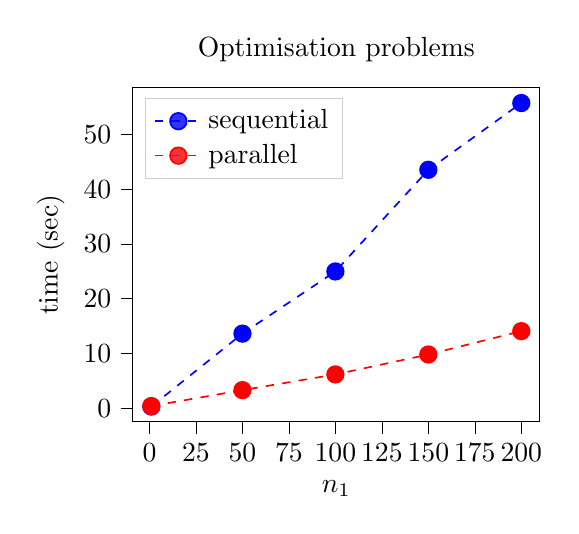
\begin{tikzpicture}

\begin{axis}[
legend cell align={left},
legend style={
  fill opacity=0.8,
  draw opacity=1,
  text opacity=1,
  at={(0.03,0.97)},
  anchor=north west,
  draw=white!80!black
},
tick align=outside,
tick pos=left,
title={Optimisation problems},
x grid style={white!69.0196078431373!black},
xlabel={\(\displaystyle n_1\)},
xmin=-8.95, xmax=209.95,
xtick style={color=black},
xtick={-25,0,25,50,75,100,125,150,175,200,225},
xticklabels={
  \(\displaystyle {\ensuremath{-}25}\),
  \(\displaystyle {0}\),
  \(\displaystyle {25}\),
  \(\displaystyle {50}\),
  \(\displaystyle {75}\),
  \(\displaystyle {100}\),
  \(\displaystyle {125}\),
  \(\displaystyle {150}\),
  \(\displaystyle {175}\),
  \(\displaystyle {200}\),
  \(\displaystyle {225}\)
},
y grid style={white!69.0196078431373!black},
ylabel={time (sec)},
ymin=-2.47820221714874, ymax=58.5401840941498,
ytick style={color=black},
ytick={-10,0,10,20,30,40,50,60},
yticklabels={
  \(\displaystyle {\ensuremath{-}10}\),
  \(\displaystyle {0}\),
  \(\displaystyle {10}\),
  \(\displaystyle {20}\),
  \(\displaystyle {30}\),
  \(\displaystyle {40}\),
  \(\displaystyle {50}\),
  \(\displaystyle {60}\)
}
]
\addplot [semithick, blue, dashed, mark=*, mark size=3, mark options={solid}]
table {%
1 0.295360797001194
50 13.6289079279995
100 24.9877134140006
150 43.5660594969995
200 55.7666210799998
};
\addlegendentry{sequential}
\addplot [semithick, red, dashed, mark=*, mark size=3, mark options={solid}]
table {%
1 0.395076787999642
50 3.30418470500081
100 6.169718268
150 9.81355952200101
200 14.0821000380001
};
\addlegendentry{parallel}
\end{axis}

\end{tikzpicture}

    }
    \resizebox{.49\columnwidth}{!}{%
      % This file was created with tikzplotlib v0.9.12.
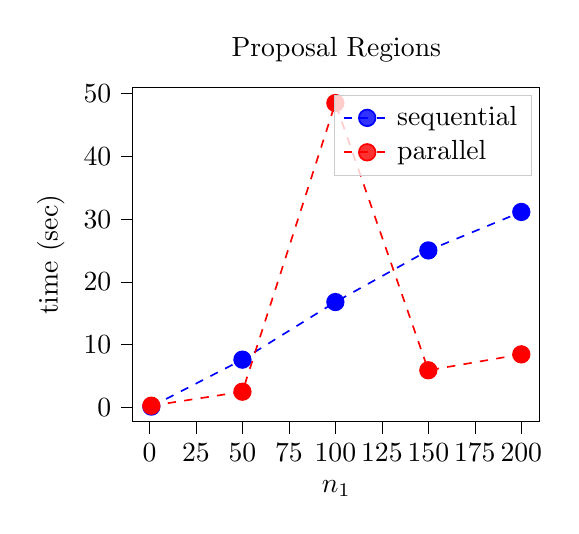
\begin{tikzpicture}

\begin{axis}[
legend cell align={left},
legend style={fill opacity=0.8, draw opacity=1, text opacity=1, draw=white!80!black},
tick align=outside,
tick pos=left,
title={Proposal Regions},
x grid style={white!69.0196078431373!black},
xlabel={\(\displaystyle n_1\)},
xmin=-8.95, xmax=209.95,
xtick style={color=black},
xtick={-25,0,25,50,75,100,125,150,175,200,225},
xticklabels={
  \(\displaystyle {\ensuremath{-}25}\),
  \(\displaystyle {0}\),
  \(\displaystyle {25}\),
  \(\displaystyle {50}\),
  \(\displaystyle {75}\),
  \(\displaystyle {100}\),
  \(\displaystyle {125}\),
  \(\displaystyle {150}\),
  \(\displaystyle {175}\),
  \(\displaystyle {200}\),
  \(\displaystyle {225}\)
},
y grid style={white!69.0196078431373!black},
ylabel={time (sec)},
ymin=-2.26277860274877, ymax=50.8944114557498,
ytick style={color=black},
ytick={-10,0,10,20,30,40,50,60},
yticklabels={
  \(\displaystyle {\ensuremath{-}10}\),
  \(\displaystyle {0}\),
  \(\displaystyle {10}\),
  \(\displaystyle {20}\),
  \(\displaystyle {30}\),
  \(\displaystyle {40}\),
  \(\displaystyle {50}\),
  \(\displaystyle {60}\)
}
]
\addplot [semithick, blue, dashed, mark=*, mark size=3, mark options={solid}]
table {%
1 0.153457309001169
50 7.62618463499894
100 16.8003934079989
150 25.0166328430005
200 31.1416651499985
};
\addlegendentry{sequential}
\addplot [semithick, red, dashed, mark=*, mark size=3, mark options={solid}]
table {%
1 0.295730634999927
50 2.52281142100037
100 48.4781755439999
150 5.93631789100073
200 8.47087084099985
};
\addlegendentry{parallel}
\end{axis}

\end{tikzpicture}

    }
    \end{center}
    \caption[Execution time exploiting parallelisation]{Comparison
      between parallel and sequential execution of the fitting part of
      ROMC. We observe that the parallel version runs between 2.5 an 6
      times faster.}
      \label{fig:exec_parallel}
\end{figure}


%% -- Summary/conclusions/discussion -------------------------------------------
\section{Summary and discussion} \label{sec:summary}
In this paper, we presented the implementation details we followed for
developing the LFI method ROMC at the \pkg{ELFI} package. We paid
thorough attention to two specific use-case scenarios. Firstly, we
illustrate how a user may take advantage of our ready-to-use API for
solving its LFI problem. Secondly, we focus on the scenario where a
researcher wants to intervene and alter parts of the method. Our
implementation is designed to support this as well.

There are still open challenges for the left for future research. Two
directions may enable ROMC to solve high-dimensional problems
efficiently. The first one is enabling ROMC's execution into a cluster
of computers. ROMC can be characterized as an \textit{embarrassingly
  parallel} workload; each optimization problem is an entirely
independent task. Therefore, supporting inference into a cluster of
computers can radically speed up the inference. The second one refers
to implementing the method in a framework that supports automatic
differentiation. Automatic differentiation is necessary for
efficiently solving optimisation problems, especially in
high-dimensional parametric models.


%% -- Optional special unnumbered sections -------------------------------------

\section*{Computational details}

The results in this paper were obtained using \proglang{Python}~3.7.9
with the \pkg{ELFI}~0.8.3 package. The experiments have been executed
in a single machine with an Intel® Core™ i7-8750H Processor an with
Ubuntu 20.04 lts operating system.

\section*{Acknowledgments}

HP was funded by European Research Council grant 742158 (SCARABEE,
Scalable inference algorithms for Bayesian evolutionary epidemiology).

\clearpage
\bibliography{refs}

%% -----------------------------------------------------------------------------

\end{document}
